%\documentclass[10pt,a4paper]{article}
\documentclass[10pt,b5paper]{book}
\usepackage[latin2]{inputenc}
\usepackage[polish]{babel}
\selectlanguage{polish}
\usepackage[OT4]{fontenc}
\usepackage{polski}
\usepackage{ucs}
\usepackage{amsthm}
\usepackage{amsmath}
\usepackage{amsfonts}
\usepackage{array}
\usepackage{tabularx}
\usepackage{makeidx}
%\usepackage{pict2e}

\newcommand{\codomain}{\mathrel{%
  \setlength{\unitlength}{2pt}
  \begin{picture}(6,4)(-1,0)
     \qbezier(3,3.75)(0,2)(3,0.25)
     \qbezier(3,3.75)(4,4)(6,4)
     \qbezier(3,0.25)(4,0)(6,0)
     \qbezier(3,3.75)(0,2)(3,0.25)
     \qbezier(3,3.75)(4,4)(6,4)
     \qbezier(3,0.25)(4,0)(6,0)
     \put(6,0){\line(0,1){4}}
  \end{picture}}}

\newcommand{\domain}{\mathrel{%
  \setlength{\unitlength}{2pt}
  \begin{picture}(6,4)(-2,0)
     \qbezier(3,3.75)(6,2)(3,0.25)
     \qbezier(3,3.75)(2,4)(0,4)
     \qbezier(3,0.25)(2,0)(0,0)
     \qbezier(3,3.75)(6,2)(3,0.25)
     \qbezier(3,3.75)(2,4)(0,4)
     \qbezier(3,0.25)(2,0)(0,0)
     \put(0,0){\line(0,1){4}}
  \end{picture}}}

\makeindex

\usepackage[pdftex]{graphicx}
\usepackage[unicode, colorlinks, pdftex, plainpages=false, hyperindex, pdffitwindow=false, pdfusetitle=true]{hyperref}
  \hypersetup{
    unicode=true
  }
\RequirePackage{color}
%\hypersetup{colorlinks=false}
%\definecolor{KolorLink}{cmyk}{0,0.89,0.94,0.28}
%\definecolor{KolorUrl}{cmyk}{1,1,0,0.5}%<--
\definecolor{KolorLink}{cmyk}{0,0.6,1,0.2}
\definecolor{KolorUrl}{cmyk}{1,0,1,0.28}
\hypersetup{linkcolor=KolorLink,citecolor=KolorLink,urlcolor=KolorUrl}

\newtheorem{twierdzenie}{Twierdzenie}[section]
\newtheorem{definicja}{Definicja}[section]

\author{�ukasz Kusek}
\title{Matematyka - notatki z wyk�adu}
%\institute{Wy�sza Szko�a Oficerska Si� Powietrznych w D�blinie}


\begin{document}

\frontmatter

\begingroup
%% Pocz�tek strony tutu�owej:
\sffamily %%<-- str. tytu�owa sans-serif
\thispagestyle{empty}

\vspace*{\stretch{1}}
\noindent

\makebox[0pt][l]{\begin{minipage}{\textwidth}
\flushright{\Huge\bfseries 
 Matematyka }
\noindent\rule[-1ex]{\textwidth}{3.3pt}\\[2.5ex]
\hfill
 \begingroup
    \emph{\Large notatki z wyk�adu}
 \endgroup
\end{minipage}}

\vspace{\stretch{2}}
\noindent\makebox[0pt][l]{\begin{minipage}{\textwidth}

\flushright
{\bfseries �ukasz Kusek}\\[25mm]
Wy�sza Szko�a Oficerska Si� Powietrznych w D�blinie\\[1.5ex]
\bfseries Wersja robocza z dnia \today
\end{minipage}}

\vspace{\stretch{2}}


\pagebreak
\endgroup

%\maketitle
%\pagebreak

\begingroup
\begin{small}
Copyright \copyright{} 2009-2010 �ukasz Kusek.

Wszelkie prawa zastrze�one.

\bigskip

Kontakt:

tel. +48 509 955 365
\end{small}
\endgroup


% Spis tre�ci
\tableofcontents


% Wst�p
\chapter*{Wst�p}

% Poczatek tresci
\mainmatter

\chapter{Relacje}

\begin{definicja}
Przez \textbf{\emph{par� uporz�dkowan�}}\label{def:para_uporzadkowana}\index{para!uporz�dkowana} $(a, b)$ rozumie� b�dziemy zbi�r pewnych podzbior�w zbioru $\{a,b\}$, a~mianowicie:
\[
(a,b) \quad = \quad \{\{a\}, \{a,b\}\}
\]

\smallskip

\cite[Definicja 1.1.1]{furdzik}
\end{definicja}

\bigskip

\begin{definicja}
\textbf{\emph{Iloczynem kartezja�skim}}\label{def:iloczyn_kartezjanski}\index{iloczyn!kartezja�ski} zbior�w $A$ i~$B$ nazywamy \textbf{zbi�r wszystkich par uporz�dkowanych} $(a,b)$, takich, �e

\begin{itemize}
\item $a \in A$,
\item $b \in B$
\end{itemize}

\noindent i~oznaczmy symbolem

\[
A \times B \quad = \quad \left\{ (a,b) \colon a \in A \wedge b \in B \right\}
\]

\smallskip

\cite[Definicja 1.1.3]{furdzik}
\end{definicja}

\bigskip
%%%%%%%%%%%%%%%%%
\section{Relacja}

\begin{definicja}
\textbf{\emph{Relacj�}}\label{def:relacja}\index{relacja} $\mathcal{R}$ okre�lon� w zbiorach $A$ i~$B$ (zachodz�c� mi�dzy elementami zbior�w $A$ i~$B$) nazywamy \textbf{tr�jk� uporz�dkowan�} (Def. \ref{def:para_uporzadkowana}, str. \pageref{def:para_uporzadkowana})

\[
\left( A, gr\mathcal{R}, B \right)
\]

\noindent gdzie

\begin{itemize}
\item $gr\mathcal{R}$ jest \textbf{podzbiorem iloczynu kartezja�skiego} $A \times B$.
\end{itemize}

\smallskip

\cite[Definicja 1.2.1]{furdzik}
\end{definicja}

\bigskip
\begin{definicja}Niech

\begin{itemize}
\item $a \in A$,
\item $b \in B$.
\end{itemize}

M�wimy, �e element $a$ \textbf{\emph{pozsotaje w relacji}} $\mathcal{R}$ z elementem $b$ ($a \mathcal{R} b$), wtedy i~tylko wtedy, gdy

\[
a \mathcal{R} b \quad \Leftrightarrow \quad (a, b) \; \in \; gr \mathcal{R}
\]

\smallskip

\cite[Definicja 1.2.2]{furdzik}
\end{definicja}

\bigskip
\begin{definicja}
\textbf{\emph{Dziedzin� relacji}}\label{def:dziedzina_relacji}\index{relacja!dziedzina}\index{dziedzina!relacji} ($\domain \mathcal{R}$)

\[
\mathcal{R} \; = \; \left(A, \: gr\mathcal{R}, \: B\right)
\]

\noindent nazywamy \textbf{podzbi�r zbioru} $A$, okre�lony nast�puj�co:

\[
\domain\mathcal{R} \; = \; \left\{ a \in A \colon \; \exists_{b \in B} \quad a \mathcal{R} b \right\}
\]

\smallskip

\cite[Definicja 1.2.3]{furdzik} 
\end{definicja}

\bigskip
\begin{definicja}
\textbf{\emph{Przeciwdziedzin� relacji}}\label{def:przeciwdziedzina_relacji}\index{relacja!przeciwdziedzina}\index{przeciwdziedzina!relacji} ($\codomain \mathcal{R}$)

\[
\mathcal{R} \; = \; \left(A, \: gr\mathcal{R}, \: B\right)
\]

\noindent nazywamy \textbf{podzbi�r zbioru} $B$, okre�lony nast�puj�co:

\[
\codomain \mathcal{R} \; = \; \left\{ b \in B \colon \; \exists_{a \in A} \quad a \mathcal{R} b \right\}
\]

\smallskip

\cite[Definicja 1.2.4]{furdzik}
\end{definicja}

\bigskip
\begin{definicja}
Dana jest relacja 
\[
\mathcal{R} \; = \; \left(A, \: gr\mathcal{R}, \: B\right)
\]

\textbf{\emph{Relacj�}} do niej \textbf{\emph{odwrotn�}}\label{def:relacja_odwrotna}\index{relacja!odwrotna} nazywamy relacj� 

\[
\mathcal{R}^{-1} \; = \; \left(B, \: gr\mathcal{R}^{-1}, \: A\right)
\]

\noindent gdzie

\[
gr \mathcal{R}^{-1} \; = \; \left\{(b,a) \: \in \: B \times A \colon \quad (a,b) \: \in \; gr\mathcal{R} \: \subset \: A \times B\right\}
\]

\smallskip

\cite[Definicja 1.2.5]{furdzik}
\end{definicja}

\medskip

\begin{definicja}
\textbf{\emph{Relacj�}}

\[
\mathcal{R} \; = \; \left(A, \: gr\mathcal{R}, \: B\right)
\]

\noindent nazywamy \textbf{\emph{wsz�dzie okre�lon�}}\label{def:relacja_wszedzie_okreslona}\index{relacja!wsz�dzie okre�lona}, je�eli

\[
\domain \mathcal{R} \; = \; A
\]

\noindent czyli

\[
\forall \: a \in A \quad \exists b \: \in B \colon \qquad (a,b) \: \in \: gr\mathcal{R}
\]

\smallskip

\cite[Definicja 1.2.16]{furdzik}
\end{definicja}


\bigskip

\begin{definicja}
\textbf{\emph{Relacj�}} 

\[
\mathcal{R} \; = \; \left(A, \: gr\mathcal{R}, \: B\right)
\]

\noindent nazywamy \textbf{\emph{surjektywn�}}\label{def:relacja_surjektywna}\index{relacja!surjektywna}, je�eli

\[
\codomain \mathcal{R} \; = \; B
\]

\noindent czyli

\[
\forall \: b \in B \quad \exists \: a \in A \colon \qquad (a,b) \: \in \: gr\mathcal{R}
\]

\smallskip

\cite[Definicja 1.2.17]{furdzik}
\end{definicja}

\bigskip

\begin{definicja}
\textbf{\emph{Relacj�}}

\[
\mathcal{R} \; = \; \left(A, \: gr\mathcal{R}, \: B\right)
\]

\noindent nazywamy \textbf{\emph{injektywn�}}\label{def:relacja_injektywna}\index{relacja!injektywna} (r�nowarto�ciow�)\index{relacja!r�nowarto�ciowa}, je�eli

\begin{tabular*}{\textwidth}%
{@{\extracolsep{\stretch{1}}}lc}
& \\
$\forall \: a_1, a_2 \in A \quad \forall \: b \in B \colon$
& \vspace{0.3cm} \\
\multicolumn{2}{c}{
$\left(a_1, b\right) \in gr\mathcal{R} \; 
\wedge \;
\left(a_2, b\right) \in gr\mathcal{R}
\quad
\Rightarrow
\quad
a_1 = a_2$
\vspace{0.3cm}
}
\end{tabular*}

\smallskip

\cite[Definicja 1.2.18]{furdzik}
\end{definicja}

\bigskip
\begin{definicja}
\textbf{\emph{Relacj�}} $\mathcal{R}$ nazywamy \textbf{\emph{bijektywn�}}\label{def:relacja_bijektywna}, je�eli jest

\begin{itemize}
\item \textbf{suriektywna}
\item i~\textbf{injektywna}.
\end{itemize}
\end{definicja}

\bigskip
%%%%%%%%%%%%%%%%%
\section{Funkcja}

\begin{definicja}
Relacj� 

\[
\mathcal{R} \; = \; \left(A, \: gr\mathcal{R}, \: B\right)
\]

\noindent nazywamy \textbf{\emph{funkcj�}}\label{def:funkcja}\index{funkcja}, je�eli

\begin{tabular*}{\textwidth}%
{@{\extracolsep{\stretch{1}}}lc}
& \\
$\forall \: a \in A \quad \forall \: b_1, b_2 \in B \colon$
& \vspace{0.3cm} \\
\multicolumn{2}{c}{
$\left(a,b_1\right) \in gr\mathcal{R} \; \wedge \; \left(a, b_2\right) \in gr\mathcal{R} \quad \Rightarrow \quad b_1 = b_2$
\vspace{0.3cm}
}
\end{tabular*}

\smallskip

\cite[Definicja 1.2.20]{furdzik}
\end{definicja}

\bigskip

\begin{twierdzenie}
Relacja \textbf{odwrotna} (Def. \ref{def:relacja_odwrotna}, str. \pageref{def:relacja_odwrotna}) do relacji \textbf{injektywnej} (Def. \ref{def:relacja_injektywna}, str. \pageref{def:relacja_injektywna}) jest \textbf{funkcj�}.
\end{twierdzenie}

\bigskip
%%%%%%%%%%%%%%%%%%%%%%
\section{Odwzorowanie}

\begin{definicja}
\textbf{Funkcj�}

\[
\mathcal{R} \; = \; \left(A, \: gr\mathcal{R}, \: B\right)
\]

\noindent \textbf{wsz�dzie okre�lon�} (Def. \ref{def:relacja_wszedzie_okreslona}, str. \pageref{def:relacja_wszedzie_okreslona}) nazywamy \textbf{\emph{odwzorowaniem}}\label{def:odwzorowanie}\index{odwzorowanie} i~oznaczmy

\[
\mathcal{R} \colon \: A \rightarrow B
\]

\smallskip

\cite[Definicja 1.2.21]{furdzik} \cite[Rozdzia� V]{onyszkiewicz}
\end{definicja}



\bigskip
%%%%%%%%%%%%%%%%%%%%%%%%%%%%%%%
\section{Funkcje. Odwzorowania}

\label{podstawowe_definicje_dla_funkcji}
Niech b�d� dane

\begin{itemize}
\item zbi�r $X$
\item zbi�r $Y$
\item relacja (Def. \ref{def:relacja}, str. \pageref{def:relacja})
\[
f \; = \; \left(X, \: gr\: f, \: Y\right)
\]
\end{itemize}

\bigskip

W przypadku gdy \textbf{\emph{relacja}} $f$ jest \textbf{\emph{funkcj�}} (Def. \ref{def:funkcja}, str. \pageref{def:funkcja}) lub \textbf{\emph{odwzorowaniem}} (Def. \ref{def:odwzorowanie}, str. \pageref{def:odwzorowanie}), zamiast m�wi�
\begin{center}
$x$ pozostaje w relacji $f$ z $y$
\end{center}
m�wimy:
\begin{itemize}
\item $x$-owi odpowiada $y$,
\item $x$ przechodzi w $y$,
\item $x$ odwzorowuje si� w $y$,
\item $y$ jest warto�ci� $f$ w $x$, co zapisujemy
\[
y = f(x)
\]
lub
\[
x \rightarrow y = f(x)
\]
\end{itemize}

\bigskip

Zapis $f \; = \; \left(X, \: gr\: f, \: Y\right)$, je�li jest

\medskip

\begin{itemize}
\item \textbf{odwzorowaniem} zapisujemy przez
\[
f \colon \; X \ni \: x \: \rightarrow \: y \quad = \quad  f(x) \: \in Y
\]
lub kr�tko
\[
f \colon \; X \: \rightarrow \: Y
\]
\medskip
i~czytamy \emph{$f$ odworowuje zbi�r $X$ w~zbi�r~$Y$}

\medskip

\item \textbf{funkcj�} to piszemy
\[
f \colon \; X \supset \domain f \ni \: x \: \rightarrow \: y \quad = \quad \: f(x) \: \in Y
\]
lub kr�tko
\[
f \colon \; X \supset \: \domain f \: \rightarrow \: Y
\]
\medskip
i~czytamy \emph{$f$ odwzorowuje swoj� dziedzin� zawart� w~zbiorze~$X$ w~zbi�r~ $Y$}
\end{itemize}

\bigskip

Je�eli $x \rightarrow y = f(x)$ to

\medskip

\begin{itemize}
\item element $y$ nazywamy
\begin{itemize}
\item \textbf{\emph{obrazem}}\index{funkcja!obraz elementu} elementu $x$ poprzez funkcj� (odwzorowanie) $f$
\item \textbf{\emph{warto�ci�}}\index{funkcja!warto��} funkcji (odwzorowania) $f$ w punkcie $x$
\end{itemize}
\item element $x$ nazywamy
\begin{itemize}
\item \textbf{\emph{przeciwobrazem}}\index{funkcja!przeciwobraz elementu} elementu $y$ poprzez funkcj� (odwzorowanie) $f$
\item \textbf{\emph{argumentem}}\index{funkcja!argument} funkcji (odwzorowania) $f$
\end{itemize}
\end{itemize}

\bigskip
%%%%%%%%%%%%%%%%%%%%%%%%%%%%%%%%%%%%%%%%
\subsection{Dziedzina. Przeciwdziedzina}

Zgodnie z definicj� \textbf{\emph{dziedziny relacji}} (Def. \ref{def:dziedzina_relacji}, str. \pageref{def:dziedzina_relacji}) otrzymujemy \label{def:dziedzina_funkcji}\index{dziedzina!funkcji}\index{funkcja!dziedzina}

\[
\domain f \; = \; \left\{x \in X \colon \quad \exists_{y \in Y} \quad y \: = \: f(x)\right\}
\]

\medskip

\noindent jak r�wnie� zgodnie z~definicj� \textbf{\emph{przeciwdziedziny relacji}} (Def. \ref{def:przeciwdziedzina_relacji}, str. \pageref{def:przeciwdziedzina_relacji}) otrzymujemy \label{def:przeciwdziedzina_funkcji}\index{przeciwdziedzina!funkcji}\index{funkcja!przeciwdziedzina}

\[
\codomain f \; = \; \left\{y \in Y \colon \quad \exists_{x \in X} \quad y \: = \: f(x)\right\}
\]

W~przypadku
\begin{itemize}
\item \textbf{\emph{odwzorowania}}

\[
\domain f \: = \: X
\]

\noindent w�wczas zbi�r $X$ nazywamy \textbf{\emph{zbiorem argument�w}}\index{odwzorowanie!zbi�r argument�w}\index{zbi�r!argument�w}

\item \textbf{\emph{funkcji}} na og� (gdy nie jest odwzorowaniem)

\[
\domain f \: \neq \: X, \qquad \domain f \: \subset \: X
\]

\noindent w�wczas zbi�r $X$ nazywamy \textbf{\emph{naddziedzin� funkcji}}\index{funkcja!naddziedzina}.
\end{itemize}

\medskip
Zbi�r $Y$ nazywamy \textbf{\emph{zapasem}} funkcji (odwzorowania)\index{funkcja!zapas}\index{odwzorowanie!zapas}.

\medskip

\cite[Definicja 1.3.1]{furdzik}

\bigskip
%%%%%%%%%%%%%%%%%%%
\subsection{Wykres}

\begin{definicja}
\textbf{\emph{Wykresem}}\label{def:wykres_funkcji} funkcji (odwzorowania) $f$ jest zbi�r

\[
gr \: f \; = \; \left\{(x,y) \; \in \; X \times Y \colon \quad x \: \rightarrow \: y \; = \; f(x)\right\}
\]

\smallskip

\cite[Definicja 1.3.2]{furdzik}
\end{definicja}

\bigskip
%%%%%%%%%%%%%%%%%%%%%%%%%%%%%%%%%%%%%%%%%%
\subsection{Surjekcja. Injekcja. Bijekcja}

\begin{definicja}
\textbf{Funkcj�} (\textbf{odwzorowanie}) nazywamy \textbf{\emph{surjekcj�}}\label{def:surjekcja}

\begin{center}
zbioru $\domain f \subset X$ na $Y$,
\end{center}

\noindent je�eli

\begin{center}
$f$ jest relacj� surjektywn� (Def. \ref{def:relacja_surjektywna}, str. \pageref{def:relacja_surjektywna}).
\end{center}

\smallskip

\cite[Definicja 1.3.2]{furdzik}
\end{definicja}

\medskip

\begin{definicja}
\textbf{Funkcj�} (\textbf{odwzorowanie}) nazywamy \textbf{\emph{injekcj�}}\label{def:injekcja}

\begin{center}
zbioru $\domain f \subset X$ w $Y$,
\end{center}

\noindent je�eli

\begin{center}
$f$ jest relacj� injektywn� (Def. \ref{def:relacja_injektywna}, str. \pageref{def:relacja_injektywna}).
\end{center}

\smallskip

\cite[Definicja 1.3.2]{furdzik}
\end{definicja}

\medskip

\begin{definicja}
\textbf{Odwzorowanie} jest \textbf{\emph{bijekcj�}}\label{def:bijekcja}

\begin{center}
zbioru $X$ na $Y$,
\end{center}

\noindent je�eli jest \textbf{r�wnocze�nie}
\begin{itemize}
\item surjekcj�
\item i injekcj�.
\end{itemize}

\smallskip

\cite[Definicja 1.3.2]{furdzik}
\end{definicja}


\bigskip
%%%%%%%%%%%%%%%%%%%%%%%%%%%%%%%%%%%%%%%%%%%%%%
\subsection{Obraz zbioru. Przeciwobraz zbioru}

\begin{definicja}
\textbf{\emph{Obrazem zbioru}}\index{obraz!zbioru}\index{zbi�r!obraz} $A$ poprzez funkcj� (odwzorowanie) 

\[
f \colon \; X \supset \; \domain f \: \rightarrow \: Y
\]

\noindent nazywamy zbi�r

\[
f[A] \; = \; \left\{y \in Y \colon \quad \exists_{x \in A} \quad x \: \rightarrow \: y \; = \; f(x)\right\}
\]

\smallskip

\cite[Definicja 1.3.3]{furdzik}
\end{definicja}

\bigskip

\begin{definicja}
\textbf{\emph{Przeciwobrazem zbioru}}\index{przeciwobraz!zbioru}\index{zbi�r!przeciwobraz} $B$ poprzez funkcj� (odwzorowanie)

\[
f \colon \; X \supset \; \domain f \: \rightarrow \: Y
\]

\noindent nazywamy zbi�r 

\[
f^{-1}[B] \; = \; \left\{x \in X \colon \quad \exists_{y \in B} \quad x \: \rightarrow \: y \; = \; f(x)\right\}
\]

\smallskip

\cite[Definicja 1.3.3]{furdzik}
\end{definicja}
\chapter{Struktury algebraiczne}

\medskip

Literatura do tego dzia�u: \cite{rut} - 1.1.1, 1.1.2, 1.2.1 \newline
Zadania do tego dzia�u: \cite{rut} - 1.1.1, 1.1.2, 1.2.1

\medskip

\begin{definicja}
\textbf{\emph{Dzia�aniem wewn�trznym}}\label{def:dzialanie_wewnetrzne}\index{dzia�anie}\index{dzia�anie!wewn�trzne} (lub kr�tko \textbf{\emph{dzia�aniem}}\label{def:dzialanie}) w~zbiorze $A$ nazywamy dowolne odwzorowanie (Def. \ref{def:odwzorowanie}, str. \pageref{def:odwzorowanie}) produktu kartezja�skiego (Def. \ref{def:iloczyn_kartezjanski}, str. \pageref{def:iloczyn_kartezjanski})

\begin{center}
$A \times A$ w~zbi�r~$A$.
\end{center}

\smallskip

\cite[Definicja 3, rozdzia� 1.1.1]{rut}
\end{definicja}

\bigskip

\begin{definicja}
M�wimy, �e dzia�anie $\circ$ w zbiorze $A$ jest \textbf{\emph{przemienne}}\label{def:dzialanie_przemienne}\index{dzia�anie!przemienne}, je�li 

\[
\forall \: a,b \in A \colon \qquad a\circ b \; = \; b \circ a
\]

\smallskip

\cite[Definicja 5, rozdzia� 1.1.2]{rut}
\end{definicja}

\bigskip

\begin{definicja}
M�wimy, �e dzia�anie $\circ$ w zbiorze $A$ jest \textbf{\emph{��czne}}\label{def:dzialanie_laczne}\index{dzia�anie!��czne}, je�li 

\[
\forall a, b, c \in A \colon \qquad (a \circ b) \circ c \; = \; a \circ (b \circ c)
\]

\smallskip

\cite[Definicja 6, rozdzia� 1.1.2]{rut}
\end{definicja}

\bigskip

\begin{definicja}
M�wimy, �e element $e \in A$ jest \textbf{\emph{elementem neutralnym}}\label{def:element_neutralny}\index{element!neutralny}\index{dzia�anie!element neutralny} dzia�ania $\circ$ okre�lonego w $A$, je�li

\[
\forall a \in A \colon \qquad a \circ e \; = \; e \circ a \; = \; a
\]

\smallskip

Element neutralny w~notacji

\begin{itemize}
\item multiplikatywnej nazywa si� elementem jednostkowym\index{element!jednostkowy} lub \textbf{\emph{jedynk�}}\label{def:jedynka_dzialania}\index{dzia�anie!jedynka}\index{jedynka!dzia�ania} i~oznacza si� go cz�sto symbolem $\mathbf{1}$.

\item addytywnej nazywamy \textbf{\emph{zerem}}\label{def:zero_dzialania}\index{dzia�anie!zero}\index{zero!dzia�ania} i~oznaczamy go symbolem $\mathbf{0}$.
\end{itemize}

\smallskip

\cite[Definicja 7, rozdzia� 1.1.2]{rut}
\end{definicja}

\bigskip

\begin{definicja}
Niech 

\begin{itemize}
\item dzia�anie $\circ$ w zbiorze $A$ \textbf{ma element neutralny} $e$

\item $a \in A$.
\end{itemize}

\medskip

Ka�dy element $b \in A$ spe�niaj�cy r�wno�� 

\[
a \circ b \; = \; b \circ a \; = \; e
\]

\noindent nazywamy \textbf{\emph{elementem odwrotnym do $a$}}\label{def:element_odwrotny}\index{element!odwrotny}.

\bigskip

Je�li istnieje \textbf{dok�adnie jeden} element odwrotny do $a$, to oznaczamy go symbolem $a^{-1}$.

\medskip

W~notacji addytywnej element odwrotny do $a$ nazywamy \textbf{elementem przeciwnym}\label{def:element_przeciwny}\index{element!odwrotny} do $a$ i~zamiast $a^{-1}$ piszemy~$-a$.

\smallskip

\cite[Definicja 8, rozdzia� 1.1.2]{rut}
\end{definicja} 

\bigskip

\begin{definicja}
Niech w zbiorze $A$ okre�lone b�d� dzia�ania $\odot$ oraz $\oplus$.

\medskip

M�wimy, �e dzia�anie $\odot$ jest \textbf{\emph{rozdzielne}}\label{def:dzialanie_rozdzielne}\index{dzia�anie!rozdzielne} wzgl�dem dzia�ania $\oplus$, je�li

\[
\forall \: a, b, c \in A \colon \qquad a \odot (b \oplus c) \; = \; (a \odot b) \oplus (a \odot c)
\]

\noindent oraz

\[
\forall \: a, b, c \in A \colon \qquad (a \oplus b) \odot c \; = \; (a \odot c) \oplus (b \odot c)
\]

\smallskip

\cite[Definicja 9, rozdzia� 1.1.2]{rut}

\end{definicja}

\bigskip

\begin{definicja}
Niech $A$ i $F$ b�d� dowolnymi zbiorami niepustymi.

\medskip

\textbf{\emph{Dzia�aniem zewn�trznym}}\label{def:dzialanie_zewnetrzne}\index{dzia�anie!zewn�trzne} w~zbiorze $A$ nazywamy dowolne odwzorowanie (Def. \ref{def:odwzorowanie}, str. \pageref{def:odwzorowanie}) produktu kartezja�skiego (Def. \ref{def:iloczyn_kartezjanski}, str. \pageref{def:iloczyn_kartezjanski})

\begin{center}
$F \times A$ w~zbi�r $A$.
\end{center}

\medskip

Zbi�r $F$ nazywamy \emph{zbiorem operator�w}\index{zbi�r!operator�w}.

\smallskip

\cite[Definicja 10, rozdzia� 1.1.3]{rut}.
\end{definicja}

\bigskip

\begin{definicja}
\textbf{\emph{Struktur� algebraiczn�}}\label{def:struktura_algebraiczna}\index{struktura algebraiczna} okre�lon� na zbiorze $A$ nazywamy zesp�

\[
(A; \quad F_1, \ldots, F_m; \quad \circ_1, \ldots, \circ_n; \quad \bullet_1, \ldots, \bullet_m),
\]

\noindent gdzie

\begin{tabular}{m{3cm}m{8cm}m{0,1cm}}
 
$F1, \ldots, F_m \qquad$ &
s� zbiorami, &
 \\[10pt]
 
$\circ_1, \ldots, \circ_n \qquad$ &
s� dzia�aniami wewn�trznymi (Def. \ref{def:dzialanie_wewnetrzne}, str. \pageref{def:dzialanie_wewnetrzne}) w~zbiorze $A$ &
 \\[20pt]
 
$\bullet_1, \ldots, \bullet_m \qquad$ &
s� takimi dzia�aniami zewn�trznymi (Def. \ref{def:dzialanie_zewnetrzne}, str. \pageref{def:dzialanie_zewnetrzne}) w~$A$, �e &
 \\[20pt]
 
&
$\bullet_1 \colon \qquad F_1 \times A \to A, \quad \ldots, \quad F_m \times A \to A$. &
 \\[10pt]
 
\end{tabular}

\smallskip

\cite[Definicja 11, rozdzia� 1.2.1]{rut}
\end{definicja}

\bigskip
%%%%%%%%%%%%%%%%%%%%%
\section{Grupa}

\medskip

\begin{definicja}
\textbf{\emph{Grup�}}\index{grupa} nazywamy par� (Def. \ref{def:para_uporzadkowana}, str. \pageref{def:para_uporzadkowana})

\[
(G, \: \cdot), 
\]

\noindent sk�adaj�c� si�

\begin{itemize}
\item ze zbioru $G$
\item oraz z takiego dzia�ania $\cdot$ (Def. \ref{def:dzialanie}, str. \pageref{def:dzialanie}) okre�lonego w~zbiorze $G$ 

\[
\forall \: a, b \in G \colon \qquad G \times G \in \: (a, b) \: \to \: a + b \: \in G
\]

\noindent kt�re spe�nia warunki:
\begin{enumerate}
\item Dzia�anie $\cdot$ jest \textbf{\emph{��czne}} (Def. \ref{def:dzialanie_laczne}, str. \pageref{def:dzialanie_laczne})
\item Dzia�anie $\cdot$ ma \textbf{\emph{element neutralny}} (Def. \ref{def:element_neutralny}, str. \pageref{def:element_neutralny})
\item Dla ka�dego elementu zbioru $G$ istnieje \textbf{\emph{element odwrotny}} (Def. \ref{def:element_odwrotny}, str. \pageref{def:element_odwrotny})
\end{enumerate}
\end{itemize}

\smallskip

\cite[Definicja 19, rozdzia� 2.1.1]{rut}

\end{definicja}

\bigskip

\begin{definicja}
Grup� $(G, \cdot)$ nazywamy \textbf{\emph{grup� abelow�}}\label{def:grupa_abelowa}\index{grupa!abelowa} (\textbf{\emph{przemienn�}}), je�li dzia�anie $\cdot$ jest \textbf{\emph{przemienne}} (Def. \ref{def:dzialanie_przemienne}, str. \pageref{def:dzialanie_przemienne}). 
\end{definicja}

\bigskip

\begin{definicja}
\textbf{\emph{Elementem neutralnym grupy}}\index{element!neutralny!grupy}\index{grupa!element neutralny} $G$  nazywamy \textbf{\emph{element neutralny dzia�ania}} (Def. \ref{def:element_neutralny}, str. \pageref{def:element_neutralny}), wzgl�dem kt�rego $G$ jest grup�.

\medskip

Element neutralny grupy nazywamy w notacji

\begin{itemize}
\item multiplikatywnej - jedynk� grupy $G$\index{grupa!jedynka}\index{jedynka!dzia�ania},
\item addytywnej - zerem grupy $G$\index{grupa!zero}\index{zero!grupy}.
\end{itemize}

\smallskip

\cite[Definicja 21, rozdzia� 2.1.1]{rut}
\end{definicja}

\bigskip
%%%%%%%%%%%%%%%%%%%%%%%%%
\section{Pier�cie�}

\medskip

\begin{definicja}
Tr�jk� uporz�dkowan� (Def. \ref{def:para_uporzadkowana}, str. \pageref{def:para_uporzadkowana})

\[
(A, \: +, \: \cdot)
\]

\noindent sk�adaj�cy si� z

\begin{itemize}
\item niepustego zbioru $A$,
\item dzia�ania $+$ okre�lonego w~$A$ (Def. \ref{def:dzialanie}, str. \pageref{def:dzialanie})
\item oraz dzia�ania $\cdot$ okre�lonego w~$A$ (Def. \ref{def:dzialanie}, str. \pageref{def:dzialanie})
\end{itemize}

\noindent nazywamy \textbf{\emph{pier�cieniem}}\label{def:pierscien}\index{pier�cie�}, je�li spe�nione s� warunki:

\begin{enumerate}
\item $(A, +)$ jest \textbf{\emph{grup� abelow�}} (Def. \ref{def:grupa_abelowa}, str. \pageref{def:grupa_abelowa})
\item dzia�anie $\cdot$ jest \textbf{\emph{��czne}} (Def. \ref{def:dzialanie_laczne}, str. \pageref{def:dzialanie_laczne})
\item dzia�anie $\cdot$ jest \textbf{\emph{rozdzielne}} (Def. \ref{def:dzialanie_rozdzielne}, str. \pageref{def:dzialanie_rozdzielne}) wzgl�dem $+$
\end{enumerate}
\cite[Definicja 78, rozdzia� 3.1.1]{rut}
\end{definicja}

\bigskip

\begin{definicja}
Je�li dzia�anie $\cdot$ jest \textbf{\emph{przemienne}} (Def. \ref{def:dzialanie_przemienne}, str. \pageref{def:dzialanie_przemienne}), to pier�cie� nazywamy \textbf{\emph{pier�cieniem przemiennym}}\label{def:pierscien_przemienny}\index{pier�cie�!przemienny}.

\smallskip

\cite[Definicja 79, rozdzia� 3.1.1]{rut}
\end{definicja}

\bigskip

\begin{definicja}
\textbf{\emph{Element neutralny dodowania}} (Def. \ref{def:zero_dzialania}, str. \pageref{def:zero_dzialania}) w~pier�cieniu $A$ nazywamy \textbf{\emph{zerem pier�cienia}}\label{def:zero_pierscienia}\index{pier�cie�!zero}\index{zero!pier�cienia} $A$.

\smallskip

\cite[Definicja 80, rozdzia� 3.1.1]{rut}
\end{definicja}

\bigskip

\begin{definicja}
Je�li mno�enie $\cdot$ w pier�cieniu~A ma jedynk� (Def. \ref{def:jedynka_dzialania}, str. \pageref{def:jedynka_dzialania}), to jedynk� t� nazywamy \textbf{\emph{jedynk� pier�cienia}}\label{def:jedynka_pierscienia}\index{pier�cie�!jedynka}\index{jedynka!pier�cienia} $A$ i~m�wimy wtedy, �e $A$ jest \textbf{\emph{pier�cieniem z~jedynk�}}\label{def:pierscien_z_jedynka}\index{pier�cie�!z jedynk�}.

\smallskip

\cite[Definicja 81, rozdzia� 3.1.1]{rut}
\end{definicja}

\bigskip

\begin{definicja}
O~pier�cieniu $A$ m�wimy, �e jest \textbf{\emph{pier�cieniem zerowym}}\label{def:pierscien_zerowy}\index{pier�cie�!zerowy}, je�li zbi�r $A$ jest \textbf{jednoelementowy}.

W~przeciwnym przypadku o~pier�cieniu $A$ m�wimy, �e jest \textbf{\emph{pier�cieniem niezerowym}}\label{def:pierscien_niezerowy}\index{pier�cie�!niezerowy}.

\smallskip

\cite[Definicja 82, rozdzia� 3.1.1]{rut}
\end{definicja}

\bigskip
%%%%%%%%%%%%%%%%%%%%%
\section{Cia�o}

\medskip

\begin{definicja}
\textbf{\emph{Cia�em}}\label{def:cialo}\index{cia�o} nazywamy \textbf{\emph{pier�cie� z jedynk�}} (Def. \ref{def:pierscien_z_jedynka}, str. \pageref{def:pierscien_z_jedynka}) spe�niaj�cy warunki:
\begin{enumerate}
\item zbi�r $K$ ma przynajmniej dwa elementy
\item dla ka�dego elementu zbioru $K$ r�nego od zera grupy $(K, +)$ istnieje element \textbf{\emph{odwrotny}} (Def. \ref{def:element_odwrotny}, str. \pageref{def:element_odwrotny}):
\begin{center}
$\forall \: x \in K, \: x \neq \mathbf{0} \quad \exists \: x^{-1} \colon \qquad x \cdot x^{-1} \; = \; x^{-1} \cdot x  \; = \; \mathbf{1}$
\end{center}
\end{enumerate} 

\smallskip

\cite[Definicja 86, rozdzia� 3.1.4]{rut}
\end{definicja}


\chapter{Przestrze� liniowa (wektorowa)}

\medskip

Literatura do tego dzia�u: \cite{rut}~-~2.1.1, 3.1.1, 3.1.4, \cite{przybylo}~-~3, \cite{kostrykin2}~-~1.1, 1.2, \cite{ptak}~-~9.1, 9.2 \newline
Zadania do tego dzia�u: \cite{rut}~-~2.1.1, 3.1.1, 3.1.4, \cite{przybylo}~-~3.1, 3.2, \cite{ptak}~-~9

\bigskip

\begin{definicja}
\textbf{\emph{Przestrzeni� wektorow�}}\label{def:przestrzen_wektorowa} (\textbf{\emph{przestrzeni� liniow�}}\label{def:przestrzen_liniowa}) nad cia�em (Def. \ref{def:cialo}, str. \pageref{def:cialo}) $(F, +, \cdot)$ nazywamy struktur� algebraiczn� (Def. \ref{def:struktura_algebraiczna}, str. \pageref{def:struktura_algebraiczna}) 

\[
(V, F, \oplus, \odot)
\]

\noindent z�o�on� z:

\begin{itemize}
\item zbioru $V$ - zwanego \emph{zbiorem wektor�w},
\item zbioru $F$ - zwanego \emph{zbiorem skalar�w},
\item dzia�ania $\oplus \colon V \times V \to V$ wewn�trznego (Def. \ref{def:dzialanie_wewnetrzne}, str. \pageref{def:dzialanie_wewnetrzne}) w~zbiorze $V$
\item i~dzia�ania zewn�trznego (Def. \ref{def:dzialanie_zewnetrzne}, str. \pageref{def:dzialanie_zewnetrzne}) $\odot \colon F \times V \to V$,
\end{itemize}

\bigskip

\noindent kt�ra spe�nia nast�puj�ce warunki:

\begin{enumerate}
\item $(V, \oplus)$ jest grup� abelow�
\item $\forall \alpha \in F \quad \forall x,y \in V \colon \qquad \alpha \odot (x \oplus y) = (\alpha \odot x) \oplus (\alpha \odot y)$
\item $\forall \alpha, \beta \in F \quad \forall x \in V \colon \qquad (\alpha + \beta) \odot x = (\alpha \odot x) \oplus (\beta \odot x)$
\item $\forall \alpha, \beta \in F \quad \forall x \in V \colon \qquad \alpha \odot (\beta \odot x) = (\alpha \cdot \beta) \odot x$
\item $\forall x \in V \colon \qquad \qquad \qquad \quad \mathbf{1} \odot x = x$
\end{enumerate}

\smallskip

\cite[Rozdzia� 3]{przybylo}
\end{definicja}

\bigskip
%%%%%%%%%%%%%%%%%%%%%%%%%%%%%%%%%%%%%%%%%%%
\subsection{Kombinacja liniowa wektor�w}

\medskip

Niech $T = {1, \ldots, n}$ oznacza zbi�r wska�nik�w.

\begin{definicja}
Element $x \in V$ przestrzeni $(V, F, \oplus, \odot)$ nazywamy \textbf{\emph{kombinacj� liniow� wektor�w}}\label{def:kombinacja_liniowa_wektorow} $(x_t)_{t \in T}$, je�li istnieje uk�ad skalar�w $(\alpha_t)_{t \in T}$ z~cia�a $F$, taki, �e

\[
x = \sum_{t \in T} \alpha_t x_t
\]

\medskip

Skalary $\alpha_t$ nazywamy \textbf{\emph{wsp�czynnikami}} tej kombinacji liniowej.

\smallskip

\cite[Rozdzia� 3]{przybylo}
\end{definicja}

\bigskip

\begin{definicja}
Uk�ad $(x_t)_{t \in T}$ wektor�w przestrzeni $(V, F, \oplus, \odot)$ nazywamy \textbf{\emph{uk�adem wektor�w liniowo niezale�nych}}\label{def:liniowa_niezaleznosc_wektorow}, je�li dla dowolnego uk�adu $(\alpha_t)_{t \in T}$ skalar�w jest spe�niony warunek

\[
\sum_{t \in T} \alpha_t x_t = 0 \qquad \Rightarrow \qquad \forall t \in T \colon \quad \alpha_t = 0
\]

\smallskip

\cite[Rozdzia� 3]{przybylo}
\end{definicja}

\begin{definicja}
Uk�ad, kt�ry nie jest uk�adem wektor�w liniowo niezale�nych nazywamy \textbf{\emph{uk�adem wektor�w liniowo zale�nych}}\label{def:liniowa_zaleznosc_wektorow}.

\smallskip

\cite[Rozdzia� 3]{przybylo}
\end{definicja}

\bigskip
%%%%%%%%%%%%%%%%%%%%%%%%%%%%%%%%%%%%%%%%%
\subsection{Baza przestrzeni liniowej}

\medskip

\begin{definicja}
\textbf{\emph{Baz� przestrzeni}}\label{def:baza_przestrzeni} $(V, F, \oplus, \odot)$ nazywamy uk�ad wektor�w liniowo niezale�nych $(e_1, \ldots, e_n)$, kt�re generuj� ca�� przestrze�, tzn.

\[
\forall x \in V \quad \exists \alpha_i \in F \colon \qquad x = \sum_i^n \alpha_i e_i
\]

\smallskip

\cite[Rozdzia� 3]{przybylo}
\end{definicja}

\bigskip
%%%%%%%%%%%%%%%%%%%%%%%%%%%%%%%%%%%%%%%%%%%
\subsection{Wymiar przestrzeni liniowej}

\medskip

\begin{definicja}
Moc (liczb� wektor�w) bazy nazywamy \textbf{\emph{wymiarem przestrzeni}}\label{def:wymiar_przestrzeni} $(V,F, \oplus, \odot)$ i~oznaczamy 

\[
\dim V
\]

\smallskip

\cite[Rozdzia� 3]{przybylo}
\end{definicja}



\bigskip
%%%%%%%%%%%%%%%%%%%%%%%%%%%%%%%%%%%%%%%%%%%%
\section{Odwzorowania w przestrzeni linowej}

\medskip

Niech $X$, $Y$, $V_1, \ldots V_n$ oraz $Z$ b�d� przestrzeniami wektorowymi (Def. \ref{def:przestrzen_wektorowa}, str. \pageref{def:przestrzen_wektorowa}) nad cia�em (Def. \ref{def:cialo}, str. \pageref{def:cialo}) $K$.

\medskip

\noindent Niech $W$ oraz $V$ b�d� przestrzeniami wektorowymi (Def. \ref{def:przestrzen_wektorowa}, str. \pageref{def:przestrzen_wektorowa}) nad cia�em liczb zespolonych (Def. \ref{def:liczby_zespolone}, str. \pageref{def:liczby_zespolone}) $\mathbb{C}$.

\bigskip
%%%%%%%%%%%%%%%%%%%%%%%%%%%%%%%%
\subsection{Odwzorowanie linowe}

\begin{definicja}
Odwzorowanie (Def. \ref{def:odwzorowanie}, str. \pageref{def:odwzorowanie}) 

\[
f \colon X \rightarrow Y
\]

\medskip

\noindent nazywamy \textbf{\emph{liniowym}}\label{def:odwzorowanie_liniowe}, je�eli:
\[
\begin{array}{rcl}
\forall x, y \in X & \colon & f(x+y) = f(x) + f(y) \vspace{0.3cm}\\
\forall \alpha \in K \quad \forall x \in X & \colon & f(\alpha \: x) = \alpha \: f(x)
\end{array}
\]

\smallskip

\cite[Definicja 3.4.1]{furdzik}
\end{definicja}

\bigskip
%%%%%%%%%%%%%%%%%%%%%
\subsection{Endomorfizm}

\begin{definicja}
Je�eli

\[
X = Y
\]

\medskip

\noindent to odwzorowanie liniowe (Def. \ref{def:odwzorowanie_liniowe}, str. \pageref{def:odwzorowanie_liniowe}) nazywamy \textbf{\emph{endomorfizmem}}\label{def:endomorfizm}.

\smallskip

\cite[Definicja 3.4.1]{furdzik}
\end{definicja}

\bigskip
%%%%%%%%%%%%%%%%%%%%%%%%%%%%%%%%%%%%
\subsection{Odwzorowanie antylinowe}

\begin{definicja}
Odwzorowanie (Def. \ref{def:odwzorowanie}, str. \pageref{def:odwzorowanie}) 

\[
f \colon W \rightarrow V
\]

\medskip

\noindent nazywamy \textbf{\emph{antyliniowym}}\label{def:odwzorowanie_antyliniowe} (\textbf{\emph{p�liniowym}})\label{def:odwzorowanie_polliniowe}, je�eli:
\[
\begin{array}{rcl}
\forall x, y \in W & \colon & f(x+y) = f(x) + f(y) \vspace{0.3cm}\\
\forall \alpha \in \mathbb{C} \quad \forall x \in W & \colon & f(\alpha \: x) = \overline{\alpha} \: f(x)
\end{array}
\]

\medskip

\noindent Liczba $\overline{\alpha}$ oznacza liczb� sprz�on� (Def. \ref{def:liczba_zespolona_sprzezona}, str. \pageref{def:liczba_zespolona_sprzezona}) z~$\alpha$.
\end{definicja}

\bigskip
%%%%%%%%%%%%%%%%%%%%%%%%%%%%%%%%%%%
\subsection{Odwzorowanie p�toraliniowe}

\begin{definicja}
Odwzorowanie (Def. \ref{def:odwzorowanie}, str. \pageref{def:odwzorowanie}) 

\[
f \colon X \times Y \rightarrow W
\]

\medskip

\noindent nazywamy \textbf{\emph{p�toraliniowym}}\label{def:odwzorowanie_poltoraliniowe}, je�eli jest

\begin{itemize}
\item \textbf{odwzorowaniem liniowym} (Def. \ref{def:odwzorowanie_liniowe}, str. \pageref{def:odwzorowanie_liniowe}) ze wzgl�du na pierwszy argument
\item i~\textbf{odwzorowaniem p�liniowym} (Def. \ref{def:odwzorowanie_polliniowe}, str. \pageref{def:odwzorowanie_polliniowe}) ze wzgl�du na drugi argument
\end{itemize} 
 
czyli
\[
\begin{array}{rcl}
\forall x, x' \in X \quad y \in Y & \colon & f(x+x',y) = f(x,y) + f(x',y) \vspace{0.3cm}\\
\forall \alpha \in \mathbb{C} \quad \forall x \in X \quad \forall y \in Y & \colon & f(\alpha \: x,y) = \alpha \: f(x,y) \vspace{0.3cm}\\
\forall x \in X \quad y, y' \in Y & \colon & f(x,y+y') = f(x,y) + f(x,y') \vspace{0.3cm}\\
\forall \alpha \in \mathbb{C} \quad \forall x \in X \quad \forall y \in Y & \colon & f(x,\alpha \: y) = \overline{\alpha} \: f(x,y)
\end{array}
\]

\medskip

Liczba $\overline{\alpha}$ oznacza liczb� sprz�on� (Def. \ref{def:liczba_zespolona_sprzezona}, str. \pageref{def:liczba_zespolona_sprzezona}) z~$\alpha$.

\smallskip

\cite[Rozdzia� 3.2.1]{kostrykin2}
\end{definicja}

\bigskip
%%%%%%%%%%%%%%%%%%%%%%%%%%%%%%%%%%%%
\subsection{Odwzorowanie dwuliniowe}

\begin{definicja}
Odwzorowanie (Def. \ref{def:odwzorowanie}, str. \pageref{def:odwzorowanie}) 

\[
f \colon X \times Y \rightarrow Z
\]

\medskip

\noindent nazywamy \textbf{\emph{dwuliniowym}}\label{def:odwzorowanie_dwuliniowe}, je�eli jest \textbf{odwzorowaniem liniowym} (Def. \ref{def:odwzorowanie_liniowe}, str. \pageref{def:odwzorowanie_liniowe}) ze wzgl�du na \textbf{ka�d� zmienn�}, czyli
\[
\begin{array}{rcl}
\forall x, x' \in X \quad y \in Y & \colon & f(x+x',y) = f(x,y) + f(x',y) \vspace{0.3cm}\\
\forall \alpha \in K \quad \forall x \in X \quad \forall y \in Y & \colon & f(\alpha \: x,y) = \alpha \: f(x,y) \vspace{0.3cm}\\
\forall x \in X \quad y, y' \in Y & \colon & f(x,y+y') = f(x,y) + f(x,y') \vspace{0.3cm}\\
\forall \alpha \in K \quad \forall x \in X \quad \forall y \in Y & \colon & f(x,\alpha \: y) = \alpha \: f(x,y)
\end{array}
\]

\smallskip

\cite[Definicja 3.9.1]{furdzik} \cite[Rozdzia� 0.2]{trajdos}
\end{definicja}

\bigskip
%%%%%%%%%%%%%%%%%%%%%%%%%%%%%%%%%%%%
\subsection{Odwzorowanie wieloliniowe}

\begin{definicja}
Odwzorowanie (Def. \ref{def:odwzorowanie}, str. \pageref{def:odwzorowanie}) 

\[
f \colon V_1 \times V_2 \times \ldots V_n \rightarrow Z
\]

\medskip

\noindent nazywamy \textbf{\emph{wieloliniowym}}\label{def:odwzorowanie_wieloliniowe} (\textbf{\emph{$n$-liniowym}})\label{def:odwzorowanie_n-liniowe}, je�eli jest \textbf{odwzorowaniem liniowym} (Def. \ref{def:odwzorowanie_liniowe}, str. \pageref{def:odwzorowanie_liniowe}) ze wzgl�du na \textbf{ka�d� zmienn�}.

\smallskip

\cite[Paragraf 1.4.1]{kostrykin2}
\end{definicja}

\bigskip
%%%%%%%%%%%%%%%%%%%%%%%%%%%%%%%%%%%%%%%%%%%%
\section{Formy w przestrzeni linowej}

%%%%%%%%%%%%%%%%%%%%%%%%%%%%%%%%%%%%%%%%%%%%
\subsection{Forma p�toraliniowa}

\begin{definicja}
\textbf{\emph{Form� p�toraliniow�}}\label{def:forma_poltoraliniowa} na iloczynie kartezja�skim (Def. \ref{def:iloczyn_kartezjanski}, str. \pageref{def:iloczyn_kartezjanski}) $X \times Y$ nazywamy \textbf{odwzorowanie p�toraliniowe} (Def. \ref{def:odwzorowanie_poltoraliniowe}, str. \pageref{def:odwzorowanie_poltoraliniowe})

\[
f \colon \; X \times Y \to \mathbb{C}
\]

\smallskip

\cite[Rozdzia� 3.2.1]{kostrykin2}
\end{definicja}

\bigskip
%%%%%%%%%%%%%%%%%%%%%%%%%%%%%%%%%%%%%%%%%%%%
\subsection{Forma dwuliniowa}

\begin{definicja}
\textbf{\emph{Form� dwuliniow�}}\label{def:forma_dwuliniowa} na iloczynie kartezja�skim (Def. \ref{def:iloczyn_kartezjanski}, str. \pageref{def:iloczyn_kartezjanski}) $X \times Y$ nazywamy \textbf{odwzorowanie dwuliniowe} (Def. \ref{def:odwzorowanie_dwuliniowe}, str. \pageref{def:odwzorowanie_dwuliniowe})

\[
f \colon \; X \times Y \to K
\]

\smallskip

\cite[Rozdzia� 0.2]{trajdos}

\bigskip
%%%%%%%%%%%%%%%%%%%%%%%%%%%%%%%%%%%%%%%%%%%%%%%%%%%%
\subsubsection{Posta� analityczna forma dwuliniowej}

Je�eli $dimX = m$ i~$dimY = n$ (Def. \ref{def:wymiar_przestrzeni}, str. \pageref{def:wymiar_przestrzeni}), to form� mo�emy zapisa� w~postaci analitycznej

\[
\begin{array}{ccl}
f(x,y) = a_{ij} \: x^i \: y^j & \qquad & a_{ij} \in K, \; x \in X, \; y \in Y, \vspace{0.3cm}\\
& & i \in \{1, \ldots, m\}, \; j \in \{1, \ldots, n\}
\end{array}
\]

\smallskip

\cite[Rozdzia� 0.2]{trajdos}

\bigskip
%%%%%%%%%%%%%%%%%%%%%%%%%%%%%%%%%%%%%%%%%%%%%%%%%%%
\subsubsection{Posta� macierzowa forma dwuliniowej}

Je�eli $dimX = m$ i $dimY = n$ (Def. \ref{def:wymiar_przestrzeni}, str. \pageref{def:wymiar_przestrzeni}), to form� mo�emy zapisa� w~postaci macierzowej (Def. \ref{def:macierz}, str. \pageref{def:macierz})

\medskip

\[
f(x,y) = \left[x^1, \dots, x^m\right]
\left[
\begin{array}{ccc}
a_{11} & \ldots & a_{1n} \\
\vdots & \ddots & \vdots \\
a_{m1} & \ldots & a_{mn}
\end{array}
\right]
\left[
\begin{array}{c}
y^1  \\
\vdots \\
y^n
\end{array}
\right]
\]

\medskip

\noindent lub przy oznaczeniach kolumnowych

\begin{itemize}
\item $x = \left[x^1, \dots, x^m\right]$,
\item $x^T$ (Def. \ref{def:macierz_transponowana}, str. \pageref{def:macierz_transponowana}),
\item $y = \left[y^1, \dots, y^n\right]$
\item oraz $A = \left[a_{ij} \right]_{m \times n}$
\end{itemize}

\medskip

\[
f(x,y) = x^T \; A \; y
\]

\medskip

\noindent Macierz $A$ nazywamy \textbf{macierz� formy dwulinowej $f$}.

\smallskip

\cite[Rozdzia� 0.2]{trajdos}
\end{definicja}

\bigskip
%%%%%%%%%%%%%%%%%%%%%%%%%%%%%%
\subsection{Forma hermitowska}

\begin{definicja}
Form� p�toraliniow� (Def. \ref{def:forma_poltoraliniowa}, str. \pageref{def:forma_poltoraliniowa})

\[
f \colon \; X \times X \to \mathbb{C}
\]

\medskip

\noindent nazywamy \textbf{\emph{hermitowsk�}}\label{def:forma_hermitowska}, je�li

\[
f(x,y) \; = \; \overline{f(y,x)}
\]

\smallskip

\cite[Paragraf 1.4.4]{kostrykin2}
\end{definicja}

\bigskip
%%%%%%%%%%%%%%%%%%%%%%%%%%%%%%%%%%%%%%%%%
\subsection{Forma dwuliniowa symetryczna}

\begin{definicja}
Form� dwuliniow� (Def. \ref{def:forma_dwuliniowa}, str. \pageref{def:forma_dwuliniowa})

\[
f \colon \; X \times X \to K
\]

\medskip

\noindent nazywamy \textbf{\emph{symetryczn�}}\label{def:forma_dwuliniowa_symetryczna}, je�li

\[
f(x,y) \; = \; f(y,x)
\]

\smallskip

\cite[Paragraf 1.4.4]{kostrykin2}
\end{definicja}

\bigskip
%%%%%%%%%%%%%%%%%%%%%%%%%%%%%%%%%%%%%%%%%
\subsection{Forma dwuliniowa antysymetryczna}

\begin{definicja}
Form� dwuliniow� (Def. \ref{def:forma_dwuliniowa}, str. \pageref{def:forma_dwuliniowa})

\[
f \colon \; X \times X \to K
\]

\medskip

\noindent nazywamy \textbf{\emph{antysymetryczn�}}\label{def:forma_dwuliniowa_antysymetryczna}, je�li

\[
f(x,y) \; = \; -f(y,x)
\]

\smallskip

\cite[Paragraf 1.4.4]{kostrykin2}
\end{definicja}


\bigskip
%%%%%%%%%%%%%%%%%%%%%%%%%%%%%
\subsection{Forma kwadratowa}

\begin{definicja}
Odwzorowanie $g \colon X \to K$ nazywamy \textbf{\emph{form� kwadratow�}}\label{def:forma_kwadratowa} generowan� przez form� dwuliniow� $f$ je�eli:

\[
\forall x \in X \colon \quad g(x) = f(x,x)
\]

\cite[Definicja 4.1.1]{furdzik}
\end{definicja}

\bigskip
%%%%%%%%%%%%%%%%%%%%%%%%%%%%%%%%%%%%%%%
\subsection{Forma dwuliniowa biegunowa}

\begin{definicja}
Jedyn� form� dwuliniow� (Def. \ref{def:forma_dwulinowa}, str. \pageref{def:forma_dwulinowa}), symetryczn� (Def. \ref{def:forma_dwulinowa_symetryczna}, str. \pageref{def:forma_dwulinowa_symetryczna}) generuj�c� form� kwadratow� (Def. \ref{def:forma_kwadratowa}, str. \pageref{def:forma_kwadratowa}) $g$ nazywamy \textbf{\emph{form� biegunow� dla $g$}}\label{def:forma_dwuliniowa_biegunowa}.

\smallskip

\cite[Definicja 4.1.2]{furdzik}
\end{definicja}

\bigskip
%%%%%%%%%%%%%%%%%%%%%%%%%%%%%%%%%%%%%%%%%%%%
\subsection{Forma wieloliniowa}

\begin{definicja}
\textbf{\emph{Form� wieloliniow�}}\label{def:forma_wieloliniowa} (\textbf{\emph{$n$-liniow�}})\label{def:forma_n-liniowa} na iloczynie kartezja�skim (Def. \ref{def:iloczyn_kartezjanski}, str. \pageref{def:iloczyn_kartezjanski}) $V_1 \times V_2 \times \ldots \times V_n$ nazywamy \textbf{odwzorowanie wieloliniowe} (\textbf{$n$-liniowe}) (Def. \ref{def:odwzorowanie_wieloliniowe}, str. \pageref{def:odwzorowanie_wieloliniowe})

\[
f \colon \; V_1 \times V_2 \times \ldots V_n \to K
\]

\smallskip

\cite[Paragraf 1.4.1]{kostrykin2}
\end{definicja}

\bigskip
%%%%%%%%%%%%%%%%%%%%%%%%%%%%%%%%%%%%%%%%%%%
\subsection{Forma wieloliniowa symetryczna}

\begin{definicja}
Form� wieloliniow� ($n$-liniow�) (Def. \ref{def:forma_wieloliniowa}, str. \pageref{def:forma_wieloliniowa})

\[
f \colon \; X^n \to K
\]

\medskip

\noindent nazywamy \textbf{\emph{symetryczn�}}\label{def:forma_wieloliniowa_symetryczna}, je�li

\[
f(x_{{i_1}1},x_{{i_2}2}, \ldots, x_{{i_n}n}) \; = \; f(x_1,x_2, \ldots, x_n)
\]

\smallskip

\cite[Paragraf 1.4.1]{kostrykin2}
\end{definicja}

\bigskip
%%%%%%%%%%%%%%%%%%%%%%%%%%%%%%%%%%%%%%%%%%%
\subsection{Forma wieloliniowa antysymetryczna}

\begin{definicja}
Form� wieloliniow� ($n$-liniow�) (Def. \ref{def:forma_wieloliniowa}, str. \pageref{def:forma_wieloliniowa})

\[
f \colon \; X^n \to K
\]

\medskip

\noindent nazywamy \textbf{\emph{antysymetryczn�}}\label{def:forma_wieloliniowa_antysymetryczna}, je�li

\[
f(x_{{i_1}1},x_{{i_2}2}, \ldots, x_{{i_n}n}) \; = \; \textsl{sgn}(i_1,i_2, \ldots, i_n) \; f(x_1,x_2, \ldots, x_n)
\]

\medskip

\noindent gdzie sumowanie rozci�ga si� na wszystkie permutacje (Def. \ref{def:permutacja}, str. \pageref{def:permutacja}) $(i_1, i_2, \ldots, i_n)$ zbioru $\{1, 2, \ldots , n\}$.

\smallskip

\cite[Paragraf 1.4.1]{kostrykin2}
\end{definicja}

\bigskip
%%%%%%%%%%%%%%%%%%%%%%%%%%%%%%%%%%%%%%%%%%%%%%%%%%%%%
\section{Przestrze� unitarna. Iloczyn skalarny}

%%%%%%%%%%%%%%%%%%%%%%%%%%%%%
\subsection{Iloczyn skalarny}

\medskip

\begin{definicja}
Niech
\begin{itemize}
\item $V$ b�dzie \textbf{przestrzeni� wektorow�} (Def. \ref{def:przestrzen_wektorowa}, str. \pageref{def:przestrzen_wektorowa}) nad \textbf{cia�em liczb zespolonych} (Def. \ref{def:liczby_zespolone}, str. \pageref{def:liczby_zespolone}) $\mathbb{C}$
\item $g \colon V \rightarrow \mathbb{C}$ pewn� \textbf{form� kwadratow�} (Def. \ref{def:forma_kwadratowa}, str. \pageref{def:forma_kwadratowa}) \textbf{okre�lon� dodatnio}
\end{itemize}

\medskip

\noindent \textbf{Form� hermitowsk�} (Def. \ref{def:forma_hermitowska}, str. \pageref{def:forma_hermitowska})~$f$ generuj�c� form� kwadratow�~$g$ nazywamy \textbf{\emph{iloczynem skalarnym}}\label{def:iloczyn_skalarny_przestrzen_unitarna} okre�lonym w~$V$.

\medskip
\noindent Warto�� formy $f(x,y)$ oznaczamy $(x|y)$ lub $x \circ y$.

\smallskip

\cite[Paragraf 3.2.1]{kostrykin2}
\end{definicja}

\bigskip
%%%%%%%%%%%%%%%%%%%%%%%%%%%%%%%%%%%%%%%%%%%%%
\subsubsection{W�asno�ci iloczynu skalarnego}

\label{wl:iloczyn_skalarny_przestrzen_unitarna}

\[
\begin{array}{lrcl}
1. & \forall x, y \in V & \colon & (x|y)= \overline{(y|x)} \vspace{0.3cm}\\
2. & \forall \alpha \in \mathbb{C} \quad \forall x,y \in V & \colon & (\alpha x|y) = \alpha(x|y) \vspace{0.3cm}\\
3. & \forall x_1, x_2, y \in V & \colon & (x_1 + x_2|y) = (x_1|y) + (x_2|y) \vspace{0.3cm}\\
4. & \forall x \in V & \colon & re(x|x) \geq 0 \qquad \textsl{ oraz } \qquad (x|x) = 0 \Leftrightarrow x = 0
\end{array}
\]

\smallskip

\cite[Rozdzia� 6]{przybylo} \cite[Paragraf 3.2.1]{kostrykin2}

\bigskip
%%%%%%%%%%%%%%%%%%%%%%%%%%%%%%%%%%%
\subsection{Przestrze� unitarna}

\begin{definicja}
Przestrze� $V$ nad cia�em $\mathbb{C}$, w kt�rej okre�lono iloczyn skalarny nazywamy \textbf{\emph{przestrzeni� unitarn�}}\label{def:przestrzen_unitarna}.

\smallskip

\cite[Rozdzia� 6]{przybylo} \cite[Paragraf 3.2.1, Definicja 2]{kostrykin2}
\end{definicja}

\bigskip

%%%%%%%%%%%%%%%%%%%%%%%%%%%%%
\subsection{Norma wektora}

\begin{definicja}
\textbf{\emph{D�ugo�ci�}}\label{def:dlugosc_wektora_unitarna} lub \textbf{\emph{norm�}}\label{def:norma_wektora_unitarna} wektora $v \in V$ nazywamy liczb� rzeczywist� nieujemn�

\[
\|v\| \; = \; \sqrt{(v|v)}
\]

\smallskip

\cite[Rozdzia� 3.2.1]{kostrykin2}
\end{definicja}

\bigskip
%%%%%%%%%%%%%%%%%%%%%%%%%%%%%%%%%%%%%%%%%%%%%%%%%%%%%%%%
\section{Przestrze� euklidesowa. Iloczyn skalarny}

%%%%%%%%%%%%%%%%%%%%%%%%%%%%%%%%%%%%%%%%%%%%%
\subsection{Iloczynu skalarny}

\medskip

\begin{definicja}
Niech
\begin{itemize}
\item $V$ b�dzie \textbf{przestrzeni� wektorow�} (Def. \ref{def:przestrzen_wektorowa}, str. \pageref{def:przestrzen_wektorowa}) nad \textbf{cia�em liczb rzeczywistych} $\mathbb{R}$ (TODO cia�o liczb rzeczywistych?)
\item $g \colon V \rightarrow \mathbb{R}$ pewn� \textbf{form� kwadratow�} (Def. \ref{def:forma_kwadratowa}, str. \pageref{def:forma_kwadratowa}) \textbf{okre�lon� dodatnio}
\end{itemize}

\medskip

\noindent \textbf{Form� dwuliniow� $f$ biegunow�} (Def. \ref{def:forma_dwuliniowa_biegunowa}, str. \pageref{def:forma_dwuliniowa_biegunowa}) dla~$g$ nazywamy \textbf{\emph{iloczynem skalarnym}}\label{def:iloczyn_skalarny_przestrzen_euklidesowa} okre�lonym w~$V$.

\medskip
\noindent Warto�� formy $f(x,y)$ oznaczamy $(x|y)$ lub $x \circ y$.

\smallskip

\cite[Definicja 4.1.6]{furdzik} \cite[Paragraf 3.2.1]{kostrykin2}
\end{definicja}

\bigskip
%%%%%%%%%%%%%%%%%%%%%%%%%%%%%%%%%%%%%%%%%%%%%
\subsubsection{W�asno�ci iloczynu skalarnego}

\label{wl:iloczyn_skalarny_przestrzen_euklidesowa}

\[
\begin{array}{lrcl}
1. & \forall x, y \in V & \colon & (x|y)= (y|x) \vspace{0.3cm}\\
2. & \forall \alpha \in \mathbb{R} \quad \forall x,y \in V & \colon & (\alpha x|y) = \alpha(x|y) \vspace{0.3cm}\\
3. & \forall x_1, x_2, y \in V & \colon & (x_1 + x_2|y) = (x_1|y) + (x_2|y) \vspace{0.3cm}\\
4. & \forall x \in V & \colon & (x|x) \geq 0 \qquad \textsl{ oraz } \qquad (x|x) = 0 \Leftrightarrow x = 0
\end{array}
\]

\smallskip

\cite[Rozdzia� 6]{przybylo} \cite[Paragraf 3.2.1]{kostrykin2}

\bigskip
%%%%%%%%%%%%%%%%%%%%%%%%%%%%%%%%%%%%%%
\subsection{Przestrze� euklidesowa}

TODO kt�ra definicja bardziej prawdziwa?

\begin{definicja}
Przestrze� $V$ nad cia�em $\mathbb{R}$, w kt�rej okre�lono iloczyn skalarny, nazywamy \textbf{\emph{przestrzeni� euklidesow�}}\label{def:przestrzen_euklidesowa}.

\smallskip

\cite[Rozdzia� 6]{przybylo}
\end{definicja}

\begin{definicja}
Przestrze� $\mathbb{R}^n$ z

\begin{itemize}
\item iloczynem skalarnym (Def. \ref{def:iloczyn_skalarny_przestrzen_euklidesowa}, str. \pageref{def:iloczyn_skalarny_przestrzen_euklidesowa})

\[
(x|y) \; = \; \sum_{i=1}^n x_i \: y_i
\]

\item i~norm� wektora (Def. \ref{def:norma_wektora_euklidesowa}, str. \pageref{def:norma_wektora_euklidesowa})

\[
\|v\|=\sqrt{(v|v)}
\]

\end{itemize}

\noindent nazywamy \textbf{\emph{przestrzeni� euklidesow�}} i~oznaczamy $\overrightarrow{E_n}$

\smallskip

\cite[Definicja 4.1.7]{furdzik}
\end{definicja}

\bigskip

%%%%%%%%%%%%%%%%%%%%%%%%%%%%%%%%%%%%%%%%%%%%%%%%%%%%%%%%%%%%%%%%%%%%%%%%%%%%
\subsection{Baza ortogonalna, baza ortonormalna przestrzeni euklidesowej}

\begin{definicja}
Baz� (Def. \ref{def:baza_przestrzeni}, str. \pageref{def:baza_przestrzeni}) 

\[
(e_1, \ldots, e_n)
\]

\noindent przestrzeni euklidesowej $V$ nazywamy \textbf{\emph{ortogonaln�}}\label{def:baza_ortogonalna}, je�li 

\[
(e_i|e_j) = 0
\]

\noindent dla dowolnych $i \neq j \quad (i,j = 1, \ldots, n)$.

\smallskip

\cite[Definicja 4, rozdzia� 3.1]{kostrykin2}
\end{definicja}

\bigskip

\begin{definicja}
Baz� \textbf{ortogonaln�} (Def. \ref{def:baza_ortogonalna}, str. \pageref{def:baza_ortogonalna})

\[
(e_1, \ldots, e_n)
\]

\noindent przestrzeni euklidesowej $V$ nazywamy \textbf{\emph{ortonormaln�}}\label{def:baza_ortonormalna}, je�li

\[
(e_i|e_i) = 1
\]

\noindent dla ka�dego $i$.

\smallskip

\cite[Definicja 4, rozdzia� 3.1]{kostrykin2}
\end{definicja}

\bigskip

%%%%%%%%%%%%%%%%%%%%%%%%%%%%%
\subsection{Norma wektora}

\begin{definicja}
\textbf{\emph{D�ugo�ci�}}\label{def:dlugosc_wektora_euklidesowa} lub \textbf{\emph{norm�}}\label{def:norma_wektora_euklidesowa} wektora $v \in V$ nazywamy liczb� rzeczywist� nieujemn�

\[
\|v\| \; = \; \sqrt{(v|v)}
\]

\smallskip

\cite[Definicja 2, rozdzia� 3.1]{kostrykin2}
\end{definicja}

\bigskip
%%%%%%%%%%%%%%%%%%%%%%%%%%%%%%
\section{Przestrze� afiniczna}

TODO sprawdzic czy $\chi$ czy $X$ jest przestrzeni� afiniczna (jesli $X$ to zmienic w geometrii analitycznej)

\begin{definicja}
Uporz�dkowan� tr�jk�

\[
\chi \; = \; (X, V, +)
\]

\medskip

\noindent nazywa� b�dziemy \textbf{\emph{przestrzeni� afiniczn�}}\label{def:przestrzen_afiniczna} je�eli

\begin{itemize}
\item $X$ b�dzie pewnym zbiorem
\item $V$ - przestrzeni� wektorow� (Def. \ref{def:przestrzen_wektorowa}, str. \pageref{def:przestrzen_wektorowa})
\item $+$ - dzia�aniem zewn�trznym (Def. \ref{def:dzialanie_zewnetrzne}, str. \pageref{def:dzialanie_zewnetrzne}) w~$X$

\[
X \: \times \: Y \; \ni \; (x,v) \quad \rightarrow \quad x + v \; \in \; X
\]

spe�niaj�cym warunki:

\begin{tabular}{m{0,2cm}m{3,8cm}m{0,1cm}m{4,6cm}m{0,1cm}}
 
1. &
$\forall x \in X$ &
$:$ &
$x + \mathbf{0} \; = \; x \qquad (\mathbf{0} \in V)$ &
 \\[10pt]
 
2. &
$\forall x,y \in X \quad \exists v \in V $ &
$:$ &
$x + v \; = \; y$ &
 \\[10pt]
 
3. &
$\forall x \in X \quad \forall v_1, v_2 \in V$ &
$:$ &
$x + v_1 = x + v_2 \; \Rightarrow \; v_1 = v_2$ TODO sprawdzic &
 \\[10pt]
 
4. &
$\forall x \in X \quad \forall u,v \in V$ &
$:$ &
$x + (u + v) \; = \; (x + u) + v$ &
 \\[10pt]

\end{tabular}

\end{itemize}

\smallskip

\cite[Definicja 3.5.1]{furdzik}
\end{definicja}

\bigskip
%%%%%%%%%%%%%%%%%%%%%%%%%%%%%%%%%%%%%%%%%%%
\subsection{Przestrze� wektor�w swobodnych}

\begin{definicja}
Przestrze� wektorow� $V$ przestrzeni afinicznej $\chi$ nazywamy \textbf{przestrzeni� wektor�w swobodnych przestrzeni afinicznej}\label{def:przestrzen_wektorow_swobodnych} $X$ i~oznacza� b�dziemy

\[
\vec{X}
\]

\smallskip

TODO sprawdzi� 'przestrzeni afinicznej $X$'

\cite[Definicja 3.5.1]{furdzik}
\end{definicja}

\bigskip
%%%%%%%%%%%%%%%%%%%%%%%%%%%%
\subsection{R�nica punkt�w}

\begin{definicja}
\textbf{\emph{R�nic� punkt�w}}\label{def:roznica_punktow} $x$ i $y$ ($x,y \in X$) lub \textbf{\emph{wektorem ��cz�cym punkty}} $x$ i $y$ nazywamy \textbf{jedyny wektor} spe�niaj�cy aksjomat~2 definicji przestrzeni afinicznej (Def. \ref{def:przestrzen_afiniczna}, str. \pageref{def:przestrzen_afiniczna}).

\medskip

Oznaczmy

\[
y - x \qquad \textsl{lub} \qquad \overrightarrow{xy}
\]

\smallskip

\cite[Definicja 3.5.1]{furdzik}
\end{definicja}

\bigskip
%%%%%%%%%%%%%%%%%%%%%%%%%%%%%%%%
\subsection{Uk�ad wsp�rz�dnych}

\begin{definicja}
\textbf{\emph{Uk�adem wsp�rz�dnych}}\label{def:uklad_wspolrzednych} w~$n$-wymiarowej (Def. \ref{def:wymiar_przestrzeni}, str. \pageref{def:wymiar_przestrzeni}) przestrzeni afinicznej $\chi$ (Def. \ref{def:przestrzen_afiniczna}, str. \pageref{def:przestrzen_afiniczna}) nazywamy par�

\[
(o; \; e_1, \ldots, e_n)
\]

\noindent z�o�on� z

\begin{itemize}
\item punktu $o \in X$
\item i~bazy (Def. \ref{def:baza_przestrzeni}, str. \pageref{def:baza_przestrzeni}) $(e_1, \ldots, e_n)$ w $V$
\end{itemize}

\smallskip

\cite[Paragraf 4.1.3, Definicja 3]{kostrykin2}
\end{definicja}

\bigskip

\begin{definicja}
\textbf{\emph{Wsp�rz�dnymi}} 

\[
x_1, \ldots, x_n
\]

\noindent \textbf{\emph{punktu}}\label{def:wspolrzedne_punktu} $p$ w~uk�adzie $(o; \; e_1, \ldots, e_n)$ nazywamy wsp�rz�dne wektora $\overrightarrow{op}$ w~bazie $(e_1, \ldots, e_n)$

\[
\overrightarrow{op} \; = \; x_1 e_1 + \ldots + x_n e_n
\]

\smallskip

\cite[Paragraf 4.1.3, Definicja 3]{kostrykin2}
\end{definicja}




\chapter{Algebra Boole'a}

\begin{definicja}
\textbf{\emph{Algebra Boole'a}}\index{algebra!Boole'a} to struktura algebraiczna (Def. \ref{def:struktura_algebraiczna}, str. \pageref{def:struktura_algebraiczna})

\[
\mathbb{B} = \left(\mathbf{B}, \cup, \cap, \overline{\phantom{0}}, 0, 1\right),
\]

\noindent w kt�rej

\begin{itemize}
\item $\cup$ i $\cap$ s� dzia�aniami dwuargumentowymi,
\item $\overline{\phantom{0}}$ jest dzia�aniem jednoargumentowym,
\item a $0$ i $1$ s� \emph{wyr�nionymi, r�nymi} elementami zbioru $\mathbf{B}$,
\end{itemize}

\medskip

\noindent spe�niaj�ca nast�puj�ce warunki:

\begin{enumerate}
\item dzia�anie $\cup$ jest \textbf{przemienne} (Def. \ref{def:dzialanie_przemienne}, str. \pageref{def:dzialanie_przemienne})
\item dzia�anie $\cup$ jest \textbf{��czne} (Def. \ref{def:dzialanie_laczne}, str. \pageref{def:dzialanie_laczne})
\item aksjomat Huntingtona\index{aksjomat!Huntingtona}: 

\[
\forall \: x, y \in B \qquad \Rightarrow \qquad \overline{\left( \overline{x} \cup \overline{y} \right)} \cup \overline{\left(\overline{x} \cup y \right)} \; = \; x
\]
\end{enumerate}
\end{definicja}

\medskip

\begin{definicja}
\textbf{\emph{Elementem jednostkowym}}\label{def:element_jednostkowy} nazywamy element $\mathbf{1}$ taki, �e:

\[
\forall \: x \in B \colon \qquad x \cup \overline{x} \; = \; \mathbf{1}
\]
\end{definicja}

\medskip

\begin{definicja}
\textbf{\emph{Elementem zerowym}}\label{def:element_zerowy} nazywamy element $\mathbf{0}$ taki, �e:

\[
\forall \: x \in B \colon \qquad \overline{x \cup \overline{x}} \; = \; \mathbf{0}
\]
\end{definicja}

\medskip

\begin{definicja}
\textbf{\emph{Dzia�anie $\cap$}}:
\[
\forall \; x,y \in B \colon \qquad x \cap y \; = \; \overline{\overline{x} \cup \overline{y}}
\]
\end{definicja}

\bigskip

%%%%%%%%%%%%%%%%%%%%%%%%%%%
\section{Tabela dzia�a�}

$\alpha$, $\beta$ - zdania (formy zdaniowe, kt�rym mo�na przypisa� warto��)

\medskip

\begin{tabular}{|c|c|c|c|c|c|c|}
\hline
$\alpha$ & $\beta$ & $\overline{\alpha}$ & $\alpha \vee \beta$ & $\alpha \wedge \beta$ & $\alpha \Rightarrow \beta$ & $\alpha \Leftrightarrow \beta$ \\
\hline
0 & 0 & 1 & 0 & 0 & 1 & 1 \\
0 & 1 & 1 & 1 & 0 & 1 & 0 \\
1 & 0 & 0 & 1 & 0 & 0 & 0 \\
1 & 1 & 0 & 1 & 1 & 1 & 1 \\
\hline
\end{tabular}

\bigskip
%%%%%%%%%%%%%%%%%%%%%%%%%%%%%%%%%%%%%%%%%%%%
\section{Twierdzenia dla Algebry Boole'a}

\begin{twierdzenie}[o unikalno�ci]
Jest \textbf{tylko jeden} element jednostkowy~$\mathbf{1}$ (Def. \ref{def:element_jednostkowy}, str. \pageref{def:element_jednostkowy}).

Jest \textbf{tylko jeden} element zerowy~$\mathbf{0}$ (Def. \ref{def:element_zerowy}, str. \pageref{def:element_zerowy}).
\end{twierdzenie}

\medskip

\begin{twierdzenie}[o dope�nianiu]
\[
x \cup \overline{x} \; = \; \mathbf{1}
\]
\[
x \cap \overline{x} \; = \; \mathbf{0}
\]
\end{twierdzenie}

\medskip

\begin{twierdzenie}[o podw�jnej negacji]
\[
\overline{\overline{x}} \; = \; x
\]
\end{twierdzenie}

\medskip

\begin{twierdzenie}[prawa De Morgana]
\[
\overline{x \cup y} \; = \; \overline{x} \cap \overline{y}
\]
\[
\overline{x \cap y} \; = \; \overline{x} \cup \overline{y}
\]
\end{twierdzenie}

\medskip

\begin{twierdzenie}
\[
x \cap x \; = \; x
\quad
x \cup x \; = \; x
\quad
x \cup \mathbf{0} \; = \; x
\quad
x \cup \mathbf{1} \; = \; \mathbf{1}
\quad
x \cap \mathbf{1} \; = \; x
\quad
x \cap \mathbf{0} \; = \; \mathbf{0}
\]
\end{twierdzenie}

\medskip

\begin{twierdzenie}[o rozdzielno�ci]
\[
x \cup \left(y \cap z \right) \; = \; \left(x \cup y \right) \cap \left(x \cup z \right)
\]
\[
x \cap \left(y \cup z\right) \; = \; \left(x \cap y\right) \cup \left(x \cap z\right)
\]
\end{twierdzenie}

\bigskip
%%%%%%%%%%%%%%%%%%%%%%%%%%%%%%%%%%%%%%%%%%%%%%%%%%%%%%%%
\section{Funktory w elektrotechnice. Bramki logiczne}

\smallskip
%%%%%%%%%%%%%%%%%%%%%%%%%%
\subsection{Bramka NOT}
\index{bramka!NOT}

\begin{tabular}{m{6cm}m{7cm}m{0.1cm}}
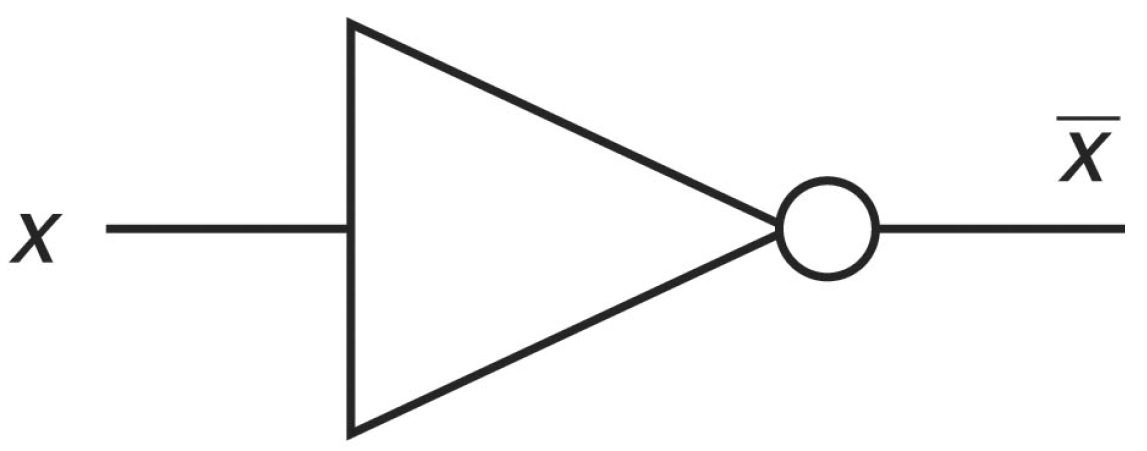
\includegraphics[width=4cm]{img/gates-not.png} &
\begin{tabular}{|m{1cm}|m{1cm}|m{0.1cm}}
\cline{1-2} $x$ & $\overline{x}$ &\\[1em]
\cline{1-2} 0 & 1 &\\[0.3em]
1 & 0 &\\[0.3em]
\cline{1-2}
\end{tabular}
& \\
\end{tabular}


\bigskip
%%%%%%%%%%%%%%%%%%%%%%%%%
\subsection{Bramka OR}
\index{bramka!OR}

\begin{tabular}{m{6cm}m{7cm}m{0.1cm}}
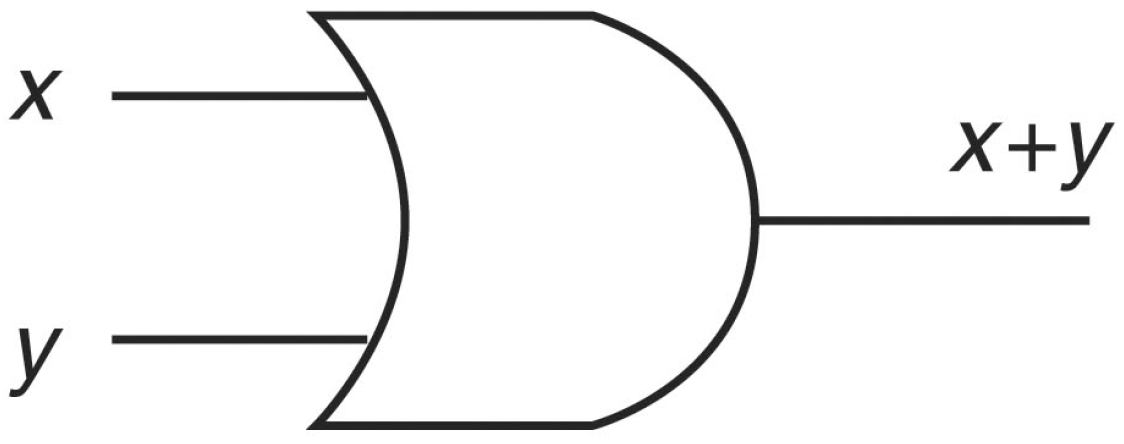
\includegraphics[width=4cm]{img/gates-or.png} &
\begin{tabular}{|m{1cm}|m{1cm}|m{1cm}|m{0.1cm}}
\cline{1-3} $x$ & $y$ & $x \vee y$ &\\[1em]
\cline{1-3} 0 & 0 & 0 &\\[0.3em]
0 & 1 & 1 &\\
1 & 0 & 1 &\\
1 & 1 & 1 &\\[0.3em]
\cline{1-3}
\end{tabular}
& \\
\end{tabular}

\bigskip
%%%%%%%%%%%%%%%%%%%%%%%%%%
\subsection{Bramka NOR}
\index{bramka!NOR}

\begin{tabular}{m{6cm}m{7cm}m{0.1cm}}
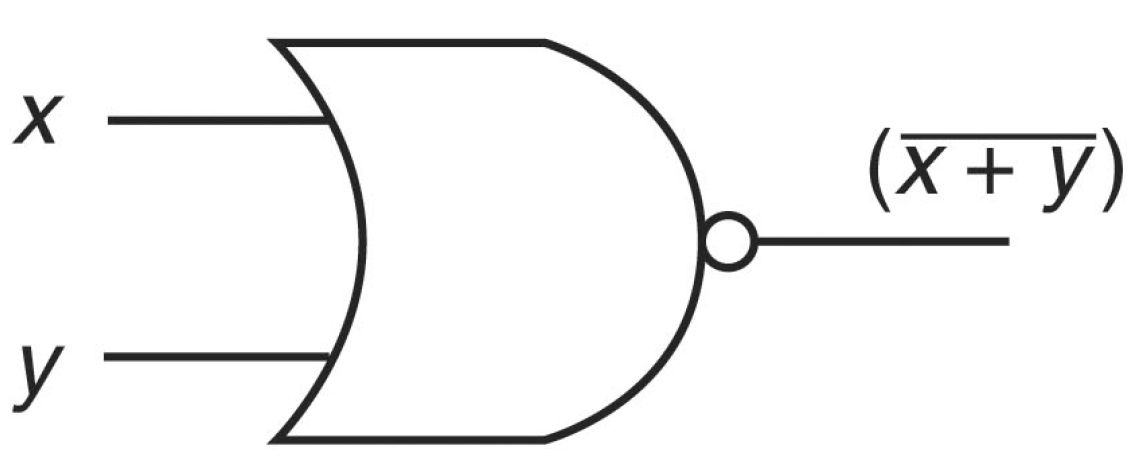
\includegraphics[width=4cm]{img/gates-nor.png} &
\begin{tabular}{|m{1cm}|m{1cm}|m{1cm}|m{0.1cm}}
\cline{1-3} $x$ & $y$ & $\overline{x \vee y}$ &\\[1em]
\cline{1-3} 0 & 0 & 1 &\\[0.3em]
0 & 1 & 0 &\\
1 & 0 & 0 &\\
1 & 1 & 0 &\\[0.3em]
\cline{1-3}
\end{tabular}
& \\
\end{tabular}


\bigskip
%%%%%%%%%%%%%%%%%%%%%%%%%%
\subsection{Bramka AND}
\index{bramka!AND}

\begin{tabular}{m{6cm}m{7cm}m{0.1cm}}
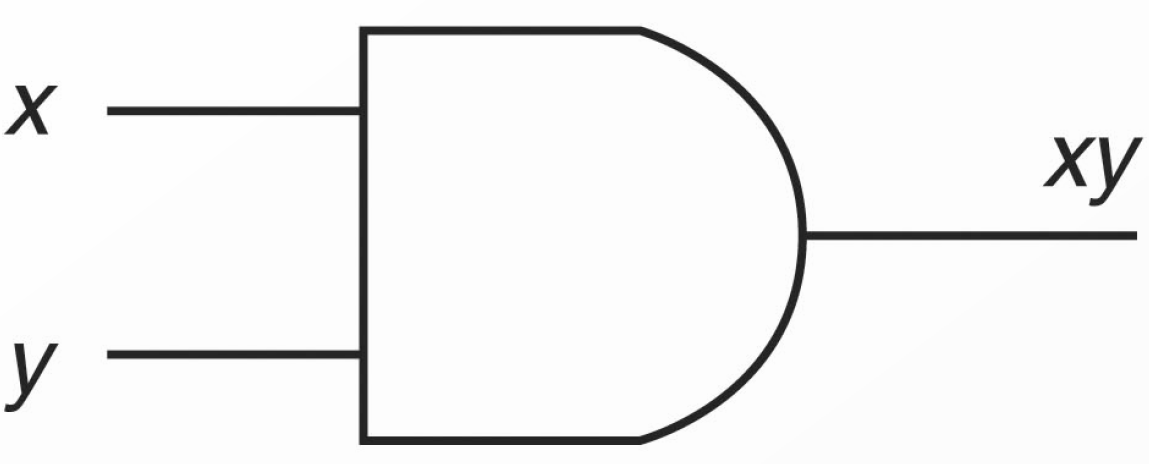
\includegraphics[width=4cm]{img/gates-and.png} &
\begin{tabular}{|m{1cm}|m{1cm}|m{1cm}|m{0.1cm}}
\cline{1-3} $x$ & $y$ & $x \wedge y$ &\\[1em]
\cline{1-3} 0 & 0 & 0 &\\[0.3em]
0 & 1 & 0 &\\
1 & 0 & 0 &\\
1 & 1 & 1 &\\[0.3em]
\cline{1-3}
\end{tabular}
& \\
\end{tabular}

\bigskip
%%%%%%%%%%%%%%%%%%%%%%%%%%%
\subsection{Bramka NAND}
\index{bramka!NAND}

\begin{tabular}{m{6cm}m{7cm}m{0.1cm}}
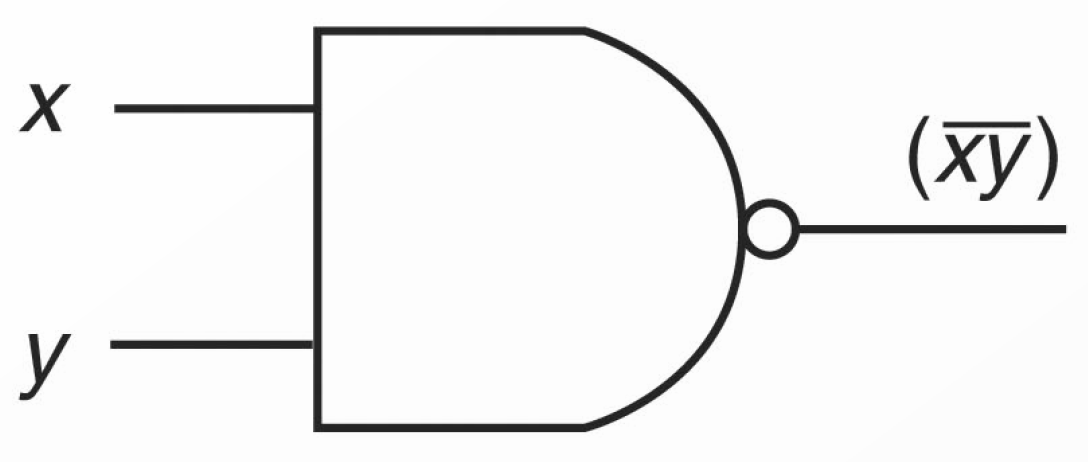
\includegraphics[width=4cm]{img/gates-nand.png} &
\begin{tabular}{|m{1cm}|m{1cm}|m{1cm}|m{0.1cm}}
\cline{1-3} $x$ & $y$ & $\overline{x \wedge y}$ &\\[1em]
\cline{1-3} 0 & 0 & 1 &\\[0.3em]
0 & 1 & 1 &\\
1 & 0 & 1 &\\
1 & 1 & 0 &\\[0.3em]
\cline{1-3}
\end{tabular}
& \\
\end{tabular}

\bigskip
%%%%%%%%%%%%%%%%%%%%%%%%%%
\subsection{Bramka XOR}
\index{bramka!XOR}

\begin{tabular}{m{6cm}m{7cm}m{0.1cm}}
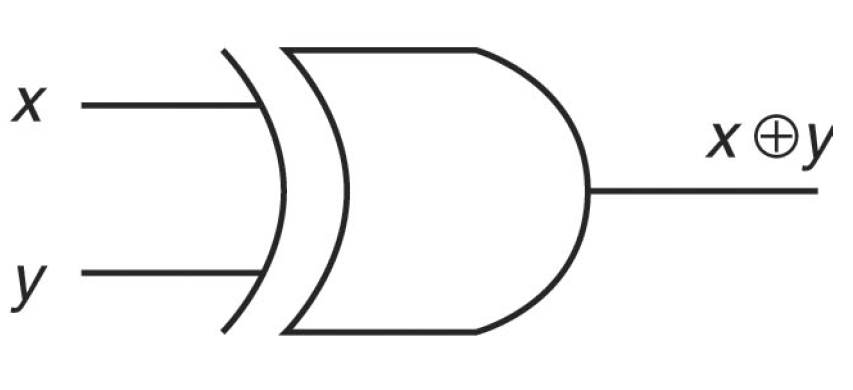
\includegraphics[width=4cm]{img/gates-xor.png} &
\begin{tabular}{|m{1cm}|m{1cm}|m{1cm}|m{0.1cm}}
\cline{1-3} $x$ & $y$ & $x \underline{\vee} y$ &\\[1em]
\cline{1-3} 0 & 0 & 0 &\\[0.3em]
0 & 1 & 1 &\\
1 & 0 & 1 &\\
1 & 1 & 0 &\\[0.3em]
\cline{1-3}
\end{tabular}
& \\
\end{tabular}


\chapter{Cia�o liczb zespolonych}

\medskip

Literatura do tego dzia�u: \cite{przybylo} - 2, \cite{ptak} - 3.3, \cite{kostrykin1} - 5.1\newline
Zadania do teog dzia�u: \cite{krysicki1} - 8.1, \cite{przybylo} - 2, \cite{ptak} - 3

\begin{definicja}
Cia�em \textbf{\emph{liczb zespolonych}}\label{def:liczby_zespolone}\label{def:liczba_zespolona} nazywamy cia�o (Def. \ref{def:cialo}, str. \pageref{def:cialo}) $(C, \oplus, \odot)$, w kt�rym $C = \mathbb{R} \times \mathbb{R}$, a dzia�ania $\oplus$ oraz $\odot$ s� okre�lone nast�puj�co:
\begin{center}
\begin{enumerate}
\item $\forall a, b, c, d \in \mathbb{R} \colon \qquad (a, b) \oplus (c, d) = (a + b, c + d)$
\item $\forall a, b, c, d \in \mathbb{R} \colon \qquad (a, b) \odot (c, d) = (ac - bd, ad + bc)$
\end{enumerate}
\end{center}
\cite[Rozdzia� 2]{przybylo}
\end{definicja}

\bigskip

W�a�ciwo�ci:
\begin{itemize}
\item elementem neutralnym (Def. \ref{def:element_neutralny}, str. \pageref{def:element_neutralny}) dzia�ania $\oplus$ jest liczba $\mathbf{(0,0)}$  
\item elementem neutralnym dzia�ania $\odot$ jest liczba $\mathbf{(1,0)}$
\item elementem przeciwnym (Def. \ref{def:element_przeciwny}, str. \pageref{def:element_przeciwny}) do liczby $(a, b)$ jest liczba
\[
-(a,b) = (-a, -b)
\]
\item elementem odwrotnym (Def. \ref{def:element_odwrotny}, str. \pageref{def:element_odwrotny}) do liczby $(a, b)$ jest liczba 
\[
(a,b)^{-1} = \left(\dfrac{a}{a^2 + b^2}, \dfrac{-b}{a^2 + b^2} \right)
\]
\end{itemize}

\bigskip
\begin{definicja}
\textbf{\emph{Cz�ci� rzeczywist�}}\label{def:czesc_rzeczywista} liczby zespolonej $z = (a, b)$ nazywamy liczb� rzeczywist� $a$ i oznaczamy
\[
Re \: z \quad = \quad a
\]
\end{definicja}

\medskip

\begin{definicja}
\textbf{\emph{Cz�ci� urojon�}}\label{def:czesc_urojona} liczby zespolonej $z = (a, b)$ nazywamy liczb� rzeczywist� $b$ i oznaczamy
\[
Im \: z \quad = \quad b
\]
\end{definicja}

\bigskip

\begin{definicja}
\textbf{\emph{Odejmowaniem}} liczb zespolonych nazywamy dodawanie pierwszego argumentu dzia�ania i elementu przeciwnego do drugiego argumentu dzia�ania.
\[
(a, b) \oplus -(c, d)
\]

\smallskip
co oznaczamy
\[
(a, b) \ominus (c, d)
\]
\end{definicja}

\bigskip
Liczba $(x, y)$ jest wynikiem odejmowania $(a, b) \ominus (c, d)$, gdy:
\[
\begin{array}{rcl}
(a, b) \ominus (c, d) & = & (x, y) \\ 
(a, b) \oplus -(c, d) & = & (x, y) \\
(a, b) \oplus (-c, -d) & = & (x, y)
\end{array}
\]

\medskip

Z definicji dodawania i r�wno�ci liczb zespolonych wynika, �e $a - c = x$ i $b - d = y$, st�d
\[
(a, b) \ominus (c, d) = (a - c, b -d)
\]

\bigskip
\begin{definicja}
\textbf{\emph{Dzieleniem}} liczb zespolonych nazywamy mno�enie pierwszego argumentu i elementu odwrotnego do drugiego argumentu dzia�ania.
\[
(a,b) \odot (c, d)^{-1}
\]
\smallskip
co oznaczamy
\[
\cdot\dfrac{(a,b)}{(c,d)}
\]
\end{definicja}

\bigskip
Lizcba $(x, y)$ jest wynikiem dzielenia $\cdot\dfrac{(a,b)}{(c,d)}$, gdy:
\[
\begin{array}{rcl}
\cdot\dfrac{(a,b)}{(c,d)} & = & (x, y) \vspace{0.2cm} \\
(a,b) \odot (c, d)^{-1} & = & (x, y) \vspace{0.2cm} \\
(a,b) \odot \left(\dfrac{c}{c^2 + d^2}, \dfrac{-d}{c^2 + d^2} \right) &=& (x,y)
\end{array}
\]

\medskip
Z definicji mno�enia i r�wno�ci liczb zespolonych wynika, �e:
\[
\left\{
\begin{array}{rlc}
a \cdot \dfrac{c}{c^2 + d^2} - b \cdot \dfrac{-d}{c^2 + d^2} &=& x
\vspace{0.5cm}
\\

a \cdot \dfrac{-d}{c^2 + d^2} + b \cdot \dfrac{c}{c^2 + d^2} &=& y
\end{array}
\right.
\]

\smallskip
st�d
\[
\cdot\dfrac{(a,b)}{(c,d)} = 
\left(
\dfrac{ac +bd}{c^2 + d^2},
\dfrac{bc -ad}{c^2 + d^2}
\right)
\]

\bigskip
%%%%%%%%%%%%%%%%%%%%%%%%%%%%%%%%%%%%
\section{Interpretacja geometryczna}

\medskip
Liczby zespolone i dzia�ania na nich mo�na interpretowa� geometrycznie. Wykorzystuj�c twierdzenie z geometrii analitycznej o istnieniu wzajemnie jednoznacznej odpowiednio�ci mi�dzy punktami p�aszczyzny i uporz�dkowanymi parami ortokartezja�skich wsp�rz�dnych punktu b�dziemy \textbf{\emph{liczb� zespolon�}} $\mathbf{(a, b)}$ interpretowa� jako \textbf{\emph{punkt}} o wsp�rz�dnych $\mathbf{a}$ i $\mathbf{b}$. Ka�dej wi�c liczbie zespolonej odpowiada dok�adnie jeden punkt p�aszczyzny, zwanej wtedy \textbf{\emph{p�aszczyzn� zespolon�}}.

\smallskip
Osie uk�adu nazywa� b�dziemy
\begin{itemize}
\item \textbf{\emph{osi� rzeczywist�}}\label{def:os_rzeczywista} - o�, na kt�rej le�� punkty odpowiadaj�ce liczbom zespolonym o cz�ci urojonej (Def. \ref{def:czesc_urojona}, str. \pageref{def:czesc_urojona}) r�wnej zeru
\item \textbf{\emph{osi� urojon�}}\label{os_urojona} - o�, na kt�rej le�� punkty odpowiadaj�ce liczbom zespolonym o cz�ci rzeczywistej (Def. \ref{def:czesc_rzeczywista}, str. \pageref{def:czesc_rzeczywista}) r�wnej zeru
\end{itemize}

\medskip
Analogicznie jak to czynili�my w uk�adzie ortokartezja�skim na p�aszczy�nie euklidesowej punktowi $z = a + bi$ b�dziemy przypisywa� wektor wodz�cy punktu, oznaczany tak�e przez $z$
\[
z = a \cdot \mathbf{1} + b \cdot i
\]
\smallskip
gdzie przez $\mathbf{1}$ oznaczyli�my wersor osi rzeczywistej, a przez $i$ wersor osi urojonej.
\cite[Rozdzia� 1.2]{trajdos}

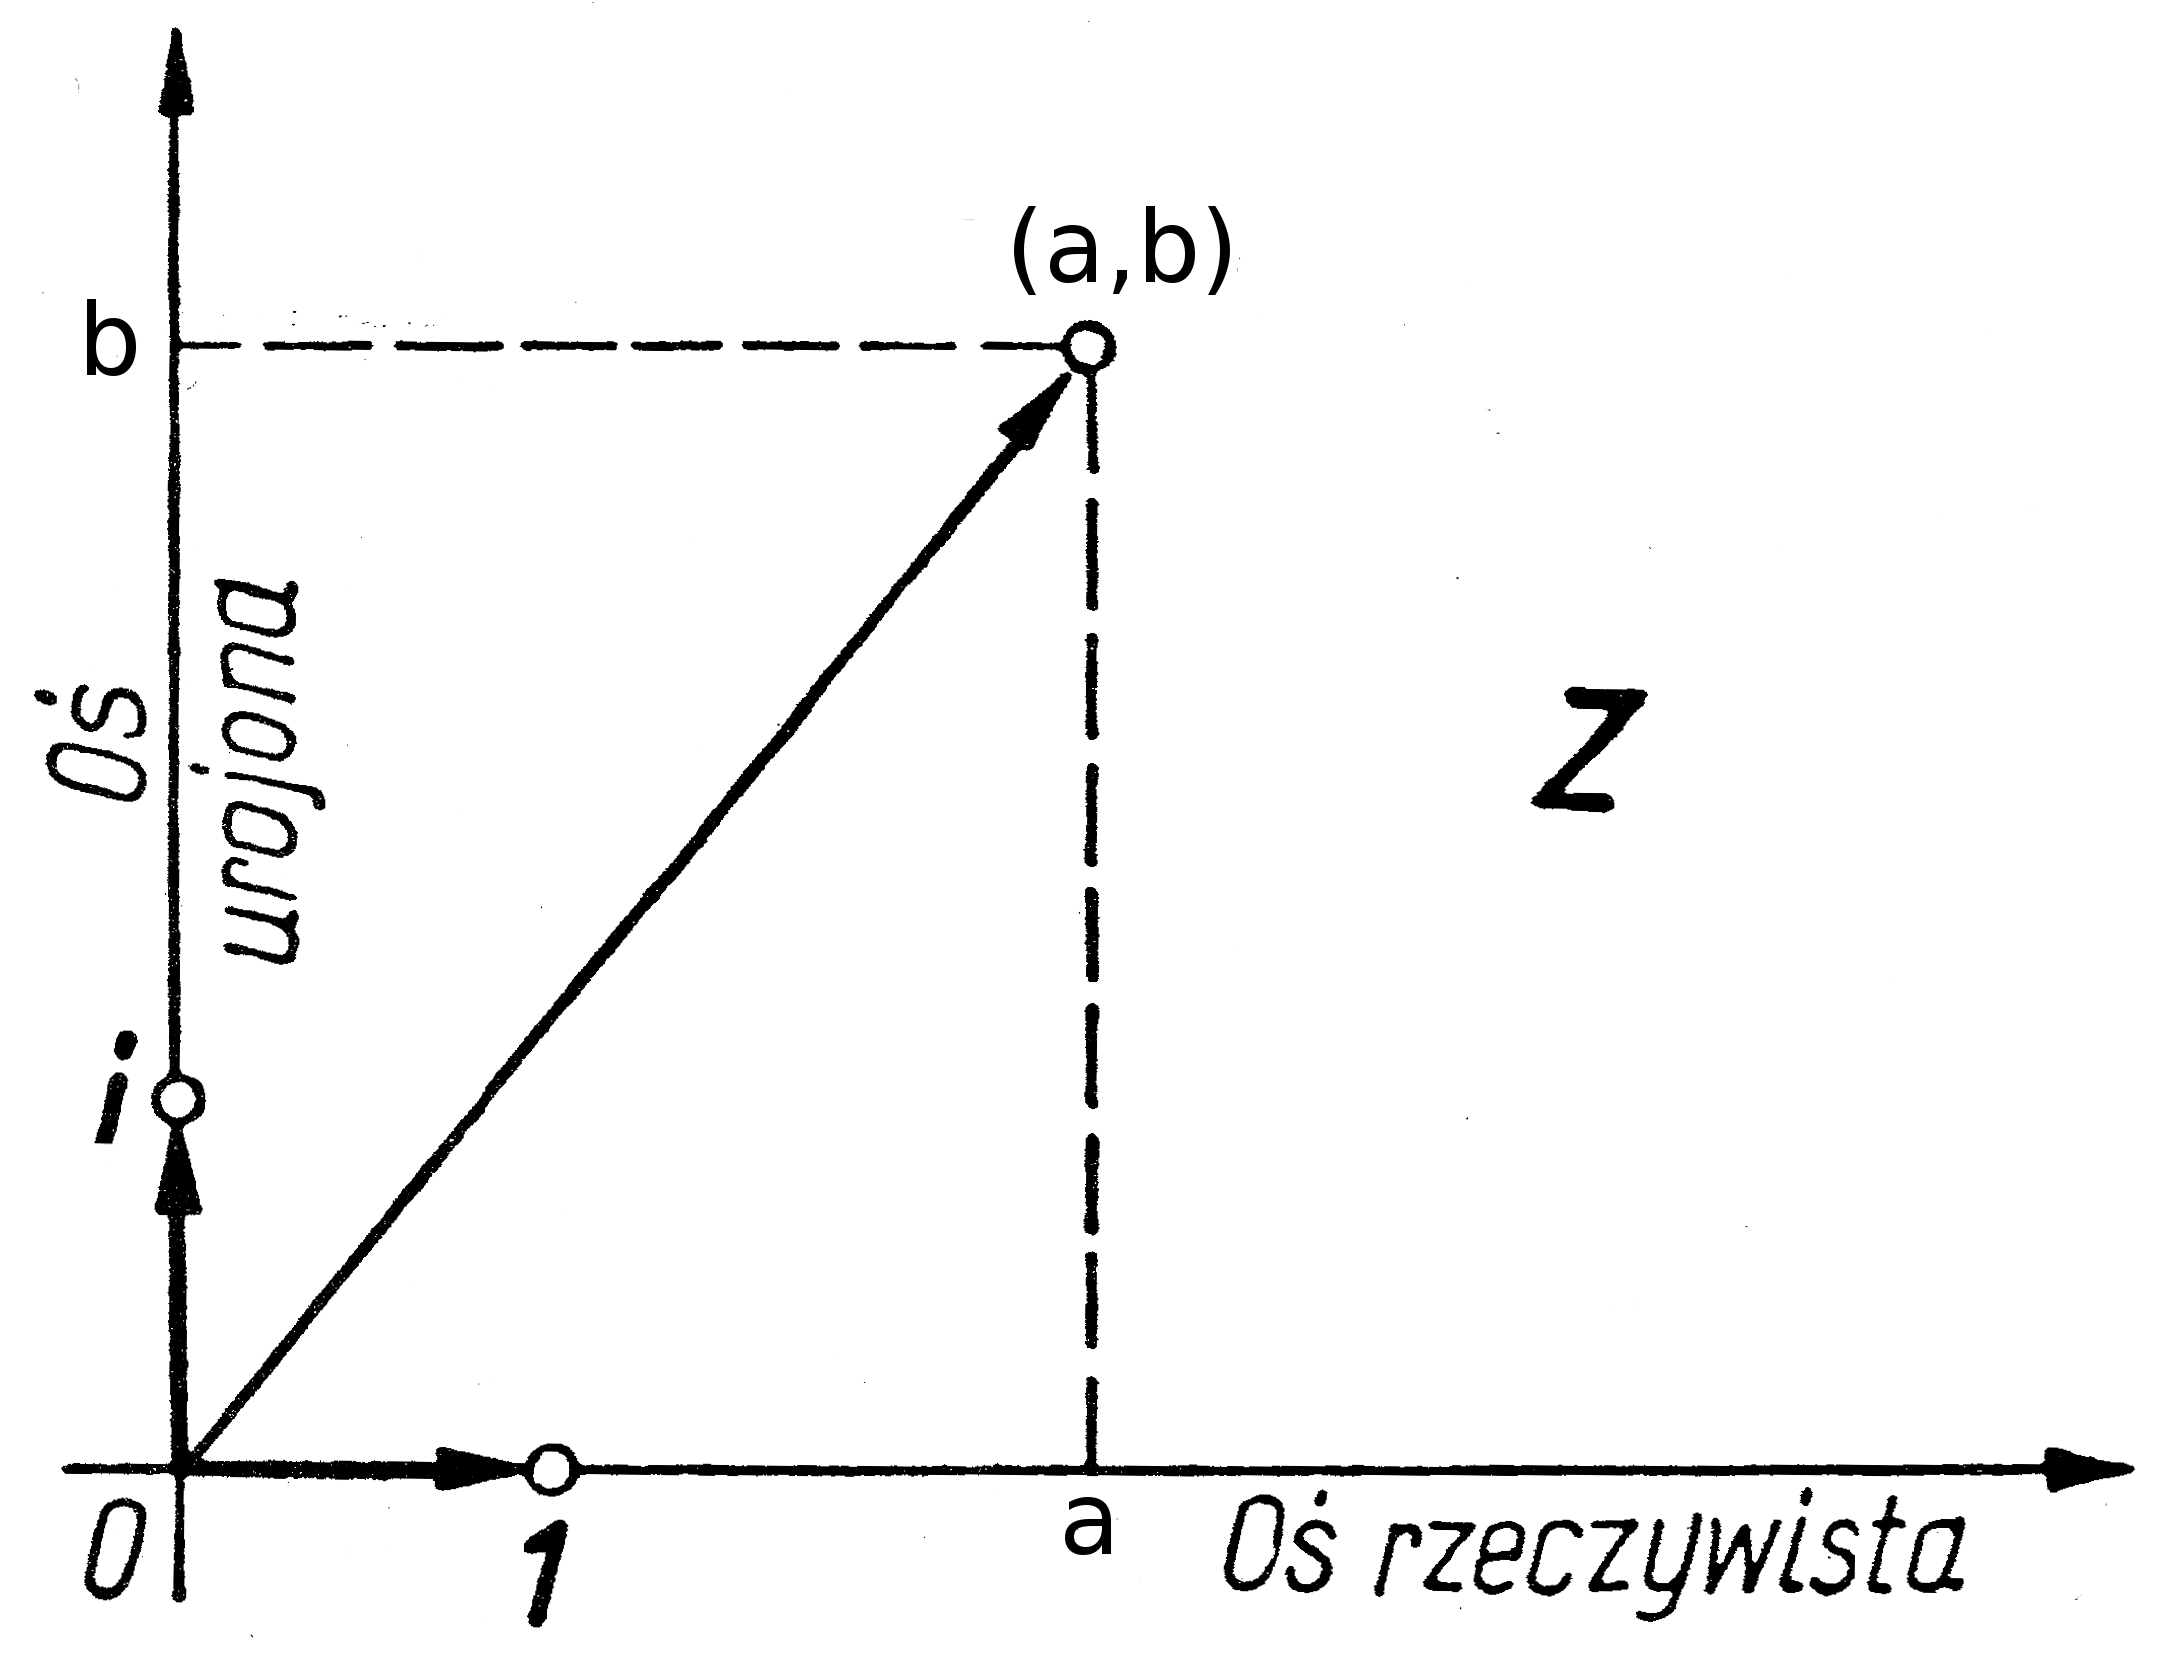
\includegraphics[scale=1.5]{img/zespolone-plaszczyzna_zespolona.png}

\bigskip
%%%%%%%%%%%%%%%%%%%%%%%%%%%%%
\section{Posta� algebraiczna}

\medskip

\begin{definicja}
Par� $(0, 1)$ oznaczamy symbolem $i$ oraz nazywamy \textbf{\emph{jednostk� urojon�}}\label{def:jednostka_urojona}.
\cite[Rozdzia� 2]{przybylo}
\end{definicja}

\bigskip

\begin{definicja}
Ka�d� liczb� zespolon� $(a, b)$ mo�na zapisa� w postaci $\mathbf{z = a + b\mathit{i}}$ (gdzie $i$ to jednostka urojona). Zapis taki nazywamy \textbf{\emph{postaci� algebraiczn�}}\label{def:postac_algebraiczna} liczby zespolonej.
\cite[Rozdzia� 2]{przybylo}
\end{definicja}

\bigskip
%%%%%%%%%%%%%%%%%%%%%%
\subsection{Dodawanie i odejmowanie}
\medskip
Dodawanie dw�ch liczb $z_1, z_2 \in \mathbb{C}$ postaci $z_1 = a_1 + b_1i$ oraz $z_2 = a_2 + b_2i$ mo�emy zapisa� w nast�puj�cy spos�b
\[
z_1 \oplus z_2 = \left( a_1 + a_2 \right) + \left( b_1 + b_2 \right)i
\]

\smallskip
a odejmowanie
\[
z_1 \ominus z_2 = \left( a_1 - a_2 \right) + \left( b_1 - b_2 \right)i
\]

\medskip
Dodawanie liczb zespolonych interpretujemy geometrycznie jako dodawanie przyporz�dkowanych im wektor�w, za� odejmowanie jako odejmowanie wektor�w
\cite[Rozdzia� 1.2]{trajdos}

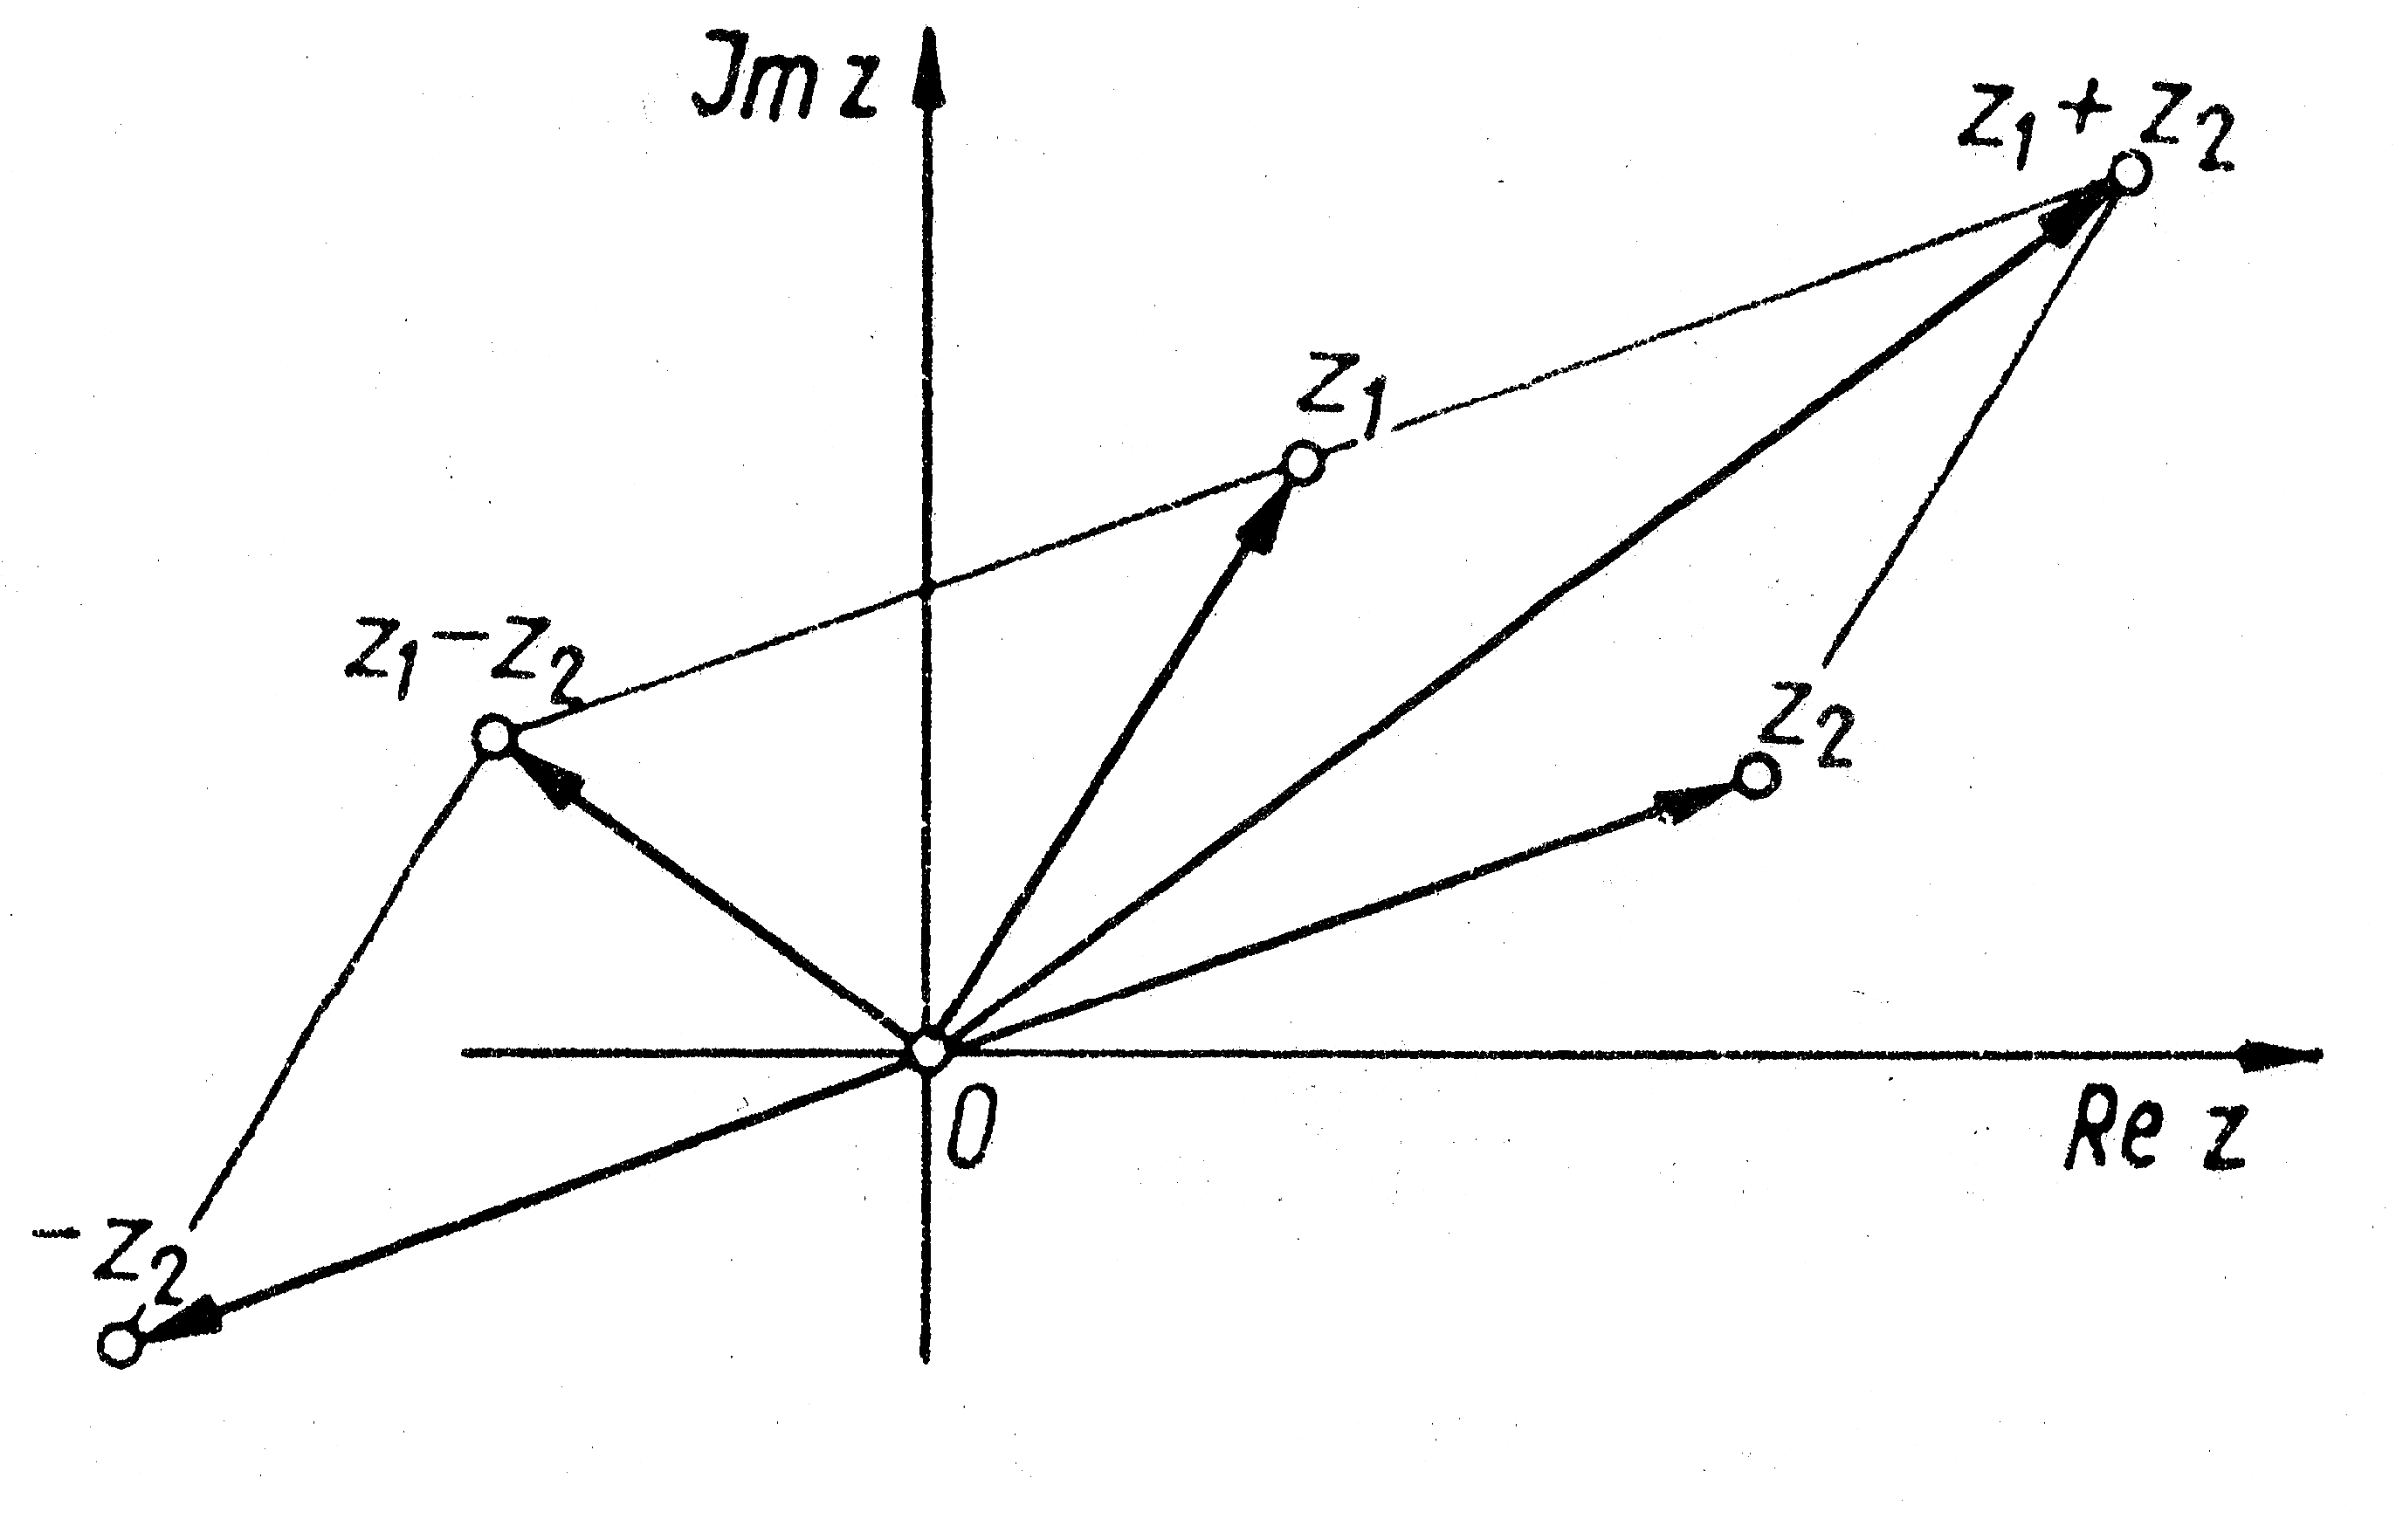
\includegraphics[scale=1.5]{img/zespolone-dodawanie_odejmowanie.png}

\bigskip
%%%%%%%%%%%%%%%%%%%%%%
\subsection{Mno�enie}
\medskip
Mno�enie dw�ch liczb $z_1, z_2 \in \mathbb{C}$ postaci $z_1 = a_1 + b_1i$ oraz $z_2 = a_2 + b_2i$ mo�emy zapisa� w nast�puj�cy spos�b
\[
z_1 \odot z_2 = \left(a_1a_2 - b_1b_2\right) + \left(a_1b_2 + b_1a_2\right)i 
\]

\bigskip
%%%%%%%%%%%%%%%%%%%%%%
\subsection{Dzielenie}
\medskip
Dzielenie dw�ch liczb $z_1, z_2 \in \mathbb{C}$ postaci $z_1 = a_1 + b_1i$ oraz $z_2 = a_2 + b_2i$ mo�emy zapisa� w nast�puj�cy spos�b
\[
\cdot\dfrac{z_1}{z_2} = \dfrac{a_1a_2 + b_1b_2}{a_2^2 + b_2^2} + \dfrac{b_1a_2 - a_1b_2}{a_2^2 + b_2^2}i 
\]

\bigskip
%%%%%%%%%%%%%%%%%%%%%%
\section{Modu� liczby zespolonej}
\medskip
\begin{definicja}
\textbf{\emph{Modu�em}}\label{def:modul_liczby_zespolonej} liczby zespolonej $z = a + bi$ nazywamy rzeczywist� liczb� nieujemn�
\[
|z| \quad = \quad \sqrt{a^2 + b^2}
\]
\end{definicja}
\medskip
Modu� liczby zespolonej interpretujemy geometrycznie jako d�ugo�� wektora wodz�cego punktu odpowiadaj�cego tej liczbie i oznaczamy $r$
\[
r \quad = \quad |z|
\]

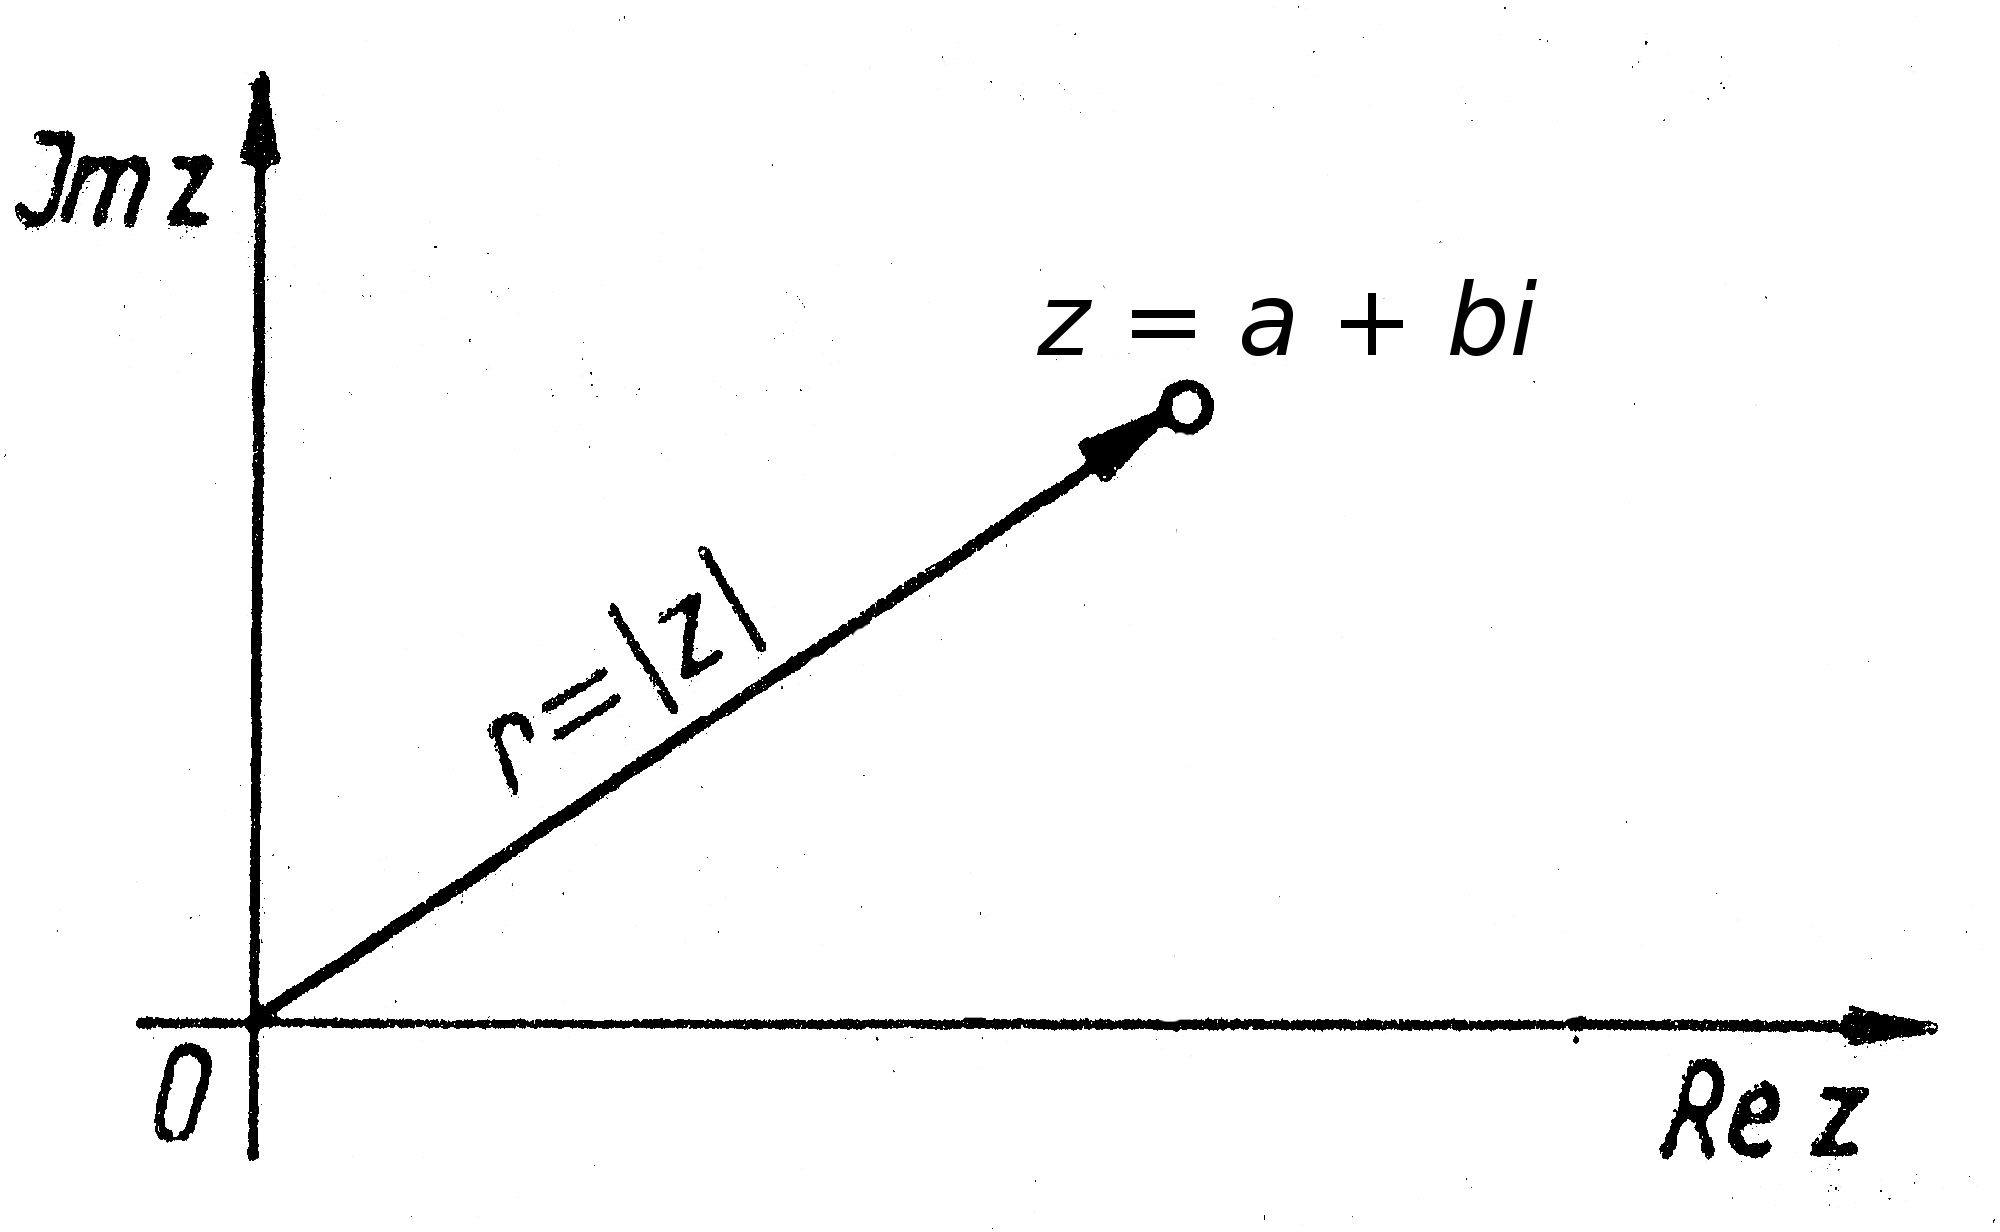
\includegraphics[scale=1.5]{img/zespolone-modul.png}

\bigskip
%%%%%%%%%%%%%%%%%%%%%%
\section{Liczba zespolona sprz�ona}
\medskip
\begin{definicja}
\textbf{\emph{Liczb� sprz�on�}}\label{def:liczba_zespolona_sprzezona} z~liczb� 

\[
z \; = \; a + bi
\]

\noindent nazywamy liczb� 

\[
a - bi
\]

\noindent i~oznaczamy $\overline{z}$

\[
\overline{z} \; = \; a - bi
\]
\cite[Rozdzia� 1.1]{trajdos}
\end{definicja}

\medskip

\begin{definicja}
Dwie liczby, z kt�rach jedna jest sprz�ona z drug�, nazywamy \textbf{\emph{liczbami sprz�onymi}}.
\end{definicja}

\medskip
W�asno�ci:
\begin{itemize}
\item Liczby sprz�one maj� r�wne modu�y
\[
|z| \quad = \quad \left|\overline{z}\right|
\]
\item Ilocznyn liczb sprz�onych jest r�wny kwadratowi ich wsp�lnego modu�u
\[
z \cdot \overline{z} \quad = \quad |z|^2
\] 
\end{itemize}

\medskip
Geometrycznie liczba sprz�ona z liczb� $z$ jest symetrycznym odbiciem wzgl�dem osi rzeczywistej (Def. \ref{def:os_rzeczywista}, str. \pageref{def:os_rzeczywista}).

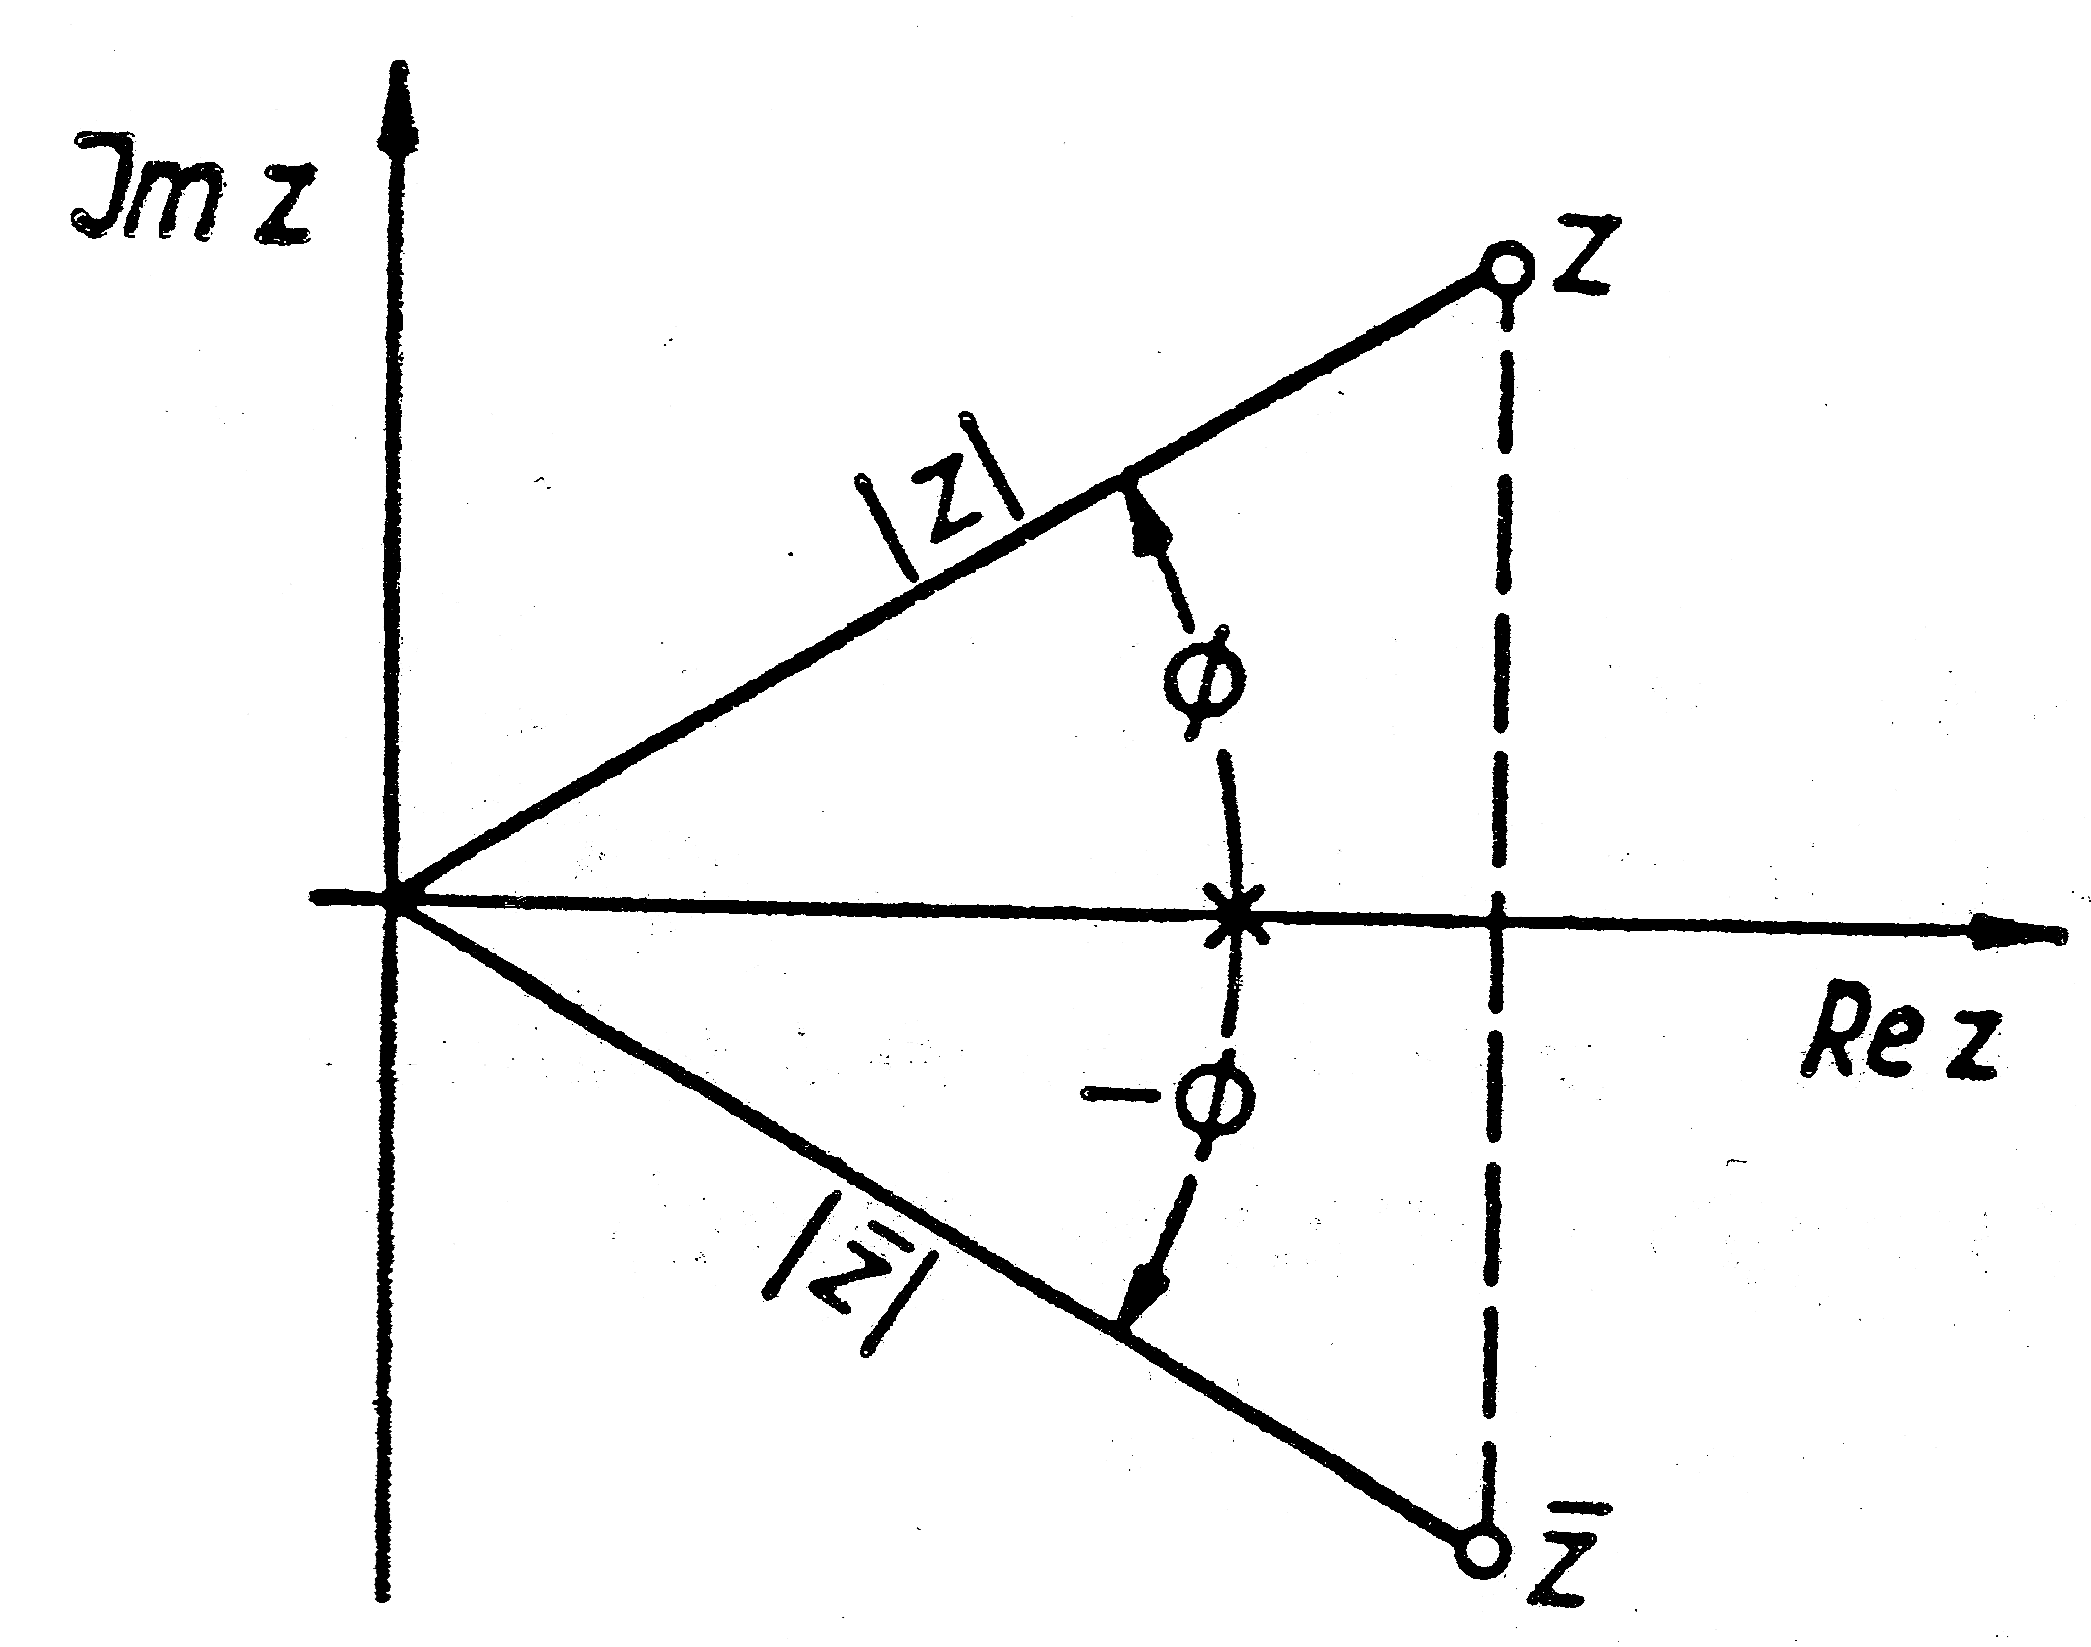
\includegraphics[scale=1.5]{img/zespolone-liczba_sprzezona.png}

\bigskip
%%%%%%%%%%%%%%%%%%%%%%
\section{Posta� trygonometryczna}
\medskip


\bigskip
%%%%%%%%%%%%%%%%%%%%%%
\subsection{Argument liczby zespolonej}
\medskip
\begin{definicja}
\textbf{\emph{Argumentem}}\label{def:argument_liczby_zespolonej} liczby zespolonej $z = a + bi \: \neq \mathbf{0}$ nazywamy ka�d� liczb� rzeczywist� $\varphi$ spe�niaj�c� warunki
\[
\left\{
\begin{array}{rcl}
cos\: \varphi &=& \dfrac{a}{|z|} \\
sin\: \varphi &=& \dfrac{b}{|z|}
\end{array}
\right.
\]
gdzie $|z|$ jest modu�em (Def. \ref{def:modul_liczby_zespolonej}, str. \pageref{def:modul_liczby_zespolonej}) liczby zespolonej $z$.
\medskip
Argument liczby zespolonej $z$ oznaczamy
\[
Arg \: z
\]
\cite[Rozdzia� 1.2]{trajdos}
\end{definicja}

\medskip
\begin{definicja}
\textbf{\emph{Argumentem g��wnym}} liczby zespolonej $z$ nazywamy ten sposr�d argument�w liczby zespolonej $z$, kt�ry nale�y do przedzia�u $\langle 0, 2\pi)$ i oznaczamy
\[
arg \: z
\]
\cite[Rozdzia� 1.2]{trajdos}
\end{definicja}

\medskip
Pomi�dzy argumentem g��wny a argumentem liczby zespolonej $z$ zachodzi zale�no��
\[
Arg \: z \quad = \quad arg \: z + 2k\pi, \qquad k = 0, \pm1, \ldots
\]
\medskip

Dla liczby $(0, 0)$ nie okre�la si� argumentu.

\medskip
Geometrycznie, argument liczby zespolonej jest miar� wzgl�dn� k�ta, jaki tworzy wektor wodz�cy punktu $z$ z osi� rzeczywist� (Def. \ref{def:os_rzeczywista}, str. \pageref{def:os_rzeczywista}).

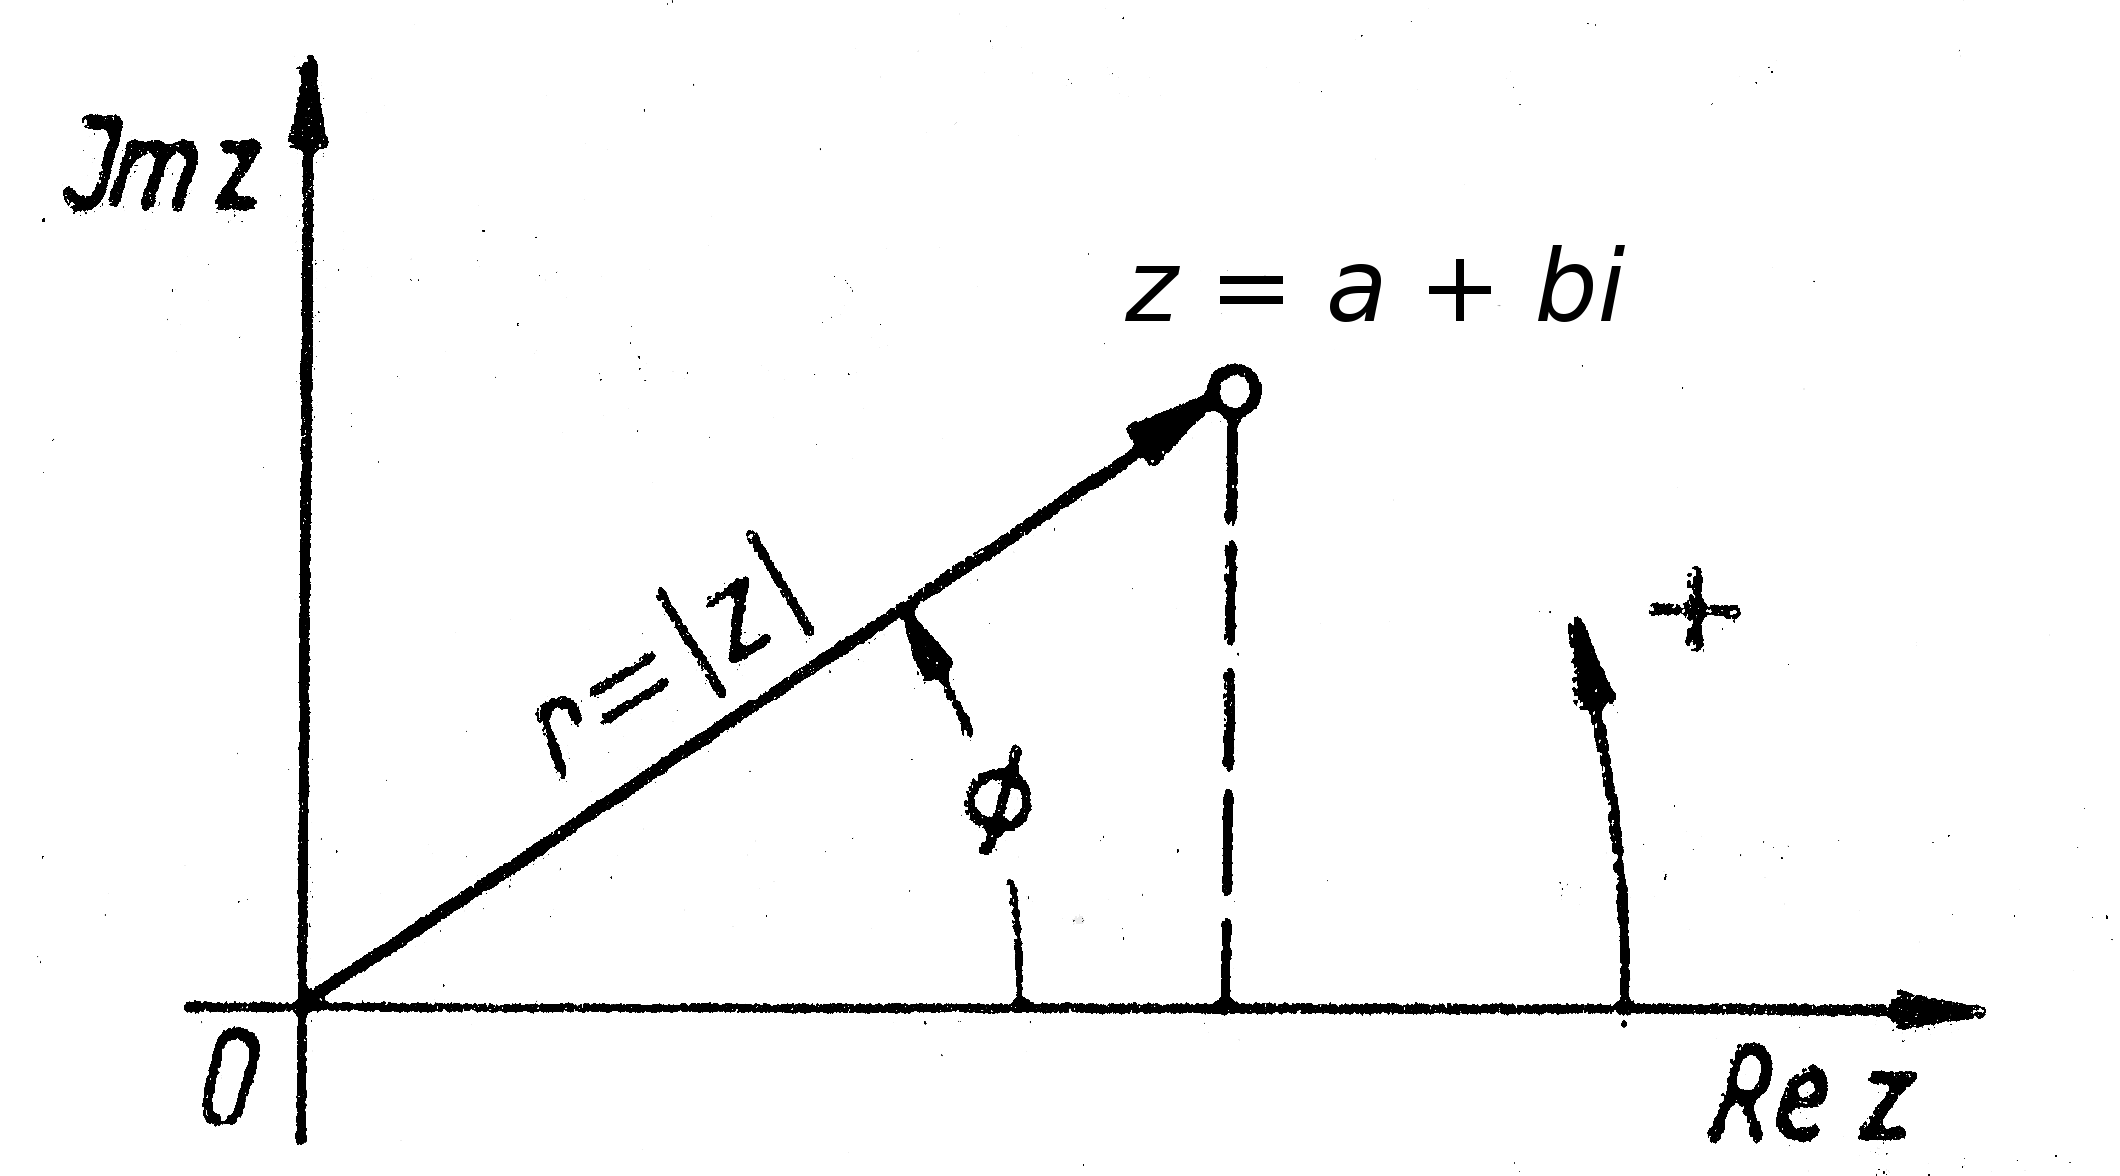
\includegraphics[scale=1.5]{img/zespolone-argument.png}

\bigskip
%%%%%%%%%%%%%%%%%%%%%%
\subsection{Posta� trygonometryczna liczby zespolonej}
\medskip
\begin{definicja}
Ka�d� liczb� zespolon� mo�na zapisa� w postaci
\[
r \: \left( cos \: \varphi + i \: sin \: \varphi \right)
\]
zwanej \textbf{\emph{postaci� trygonometryczn�}} liczby zespolonej. Czynnik $r$ jest modu�em (Def. \ref{def:modul_liczby_zespolonej}, str. \pageref{def:modul_liczby_zespolonej}) liczby za� $\varphi$ jest dowolnym jej argumentem (Def. \ref{def:argument_liczby_zespolonej}, str. \pageref{def:argument_liczby_zespolonej}).
\end{definicja}

\bigskip
%%%%%%%%%%%%%%%%%%%%%%
\subsection{Mno�enie}
\medskip
Niech b�d� dane dwie liczby zespolone w postaci trygonometrycznej
\[
z_1 \quad = \quad r_1 \: \left(cos \: \varphi_1 + i \: sin \: \varphi_1 \right)
\]
\[
z_2 \quad = \quad r_2 \: \left(cos \: \varphi_2 + i \: sin \: \varphi_2 \right)
\]

\medskip
Ich iloczynem b�dzie liczba
\[
\begin{array}{rcl}
z_1 z_2 & = &
\left[
r_1 \: \left(cos \: \varphi_1 + i \: sin \: \varphi_1 \right)
\right]
\left[
r_2 \: \left(cos \: \varphi_2 + i \: sin \: \varphi_2 \right)
\right] = \\
& = & r_1 r_2
\left[
\left(
cos \: \varphi_1
cos \: \varphi_2
-
sin \: \varphi_1
sin \: \varphi_2
\right)
+
i
\left(
cos \: \varphi_1
sin \: \varphi_2
+
sin \: \varphi_1
cos \: \varphi_2
\right)
\right]

\end{array}
\]

\medskip
lub po zastosowaniu wzor�w trygonometrycznych
\[
z_1 z_2 = r_1 r_2
\left[
cos \left(\varphi_1 + \varphi_2 \right)
+ i \:
sin \left(\varphi_1 + \varphi_2 \right)
\right]
\]

\medskip
Wnioski:
\begin{itemize}
\item modu� iloczynu liczb zespolonych jest r�wny iloczynowi ich modu��w
\[
\left| z_1 z_2 \right| = \left|z_1\right| \left|z_2\right|
\]
\item argument iloczynu liczb zespolonych jest r�wny sumie ich argument�w
\[
Arg \left(z_1 z_2 \right) = Arg \: z_1 + Arg \: z_2
\]
\end{itemize}

\bigskip
%%%%%%%%%%%%%%%%%%%%%%
\subsection{Dzielenie}
\medskip
Niech b�d� dane dwie liczby zespolone w postaci trygonometrycznej
\[
z_1 \quad = \quad r_1 \: \left(cos \: \varphi_1 + i \: sin \: \varphi_1 \right)
\]
\[
z_2 \quad = \quad r_2 \: \left(cos \: \varphi_2 + i \: sin \: \varphi_2 \right)
\]

\medskip
Ich ilorazem b�dzie liczba
\[
\begin{array}{rcl}
\cdot \dfrac{z_1}{z_2} & = &
\dfrac{
r_1 \: \left(cos \: \varphi_1 + i \: sin \: \varphi_1 \right)
}
{
r_2 \: \left(cos \: \varphi_2 + i \: sin \: \varphi_2 \right)
} = \vspace{0.5cm}\\
& = &
\dfrac{r_1}{r_2}
\dfrac{\left(cos \: \varphi_1 + i sin \: \varphi_1 \right) \left(cos \: \varphi_2 - i sin \: \varphi_2 \right)}{cos^2 \: \varphi_2 + cos^2 \: \varphi_2}

\end{array}
\]

\medskip
lub po zastosowaniu wzor�w trygonometrycznych
\[
\cdot \dfrac{z_1}{z_2} = \dfrac{r_1}{r_2}
\left[
cos \left(\varphi_1 - \varphi_2 \right)
+ i \:
sin \left(\varphi_1 - \varphi_2 \right)
\right]
\]

\medskip
Wnioski:
\begin{itemize}
\item modu� ilorazu liczb zespolonych jest r�wny ilorazowi ich modu��w
\[
\left| \cdot \dfrac{z_1}{z_2} \right| = \dfrac{\left|z_1\right|}{\left|z_2\right|}
\]
\item argument ilorazu liczb zespolonych jest r�wny r�nicy ich argument�w
\[
Arg \: \cdot \dfrac{z_1}{z_2} = Arg \: z_1 - Arg \: z_2
\]
\end{itemize}


\bigskip
%%%%%%%%%%%%%%%%%%%%%%
\subsection{Pot�gowanie}
\medskip
Niech b�dzie dana liczba zespolona w postaci trygonometrycznej
\[
z \quad = \quad r \: \left(cos \: \varphi + i \: sin \: \varphi\right)
\]

\medskip
Jej pot�g� o wyk�adniku naturalnym b�dzie
\[
z^n \quad = \quad r^n \: \left(cos \: n\varphi + i \: sin \: n\varphi\right)
\]
gdzie $n \in \mathbb{N}$

\bigskip
\subsubsection{Wyprowadzanie wzor�w trygonometrycznych}
Niech b�dzie dana liczba zespolona $z$ o module r�wnym 1 ($|z| = 1$)
\[
z \quad = \quad cos \: \varphi + i \: sin \: \varphi
\]
\medskip
Chcemy policzy� $z^2$. \linebreak
\medskip
Ze wzoru na pot�g� liczby zespolonej w postaci trygonometrycznej mamy
\[
z^2 \quad = \quad cos \: 2\varphi + i \: sin \: 2\varphi
\]
\medskip
Mo�emy tak�e skorzysta� z takiego r�wnania
\[
\begin{array}{rcl}
z^2 & = & \left(cos \: \varphi + i \: sin \: \varphi\right)^2 = \\
& = & cos^2 \: \varphi - sin^2 \: \varphi + i \: 2 \: sin \: \varphi cos \: \varphi
\end{array}
\]
\medskip
Z r�wno�ci liczb zespolonych wynika, �e
\[
\left\{
\begin{array}{rcl}
cos \: 2\varphi & = & cos^2 \: \varphi - sin^2 \: \varphi \\
sin \: 2\varphi & = & 2 \: sin \: \varphi cos \: \varphi
\end{array}
\right.
\]
\medskip
Wyprowadzili�my w ten spos�b wzory na $cos \: 2\varphi$ i $sin \: 2\varphi$.
W og�lno�ci, dla dowolnego $n$, otrzymyjemy wz�r Moivre'a.
\medskip
\begin{definicja}
\textbf{\emph{Wzorem Moivre'a}} nazywamy r�wnanie
\[
\left(
cos \: \varphi + i \: sin \: \varphi \right)^n
\quad 
=
\quad
cos\left(n\varphi\right) + i \: sin\left(n\varphi\right)
\]
\end{definicja}


\bigskip
%%%%%%%%%%%%%%%%%%%%%%
\subsection{Pierwiastkowanie}
\medskip
\begin{definicja}
Je�eli $z_0 = r_0\left(cos \: \varphi_0 + i \: sin \: \varphi_0\right) \: \neq \: 0$, przy czym $\varphi_0 = arg \: z_0$, to liczba $\omega = R \left(cos \: \psi + i \: sin \: \psi \right)$ jest \textbf{\emph{pierwiastkiem stopnia $n$}} z $z_0$ wtedy i tylko wtedy, gdy
\[
R^n \quad = \quad r_0
\]

oraz
\[
n \: \psi \quad = \quad \varphi_0 + 2k\pi
\]

gdzie $k$ jest liczb� ca�kowit�.
\cite[Rozdzia� 1.3]{trajdos}
\end{definicja}


\bigskip
St�d
\[
R \quad = \quad \sqrt[n]{r_0}
\]

oraz
\[
\psi \quad = \quad \dfrac{\varphi_0}{n} + \dfrac{2\pi}{n}k, \qquad k = 0, \pm1, \pm2, \ldots
\]

\bigskip
Wszystkie r�ne pierwiastki stopnia $n$ z liczby $z_0$ mo�na zapisa� wzorem
\[
\omega_k \quad = \quad \sqrt[n]{r_0}
\left[
  cos \left(
    \dfrac{\varphi_0}{n} + \dfrac{2\pi}{n}k
      \right)
  +
  i \:
  sin \left(
    \dfrac{\varphi_0}{n} + \dfrac{2\pi}{n}k
      \right)
\right]
\]

\bigskip
Na rysunku zosta�o przedstawionych $n$ pierwiastk�w stopnia $n$ liczby $z_0 \neq 0$. Odcinki przerywane ��cz�ce kolejne pierwiastki tworz� wielobok foremny wpisany w okr�g o promieniu $\sqrt[n]{r_0}$.

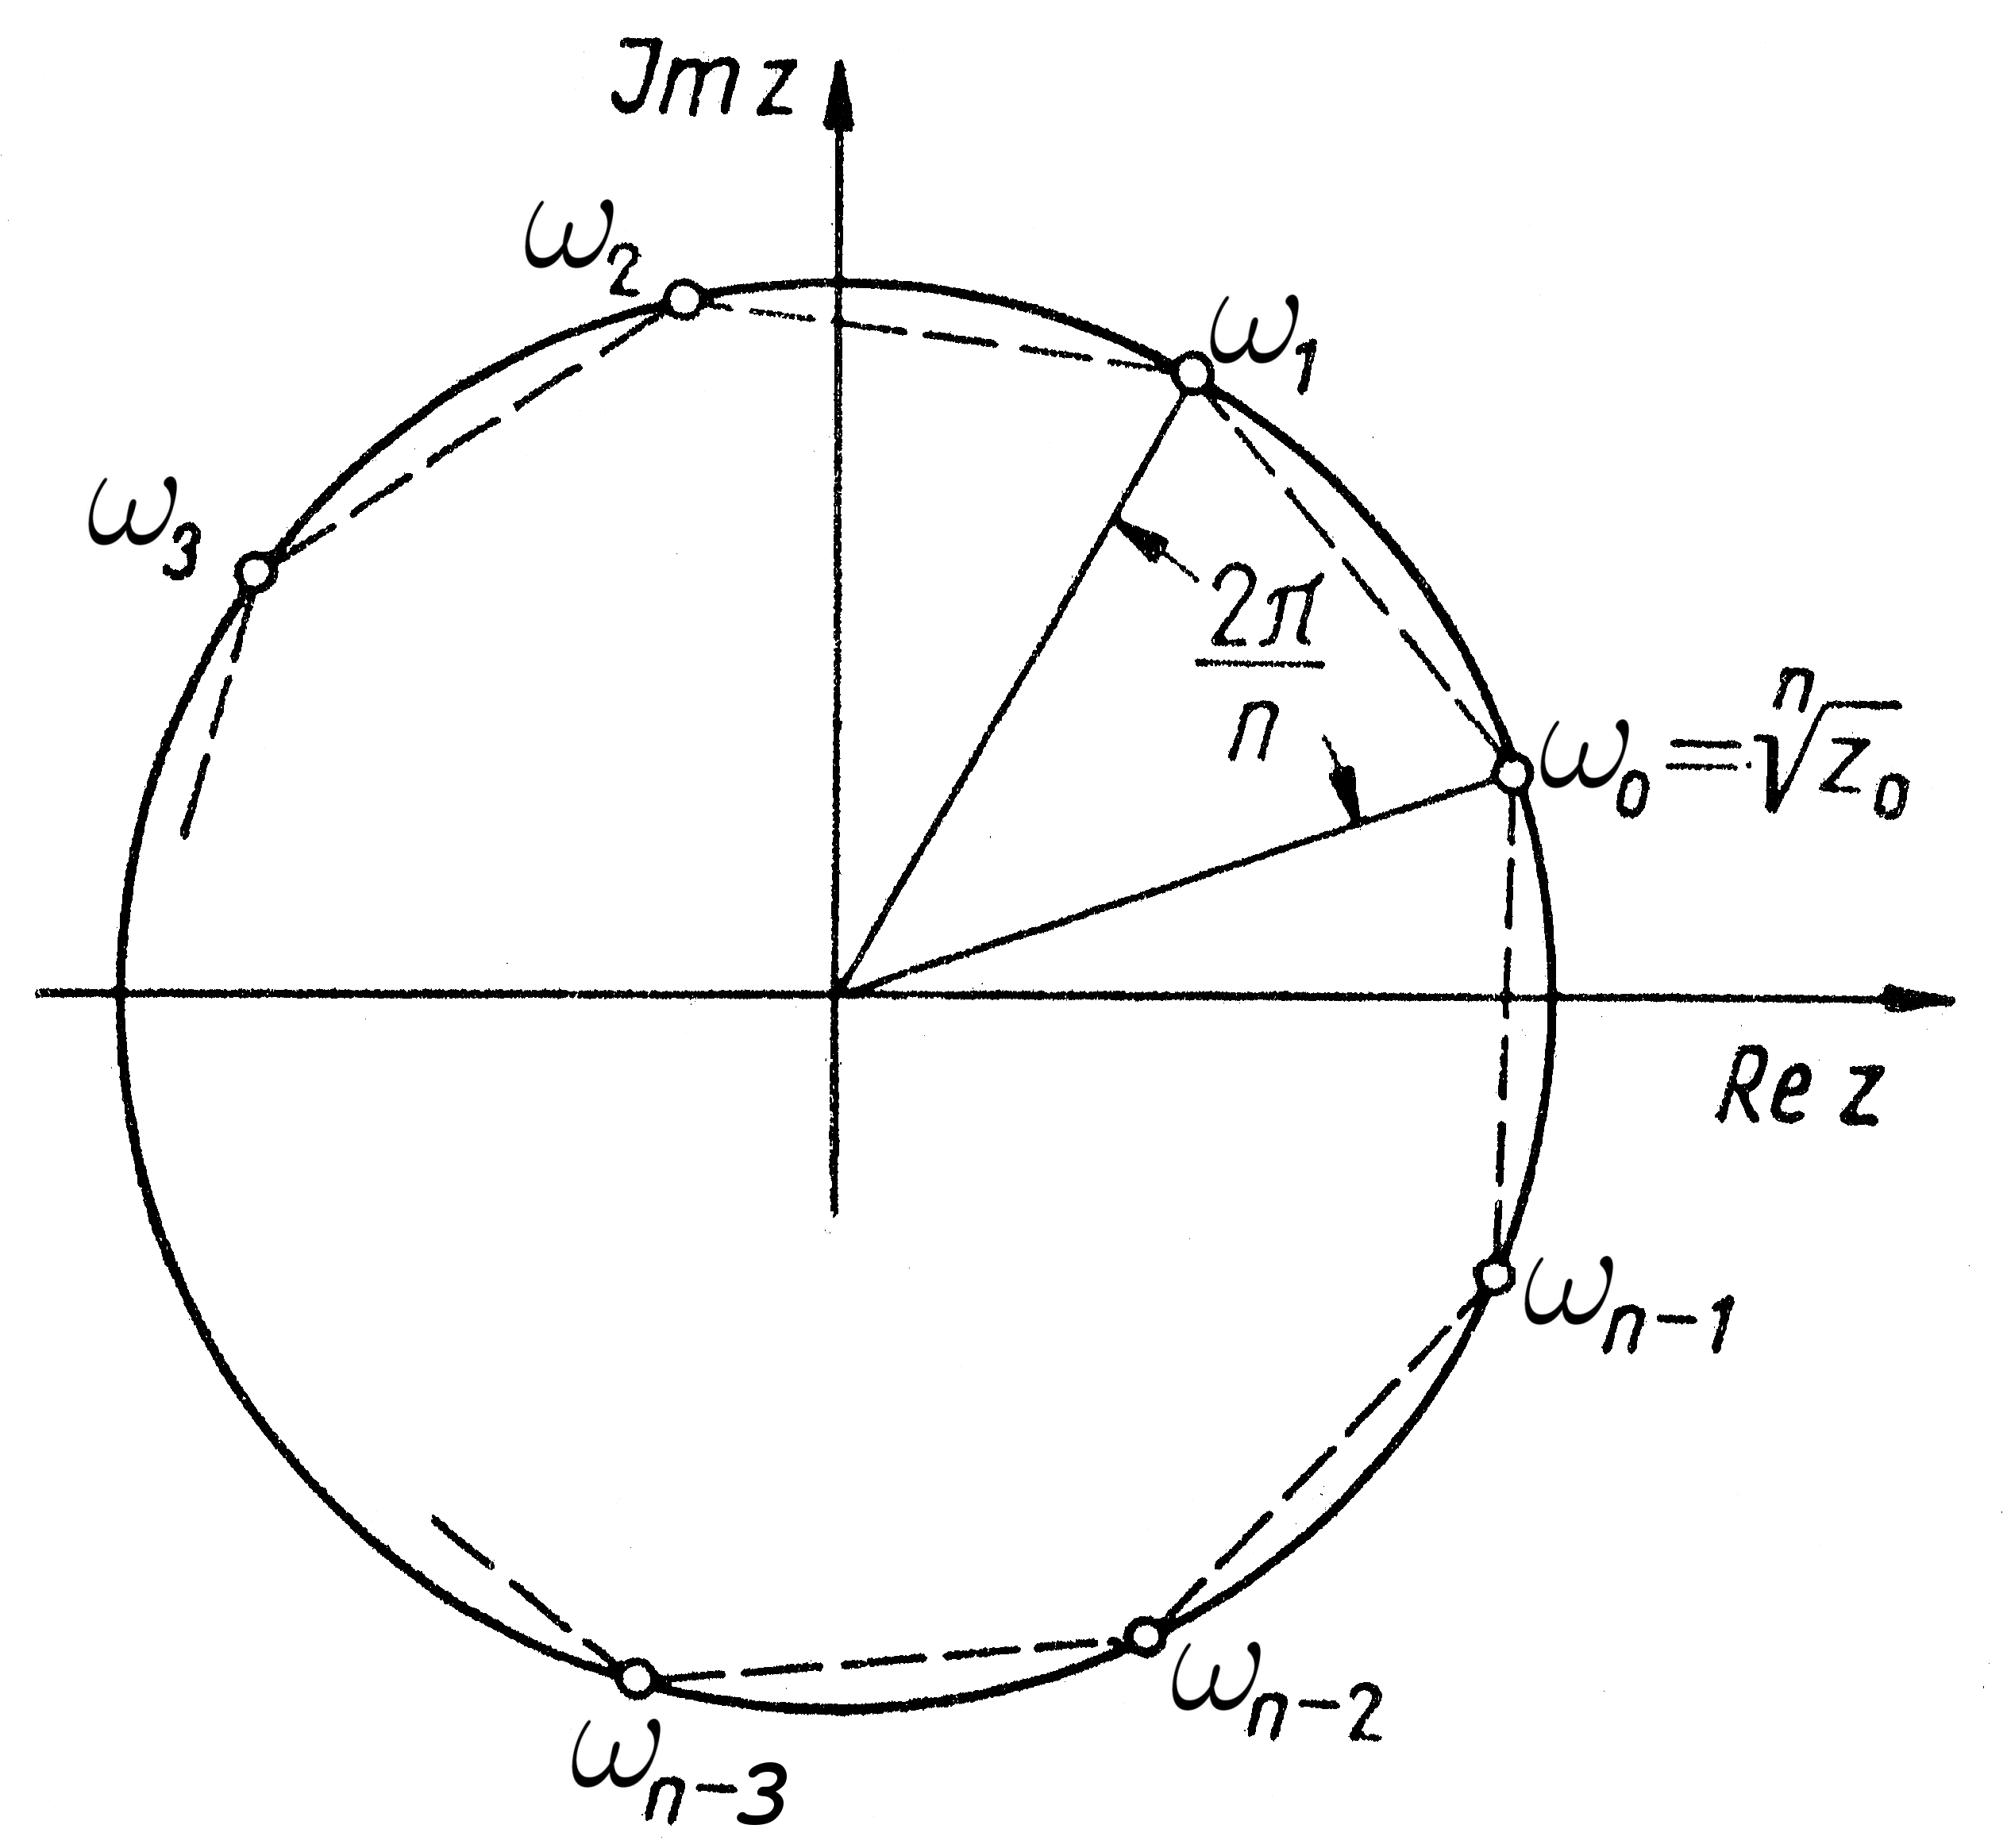
\includegraphics[scale=1.5]{img/zespolone-pierwiastkowanie.png}

\bigskip
%%%%%%%%%%%%%%%%%%%%%%
\section{Wz�r Eulera}
\medskip
\begin{definicja}
\label{def:wzor_eulera} Pot�g� $e^z$ o podstawie $e$ i wyk�adniku $z = a + bi$, nale��cym do cia�a liczb zespolonych, okre�lamy w spos�b nast�puj�cy
\[
\begin{array}{rcl}
e^{ib} & = & cos \: b + i \: sin \: b \\
e^z & = & e^a \: e^{ib}
\end{array}
\]
\end{definicja}

\medskip
Definicja \ref{def:wzor_eulera} wprowadza nowy symbol $e^{i\varphi}$ na oznaczenie liczby o module r�wnym $1$ i argumencie $\varphi$, mianowicie
\[
e^{i\varphi} = cos \: \varphi + i \: sin \: \varphi
\]

\smallskip

R�wno�� ta umo�liwia zapisanie dowolnej liczby zespolonej $a + ib = r \left( cos\: \varphi + i \: sin \: \varphi \right)$ w tzw. \textbf{\emph{postaci wyk�adniczej}}.
\[
r \: e^{i\varphi}
\]

\chapter{Wielomiany. Funkcje wymierne}

\section{Pier�cie� ca�kowity wielomian�w}

Niech
\begin{itemize}
\item $x$ oznacza \emph{zmienn� zespolon�}, tzn. zmienn� nale��c� do cia�a $\mathbb{C}$ liczb zespolonych,
\item $\mathbb{K}$ za� jedno z cia� liczbowych:
\begin{itemize}
\item $\mathbb{C}$ - liczb zespolonych lub
\item $\mathbb{R}$ - liczb rzeczywistych
\end{itemize}
\end{itemize}

\medskip
\begin{definicja}
\textbf{\emph{Wielomianem}}\label{def:wielomian} nad cia�em liczbowym $\mathbb{K}$ nazywamy funkcj� zmiennej zespolonej $x$, okre�lon� wzorem
\[
f(x) \; = \; a_n x^n + a_{n-1} x^{n-1} + \ldots + a_2 x^2 + a_1 x + a_0
\]
gdzie
\begin{itemize}
\item liczby $a_k$ nale�� do cia�a $\mathbb{K}$ i nazywane s� \textbf{\emph{wsp�czynnikami wielomianu}}\label{def:wspolczynniki_wielomianu} ($k \: = \: 1, 2, \ldots, n$)
\item $n$ jest liczb� ca�kowit� nieujemn�
\item $a_0$ nazywamy \textbf{\emph{wyrazem wolnym}}\label{def:wyraz_wolny_wielomianu}
\item je�eli $a_n \neq 0$, to liczb� $n$ nazywamy \textbf{\emph{stopniem wielomianu}}\label{def:stopien_wielomianu}.
\end{itemize}
\end{definicja}

\medskip
\begin{twierdzenie}\label{tw:rownosc_wielomianow}
Dwa wielomiany

\medskip

\begin{tabular}{rclc}
$f(x)$ & $=$ & $a_n x^n + \ldots + a_0$ & $a_n \neq 0$ \\
$g(x)$ & $=$ & $b_m x^m + \ldots + b_0$ & $b_m \neq 0$
\end{tabular}

\begin{itemize}
\item dla kt�rych $m \leq n$
\item kt�re w $n + 1$ r�nych punktach $x_0, x_1, \ldots, x_n$ przybieraj� r�wne warto�ci
\item s� tego samego stopnia
\item maj� odpowiednie wsp�czynniki r�wne
\end{itemize}

s� \textbf{identyczne}.

\end{twierdzenie}

\medskip

\begin{definicja}
\textbf{\emph{Pierwiastkiem}}\label{pierwiastek_wielomianu} niezerowego wielomianu $f(x)$ nazywamy liczb� $a$, gdy
\[
f(a) \; = \; 0
\]

Pierwiastek niezerowego wielomianu nazywamy tak�e
\begin{itemize}
\item \textbf{\emph{miejscem zerowym}}\label{def:miejsce_zerowe_wielomianu}
\item \textbf{\emph{zerem wielomianu}}\label{def:zero_wielomianu}
\end{itemize}
\end{definicja}

\medskip

\begin{twierdzenie}[B\'{e}zout]
Wielomian $f(x)$ naturalnego stopnia jest wtedy i tylko wtedy podzielny przez dwumian $x - a$, gdy liczba $a$ jest zerem tego wielomianu.
\end{twierdzenie}

\medskip

\begin{definicja}
\textbf{\emph{$k$-krotnym pierwiastkiem}}\label{def:k-krotny_pierwiastek_wielomianu} niezerowego wielomianu $f(x)$ nazywamy liczb� $a$ gdy $(x - a)^k$ jest dzielnikiem tego wielomianu, za� $(x - a)^{k+1}$ nie jest jego dzielnikiem.

Liczb� $k$ nazywamy \textbf{\emph{krotno�ci�}} tego pierwiastka.
\end{definicja}

\medskip

\cite[Rozdzia� 9.1]{trajdos}

\bigskip
%%%%%%%%%%%%%%%%%%%%%%%%%%%%%%%%%%%%%%%%%%%%%%%%%
\section{Wielomiany nad cia�em liczb zespolonych}
Niech $W_n(z)$ b�dzie wielomianem naturalnego stopnia $n$ o wsp�czynnikach rzeczywistych
\[
W_n \quad = \quad
a_n \: z^n
+ a_{n-1} \: z^{n-1}
+ \ldots
+ a_1 \: z
+ a_0
\]

gdzie
\[
a_i \in R \qquad i = 0, \: 1, \: \ldots, \: n
\]

\medskip
\begin{twierdzenie}
Je�eli $W_n(z)$ jest wielomianem o wsp�czynnikach rzeczywistych, to
\[
\overline{ W_n(z) } \quad = \quad W_n( \overline{z} )
\]
\cite[Rozdzia� 9.2]{trajdos}
\end{twierdzenie}

\medskip
\begin{twierdzenie}
Je�eli $a$ jest $k$-krotnym pierwiastkiem wielomianu $W_n(z)$, to liczba $\overline{a}$, sprz�ona z pierwiastkiem $a$, jest tak�e $k$-krotnym pierwiastkiem tego wielomianu.
\[
W_n(a) = 0 \qquad \Rightarrow \qquad W_n\left(\overline{a}\right) = 0
\]
\cite[Rozdzia� 9.2]{trajdos}
\end{twierdzenie}


\bigskip
%%%%%%%%%%%%%%%%%%%%%%%%%%%%%%%%%%
\section{Cia�o funkcji wymiernych}

\begin{definicja}
\textbf{\emph{Funkcj� wymiern�}}\label{def:funkcja_wymierna} nad cia�em liczbowym $\mathbb{K}$ nazywamy funkcj� zmiennej zespolonej $x$, okre�lon� wzorem postaci
\[
f(x) \; = \; \dfrac{P_n(x)}{Q_m(x)}, \qquad Q \neq 0
\]

gdzie $P_n(x)$ i $Q_m(x)$ s� wielomianami zmiennej zespolonej $x$ nad cia�em liczbowym $K$.

\medskip
Funkcj� wymiern� nazywamy
\begin{itemize}
\item \textbf{\emph{w�a�ciw�}}\label{def:funkcja_wymierna_wlasciwa} gdy $n < m$
\item \textbf{\emph{niew�a�ciw�}}\label{def:funkcja_wymierna_niewlasciwa}, gdy $m \geq n$
\end{itemize}

\end{definicja}

\medskip

\begin{twierdzenie}\label{tw:funkcja_wymierna_suma_wielomianu_i_funkcji_wymiernej_wlasciwej}
Ka�d� funkcj� wymiern� mo�na przedstawi� w postaci sumy wielomianu i funkcji wymiernej w�a�ciwej.
\[
\dfrac{P_p(x)}{Q_q(x)} \; = \; W_w(x) \: + \: \dfrac{R_r(x)}{Q_q(x)}
\]

przy czym
\begin{itemize}
\item $w = 0$ lub $w = p - q$ gdy $P_p(x)/Q_q(x)$ jest funkcj� wymiern� niew�a�ciw�
\item $r < q$
\end{itemize}
\end{twierdzenie}

\medskip

\cite[Rozdzia� 9.3]{trajdos}


\bigskip
%%%%%%%%%%%%%%%%%%%%%%%%%%
\subsection{U�amki proste}

\begin{definicja}
\textbf{\emph{U�amkiem prostym}}\label{def:ulamek_prosty} nad cia�em $\mathbb{K}$ nazywamy funkcj� wymiern� nad tym cia�em:
\[
\dfrac{P_n(x)}{\left[Q_m(x)\right]^n}, \qquad Q \neq 0
\]

przy czym
\begin{itemize}
\item $Q$ jest wielomianem \textbf{nierozk�adalnym} w tym ciele
\item $n < m$
\item $n$ jest liczb� naturaln� 
\end{itemize}

\end{definicja}

\bigskip

U�amki proste nad cia�em
\begin{itemize}
\item $\mathbb{C}$ liczb zespolonych maj� posta�
\[
\dfrac{A}{(x - a)^n}, \qquad \textnormal{ gdzie } A, a \textnormal{ - liczby zespolone}
\]
\item $\mathbb{R}$ liczb rzeczywistych maj� posta�
\begin{itemize}
\item u�amki proste pierwszego rodzaju\label{def:ulamek_prosty_pierwszego_rodzaju}
\[
\dfrac{A}{(x - a)^n}, \qquad \textnormal{ gdzie } A, a \textnormal{ - liczby rzeczywiste}
\]
\item u�amki proste drugiego rodzaju\label{def:ulamek_prosty_drugiego_rodzaju}
\[
\dfrac{Ax + B}{(x^2 + px + q)^n},
\begin{array}{c}
\textnormal{ gdzie } A, B, p, q \textnormal{ - liczby rzeczywiste}, \\ 
p^2 - 4q < 0
\end{array}
\]
\end{itemize}
\end{itemize}

\medskip

\begin{twierdzenie}\label{tw:o_rozkladzie_na_ulamki_proste}
\textbf{Ka�d� funkcj� wymiern� w�a�ciw�} (Def. \ref{def:funkcja_wymierna_wlasciwa}, str. \pageref{def:funkcja_wymierna_wlasciwa}) w ciele $\mathbb{C}$ liczb zespolonych ($\mathbb{R}$ liczb rzeczywistych) mo�na przedstawi� w postaci \textbf{sumy u�amk�w prostych}.

\medskip

Ka�demu czynnikowi w rozk�adzie jej \textbf{mianownika} typu
\begin{itemize}
\item $(x - a)^n$ (w ciele $\mathbb{C}$ i $\mathbb{R}$) odpowiada sk�adnik postaci
\[
\dfrac{A_n}{(x - a)^n} + \dfrac{A_{n-1}}{(x - a)^{n-1}} + \ldots + \dfrac{A_1}{x - a}
\]
\item $(x^2 + px + q)^n, \; p^2 - 4q < 0$ (w ciele $\mathbb{R}$) odpowiada sk�adnik postaci
\[
\dfrac{A_nx + B_n}{(x^2 + px + q)^n} + \dfrac{A_{n-1}x + B_{n-1}}{(x^2 + px + q)^{n-1}} + \ldots + \dfrac{A_1x + B_1}{x^2 + px + q}
\]
\end{itemize}
\end{twierdzenie}

\cite[Rozdzia� 9.3]{trajdos}
\chapter{Macierze}

\begin{definicja}
Niech $K$ b�dzie pewnym zbiorem. \textbf{\emph{Macierz�}}\label{def:macierz} nazywamy odwzorowanie postaci:
\begin{displaymath}
\{1, 2, \ldots, m\} \times \{1, 2, \ldots, n\} \ni (i, j) \rightarrow a_{ij} \in K
\end{displaymath}
\end{definicja}

Element $a_{ij}$ nazywa� b�dziemy wyrazem macierzy.
\smallskip
Macierz b�dziemy zapisywa� w postaci $A = [a_{ij}]_{m \times n}$ lub:
\begin{displaymath}
\left[
\begin{array}{ccccc}
a_{11} & a_{12} & a_{13} & \cdots & a_{1n} \\
a_{21} & a_{22} & a_{23} & \cdots & a_{2n} \\
\vdots & \vdots &  & \ddots & \\
a_{m1} & a_{m2} & a_{m3} & \cdots & a_{mn}
\end{array}
\right]
\end{displaymath}
\cite[Definicja 3.8.1]{furdzik}

\smallskip
Ci�g $a_{i1}, a_{i2}, \ldots, a_{in}$ nazywamy $i$-tym \textbf{\emph{wierszem}}, ci�g $a_{1j}, a_{2j}, \ldots, a_{jm}$ nazywamy $j$-t� \textbf{\emph{kolumn�}} macierzy.

\medskip
Gdy $m \neq n$ macierz $A$ nazywamy macierz� \textbf{\emph{prostok�tn�}}.

Gdy $m = n$ macierz $A$ nazywamy macierz� \textbf{\emph{kwadratow�}}\label{def:macierz_kwadratowa}.

\medskip
\begin{definicja}
Wiersz (kolumn�) macierzy, kt�rej wszystkie elementy s� zerami nazywamy \textbf{\emph{wierszem (kolumn�) zerowym}}\label{def:wiersz_zerowy}\label{def:kolumna_zerowa}.
\cite[Rozdzia� 2.3]{trajdos}
\end{definicja}

\bigskip
%%%%%%%%%%%%%%%%%%%%%%%%%%%%%%%%%%%%
\section{Dzia�ania na macierzach}

\smallskip
Niech $K$ b�dzie pewnym cia�em (Def. \ref{def:cialo}, str. \pageref{def:cialo}). Niech $A$ i $B$ b�d� macierzami o $m$ wierszach i $n$ kolumnach i $\alpha \in K$.
\cite[Definicja 3.8.2]{furdzik}

\medskip

%%%%%%%%%%%%%%%%%%%%%%%%%%%%%
\subsection{Suma macierzy}

\begin{definicja}
\textbf{\emph{Sum� macierzy}} $A$ i $B$ nazywamy macierz
\begin{displaymath}
A + B \quad := \quad \left[ a_{ij} + b_{ij} \right]_{m \times n}
\end{displaymath}
\end{definicja}

\bigskip
%%%%%%%%%%%%%%%%%%%%%%%%%%%%%%%%%%%%%%%%%%
\subsection{Iloczyn skalara i macierzy}

\begin{definicja}
\textbf{\emph{Iloczynem skalara $\alpha$ i macierzy $A$}} nazwiemy macierz
\begin{displaymath}
\alpha A \quad := \quad \left[\alpha a_{ij} \right]_{m \times n}
\end{displaymath}
\end{definicja}

\bigskip
%%%%%%%%%%%%%%%%%%%%%%%%%%%%%%%%
\subsection{Iloczyn macierzy}

\smallskip
Niech teraz macierz $A$ b�dzie macierz� o $m$ wierszach i \textbf{\emph{$n$ kolumnach}}, a macierz $B$ macierz� o \textbf{\emph{$n$ wierszach}} i $p$ kolumnach.

\medskip

\begin{definicja}
\textbf{\emph{Iloczynem macierzy}} $A$ i $B$ nazywamy macierz
\begin{displaymath}
AB \quad := \quad \left[ a_{i1}b_{1j} + a_{i2}b_{2j} + \ldots + a_{in}b_{nj}\right]_{m \times p}
\end{displaymath}
\end{definicja}

\bigskip
%%%%%%%%%%%%%%%%%%%%%%%%%%%%%%%%%%%%%%%%
\section{Szczeg�lne rodzaje macierzy}

\medskip
%%%%%%%%%%%%%%%%%%%%%%%%%%%%%%%%
\subsection{Macierz jednostkowa}

\begin{definicja}
Macierz kwadratow� (Def. \ref{def:macierz_kwadratowa}, str. \pageref{def:macierz_kwadratowa}) nazywamy macierz� \textbf{\emph{jednostkow�}} gdy
\begin{displaymath}
\delta_{ij} = \left\{ \begin{array}{ll} 1 & i = j \\ 0 & i \neq j \end{array} \right.
\end{displaymath}
\end{definicja}

\smallskip
Macierz jednostkow� b�dziemy oznacza� $I$.

\bigskip
%%%%%%%%%%%%%%%%%%%%%%%%%%%%%%%
\subsection{Macierz nieosobliwa}

\begin{definicja}
Macierz kwadratow� $A$ nazywamy \textbf{\emph{nieosobliw�}} (odwracaln�), je�eli istnieje macierz kwadratowa $B$ taka, �e
\begin{displaymath}
AB \quad = \quad BA \quad = \quad I
\end{displaymath}
\cite[Definicja 3.8.4]{furdzik}
\end{definicja}

\bigskip
%%%%%%%%%%%%%%%%%%%%%%%%%%%%%%%
\subsection{Macierz diagonalna}

\begin{definicja}
Macierz kwadratow� $\left[a_{ij}\right]$ (Def. \ref{def:macierz_kwadratowa}, str. \pageref{def:macierz_kwadratowa}) nazywamy macierz� \textbf{\emph{diagonaln�}} gdy
\begin{displaymath}
a_{ij} = \left\{ \begin{array}{ll} a_{ij} \neq 0 & i = j \\ 0 & i \neq j \end{array} \right.
\end{displaymath}

\end{definicja}

\bigskip
%%%%%%%%%%%%%%%%%%%%%%%%%%%%%%%%%%
\subsection{Macierz transponowana}

\begin{definicja}
\textbf{\emph{Macierz� transponowan�}}\label{def:macierz_transponowana} do macierzy $A = \left[a_{ij}\right]_{m \times n}$ nazywamy tak� macierz $B = \left[b_{ij}\right]_{n \times m}$, �e dla ka�dego $(i,j)$ zachodzi $a_{ij}=b_{ji}$. 
\cite[Definicja 3.11.3]{furdzik}
\end{definicja}

\smallskip
Macierz transponowan� do macierzy $A$ oznaczamy przez $A^T$.

\bigskip
%%%%%%%%%%%%%%%%%%%%%%%%%%%%%%%%
\subsection{Macierz symetryczna}

\begin{definicja}
Je�eli $A = A^T$, to macierz $A$ nazywamy \textbf{\emph{macierz� symetryczn�}}.
\cite[Rozdzia� 4]{przybylo}
\end{definicja}

\bigskip
%%%%%%%%%%%%%%%%%%%%%%%%%%%%%%%%%%%%
\subsection{Macierz antysymetryczna}

\begin{definicja}
Macierz kwadratow� $\left[a_{ij}\right]$ nazywamy \textbf{\emph{macierz� antysymetryczn�}} je�eli
\begin{displaymath}
a_{ij} \quad = \quad -a_{ij} \qquad i \neq j
\end{displaymath}
\end{definicja}

\bigskip
%%%%%%%%%%%%%%%%%%%%%%%%%%
\section{Rz�d macierzy}

\begin{definicja}
\textbf{\emph{Rz�dem $r(W)$ macierzy $W$}} nazywamy najwi�kszy stopie� wyj�tego z niej r�nego od zera minora (Def. \ref{def:minor}, str. \pageref{def:minor}), przy czym je�eli wszystkie elementy macierzy s� r�wne zero, to przyjmujemy, �e rz�d jej jest r�wny zero.
\cite[Rozdzia� 9.6]{krysicki1}
\end{definicja}

\smallskip
\emph{Wniosek}. Macierz $A = [a_{ij}]_{m \times n} \qquad rzA \leq min(m,n)$ %\leqslant

\medskip
\emph{Wniosek}. $rzA$ nazywamy maksymaln� ilo�� liniowo niezale�nych wierszy (kolumn).

\bigskip
%%%%%%%%%%%%%%%%%%%%%%%%%
\subsection{W�asno�ci}

\begin{enumerate}
\item Wiersz lub kolumna zerowa (Def. \ref{def:wiersz_zerowy}, str. \pageref{def:wiersz_zerowy}) nie zwi�ksza rz�du macierzy.
\item Je�li 2 wiersze lub 2 kolumny s� proporcjonalne to skre�lenie jednego/jednej z nich nie zmienia rz�du macierzy.
\item Je�eli wiersz (kolumna) jest kombinacj� liniow� innych wierszy (kolumn), to taki wiersz (kolumna) nie zwi�ksza rz�du macierzy.
\end{enumerate}

\bigskip

%%%%%%%%%%%%%%%%%
\section{Warto�ci i wektory w�asne}

Niech $V$ b�dzie przestrzeni� wektorow� (Def. \ref{def:przestrzen_wektorowa}, str. \pageref{def:przestrzen_wektorowa}) nad cia�em (Def. \ref{def:cialo}, str. \pageref{def:cialo}) $K$ i $f$ endomorfizmem (Def. \ref{def:endomorfizm}, str. \pageref{def:endomorfizm}) w $V$.

\begin{definicja}
Skalar $\lambda \in K$ nazywamy \textbf{\emph{warto�ci� w�asn�}}\label{def:wartosc_wlasna} endomorfizmu $f$, je�eli
\[
\exists \: v \in V, \; v \neq 0 \colon \qquad f(v) = \lambda v
\]
\end{definicja}

\medskip

\begin{definicja}
Je�eli $\lambda$ jest w�asno�ci� w�asn� endomorfizmu $f$, to ka�dy niezerowy wektor $v$ spe�niaj�cy 
\[
f(v) = \lambda v
\]
nazywamy \textbf{\emph{wektorem w�asnym}}\label{def:wektor_wlasny} endomorfizmu $f$ odpowiadaj�cym $\lambda$.
\end{definicja}

\medskip
\begin{definicja}
\textbf{\emph{Warto�ci� w�asn�}}\label{def:watosc_wlasna_macierzy} macierzy $A$ o elementach $K$ nazywamy taki skalar $\lambda$, �e
\[
det\left(A - \lambda I\right) = 0
\]
\cite[Definicja 3.14.7]{furdzik}
\end{definicja}

\medskip
\begin{definicja}
\textbf{\emph{Wektorem w�asnym}}\label{def:wektor_wlasny_macierzy} macierzy $A$ odpowiadaj�cym warto�ci w�asnej $\lambda$ nazywamy niezerowy wektor $v \in K^n$ spe�niaj�cy r�wnanie
\[
\left(A - \lambda I \right) v = \bar{0}
\]
\cite[Definicja 3.14.7]{furdzik}
\end{definicja}

\medskip
\begin{definicja}
\[
\Delta \left(\lambda\right) = det \left(\lambda I - A \right)
\]
nazywamy \textbf{\emph{wielomianem charakterystycznym}}\label{def:wielomian_charakterystyczny} macierzy $A$.
\cite[Definicja 3.14.7]{furdzik}
\end{definicja}

\medskip
\begin{definicja}
R�wnanie
\[
\Delta \left(\lambda\right) = 0
\]
nazywamy \textbf{\emph{r�wnaniem charakterystycznym}}\label{def:rownanie_charakterystyczne} macierzy $A$.
\cite[Definicja 3.14.7]{furdzik}
\end{definicja}

\medskip
\begin{twierdzenie}
Je�li macierz $A$ jest symetryczna, to wszystkie warto�ci w�asne s� rzeczywiste.
\end{twierdzenie}

\medskip
\begin{twierdzenie}
Je�li macierz $A$ jest symetryczna, to wektory w�asne odpowiadaj�ce r�nym warto�ciom w�asnym s� ortogonalne (Def. \ref{def:baza_ortogonalna}, str. \pageref{def:baza_ortogonalna}).
\end{twierdzenie}

\medskip
\begin{twierdzenie}
Je�li dla warto�ci w�asnej $\lambda$ istniej� dwa wektory w�asne $v, u \in K^n$ to ich kombinacja liniowa (Def. \ref{def:kombinacja_liniowa_wektorow}, str. \pageref{def:kombinacja_liniowa_wektorow}) jest te� wektorem w�asnym.
\begin{proof}
Niech $f\left(v\right) = \lambda v$ oraz $f\left(u\right) = \lambda u$. Zbadamy czy
\[
f\left(\alpha u + \beta v\right) \stackrel{?}{=} \lambda \left( \alpha u + \beta v \right)
\]
Z definicji odwzorowania liniowego (Def. \ref{def:odwzorowanie_liniowe}, str. \pageref{def:odwzorowanie_liniowe})
\[
f\left(\alpha u + \beta v\right) = f\left(\alpha u\right) + f\left(\beta v\right) = \alpha f\left(u\right) + \beta f\left(v\right)
\]
Z za�o�enia
\[
\alpha f\left(u\right) + \beta f\left(v\right) = \alpha \lambda u + \beta \lambda v = \lambda \left(\alpha u + \beta v \right)
\]
\end{proof}
\end{twierdzenie}

\medskip
\begin{twierdzenie}
Je�eli $\lambda$ jest warto�ci� w�asn� endomorfizmu $f$, to zbi�r $V_{\lambda}$ (wektor�w w�asnych odpowiadaj�cych $\lambda$) jest podprzestrzeni� wektorow� przestrzeni $V$.
\cite[Twierdzenie 3.14.1]{furdzik}
\end{twierdzenie}


\chapter{Wyznacznik macierzy kwadratowej}

\begin{definicja}
Niech

\begin{itemize}
\item $X$ b�dzie \textbf{przestrzeni� wektorow�} (Def. \ref{def:przestrzen_wektorowa}, str. \pageref{def:przestrzen_wektorowa}) nad cia�em~$K$ (Def. \ref{def:cialo}, str. \pageref{def:cialo})

$\dim X \; = \; n$ (Def. \ref{def:wymiar_przestrzeni}, str. \pageref{def:wymiar_przestrzeni})
\item $f_0 \; = \; X^n \to K$ b�dzie \textbf{form� $n$-liniow� antysymetryczn�} (Def. \ref{def:forma_wieloliniowa_antysymetryczna}, str. \pageref{def:forma_wieloliniowa_antysymetryczna}) tak�, �e $f_0 \neq 0$
\item $u$ jest \textbf{endomorfizmem} (Def. \ref{def:endomorfizm}, str. \pageref{def:endomorfizm}) na $X$
\item odwzorowanie 

\[
g\Big(x_1, \ldots, x_n\Big) \; = \; f_0\Big(u(x_1), \ldots, u(x_n) \Big)
\]

\medskip

jest \textbf{form� $n$-liniow� antysymetryczn�}
\end{itemize}

\medskip

\textbf{\emph{Wyznacznikiem}} endomorfizmu $u$ nazywamy skalar

\[
\alpha \; \in \; K
\]

\medskip

\noindent �e dla dowolnego $x_1, \ldots, x_n$ zachodzi

\[
g \; = \; \alpha \: f_0
\]

\medskip

\noindent czyli

\[
f_0\Big(u(x_1), \ldots, u(x_n) \Big)  \; = \; \alpha \: f_0\Big(x_1, \ldots, x_n \Big)
\]

\smallskip

\cite[Definicja 3.11.1]{furdzik}
\end{definicja}

\bigskip

\begin{definicja}
\textbf{\emph{Wyznacznikiem macierzy kwadratowej}}\label{def:wyznacznik}\label{def:wyznacznik_macierzy_kwadratowej}~$A$ (Def. \ref{def:macierz_kwadratowa}, str. \pageref{def:macierz_kwadratowa}) nazywamy wyznacznik endomorfizmu (Def. \ref{def:endomorfizm}, str. \pageref{def:endomorfizm}) przestrzeni $X$ odpowiadaj�cego danej macierzy przy wybranej bazie rozpatrywanej przestrzeni.

\smallskip

\cite[Rozdzia� 5]{przybylo} \cite[Definicja 3.11.2]{furdzik}
\end{definicja}

\medskip

Wyznacznik oznaczamy 

\[
\det A \quad \textsl{,} \quad \det \left[
\begin{array}{cccc}
a_{11} & a_{12} & \cdots & a_{1n} \\
a_{21} & a_{22} & \cdots & a_{2n} \\
\vdots & \vdots & \ddots & \\
a_{n1} & a_{n2} & \cdots & a_{nn}
\end{array}
\right] \quad \textsl{,} \quad \left|
\begin{array}{cccc}
a_{11} & a_{12} & \cdots & a_{1n} \\
a_{21} & a_{22} & \cdots & a_{2n} \\
\vdots & \vdots & \ddots & \\
a_{n1} & a_{n2} & \cdots & a_{nn}
\end{array}
\right|
\]

Warto�� wyznacznika macierzy jest niezale�na od wyboru przestrzeni $X$ i~wyboru bazy tej przestrzeni.

\bigskip

\begin{twierdzenie}[warto�� wyznacznika]
Je�li jest dana macierz

\[
A = [a_{ij}]_{n \times n} = \left[
\begin{array}{cccc}
a_{11} & a_{12} & \cdots & a_{1n} \\
a_{21} & a_{22} & \cdots & a_{2n} \\
\vdots & \vdots & \ddots & \\
a_{n1} & a_{n2} & \cdots & a_{nn}
\end{array}
\right]
\]

\medskip

\noindent to warto�� wyznacznika $\det A$ oblicza si� ze wzoru

\[
\det A \quad = \quad \sum \: \textsl{sgn}\left(i_1, i_2, \ldots, i_n\right) \; a_{i_11} \: a_{i_22} \: \ldots \: a_{i_nn}
\]

\medskip

\noindent gdzie sumowanie rozci�ga si� na wszystkie permutacje (Def. \ref{def:permutacja}, str. \pageref{def:permutacja}) $\left(i_1, i_2, \ldots, i_n\right)$ zbioru $\{1, 2, \ldots, n \}$.

\smallskip

\cite[Rozdzia� 5]{przybylo}
\end{twierdzenie}

\medskip
\noindent W szczeg�lnych przypadkach mamy

\medskip
dla $n = 1$
\[
det\left[a_{11}\right] \quad = \quad a_{11}
\]

\medskip
dla $n = 2$
\[
det\left[\begin{array}{cc} a_{11} & a_{12} \\ a_{21} & a_{22} \end{array} \right] \quad = \quad a_{11} \: a_{22} \; - \; a_{21} \: a_{12}
\]

\medskip
dla $n = 3$

\begin{center}
\begin{tabular}{m{4cm}m{0,5cm}m{5cm}m{0,1cm}}
$\det
\left[
\begin{array}{ccc}
a_{11} & a_{12} & a_{13} \\
a_{21} & a_{22} & a_{23} \\
a_{31} & a_{32} & a_{33}
\end{array}
\right]$
&
$=$
&
$a_{11} \: a_{22} \: a_{33} \; + \; a_{21} \: a_{32} \: a_{13}$
$\; + \; a_{31} \: a_{12} \: a_{23} \; - \; a_{21} \: a_{12} \: a_{33}$
$\; - \; a_{11} \: a_{32} \: a_{23} \; - \; a_{31} \: a_{22} \: a_{13}$
&
\end{tabular}
\end{center}

\bigskip
%%%%%%%%%%%%%%%%%%%%%%%%%%%
\section{Podwyznaczniki}

\begin{definicja}
\textbf{\emph{Minorem (podwyznacznikiem)}}\label{def:minor} elementu $a_{ij}$ macierzy~$A$ nazywamy \textbf{wyznacznik} macierzy powsta�ej z~$A$ przez \textbf{skre�lenie} $\mathbf{i}$-tego \textbf{wiersza} oraz $\mathbf{j}$-tej \textbf{kolumny}.
\end{definicja}

\medskip

Minor oznaczmy $M_{ij}$.

\bigskip
%%%%%%%%%%%%%%%%%%%%%%%%%%%%%%%%%%
\section{Twierdzenie Laplace'a}

\begin{definicja}
\textbf{\emph{Dope�nieniem algebraicznym}} elementu $a_{ij}$ nazywamy warto��
\[
A_{ij} \quad = \quad \left(-1\right)^{i+j} M_{ij}
\]
\end{definicja}

\bigskip

\begin{twierdzenie}[Laplace'a]
Dla ka�dej macierzy $A$ o wymiarach $n \times n$ wyznacznik $\det A$ spe�nia regu��

\[
\det A \quad = \quad \sum_{j = 1}^n a_{ij} A_{ij}
\]

\medskip

\noindent gdzie $\mathbf{i}$ oznacza \textbf{numer} dowolnie wybranego \textbf{wiersza} lub

\[
detA \quad = \quad \sum_{i = 1}^n a_{ij} A_{ij}
\]

\medskip

\noindent gdzie $\mathbf{j}$ oznacza \textbf{numer} dowolnie wybranej \textbf{kolumny}.
\end{twierdzenie}

\bigskip
%%%%%%%%%%%%%%%%%%%%%%%%%%%%%%%%%%
\section{W�asno�ci wyznacznika}
\smallskip
\cite[Rozdzia� 2.3]{trajdos}

\medskip

\begin{itemize}
\item Wyznacznik macierzy kwadratowej jest r�wny wyznacznikowi macierzy transponowanej. 

\[
\det A \quad = \quad \det A^T
\]
\item Przestawienie dw�ch wierszy (kolumn) w macierzy wyznacznika jest r�wnowa�ne pomno�eniu wyznacznika przez $-1$
\item Wyznacznik macierzy o dw�ch jednakowych wierszach (kolumnach) jest r�wny zero.
\item Mno��c wiersz (kolumn�) macierzy przez liczb� mno�ymy przez t� liczb� ca�y wyznacznik tej macierzy.
\item Wyznacznik o dw�ch proporcjonalnych wierszach (kolumnach) jest r�wny zeru.
\item Wyznacznik macierzy maj�cej wiersz (kolumn�) zerowy (Def. \ref{def:wiersz_zerowy}, str. \pageref{def:wiersz_zerowy}) jest r�wny zeru.
\item Je�eli w macierzy jeden z wierszy (lub jedna z kolumn) jest kombinacj� liniow� pozosta�ych wierszy (lub kolumn), to wyznacznik tej macierzy jest r�wny zeru.
\item Wyznacznik nie zmieni warto�ci, je�eli do wiersza (kolumny) jego macierzy dodamy kombinacj� liniow� pozosta�ych wierszy (lub kolumn).
\item W macierzy o wyznaczniku r�wnym zeru wiersze (kolumny) s� liniowo zale�ne.
\end{itemize}

\bigskip
%%%%%%%%%%%%%%%%%%%%%%%%%%%%%%%%%%%%
\section{Wyznacznik uk�adu wektor�w}

\begin{definicja}
Je�eli

\begin{itemize}
\item $B \; = \; (b_1, \ldots, b_n)$ jest baz� (Def. \ref{def:baza_przestrzeni}, str. \pageref{def:baza_przestrzeni}) w~przestrzeni $X$ (Def. \ref{def:przestrzen_wektorowa}, str. \pageref{def:przestrzen_wektorowa})
\item $(x_1, x_2, \ldots, x_n) \in X$
\item oraz

\[
x_j \; = \; \sum_{i=1}^n x_j^i \: b_i
\]
\end{itemize}

\bigskip

\noindent to \textbf{\emph{wyznacznikiem uk�adu wektor�w}}\label{def:wyznacznik_ukladu_wektorow} $(x_1, x_2, \ldots, x_n)$ nazywamy \textbf{wyznacznik macierzy}, kt�rej \textbf{kolumny} stanowi� \textbf{wsp�rz�dne} wektor�w wzgl�dem bazy $B$ i~zapisujemy

\[
\det\phantom{}_B(x_1, x_2, \ldots, x_n) = \left[
\begin{array}{cccc}
x^1_1 & x^1_2 & \cdots & x^1_n \\
x^2_1 & x^2_2 & \cdots & x^2_n \\
\vdots & \vdots & \ddots & \\
x^n_1 & x^n_2 & \cdots & x^n_n
\end{array}
\right]
\]

\cite[Definicja 3.11.4]{furdzik}
\end{definicja}

\chapter{Uk�ady r�wna�}

\section{R�wnania liniowe}

Niech

\begin{itemize}
\item $f$ b�dzie przekszta�ceniem liniowym (Def. \ref{def:odwzorowanie_liniowe}, str. \pageref{def:odwzorowanie_liniowe}) przestrzeni (Def. \ref{def:przestrzen_wektorowa}, str. \pageref{def:przestrzen_wektorowa}) $X$ w~$Y$
\item $b \in Y$
\end{itemize}

\bigskip

\begin{definicja}
\textbf{\emph{R�wnaniem liniowym}}\label{def:rownanie_liniowe} nazywamy r�wnanie postaci

\[
f(x) \quad = \quad b
\]

\medskip

\noindent gdzie $x$ jest \textbf{szukanym wektorem}.

\smallskip

\cite[Definicja 3.13.1]{furdzik}
\end{definicja}

\bigskip

\begin{definicja}
R�wnanie liniowe

\[
f(x) = b
\]

\medskip

\noindent gdzie 

\[
b \neq 0
\]

\medskip

\noindent nazywamy \textbf{\emph{r�wnaniem liniowym niejednorodnym}}\label{def:rownanie_niejednorodne}.
\end{definicja}

\bigskip

\begin{definicja}
R�wnanie liniowe

\[
f(x) \quad = \quad 0
\]

\medskip

\noindent nazywamy \textbf{\emph{r�wnaniem jednorodnym stowarzyszonym}}\label{def:rownanie_jednorodne} z~r�wnaniem

\[
f(x) \quad = \quad b
\]

\end{definicja}

\bigskip

\subsection{Uk�ady r�wna�}

\begin{definicja}
Je�eli

\begin{itemize}
\item $\dim \: X \; = \; m$
\item $\dim \: Y \; = \; n$
\end{itemize}

\medskip

\noindent to otrzymujemy \textbf{\emph{uk�ad r�wna�}}\label{def:uklad_rownan}

\[
\begin{array}{ccccccccl}
a_{11}x_1 & + & a_{12}x_2 & + & \cdots & + & a_{1m}x_m & = & b_1 \\
a_{21}x_1 & + & a_{22}x_2 & + & \cdots & + & a_{2m}x_m & = & b_2 \\
\vdots &  & \vdots &  &  &  & \ddots &  &  \\
a_{n1}x_1 & + & a_{n2}x_2 & + & \cdots & + & a_{nm}x_m & = & b_n \\
\end{array}
\]

\medskip

\noindent lub r�wnowa�n� posta� macierzow� (Def. \ref{def:macierz}, str. \pageref{def:macierz})

\begin{displaymath}
\left[
\begin{array}{cccc}
a_{11} & a_{12} & \cdots & a_{1m} \\
a_{21} & a_{22} & \cdots & a_{2m} \\
\vdots & \vdots & \ddots &  \\
a_{n1} & a_{n2} & \cdots & a_{nm}
\end{array}
\right]
\left[
\begin{array}{c}
x_1 \\
x_2 \\
\vdots \\
x_m
\end{array}
\right]
=
\left[
\begin{array}{c}
b_1 \\
b_2 \\
\vdots \\
b_n
\end{array}
\right]
\end{displaymath}

\end{definicja}

\bigskip

\begin{definicja}
\textbf{\emph{Kolumn� wyraz�w wolnych}} uk�adu r�wna� nazywamy ci�g, kt�rego kolejnymi wyrazami s� 

\[
b_1, b_2, \ldots, b_n
\]

\smallskip

\cite[Rozdia� 2.5]{trajdos}
\end{definicja}

\bigskip

\begin{definicja}
\textbf{\emph{Uk�adem r�wna� niejednorodnym}} nazywamy uk�ad z�o�ony z~r�wna� niejednorodnych (Def. \ref{def:rownanie_niejednorodne}, str. \pageref{def:rownanie_niejednorodne}).
\end{definicja}

\bigskip

\begin{definicja}
\textbf{\emph{Uk�adem r�wna� jednorodnym}} nazywamy uk�ad z�o�ony z~r�wna� jednorodnych (Def. \ref{def:rownanie_jednorodne}, str. \pageref{def:rownanie_jednorodne}).
\end{definicja}

\bigskip

\begin{twierdzenie}
Uk�ad r�wna� jednorodnych przy

\[
m \; = \; n
\]

\medskip

\noindent posiada \textbf{\emph{tylko jedno rozwi�zanie zerowe}} wtedy i~tylko wtedy, gdy

\[
\det\left[a_{ij}\right] \neq 0
\]

\smallskip

\cite[Wniosek 3.13.5]{furdzik}
\end{twierdzenie}

\bigskip

\begin{twierdzenie}
Uk�ad r�wna� jednorodnych przy

\[
m \; = \; n
\]

\medskip

\noindent ma \textbf{\emph{rozwi�zania niezerowe}} wtedy i tylko wtedy, gdy

\[
\det\left[a_{ij}\right] = 0
\]

\smallskip

\cite[Wniosek 3.13.5]{furdzik}
\end{twierdzenie}

\bigskip

\section{Uk�ad Cramera}

\begin{definicja}
Je�eli

\begin{itemize}
\item $f \: \colon \: X \rightarrow X$ jest endomorfizmem (Def. \ref{def:endomorfizm}, str. \pageref{def:endomorfizm})
\item macierz $\left[a_{ij}\right]_{n \times n}$ jest macierz� $f$
\item
\[
\det
\left[ \begin{array}{ccc}
a_{11} & \cdots & a_{1n} \\
\vdots & \ddots & \\
a_{n1} & \cdots & a_{nn}
\end{array}
\right]
\; \neq \; 0
\]
\end{itemize}

\medskip

\noindent to uk�ad nazywamy \textbf{\emph{uk�adem Cramera}}\label{def:uklad_cramera}.

\smallskip

\cite[Twierdzenie 3.13.6]{furdzik} \cite[Rozdzia� 2.5]{trajdos}
\end{definicja}

\bigskip

\subsection{Rozwi�zywanie uk�ad�w r�wna� metod� Cramera}

Niech
\begin{itemize}
\item $A \; = \; \left[a_{ij}\right]_{n \times n}$
\item $D_k$ b�dzie macierz� powsta�� przez \textbf{zast�pienie} $k$-tej \textbf{kolumny} macierzy $A$ \textbf{kolumn� wyraz�w wolnych} uk�adu.
\[
D_k = 
\left[
\begin{array}{ccccccc}
a_{11} & \cdots & a_{1k-1} & b_1 & a_{1k+1} & \cdots & a_{1n} \\
\vdots & \ddots & & \vdots &\vdots & \ddots & \\
a_{n1} & \cdots & a_{nk-1} & b_n & a_{nk+1} & \cdots & a_{nn} \\
\end{array}
\right]_{n \times n}
\]
\end{itemize}

\bigskip

\begin{twierdzenie}[Cramera]
Uk�ad Cramera ma dok�adnie jedno rozwi�zanie, dane wzorami Cramera

\[
x_1 = \dfrac{\det \: D_1}{\det \: A}, \quad
x_2 = \dfrac{\det \: D_2}{\det \: A}, \quad
\ldots, \quad
x_n = \dfrac{\det \: D_n}{\det \: A}
\]

\smallskip

\cite[Rozdzia� 2.5]{trajdos}
\end{twierdzenie}

\bigskip

\section{Twierdzenie Kroneckera-Capellego}

\begin{twierdzenie}[Kroneckera-Capellego]
Uk�ad r�wna� \textbf{ma rozwi�zanie} wtedy i~tylko wtedy, gdy \textbf{rz�d macierzy wsp�czynnik�w}

\[
A \; = \;
\left[
\begin{array}{cccc}
a_{11} & a_{12} & \cdots & a_{1m} \\
a_{21} & a_{22} & \cdots & a_{2m} \\
\vdots & \vdots & \ddots &  \\
a_{n1} & a_{n2} & \cdots & a_{nm}
\end{array}
\right]
\]

\medskip

\noindent \textbf{r�wna si� rz�dowi} tzw. \emph{macierzy uzupe�nionej}

\[
U \; = \;
\left[
\begin{array}{ccccc}
a_{11} & a_{12} & \cdots & a_{1m} & b_1 \\
a_{21} & a_{22} & \cdots & a_{2m} & b_2 \\
\vdots & \vdots & \ddots &  & \vdots \\
a_{n1} & a_{n2} & \cdots & a_{nm} & b_n
\end{array}
\right]
\]

\medskip

\noindent Co oznaczamy

\[
rz \: A \quad = \quad rz \: U
\]

\smallskip

\cite[Twierdzenie 3.13.3]{furdzik}
\end{twierdzenie}

\bigskip
\begin{twierdzenie}[o liczbie rozwi�za�]
Je�li

\begin{itemize}
\item $rz \: A = rz \: U \quad = \quad m$ (ilo�ci kolumn macierzy $A$), to uk�ad ma \textbf{\emph{dok�adnie jedno}} rozwi�zanie
\item $rz \: A = rz \: U \quad = \quad r < m$, to uk�ad ma \textbf{\emph{niesko�czenie wiele}} rozwi�za� zale�nych od $n - r$ parametr�w
\end{itemize}

\end{twierdzenie}


\chapter{Geometria analityczna}

\begin{definicja}
Niech

\begin{itemize}
\item $\chi$ b�dzie przestrzeni� afiniczn� (Def. \ref{def:przestrzen_afiniczna}, str. \pageref{def:przestrzen_afiniczna})
\item przestrze� euklidesowa $\vec{E_n}$ (Def. \ref{def:przestrzen_euklidesowa}, str. \pageref{def:przestrzen_euklidesowa}) b�dzie przestrzeni� wektor�w swobodnych przestrzeni afinicznej $\chi$ (Def. \ref{def:przestrzen_wektorow_swobodnych}, str. \pageref{def:przestrzen_wektorow_swobodnych})
\end{itemize}

Przestrze� $\chi$ nazywamy, w�wczas, \textbf{\emph{afiniczn� przestrzeni� euklidesow�}}\label{def:afiniczna_przestrzen_euklidesowa} i~oznaczamy 

\[
E_n
\]

\smallskip

\cite[Definicja 5.1.1]{furdzik}
\end{definicja}

\bigskip
%%%%%%%%%%%%%%%%%%%%%%%%%%%%%%
\section{Uk�ady wsp�rz�dnych}

\subsection{Kartezja�ski uk�ad wsp�rz�dnych}

\begin{definicja}
Niech

\begin{itemize}
\item $E_3$ b�dzie tr�jwymiarow� (Def. \ref{def:wymiar_przestrzeni}, str. \pageref{def:wymiar_przestrzeni}) afiniczn� przestrzeni� euklidesow�
\item $(0; \; e_1, e_2, e_3)$ b�dzie uk�adem wsp�rz�dnych (Def. \ref{def:uklad_wspolrzednych}, str. \pageref{def:uklad_wspolrzednych}) w~przestrzeni $E_3$
\item wektory $e_1, e_2, e_3$ tworz� baz� \textbf{ortonormaln�} (Def. \ref{def:baza_ortonormalna}, str. \pageref{def:baza_ortonormalna}) i~wyznaczaj� osie liczbowe $X,Y,Z$ przez punkt~$0$
\end{itemize}

W�wczas prostok�tny uk�ad wsp�rz�dnych o~pocz�tku w~punkcie~$0$ i~osiach $X,Y,Z$

\[
(0; \; e_1, e_2, e_3)
\]

\noindent nazywamy \textbf{\emph{uk�adem kartezja�skim}}\label{def:uklad_kartezjanski}.

\smallskip

\cite[Definicja 5.1.1]{furdzik}
\end{definicja}

Wektory stanowi�ce baz� uk�adu kartezja�skiego

\[
e_1, \; e_2, \; e_3
\]

\noindent oznacza si� przez

\[
\vec{i}, \; \vec{j}, \; \vec{k}
\]

\bigskip

Wektor

\[
v \; = \; x \: \vec{i} + y \: \vec{j} + z \: \vec{k} \quad \in \quad \vec{E_3}
\]

\noindent dany w~$E_3$ przy zadanym kartezja�skim uk�adzie wsp�rz�dnych b�dziemy zapisywa�

\[
v \; = \; [x,y,z]
\]

\cite[Definicja 5.1.1]{furdzik}


\bigskip
%%%%%%%%%%%%%%%%%%%%%%%%%%%%%%%%%%%%%%%%%%
\subsection{Biegunowy uk�ad wsp�rz�dnych}

TODO

\smallskip

\cite[Rozdzia� 5.C.1]{trajdos}

\bigskip
%%%%%%%%%%%%%%%%%%%%%%%%%%%%%%%%%%%%%%%%
\subsection{Walcowy uk�ad wsp�rz�dnych}

TODO

\smallskip

\cite[Rozdzia� 5.C.1]{trajdos}

\bigskip
%%%%%%%%%%%%%%%%%%%%%%%%%%%%%%%%%%%%%%%%%%
\subsection{Sferyczny uk�ad wsp�rz�dnych}

TODO

\smallskip

\cite[Rozdzia� 5.C.1]{trajdos}


\bigskip
%%%%%%%%%%%%%%%%%%%%%%%%%%%%%%%%%%%%%%%%%%%%%%%%%%%%%%%%
\section{Orientacja przestrzeni wektorowej rzeczywistej}

\begin{definicja}
Niech

\begin{itemize}
\item $V$ b�dzie \textbf{przestrzeni� wektorow�} (Def. \ref{def:przestrzen_wektorowa}, str. \pageref{def:przestrzen_wektorowa}) rzeczywist� $n$-wymiarow� (Def. \ref{def:wymiar_przestrzeni}, str. \pageref{def:wymiar_przestrzeni})
\item $B$ i~$B'$ b�d� dwiema \textbf{bazami} (Def. \ref{def:baza_przestrzeni}, str. \pageref{def:baza_przestrzeni}) w~przestrzeni $V$
\end{itemize}

M�wimy, �e bazy $B$ i $B'$ s� \textbf{\emph{zgodnie zorientowane}}\label{def:bazy_zgodnie_zorientowane}, je�eli

\[
\det\phantom{}_B (B') \; > \; 0
\]

\medskip

M�wimy, �e bazy $B$ i $B'$ s� \textbf{\emph{przeciwnie zorientowane}}\label{def:bazy_przeciwnie_zorientowane}, je�eli

\[
\det\phantom{}_B (B') \; < \; 0
\]

(Def. \ref{def:wyznacznik_ukladu_wektorow}, str. \pageref{def:wyznacznik_ukladu_wektorow}) 

\smallskip

\cite[Definicja 5.1.3]{furdzik}
\end{definicja}

\medskip

\begin{definicja}
TODO Przestrzen wektorowa zorientowana\label{def:przestrzen_wektorowa_zorientowana}

\smallskip

\cite[Definicja 5.1.4]{furdzik}
\end{definicja}

\medskip

\begin{definicja}
TODO Przestrzen afiniczna zorientowana

\smallskip

\cite[Definicja 5.1.4]{furdzik}
\end{definicja}


\bigskip
%%%%%%%%%%%%%%%%%%%%%%%%%%
\section{Iloczyn skalarny}

\begin{twierdzenie}
Niech

\begin{itemize}
\item $E_3$ b�dzie tr�jwymiarow� (Def. \ref{def:wymiar_przestrzeni}, str. \pageref{def:wymiar_przestrzeni}) afiniczn� przestrzeni� euklidesow� (Def. \ref{def:afiniczna_przestrzen_euklidesowa}, str. \pageref{def:afiniczna_przestrzen_euklidesowa}) 
\item $(0; \; \vec{i}, \vec{j}, \vec{k})$ b�dzie \textbf{kartezja�skim} uk�adem wsp�rz�dnych (Def. \ref{def:uklad_kartezjanski}, str. \pageref{def:uklad_kartezjanski}) w~przestrzeni $E_3$
\item $u, v \; \in \; \vec{E}_3$
\item $u = [x_1, y_1, z_1]$
\item $v = [x_2, y_2, z_2]$
\end{itemize}

\medskip
W�wczas \textbf{iloczyn skalarny} (Def. \ref{def:iloczyn_skalarny_przestrzen_euklidesowa}, str. \pageref{def:iloczyn_skalarny_przestrzen_euklidesowa})\label{tw:iloczyn_skalarny_w_E3} wektor�w $u$ i~$v$ wyra�a si� wzorem

\[
(u|v) \; = \; x_1 \: x_2 + y_1 \: y_2 + z_1 \: z_2
\]

\medskip

\noindent lub korzystaj�c z~innego oznaczenia iloczynu skalarnego

\[
u \circ v \; = \; x_1 \: x_2 + y_1 \: y_2 + z_1 \: z_2
\]

\bigskip

\begin{proof}
Wektory $u$ i~$v$ zapisujemy przy u�yciu wektor�w $\vec{i}, \; \vec{j}, \; \vec{k}$ bazy (Def. \ref{def:baza_przestrzeni}, str. \pageref{def:baza_przestrzeni}) przestrzeni $\vec{E}_3$

\begin{eqnarray*}
u & = & x_1 \: \vec{i} + y_1 \: \vec{j} + z_1 \: \vec{k}\\
v & = & x_2 \: \vec{i} + y_2 \: \vec{j} + z_2 \: \vec{k}
\end{eqnarray*}

\medskip

Obliczamy iloczyn skalarny wektor�w $u$ i~$v$

\[
(u|v) \; = \; (x_1 \: \vec{i} + y_1 \: \vec{j} + z_1 \: \vec{k} \; | \; x_2 \: \vec{i} + y_2 \: \vec{j} + z_2 \: \vec{k})
\]

\medskip

Korzystaj�c z w�asno�ci iloczynu skalarnego (W�. \ref{wl:iloczyn_skalarny_przestrzen_euklidesowa}, str. \pageref{wl:iloczyn_skalarny_przestrzen_euklidesowa})

\begin{align*}
(u|v) \; = \; (x_1 \: \vec{i} \; | \; x_2 \: \vec{i} + y_2 \: \vec{j} + z_2 \: \vec{k})\\
+ \: (y_1 \: \vec{j} \;| \; x_2 \: \vec{i} + y_2 \: \vec{j} + z_2 \: \vec{k})\\
+ \: (z_1 \: \vec{k} \; | \; x_2 \: \vec{i} + y_2 \: \vec{j} + z_2 \: \vec{k})
\end{align*}

\begin{align*}
(u|v) \; = \; (x_1 \: \vec{i} \; | \; x_2 \: \vec{i}) + (x_1 \: \vec{i} \; | \; y_2 \: \vec{j}) + (x_1 \: \vec{i} \; | \; z_2 \: \vec{k})\\
+ \: (y_1 \: \vec{j} \;| \; x_2 \: \vec{i}) + (y_1 \: \vec{j} \;| \; y_2 \: \vec{j}) + (y_1 \: \vec{j} \;| \; z_2 \: \vec{k})\\
+ \: (z_1 \: \vec{k} \; | \; x_2 \: \vec{i}) + (z_1 \: \vec{k} \; | \; y_2 \: \vec{j}) + (z_1 \: \vec{k} \; | \; z_2 \: \vec{k})
\end{align*}

\begin{align*}
(u|v) \; = \; x_1 \: x_2 \: (\vec{i} \; | \; \vec{i}) + x_1 \: y_2 \: (\vec{i} \; | \; \vec{j}) + x_1 \: z_2 \: (\vec{i} \; | \; \vec{k})\\
+ \: y_1 \: x_2 \: (\vec{j} \; | \; \vec{i}) + y_1 \: y_2 \: (\vec{j} \; | \; \vec{j}) + y_1 \: z_2 \: (\vec{j} \; | \; \vec{k})\\
+ \: z_1 \: x_2 \: (\vec{k} \; | \; \vec{i}) + z_1 \: y_2 \: (\vec{k} \; | \; \vec{j}) + z_1 \: z_2 \: (\vec{k} \; | \; \vec{k})
\end{align*}

\medskip

Poniewa� wektory $\vec{i}, \; \vec{j}, \; \vec{k}$ tworz� baz� ortonormaln� (Def. \ref{def:baza_ortonormalna}, str. \pageref{def:baza_ortonormalna}), to

\begin{eqnarray*}
(\vec{i} \; | \; \vec{i}) & = & 1\\
(\vec{j} \; | \; \vec{j}) & = & 1\\
(\vec{k} \; | \; \vec{k}) & = & 1\\
(\vec{i} \; | \; \vec{j}) & = & 0\\
(\vec{i} \; | \; \vec{k}) & = & 0\\
(\vec{j} \; | \; \vec{i}) & = & 0\\
(\vec{j} \; | \; \vec{k}) & = & 0\\
(\vec{k} \; | \; \vec{i}) & = & 0\\
(\vec{k} \; | \; \vec{j}) & = & 0
\end{eqnarray*}

\medskip

Ostatecznie otrzymujemy

\[
(u|v) \; = \; x_1 \: x_2 + y_1 \: y_2 + z_1 \: z_2
\]

\end{proof}

\smallskip

\cite[Twierdzenie 5.1.1]{furdzik}
\end{twierdzenie}

\bigskip
%%%%%%%%%%%%%%%%%%%%%%%%%
\subsection{D�ugo�� wektora}

\begin{twierdzenie}
Niech

\begin{itemize}
\item $E_3$ b�dzie tr�jwymiarow� (Def. \ref{def:wymiar_przestrzeni}, str. \pageref{def:wymiar_przestrzeni}) afiniczn� przestrzeni� euklidesow� (Def. \ref{def:afiniczna_przestrzen_euklidesowa}, str. \pageref{def:afiniczna_przestrzen_euklidesowa}) 
\item $(0; \; \vec{i}, \vec{j}, \vec{k})$ b�dzie \textbf{kartezja�skim} uk�adem wsp�rz�dnych (Def. \ref{def:uklad_kartezjanski}, str. \pageref{def:uklad_kartezjanski}) w~przestrzeni $E_3$
\item $u \; \in \; \vec{E}_3$
\item $u = [x, y, z]$
\end{itemize}

\medskip

\textbf{D�ugo��} (Def. \ref{def:dlugosc_wektora_euklidesowa}, str. \pageref{def:dlugosc_wektora_euklidesowa})\label{tw:dlugosc_wektora_w_E3} tego wektora oznaczamy 

\[
|u|
\]

\medskip

\noindent a wyra�a si� wzorem

\[
|u| \; = \; \sqrt{x^2 + y^2 + z^2}
\]

\bigskip

\begin{proof}
Zgodnie z definicj� d�ugo�ci wektora (Def. \ref{def:dlugosc_wektora_euklidesowa}, str. \pageref{def:dlugosc_wektora_euklidesowa}) mamy

\[
\|v\| \; = \; \sqrt{(v|v)}
\]

\medskip

Zgodnie z twierdzeniem (Tw. \ref{tw:iloczyn_skalarny_w_E3}, str. \pageref{tw:iloczyn_skalarny_w_E3}) mamy

\[
(v|v) \; = \; x \: x + y \: y + z \: z
\]

\medskip

\noindent czyli

\[
(v|v) \; = \; x^2 + y^2 + z^2
\]

\medskip

Wstawiaj�c do d�ugo�ci wektora mamy

\[
\|v\| \;= \; \sqrt{x^2 + y^2 + z^2}
\]

\medskip

\noindent i korzystaj�c z nowego oznaczenia

\[
|v| \; = \; \sqrt{x^2 + y^2 + z^2}
\]

\end{proof}

\smallskip

\cite[Wniosek 5.1.1]{furdzik}
\end{twierdzenie}

\bigskip

\begin{twierdzenie}
Niech

\begin{itemize}
\item $E_3$ b�dzie tr�jwymiarow� (Def. \ref{def:wymiar_przestrzeni}, str. \pageref{def:wymiar_przestrzeni}) afiniczn� przestrzeni� euklidesow� (Def. \ref{def:afiniczna_przestrzen_euklidesowa}, str. \pageref{def:afiniczna_przestrzen_euklidesowa}) 
\item $(0; \; \vec{i}, \vec{j}, \vec{k})$ b�dzie \textbf{kartezja�skim} uk�adem wsp�rz�dnych (Def. \ref{def:uklad_kartezjanski}, str. \pageref{def:uklad_kartezjanski}) w~przestrzeni $E_3$
\item $A(x_1, y_1, z_1)$ b�dzie dowolnym punktem przestrzeni $E_3$
\item $B(x_2, y_2, z_2)$ b�dzie dowolnym punktem przestrzeni $E_3$
\end{itemize}

\medskip

\textbf{Odleg�o�� punkt�w} $A$ i~$B$ wyra�a si� wzorem

\[
|AB| \; = \; \sqrt{(x_2 - x_1)^2 + (y_2 - y_1)^2 + (z_2 - z_1)^2}
\]

\bigskip

\begin{proof}
Korzystaj�c z~r�nicy punkt�w (Def. \ref{def:roznica_punktow}, str. \pageref{def:roznica_punktow}) otrzymujemy \textbf{wektor ��cz�cy punkty} $A$ i~$B$

\[
\overrightarrow{AB}
\]

\medskip

\label{:roznica_punktow_E3}Przy zadanym kartezja�skim uk�adzie wsp�rz�dnych mo�emy zapisa� (TODO poszuka� definicji dla wyprowadzenia ponizej)

\[
\overrightarrow{AB} \; = \; [x_2 - x_1, \; y_2 - y_1, \; z_2 - z_1]
\]

\medskip

D�ugo�� tego wektora wynosi

\[
|\overrightarrow{AB}| \; = \; \sqrt{(x_2 - x_1)^2 + (y_2 - y_1)^2 + (z_2 - z_1)^2}
\]

\end{proof}

\smallskip

\cite[Definicja 5.1.2]{furdzik}
\end{twierdzenie}

\bigskip
%%%%%%%%%%%%%%%%%%%%%%%%%%%%%%%%%%%%%%%%%%%%%%%%%%%%%%%%%%%%%%%%%%%%%%%%%%%%%%%%%%%%%%%%%%%
\subsection{Zwi�zek iloczynu skalarnego, d�ugo�ci wektor�w oraz k�ta zawartego mi�dzy nimi}

\begin{twierdzenie}
Niech

\begin{itemize}
\item $E_3$ b�dzie tr�jwymiarow� (Def. \ref{def:wymiar_przestrzeni}, str. \pageref{def:wymiar_przestrzeni}) afiniczn� przestrzeni� euklidesow� (Def. \ref{def:afiniczna_przestrzen_euklidesowa}, str. \pageref{def:afiniczna_przestrzen_euklidesowa}) 
\item $(0; \; \vec{i}, \vec{j}, \vec{k})$ b�dzie kartezja�skim uk�adem wsp�rz�dnych (Def. \ref{def:uklad_kartezjanski}, str. \pageref{def:uklad_kartezjanski}) w~przestrzeni $E_3$
\item $x, y, z \; \in \; \vec{E}_3$
\item $z = y - x$
\item $\varphi \; = \; \angle(x,y)$
\end{itemize}

\vspace{5cm}
TODO rysunek 

\medskip

\textbf{Zwi�zek} mi�dzy \textbf{iloczynem skalarnym} wektor�w $x$, $y$, ich \textbf{d�ugo�ciami} $|x|$, $|y|$, oraz \textbf{k�tem} zawartym mi�dzy tymi wektorami $\angle(x,y)$ wyra�a si� wzorem

\[
(x \: | \: y) \; = \; |x| \: |y| \: \cos \varphi
\]

\bigskip

\begin{proof}
\textbf{Wz�r kosinus�w} z~geometrii elementarnej zastosowany do utworzonego z~wektor�w $x$, $y$, $z$ tr�jk�ta, gdzie d�ugo�ci bok�w, to d�ugo�ci wektor�w (Tw. \ref{tw:dlugosc_wektora_w_E3}, str. \pageref{tw:dlugosc_wektora_w_E3}), przyjmuje posta�

\[
|z|^2 \; = \; |x|^2 + |y|^2 - 2 |x||y| \cos \varphi
\]

\medskip

Z~drugiej strony, korzystaj�c z \textbf{definicji d�ugo�ci wektora} (Def. \ref{def:dlugosc_wektora_euklidesowa}, str. \pageref{def:dlugosc_wektora_euklidesowa}) mamy

\[
|z|^2 \; = \; |y-x|^2 \; = \; \left(\sqrt{(y-x \; | \; y-x)}\right)^2
\]

\medskip

Poniewa� \textbf{iloczyn skalarny} jest \textbf{okre�lony dodatnio} (Def. \ref{def:iloczyn_skalarny_przestrzen_euklidesowa}, str. \pageref{def:iloczyn_skalarny_przestrzen_euklidesowa}), to

\[
|z|^2 \; = \; (y-x \; | \; y-x)
\]

\medskip

Wykorzystuj�c \textbf{dwuliniowo��} (Def. \ref{def:forma_dwuliniowa}, str. \pageref{def:forma_dwuliniowa}) i~\textbf{symetryczno��} (Def. \ref{def:forma_dwuliniowa_symetryczna}, str. \pageref{def:forma_dwuliniowa_symetryczna}) iloczynu skalarnego, otrzymujemy

\[
|z|^2 \; = \; (y \: | \: y) + (x \: | \: x) - 2 \: (x \: | \: y)
\]

\medskip

Z definicji d�ugo�ci wektora (Def. \ref{def:dlugosc_wektora_euklidesowa}, str. \pageref{def:dlugosc_wektora_euklidesowa}) wstawiamy do r�wnania i~otrzymujemy

\[
|z|^2 \; = \; |y|^2 + |x|^2 - 2 \: (x \: | \: y)
\]

\medskip

Por�wnuj�c wyra�enia na $|z|^2$, otrzymujemy ostatecznie

\[
(x \: | \: y) \; = \; |x| \: |y| \: \cos \varphi
\]
\end{proof}

\smallskip

\cite[Paragraf 3.1.1]{kostrykin2}
\end{twierdzenie}


\bigskip
%%%%%%%%%%%%%%%%%%%%%%%%%%%
\section{Iloczyn wektorowy}

Niech $\vec{E}_3$ b�dzie \textbf{zorientowan�} (Def. \ref{def:przestrzen_wektorowa_zorientowana}, str. \pageref{def:przestrzen_wektorowa_zorientowana}) przestrzeni� euklidesow� (Def. \ref{def:przestrzen_euklidesowa}, str. \pageref{def:przestrzen_euklidesowa}).

\bigskip

\begin{definicja}
\textbf{\emph{Iloczynem wektorowym}}\label{def:iloczyn_wektorowy} w~$\vec{E}_3$ nazywamy odwzorowanie (Def. \ref{def:odwzorowanie}, str. \pageref{def:odwzorowanie})

\[
\times \; \colon \; \vec{E}_3 \times \vec{E}_3 \rightarrow \vec{E}_3
\]

\medskip

\noindent okre�lone

\begin{enumerate}
\item je�eli $v_1, v_2 \in \vec{E}_3$ s� \textbf{liniowo zale�ne} (Def. \ref{def:liniowa_zaleznosc_wektorow}, str. \pageref{def:liniowa_zaleznosc_wektorow}), to 

\[
v_1 \times v_2 \; = \; 0
\]

\item je�eli $v_1, v_2 \in \vec{E}_3$ s� \textbf{liniowo niezale�ne} (Def. \ref{def:liniowa_niezaleznosc_wektorow}, str. \pageref{def:liniowa_niezaleznosc_wektorow}), to

\[
v_1 \times v_2 \; = \; v
\]

\medskip

gdzie $v$ spe�nia warunki:

\begin{itemize}
\item $v \: \bot \: v_1$
\item $v \: \bot \: v_2$
\item $|v| \; = \; |v_1|\:|v_2| \: \sin \angle (v_1, v_2), \qquad \angle (v_1, v_2) \in (0, \pi)$
\item tr�jka $(v_1, v_2, v)$ jest \textbf{zgodnie zorientowana} (Def. \ref{def:bazy_zgodnie_zorientowane}, str. \pageref{def:bazy_zgodnie_zorientowane}) z~przyj�t� w~$\vec{E}_3$ baz� (Def. \ref{def:baza_przestrzeni}, str. \pageref{def:baza_przestrzeni})
\end{itemize}
\end{enumerate}

\smallskip

\cite[Definicja 5.1.8]{furdzik}
\end{definicja}

\bigskip
%%%%%%%%%%%%%%%%%%%%%%%%%%%%%%%%%%%%%%%%%%%
\subsection{W�asno�ci iloczynu wektorowego}

Je�eli\label{wl:iloczyn_wektorowy}

\begin{itemize}
\item $v_1, v_2, v_3 \in \vec{E}_3$
\item $\alpha \in \mathbb{R}$
\end{itemize}

\medskip

\noindent to

\begin{enumerate}
\item $v_1 \: \times \: v_2 \; = \; - \: v_2 \: \times \: v_1$
\item $v_1 \: \times \: (v_2 \: + \: v_3) \; = \; (v_1 \: \times \: v_2) \: + \: (v_1 \times v_3)$
\item $\alpha \: (v_1 \: \times \: v_2) \; = \; (\alpha \: v_1) \: \times \: v_2$
\end{enumerate}

\smallskip

\cite[Twierdzenie 5.1.3]{furdzik}

\bigskip
%%%%%%%%%%%%%%%%%%%%%%%%%%%%%%%%%%%%%%%
\subsection{Interpretacja geometryczna}

\vspace{5cm}

\medskip

TODO rysunek

\medskip

\begin{twierdzenie}
Je�eli 

\begin{itemize}
\item $v_1$, $v_2$ s� niezerowymi wektorami
\end{itemize}

\medskip

\noindent to \textbf{d�ugo��} wektora 

\[
v_1 \times v_2
\]

\medskip

\noindent liczbowo \textbf{r�wna} si� \textbf{polu r�wnoleg�oboku} zbudowanego na tych wektorach.

\[
P \; = \; \left|v_1 \times v_2\right|
\]

\cite[Wniosek 5.1.2]{furdzik}
\end{twierdzenie}

\bigskip
%%%%%%%%%%%%%%%%%%%%%%%%%%%%%%%%%%%%%%%%%%%%%%%%%%%%%%
\subsection{Iloczyn wektorowy w uk�adzie kartezja�skim}

\begin{twierdzenie}
Je�eli

\begin{itemize}
\item w~$E_3$ dany jest kartezja�ski uk�ad wsp�rz�dnych $(0; \; \vec{i}, \vec{j}, \vec{k})$ (Def. \ref{def:uklad_kartezjanski}, str. \pageref{def:uklad_kartezjanski})
\item $v_1 \; = \; [x_1, y_1, z_1]$
\item $v_2 \; = \; [x_2, y_2, z_2]$
\end{itemize}

\medskip

\noindent to

\[
v_1 \: \times \: v_2 \; = \; [	y_1 \: z_2 \; - \; z_1 \: y_2, \;
								z_1 \: x_2 \; - \; x_1 \: z_2, \;
								x_1 \: y_2 \; - \; y_1 \: x_2	]
\]

\medskip

\noindent lub

\[
v_1 \: \times \: v_2 \; = \;
\left|\begin{array}{cc}
y_1 & z_1\\
y_2 & z_2
\end{array}\right| \: \vec{i}
\; - \; \left|\begin{array}{cc}
x_1 & z_1\\
x_2 & z_2
\end{array}\right| \: \vec{j}
\; + \; \left|\begin{array}{cc}
x_1 & y_1\\
x_2 & y_2
\end{array}\right| \: \vec{k}
\]

\medskip

\noindent lub

\[
v_1 \: \times \: v_2 \; = \;
\left|\begin{array}{ccc}
\vec{i} & \vec{j} & \vec{k}\\
x_1 & y_1 & z_1\\
x_2 & y_2 & z_2
\end{array}\right|
\]

\bigskip

\begin{proof}
Obliczamy iloczyn wektorowy wektor�w $v_1$ i~$v_2$

\[
v_1 \: \times \: v_2 \; = \; (x_1 \: \vec{i} + y_1 \: \vec{j} + z_1 \: \vec{k}) \; \times \; (x_2 \: \vec{i} + y_2 \: \vec{j} + z_2 \: \vec{k})
\]

\medskip

Korzystaj�c z~w�asno�ci iloczynu wektorowego (W�. \ref{wl:iloczyn_wektorowy}, str. \pageref{wl:iloczyn_wektorowy})

\begin{align*}
v_1 \: \times \: v_2 \; = \; (x_1 \: \vec{i}) \; \times \; (x_2 \: \vec{i} + y_2 \: \vec{j} + z_2 \: \vec{k})\\
+ \: (y_1 \: \vec{j}) \; \times \; (x_2 \: \vec{i} + y_2 \: \vec{j} + z_2 \: \vec{k})\\
+ \: (z_1 \: \vec{k}) \; \times \; (x_2 \: \vec{i} + y_2 \: \vec{j} + z_2 \: \vec{k})
\end{align*}

\begin{align*}
v_1 \: \times \: v_2 \; = \; (x_1 \: \vec{i}) \; \times \; (x_2 \: \vec{i}) + (x_1 \: \vec{i}) \; \times \; (y_2 \: \vec{j}) + (x_1 \: \vec{i}) \; \times \; (z_2 \: \vec{k})\\
+ \: (y_1 \: \vec{j}) \; \times \; (x_2 \: \vec{i}) + (y_1 \: \vec{j}) \; \times \; (y_2 \: \vec{j}) + (y_1 \: \vec{j}) \; \times \; (z_2 \: \vec{k})\\
+ \: (z_1 \: \vec{k}) \; \times \; (x_2 \: \vec{i}) + (z_1 \: \vec{k}) \; \times \; (y_2 \: \vec{j}) + (z_1 \: \vec{k}) \; \times \; (z_2 \: \vec{k})
\end{align*}

\begin{align*}
v_1 \: \times \: v_2 \; = \; x_1 \: x_2 \: (\vec{i} \; \times \; \vec{i}) + x_1 \: y_2 \: (\vec{i} \; \times \; \vec{j}) + x_1 \: z_2 \: (\vec{i} \; \times \; \vec{k})\\
+ \: y_1 \: x_2 \: (\vec{j} \; \times \; \vec{i}) + y_1 \: y_2 \: (\vec{j} \; \times \; \vec{j}) + y_1 \: z_2 \: (\vec{j} \; \times \; \vec{k})\\
+ \: z_1 \: x_2 \: (\vec{k} \; \times \; \vec{i}) + z_1 \: y_2 \: (\vec{k} \; \times \; \vec{j}) + z_1 \: z_2 \: (\vec{k} \; \times \; \vec{k})
\end{align*}

\medskip

Poniewa� wektory $\vec{i}, \; \vec{j}, \; \vec{k}$ tworz� baz� ortonormaln� (Def. \ref{def:baza_ortonormalna}, str. \pageref{def:baza_ortonormalna}), to

\begin{eqnarray*}
\vec{i} \; \times \; \vec{i} & = & 0\\
\vec{j} \; \times \; \vec{j} & = & 0\\
\vec{k} \; \times \; \vec{k} & = & 0\\
\vec{i} \; \times \; \vec{j} & = & \vec{k}\\
\vec{i} \; \times \; \vec{k} & = & -\vec{j}\\
\vec{j} \; \times \; \vec{i} & = & -\vec{k}\\
\vec{j} \; \times \; \vec{k} & = & \vec{i}\\
\vec{k} \; \times \; \vec{i} & = & \vec{j}\\
\vec{k} \; \times \; \vec{j} & = & -\vec{i}
\end{eqnarray*}

\medskip

Ostatecznie otrzymujemy

\begin{align*}
v_1 \: \times \: v_2 \; = \; 			(y_1 \: z_2 \; - \; z_1 \: y_2) \; \vec{i}\\
								 + \;	(z_1 \: x_2 \; - \; x_1 \: z_2) \; \vec{j}\\
								 + \;	(x_1 \: y_2 \; - \; y_1 \: x_2) \; \vec{k}
\end{align*}

\end{proof}

\smallskip

\cite[Twierdzenie 5.1.4]{furdzik}
\end{twierdzenie}

\bigskip
%%%%%%%%%%%%%%%%%%%%%%%%%%
\section{Iloczyn mieszany}

Niech $\vec{E}_3$ b�dzie \textbf{zorientowan�} (Def. \ref{def:przestrzen_wektorowa_zorientowana}, str. \pageref{def:przestrzen_wektorowa_zorientowana}) przestrzeni� euklidesow� (Def. \ref{def:przestrzen_euklidesowa}, str. \pageref{def:przestrzen_euklidesowa}).

\bigskip

\begin{definicja}
\textbf{\emph{Iloczynem mieszanym}}\label{def:iloczyn_mieszany} w~$\vec{E}_3$ nazywamy odwzorowanie (Def. \ref{def:odwzorowanie}, str. \pageref{def:odwzorowanie})

\[
\vec{E}_3 \times \vec{E}_3 \times \vec{E}_3 \rightarrow \mathbb{R}
\]

\medskip

\noindent takie, �e

\[
(v_1, v_2, v_3) \; \rightarrow \; (v_1 \: \times \: v_2) \: \circ \: v_3
\]

\smallskip

\cite[Definicja 5.1.9]{furdzik}
\end{definicja}

\bigskip
%%%%%%%%%%%%%%%%%%%%%%%%%%%%%%%%%%%%%%%%%%
\subsection{W�asno�ci iloczynu mieszanego}

Je�li $v_1, v_2, v_3 \in \vec{E}_3$, to

\begin{itemize}
\item $(v_1 \: \times \: v_2) \: \circ \: v_3 \: = \: 0 \; \Leftrightarrow \; v_1, v_2, v_3$ s� \textbf{liniowo zale�ne} (Def. \ref{def:liniowa_zaleznosc_wektorow}, str. \pageref{def:liniowa_zaleznosc_wektorow})

Dla wektor�w niezerowych $v_1, v_2, v_3$ oznacza to, �e s� r�wnoleg�e do pewnej p�aszczyzny.
\item $(v_1 \: \times \: v_2) \: \circ \: v_3 \; = \; v_1 \: \circ \: (v_2 \: \times \: v_3)$
\end{itemize}

\smallskip

\cite[Twierdzenie 5.1.5]{furdzik}

\bigskip
%%%%%%%%%%%%%%%%%%%%%%%%%%%%%%%%%%%%%%%
\subsection{Interpretacja geometryczna}

\begin{twierdzenie}
Je�eli

\begin{itemize}
\item w~$E_3$ dany jest kartezja�ski uk�ad wsp�rz�dnych $(0; \; \vec{i}, \vec{j}, \vec{k})$ (Def. \ref{def:uklad_kartezjanski}, str. \pageref{def:uklad_kartezjanski})
\item $v_1 \; = \; [x_1, y_1, z_1]$
\item $v_2 \; = \; [x_2, y_2, z_2]$
\item $v_3 \; = \; [x_3, y_3, z_3]$
\end{itemize}

\medskip

\noindent to

\[
(v_1 \: \times \: v_2) \: \circ \: v_3 \; = \; 
\left|\begin{array}{ccc}
x_1 & y_1 & z_1\\
x_2 & y_2 & z_2\\
x_3 & y_3 & z_3
\end{array}\right|
\]

\smallskip

\cite[Twierdzenie 5.1.6]{furdzik}
\end{twierdzenie}

\bigskip
%%%%%%%%%%%%%%%%%%%%%%%%%%%%%%%%%%%%%%%%%%%%%%%%%%%%%%
\subsection{Iloczyn mieszany w uk�adzie kartezja�skim}

\vspace{5cm}

\medskip

TODO rysunek

\medskip

\begin{twierdzenie}
Je�eli 

\begin{itemize}
\item $v_1$, $v_2$, $v_3$ s� niezerowymi wektorami
\end{itemize}

\medskip

\noindent to \textbf{warto�� bezwzgl�dna} iloczynu mieszanego

\[
(v_1 \: \times \: v_2) \: \circ \: v_3
\]

\medskip

\noindent \textbf{r�wna} si� \textbf{obj�to�ci r�wnoleg�o�cianu} zbudowanego na tych wektorach.

\[
V \; = \; \Big|(v_1 \: \times \: v_2) \: \circ \: v_3\Big|
\]

\cite[Wniosek 5.1.3]{furdzik}
\end{twierdzenie}



\bigskip
%%%%%%%%%%%%%%%%%%%%%%%%%%%%%%%%%%%
\section{P�aszczyzna w przestrzeni}

Niech

\begin{itemize}
\item w~$E_3$ dany b�dzie kartezja�ski uk�ad wsp�rz�dnych $(0; \; \vec{i}, \vec{j}, \vec{k})$ (Def. \ref{def:uklad_kartezjanski}, str. \pageref{def:uklad_kartezjanski})
\item $P_0 \: (x_0, y_0, z_0)$
\item $P \: (x, y, z)$
\item $v \; = \; [v_1, v_2, v_3]$
\item $u \; = \; [u_1, u_2, u_3]$
\item $v$ i~$u$ s� \textbf{liniowo niezale�ne} (Def. \ref{def:liniowa_niezaleznosc_wektorow}, str. \pageref{def:liniowa_niezaleznosc_wektorow})
\item $\vec{n} \; = \; v \: \times u$
\item dana b�dzie \textbf{p�aszczyzna} $\pi$
\item $P_0 \: \in \: \pi$
\item $P \: \in \: \pi$
\item $v \; || \; \pi$
\item $u \; || \; \pi$
\item $\vec{n} \; \bot \; \pi$
\end{itemize}

\bigskip
%%%%%%%%%%%%%%%%%%%%%%%%%%
\subsection{Posta� og�lna}

Tworzymy wektor ��cz�cy punkty $P$ i~$P_0$ (Def. \ref{def:roznica_punktow}, str. \pageref{def:roznica_punktow}) (Tw. \ref{:roznica_punktow_E3}, str. \pageref{:roznica_punktow_E3})

\[
\overrightarrow{P_0 \: P} \; = \; [x - x_0, \: y - y_0, \: z - z_0]
\]

\medskip

Przyjmujemy wsp�rz�dne wektora $\vec{n}$

\[
\vec{n} \; = \; [A, \: B, \: C]
\]

\medskip

R�wnanie p�aszczyzny $\pi$ \textbf{przechodz�cej} przez punkt $P_0$ i~\textbf{prostopad�ej} do $\vec{n}$ ($\vec{n}$ nazywamy \textbf{wektorem normalnym}\label{def:wektor_normalny_plaszczyzny} p�aszczyzny $\pi$) wyra�a si� wzorem

\[
\overrightarrow{P_0 \: P} \; \circ \; \vec{n} \; = \; 0
\]

\medskip

Z~twierdzenia o~iloczynie skalarnym w~$\vec{E}_3$ (Def. \ref{tw:iloczyn_skalarny_w_E3}, str. \pageref{tw:iloczyn_skalarny_w_E3}) z~kartezja�skim uk�adem wsp�rz�dnych (Def. \ref{def:uklad_kartezjanski}, str. \pageref{def:uklad_kartezjanski}) otrzymujemy r�wnanie p�aszczyzny w~nast�puj�cej postaci

\[
A \: (x - x_0) \; + \; B \: (y - y_0) \; + \; C \: (z - z_0) \; = \; 0
\]

\medskip

Przyjmuj�c, �e

\[
D \; = \; - A \: x_0 \; - \; B \: y_0 \; - \; C \: z_0
\]

\medskip

\noindent otrzymujemy \textbf{\emph{posta� og�ln�}} r�wnania p�aszczyzny $\pi$

\[
A \: x \; + \; B \: y \; + \; C \: z \; + \; D \; = \; 0
\]

\smallskip

\cite[R�wnanie 5.2.4]{furdzik}

\bigskip
%%%%%%%%%%%%%%%%%%%%%%%%%%%%%
\subsection{Posta� odcinkowa}

Niech

\begin{itemize}
\item $\pi$ b�dzie p�aszczyzn� o~r�wnaniu og�lnym $Ax \: + \: By \: + \: Cz \: + \: D = 0$
\item $\pi$ \textbf{nie przechodzi} przez \textbf{pocz�tek} uk�adu wsp�rz�dnych ($D \neq 0$)
\item $\pi$ \textbf{nie jest r�wnoleg�a} do �adnej \textbf{osi} uk�adu wsp�rz�dnych ($A \neq 0$, $B \neq 0$, $C \neq 0$)
\end{itemize}

\medskip

R�wnanie p�aszczyzny $\pi$ mo�emy, wtedy zapisa� w~\textbf{\emph{postaci odcinkowej}}

\[
\frac{x}{-\frac{D}{A}} + \frac{y}{-\frac{D}{B}} + \frac{z}{-\frac{D}{C}} \; = \; 1
\]

\medskip

\noindent lub, przyjmuj�c oznaczenia $-\frac{D}{A} = a$, $-\frac{D}{B} = b$, $-\frac{D}{C} = c$

\[
\frac{x}{a} + \frac{y}{b} + \frac{z}{b} \; = \; 1
\]

\medskip

Punkty

\[
(a, 0, 0)\quad
(0, b, 0)\quad
(0, 0, c)
\]

\medskip

\noindent s� punktami przeci�cia p�aszczyzny $\pi$ z~osiami uk�adu wsp�rz�dnych.


\smallskip

\cite[R�wnanie 5.2.6]{furdzik}

\bigskip
%%%%%%%%%%%%%%%%%%%%%%%%%%%%%%%%%
\subsection{Posta� parametryczna}

\[
\pi \; \colon \; P \; = \; P_0 + t \: v + s \: u, \qquad t,s \in \mathbb{R}
\]

\smallskip

\cite[R�wnanie 5.2.1]{furdzik}

\bigskip
%%%%%%%%%%%%%%%%%%%%%%%%%%%%%%
\section{Prosta w przestrzeni}

Niech

\begin{itemize}
\item w~$E_3$ dany b�dzie kartezja�ski uk�ad wsp�rz�dnych $(0; \; \vec{i}, \vec{j}, \vec{k})$ (Def. \ref{def:uklad_kartezjanski}, str. \pageref{def:uklad_kartezjanski})
\item $P_0 \: (x_0, y_0, z_0)$
\item $v \; = \; [v_1, v_2, v_3]$
\item dana b�dzie \textbf{prosta} $l$
\item $P_0 \: \in \: l$
\item $v \; || \; l$
\end{itemize}

\bigskip
%%%%%%%%%%%%%%%%%%%%%%%%%%%%%%
\subsection{Posta� kanoniczna}

\[
l \; \colon \; \frac{x - x_0}{v_1} \; = \; \frac{y - y_0}{v_2} \; = \; \frac{z - z_0}{v_3}, \qquad \qquad v_1 \: v_2 \: v_3 \; \neq \; 0
\]

\smallskip

\cite[Rozdzia� 5.2]{trajdos}

\bigskip
%%%%%%%%%%%%%%%%%%%%%%%%%%%%%%%%%
\subsection{Posta� parametryczna}

\[
l \; \colon \; P \; = \; P_0 + t \: v, \qquad t \in \mathbb{R}
\]

\smallskip

\cite[R�wnanie 5.2.1]{furdzik}

\bigskip
%%%%%%%%%%%%%%%%%%%%%%%%%%%%%%%
\subsection{Posta� kraw�dziowa}

Je�eli

\begin{itemize}
\item $\pi_1$ b�dzie p�aszczyzn� o~r�wnaniu

\[
\pi_1 \; \colon \; A_1 \: x + B_1 \: y + C_1 \: z + D_1 \; = \; 0
\]
\item $\pi_2$ b�dzie p�aszczyzn� o~r�wnaniu

\[
\pi_2 \; \colon \; A_2 \: x + B_2 \: y + C_2 \: z + D_2 \; = \; 0
\]
\item p�aszczyzny $\pi_1$ i~$\pi_2$ \textbf{nie s� r�wnoleg�e}, czyli wektory

\[
\vec{n}_1 \; = \; [A_1, \: B_1, \: C_1]
\]

\medskip

oraz 

\[
\vec{n}_2 \; = \; [A_2, \: B_2, \: C_2]
\]

\medskip

s� \textbf{liniowo niezale�ne} (Def. \ref{def:liniowa_niezaleznosc_wektorow}, str. \pageref{def:liniowa_niezaleznosc_wektorow})
\end{itemize}

\medskip

\noindent to uk�ad r�wna� (Def. \ref{def:uklad_rownan}, str. \pageref{def:uklad_rownan})

\[
\left\{\begin{array}{c}
A_1 \: x + B_1 \: y + C_1 \: z + D_1 \; = \; 0\\
A_2 \: x + B_2 \: y + C_2 \: z + D_2 \; = \; 0
\end{array}\right.
\]

\medskip

\noindent nazywamy \textbf{\emph{postaci� kraw�dziow�}}\label{def:postac_krawedziowa_prostej} prostej $l$.

\smallskip

\cite[Rozdzia� 5.2]{furdzik}

\bigskip
%%%%%%%%%%%%%%%%%%%%%%%%%%%%%%%%%%%%%%%%%%
\section{Wzajemne po�o�enie w przestrzeni}

\bigskip
%%%%%%%%%%%%%%%%%%%%%%%%%%%%%%%%%%%%%%%%%%%%%%
\subsection{Wzajemne po�o�enie dw�ch prostych}

Niech

\begin{itemize}
\item $l_1$ b�dzie prost� o~r�wnaniu

\[
l_1 \; \colon \; P \; = \; P_1 + t \: v_1
\]
\item $l_2$ b�dzie prost� o~r�wnaniu

\[
l_2 \; \colon \; P \; = \; P_2 + t \: v_2
\]
\end{itemize}

\medskip

Proste mog� by� w~stosunku do siebie

\begin{itemize}
\item \textbf{\emph{pokrywaj�ce}} si�

Proste $l_1$ i~$l_2$ pokrywaj� si�, je�eli wektory $v_1$, $v_2$ oraz $\overrightarrow{P_0 \: P}$ s� parami \textbf{liniowo zale�ne} (Def. \ref{def:liniowa_zaleznosc_wektorow}, str. \pageref{def:liniowa_zaleznosc_wektorow}), czyli s� \textbf{r�wnoleg�e}.

\item \textbf{\emph{r�wnoleg�e}} (nie maj� punkty wsp�lnego i~le�� w jednej p�aszczy�nie)

Proste $l_1$ i~$l_2$ s� r�wnoleg�e, je�eli \textbf{nie s� pokrywaj�ce} si�, a wektory $v_1$ i~$v_2$ s� \textbf{liniowo zale�ne} (Def. \ref{def:liniowa_zaleznosc_wektorow}, str. \pageref{def:liniowa_zaleznosc_wektorow}), czyli s� \textbf{r�wnoleg�e}.

\item \textbf{\emph{przecinaj�ce}} si�

Proste $l_1$ i~$l_2$ przecinaj� si�, je�eli uk�ad r�wna� (Def. \ref{def:uklad_rownan}, str. \pageref{def:uklad_rownan}) tych prostych posiada \textbf{dok�adnie jedno rozwi�zanie}.

\item \textbf{\emph{sko�ne}} (nie le�� w jednej p�aszczy�nie)

Proste $l_1$ i~$l_2$ s� sko�ne, je�eli wektory $v_1$, $v_2$ oraz $\overrightarrow{P_0 \: P}$ s� parami \textbf{liniowo niezale�ne} (Def. \ref{def:liniowa_niezaleznosc_wektorow}, str. \pageref{def:liniowa_niezaleznosc_wektorow}).
\end{itemize}

\smallskip

\cite[Rozdzia� 5.2]{furdzik}

\bigskip
%%%%%%%%%%%%%%%%%%%%%%%%%%%%%%%%%%%%%%%%%%%%%%%%
\subsection{Wzajemne po�o�enie dw�ch p�aszczyzn}

Niech

\begin{itemize}
\item $\pi_1$ b�dzie p�aszczyzn� o~r�wnaniu

\[
\pi_1 \; \colon \; \overrightarrow{P_1 \: P} \; \circ \; \vec{n}_1 \; = \; 0
\]
\item $\pi_2$ b�dzie p�aszczyzn� o~r�wnaniu

\[
\pi_2 \; \colon \; \overrightarrow{P_2 \: P} \; \circ \; \vec{n}_2 \; = \; 0
\]
\end{itemize}

\medskip

Dwie p�aszczyzny $\pi_1$ i~$\pi_2$ mog� znajdowa� si� w~nast�puj�cych po�o�enia wzgl�dem siebie

\begin{itemize}
\item P�aszczyzny $\pi_1$ i~$\pi_2$ \textbf{\emph{pokrywaj�}} si�

Warunki

\begin{itemize}
\item wektory $\vec{n}_1$ i~$\vec{n}_2$ s� \textbf{r�wnoleg�e}
\item wektory $\vec{n}_1$ i~$\overrightarrow{P_1 \: P_2}$ ($\vec{n}_2$ i~$\overrightarrow{P_1 \: P_2}$) s� \textbf{prostopad�e}
\end{itemize}

\item P�aszczyzny $\pi_1$ i~$\pi_2$ s� \textbf{\emph{r�wnoleg�e}}

Warunki

\begin{itemize}
\item p�aszczyzny $\pi_1$ i~$\pi_2$ \textbf{nie pokrywaj�} si�
\item wektory $\vec{n}_1$ i~$\vec{n}_2$ s� \textbf{r�wnoleg�e}
\end{itemize}

\item P�aszczyzny $\pi_1$ i~$\pi_2$ s� \textbf{\emph{przecinaj�}} si�

Warunek

\begin{itemize}
\item wektory $\vec{n}_1$ i~$\vec{n}_2$ s� \textbf{nie s� r�wnoleg�e}
\end{itemize}
\end{itemize}

\smallskip

\cite[Rozdzia� 5.2]{furdzik}

\bigskip
%%%%%%%%%%%%%%%%%%%%%%%%%%%%%%%%%%%%%%%%%%%%%%%%%%%%%
\subsection{Wzajemne po�o�enie prostej i p�aszczyzny}

Niech

\begin{itemize}
\item $l$ b�dzie prost� o~r�wnaniu

\[
l \; \colon \; P \; = \; P_1 + t \: v
\]
\item $\pi$ b�dzie p�aszczyzn� o~r�wnaniu

\[
\pi \; \colon \; \overrightarrow{P_0 \: P} \; \circ \; \vec{n} \; = \; 0
\]
\end{itemize}

\medskip

Prosta $l$ oraz p�aszczyzna $\pi$ mog� znajdowa� si� w~nast�puj�cych po�o�enia wzgl�dem siebie

\medskip

\begin{itemize}
\item Prosta $l$ \textbf{\emph{le�y}} na p�aszczy�nie $\pi$

Warunki

\[
v \: \circ \: \vec{n} \; = \; 0
\]

\noindent i

\[
\overrightarrow{P_0 \: P_1} \: \circ \: \vec{n} \; = \; 0
\]

\item Prosta $l$ jest \textbf{\emph{r�wnoleg�a}} do p�aszczyzny $\pi$

Warunki

\[
v \: \circ \: \vec{n} \; = \; 0
\]

\noindent i

\[
\overrightarrow{P_0 \: P_1} \: \circ \: \vec{n} \; \neq \; 0
\]

\item Prosta $l$ \textbf{\emph{przebija}} p�aszczyzn� $\pi$

Warunek

\[
v \: \circ \: \vec{n} \; \neq \; 0
\]

\end{itemize}

\smallskip

\cite[Rozdzia� 5.2]{furdzik}

\bigskip
%%%%%%%%%%%%%%%%%%%%%%%%%%%
\subsection{P�k p�aszczyzn}

Niech

\begin{itemize}
\item dana b�dzie prosta $l$ opisana r�wnaniem w~postaci kraw�dziowej (Def. \ref{def:postac_krawedziowa_prostej}, str. \pageref{def:postac_krawedziowa_prostej})

\[
\left\{\begin{array}{c}
\pi_1 \; \colon \; A_1 \: x + B_1 \: y + C_1 \: z + D_1 \; = \; 0\\
\pi_2 \; \colon \; A_2 \: x + B_2 \: y + C_2 \: z + D_2 \; = \; 0
\end{array}\right.
\]

\item p�aszczyzny $\pi_1$ i~$\pi_2$ \textbf{nie s� r�wnoleg�e}, czyli wektory

\[
\vec{n}_1 \; = \; [A_1, \: B_1, \: C_1]
\]

\medskip

oraz 

\[
\vec{n}_2 \; = \; [A_2, \: B_2, \: C_2]
\]

\medskip

s� \textbf{liniowo niezale�ne} (Def. \ref{def:liniowa_niezaleznosc_wektorow}, str. \pageref{def:liniowa_niezaleznosc_wektorow})
\end{itemize}

\medskip

\begin{definicja}
\textbf{\emph{P�kiem p�aszczyzn}} o~kraw�dzi $l$ nazywamy \textbf{zbi�r wszystkich} p�aszczyzn, na kt�rych le�y prosta $l$.

\smallskip

\cite[Rozdzia� 5.3]{trajdos}
\end{definicja}

\medskip

P�k p�aszczyzn tworzy rodzin� p�aszczyzn

\[
\lambda_1 \: \pi_1 \; + \; \lambda_2 \: \pi_2 \; = \; 0 \qquad \lambda_1^2 \: + \: \lambda_2^2 \: > \: 0
\]

\medskip

\noindent czyli

\[
\lambda_1 \: (A_1 \: x + B_1 \: y + C_1 \: z + D_1) \; + \; \lambda_2 \: (A_2 \: x + B_2 \: y + C_2 \: z + D_2) \; = \; 0
\]

\smallskip

\cite[Rozdzia� 5.3]{trajdos}

\bigskip
%%%%%%%%%%%%%%%%%%%%%%%%%%%%%%%%%
\section{Obszary na p�aszczy�nie}

\medskip

TODO

\subsection{Obszar normalny}

\subsection{Obszar regularny}

\subsection{Twierdzenie Fubiniego}

\bigskip
%%%%%%%%%%%%%%%%%%%%%%%%%%%%%%%%%%%%%%%
\section{Powierzchnie stopnia drugiego}

\smallskip

\cite[Rozdzia� 5.3]{furdzik}

\medskip

Niech

\begin{itemize}
\item $E_3$ b�dzie tr�jwymiarow� (Def. \ref{def:wymiar_przestrzeni}, str. \pageref{def:wymiar_przestrzeni}) afiniczn� przestrzeni� euklidesow� (Def. \ref{def:afiniczna_przestrzen_euklidesowa}, str. \pageref{def:afiniczna_przestrzen_euklidesowa}) 
\item $(0; \; \vec{i}, \vec{j}, \vec{k})$ b�dzie \textbf{kartezja�skim} uk�adem wsp�rz�dnych (Def. \ref{def:uklad_kartezjanski}, str. \pageref{def:uklad_kartezjanski}) w~przestrzeni $E_3$
\end{itemize}

\medskip

\begin{definicja}
\textbf{\emph{Powierzchni� stopnia drugiego}} w~$E_3$ nazywamy zbi�r wszystkich punkt�w spe�niaj�cych r�wnanie

\[
\left[
\begin{array}{ccc}
x & y & z\\
\end{array}
\right]
\left[
\begin{array}{ccc}
a_{11} & a_{12} & a_{13}\\
a_{21} & a_{22} & a_{23}\\
a_{31} & a_{32} & a_{33}
\end{array}
\right]
\left[
\begin{array}{c}
x\\
y\\
z
\end{array}
\right]
+
\left[
\begin{array}{ccc}
b_{1} & b_{2} & b_{3}\\
\end{array}
\right]
\left[
\begin{array}{c}
x\\
y\\
z
\end{array}
\right]
+
c
=
0
\]
\end{definicja}

\medskip

Powierzchnie drugiego stopnia mo�na opisa� r�wnaniami w~postaci kanonicznej

\[
\frac{x^2}{a^2} \: + \: \frac{y^2}{b^2} \: + \: \frac{z^2}{c^2} \; = \;
\left\{
\begin{array}{cl}
1  & \textnormal{elipsoida} \\
0  & \textnormal{punkt} \\
-1 & \textnormal{zbi�r pusty}
\end{array}
\right.
\]

\vspace{10cm}

TODO rysunek

\medskip

\[
\frac{x^2}{a^2} \: + \: \frac{y^2}{b^2} \: - \: \frac{z^2}{c^2} \; = \;
\left\{
\begin{array}{cl}
1  & \textnormal{hiperboloida jednopow�okowa} \\
0  & \textnormal{sto�ek eliptyczny} \\
-1 & \textnormal{hiperboloida dwupow�okowa}
\end{array}
\right.
\]

\vspace{10cm}

TODO rysunek

\medskip

\[
\frac{x^2}{a^2} \: + \: \frac{y^2}{b^2} \; = \;
\left\{
\begin{array}{cl}
2z & \textnormal{paraboloida eliptyczna} \\
1  & \textnormal{walec eliptyczny} \\
0  & \textnormal{prosta (o� } OZ \textnormal{)} \\
-1 & \textnormal{zbi�r pusty}
\end{array}
\right.
\]

\vspace{10cm}

TODO rysunek

\medskip

\[
\frac{x^2}{a^2} \: - \: \frac{y^2}{b^2} \; = \;
\left\{
\begin{array}{cl}
2z & \textnormal{paraboloida hiperboliczna} \\
1  & \textnormal{walec hiperboliczny} \\
0  & \textnormal{dwie p�aszczyzny przecinaj�ce si�}
\end{array}
\right.
\]

\vspace{10cm}

TODO rysunek

\medskip

\[
y^2 \; = \;
\left\{
\begin{array}{cl}
2px  & \textnormal{walec paraboliczny} \\
a^2  & \textnormal{dwie p�aszczyzny r�wnoleg�e} \\
0    & \textnormal{p�aszczyzna} \\
-a^2 & \textnormal{zbi�r pusty}
\end{array}
\right.
\]

\vspace{10cm}

TODO rysunek

\medskip
\chapter{Ci�g liczbowy}

\begin{definicja}
\textbf{\emph{Ci�giem}}\label{def:ciag}\index{ci�g} liczb rzeczywistych nazywamy dowoln� funkcj� (Def. \ref{def:funkcja}, str. \pageref{def:funkcja})

\[
a \colon \; \mathbb{N} \: \rightarrow \: \mathbb{R}
\]

\bigskip

\noindent B�dziemy pisa� $a_n$ zamiast $a(n)$

\medskip

\noindent oraz
\begin{itemize}
  \item $(a_n)_{n=1}^\infty \subset \mathbb{R}$
  \item $\left\{a_n\right\}_{n=1}^\infty \subset \mathbb{R}$
  \item $\left(a_n\right) \subset \mathbb{R}$
\end{itemize}
zamiast $a \colon \mathbb{N} \rightarrow \mathbb{R}$

\smallskip

\cite[Rozdzia� 4.1]{ptak}
\end{definicja}

\bigskip

\begin{definicja}
Liczby $a_1, a_2, \ldots$ nazywamy \textbf{\emph{wyrazami ci�gu}}\index{ci�g!wyrazy} $\left(a_n\right)$.

\smallskip

\cite[Paragraf 2.1]{krysicki1}
\end{definicja}

\bigskip

\begin{definicja}
Symbol $a_n$ nazywamy \textbf{\emph{wyrazem og�lnym}}\index{ci�g!wyraz og�lny} ci�gu $\left(a_n\right)$.

\smallskip

\cite[Paragraf 2.1]{krysicki1}
\end{definicja}

\bigskip
%%%%%%%%%%%%%%%%%%%%%%%%%%
\section{Ci�g ograniczony}

\begin{definicja}
Ci�g $\left(a_n\right)$ nazywamy \textbf{\emph{ograniczonym od g�ry}}\label{def:ciag_ograniczony_od_gory}\index{ci�g!ograniczony od g�ry}, je�li

\begin{center}
istnieje $M \in \mathbb{R}$ takie, �e $a_n \leq M$ dla ka�dego $n \in \mathbb{N}$
\end{center}

\noindent czyli

\[
\exists \: M \in \mathbb{R} \quad \forall \: n \in \mathbb{N} \colon \qquad a_n \leq M
\]

\smallskip

\cite[Definicja 4.1]{ptak}
\end{definicja}

\bigskip

\begin{definicja}
Ci�g $\left(a_n\right)$ nazywamy \textbf{\emph{ograniczonym od do�u}}\label{def:ciag_ograniczony_od_dolu}\index{ci�g!ograniczony od do�u}, je�li

\begin{center}
istnieje $M \in \mathbb{R}$ takie, �e $a_n \geq M$ dla ka�dego $n \in \mathbb{N}$
\end{center}

\noindent czyli

\[
\exists \: M \in \mathbb{R} \quad \forall \: n \in \mathbb{N} \colon \qquad a_n \geq M
\]

\smallskip

\cite[Definicja 4.1]{ptak}
\end{definicja}

\bigskip

\begin{definicja}
Ci�g $\left(a_n\right)$ nazywamy \textbf{\emph{ograniczonym}}\label{def:ciag_ograniczony}\index{ci�g!ograniczony}, je�li

\begin{center}
istnieje $M \in \mathbb{R}$ takie, �e $\left|a_n\right| \leq M$ dla ka�dego $n \in \mathbb{N}$
\end{center}

\noindent czyli

\[
\exists \: M \in \mathbb{R} \quad \forall \: n \in \mathbb{N} \colon \qquad \left|a_n\right| \leq M
\]

\smallskip

\cite[Definicja 4.1]{ptak}
\end{definicja}

\bigskip
%%%%%%%%%%%%%%%%%%%%%%%%%%%
\section{Ci�g monotoniczny}

\begin{definicja}
Ci�g $\left(a_n\right)$ nazywamy \textbf{\emph{rosn�cym}}\label{def:ciag_rosnacy}\index{ci�g!rosn�cy}, je�li

\[
a_n \: \leq \: a_{n+1}
\]

\noindent dla $n \in \mathbb{N}$.

\smallskip

\cite[Definicja 4.3]{ptak}
\end{definicja}

\bigskip

\begin{definicja}
Ci�g $\left(a_n\right)$ nazywamy \textbf{\emph{silnie rosn�cym}}\label{def:ciag_silnie_rosnacy}\index{ci�g!silnie rosn�cy}, je�li

\[
a_n \: < \: a_{n+1}
\]

\noindent dla $n \in \mathbb{N}$.

\smallskip

\cite[Definicja 4.3]{ptak}
\end{definicja}

\bigskip

\begin{definicja}
Ci�g $\left(a_n\right)$ nazywamy \textbf{\emph{malej�cym}}\label{def:ciag_malejacy}\index{ci�g!malej�cy}, je�li

\[
a_n \: \geq \: a_{n+1}
\]

\noindent dla $n \in \mathbb{N}$.

\smallskip

\cite[Definicja 4.3]{ptak}
\end{definicja}

\bigskip

\begin{definicja}
Ci�g $\left(a_n\right)$ nazywamy \textbf{\emph{silnie malej�cym}}\index{ci�g!silnie malej�cy}, je�li

\[
a_n \: > \: a_{n+1}
\]

\noindent dla $n \in \mathbb{N}$.

\smallskip

\cite[Definicja 4.3]{ptak}
\end{definicja}

\bigskip

\begin{definicja}
Ci�g $\left(a_n\right)$ nazywamy \textbf{\emph{monotonicznym}}\index{ci�g!monotoniczny}, je�li jest ci�giem

\begin{itemize}
\item \textbf{\emph{rosn�cym}}
\item lub \textbf{\emph{malej�cym}}.
\end{itemize}

\smallskip

\cite[Definicja 4.3]{ptak}
\end{definicja}

\bigskip

\begin{definicja}
Ci�g $\left(a_n\right)$ nazywamy \textbf{\emph{silnie monotonicznym}}\index{ci�g!silnie monotoniczny}, je�li jest ci�giem

\begin{itemize}
\item \textbf{\emph{silnie rosn�cym}}
\item lub \textbf{\emph{silnie malej�cym}}.
\end{itemize}

\smallskip

\cite[Definicja 4.3]{ptak}
\end{definicja}

\bigskip
%%%%%%%%%%%%%%%%%%%%%%
\section{Ci�g zbie�ny. Granica ci�gu}

\begin{definicja}[Cauchy'ego]
M�wimy, �e ci�g $\left(a_n\right)$ jest \textbf{\emph{zbie�ny}}\label{def:ciag_zbiezny}\index{ci�g!zbie�ny} do $g \in \mathbb{R}$ ($g$ jest \textbf{\emph{granic� ci�gu}}\index{granica!ci�gu}) je�li

\begin{center}
dla dowolnego $\varepsilon > 0$ istnieje $\delta \in \mathbb{R}$ takie, �e dla dowolnego $n > \delta$ zachodzi $\left| a_n - g \right| < \varepsilon$,
\end{center}

\noindent czyli

\[
\lim_{n \to \infty} a_n = g \; \textsl{ lub } \; a_n \to g \quad \Leftrightarrow \quad \forall \: \varepsilon\!>\!0 \;\;\; \exists \: \delta\!\in\!\mathbb{R} \;\;\; \forall \: n\!>\!\delta \quad \left|a_n - g \right| < \varepsilon
\]

\begin{center}
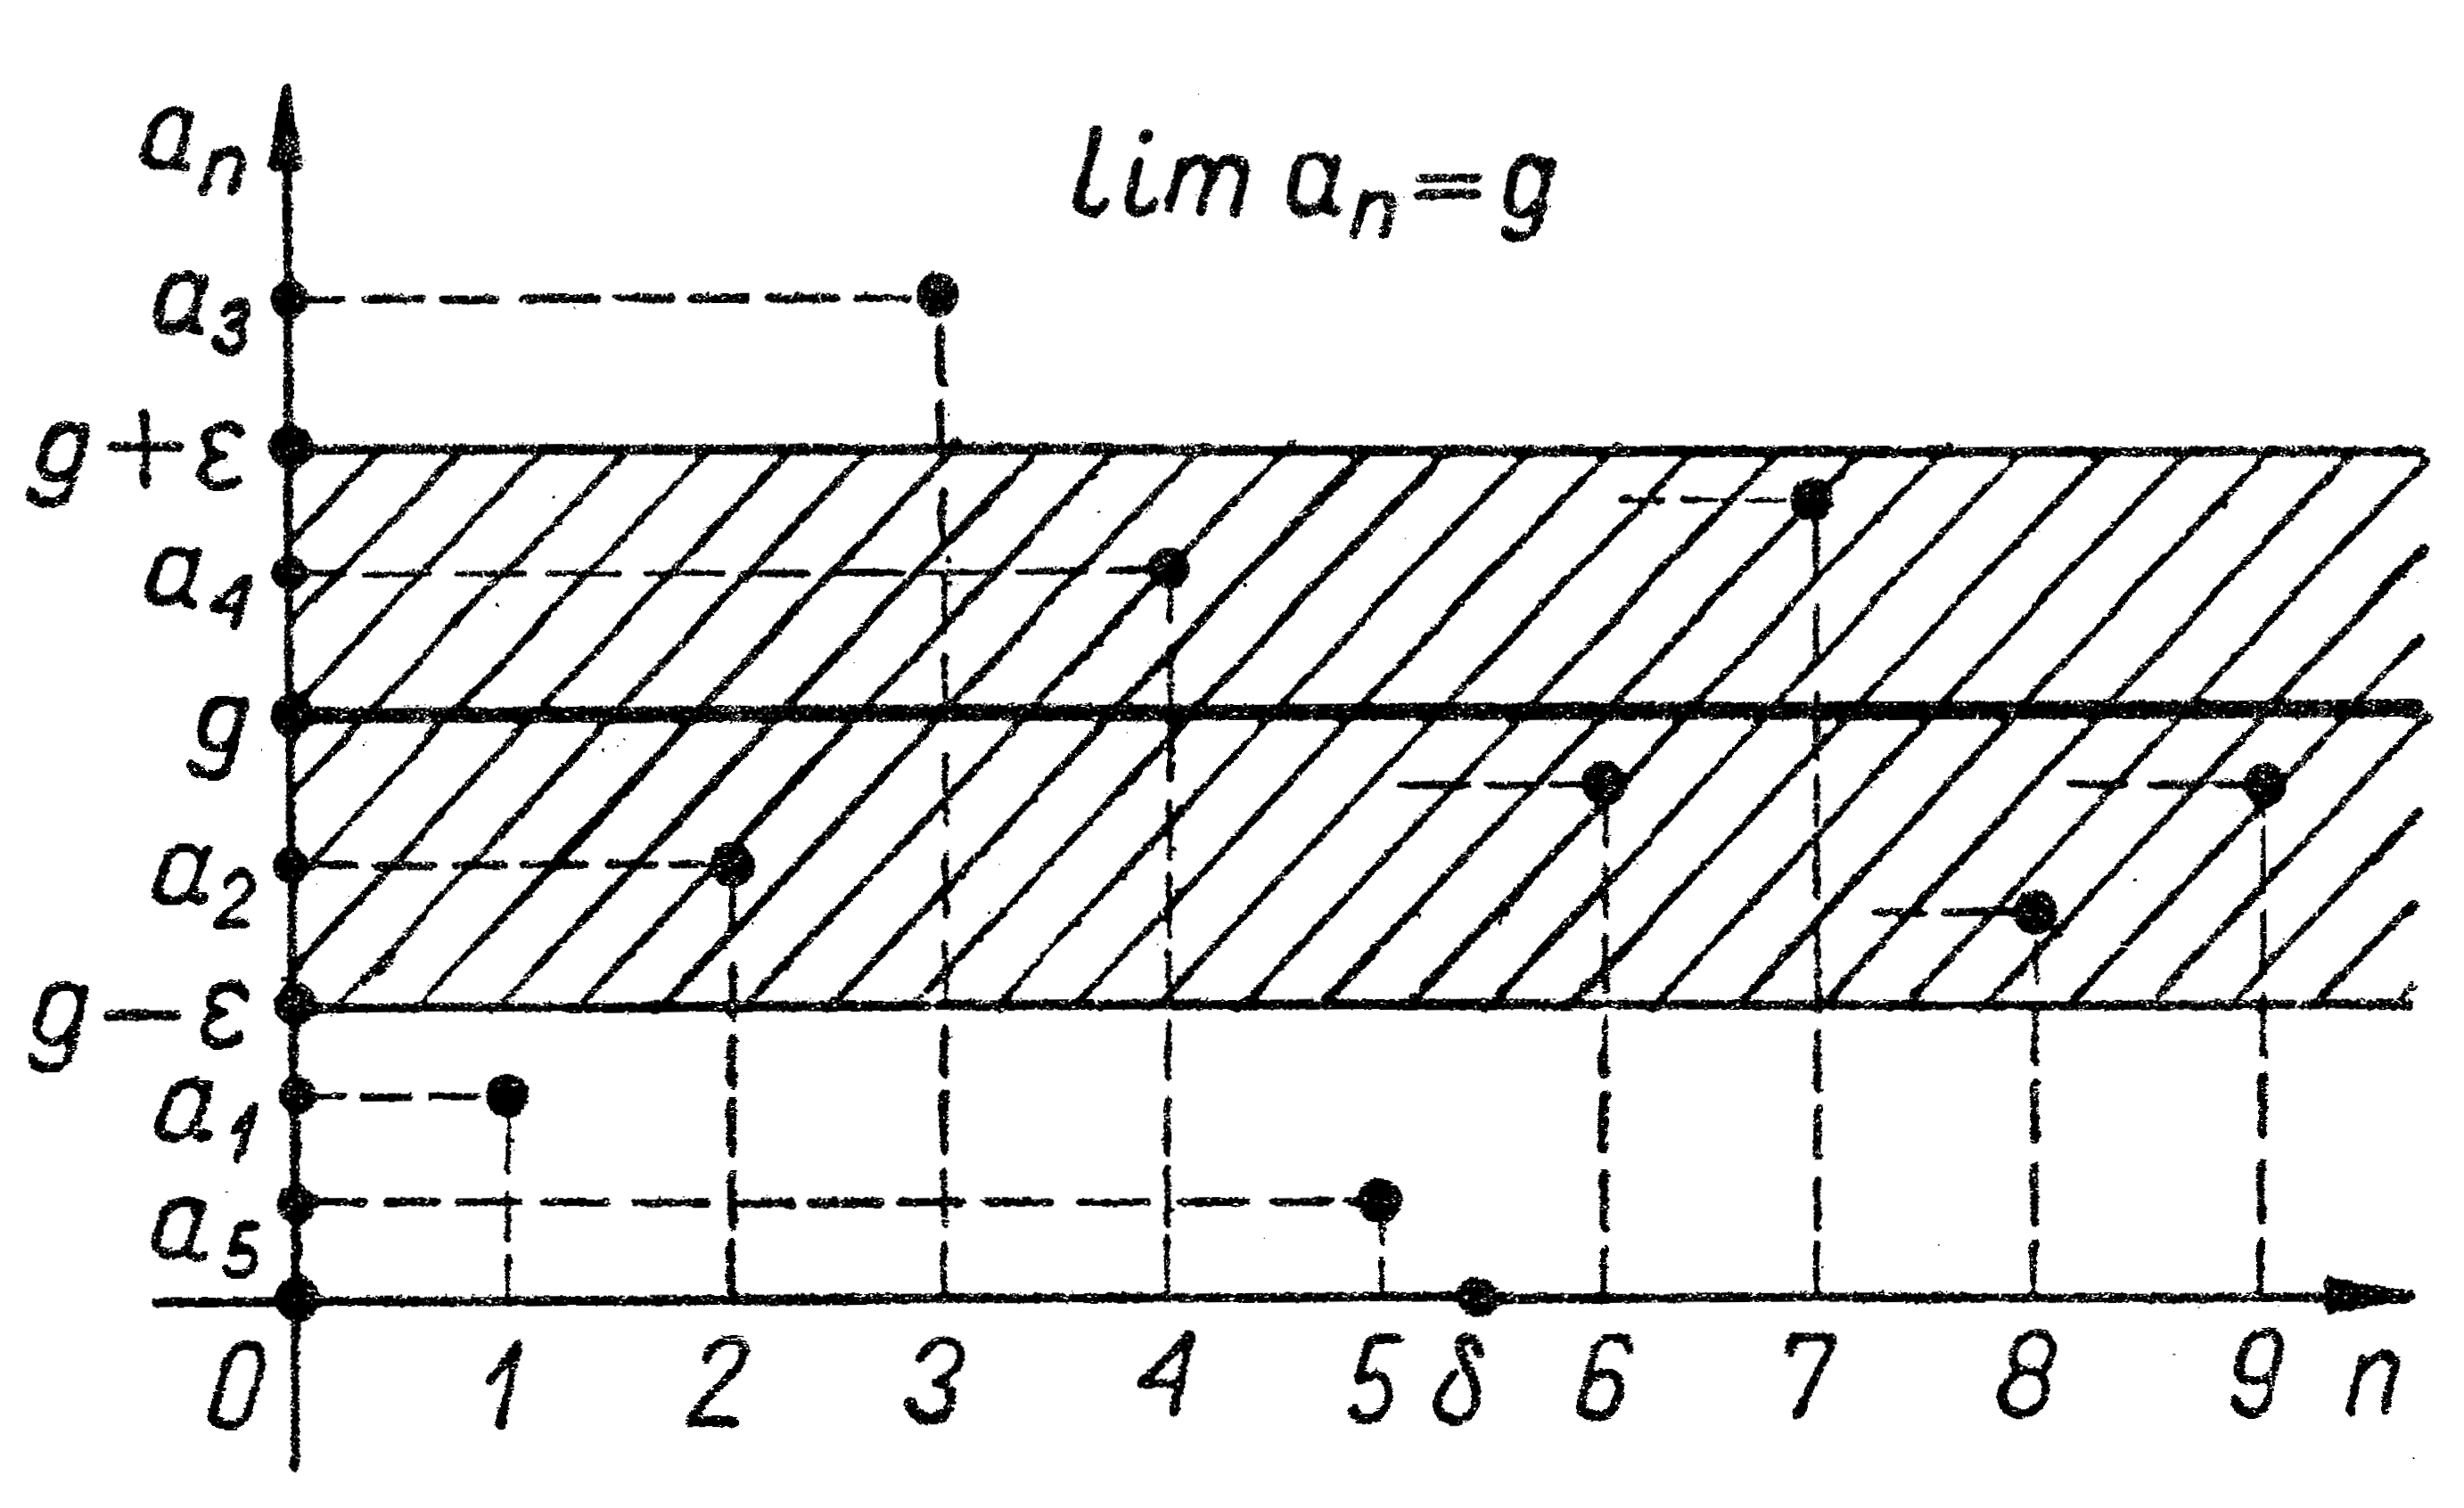
\includegraphics[scale=1.5]{img/ciagi-ciag_zbiezny.png}
\end{center}

\smallskip

\cite[Definicja 4.4]{ptak}
\end{definicja}

\bigskip

\begin{definicja}
M�wimy, �e ci�g $\left(a_n\right)$ jest \textbf{\emph{rozbie�ny do plus niesko�czono�ci}}\index{ci�g!rozbie�ny do plus niesko�czono�ci} wtedy i~tylko wtedy, gdy

\[
\forall \: M \quad \exists \: \delta \quad \forall \: n > \delta \qquad a_n > M
\]

\smallskip

\cite[Rozdzia� 2.1]{zakowski1}
\end{definicja}

\bigskip

\begin{definicja}
M�wimy, �e ci�g $\left(a_n\right)$ jest \textbf{\emph{rozbie�ny do minus niesko�czono�ci}}\index{ci�g!rozbie�ny do minus niesko�czono�ci} wtedy i~tylko wtedy, gdy

\[
\forall \: M \quad \exists \: \delta \quad \forall \: n > \delta \qquad a_n < M
\]

\smallskip

\cite[Rozdzia� 2.1]{zakowski1}
\end{definicja}

\bigskip
%%%%%%%%%%%%%%%%%%%%%%%%%%%%%%%
\section{Twierdzenia o ci�gach}

\begin{twierdzenie}[Zbie�no�� ci�g�w a dzia�ania]
Niech
\begin{itemize}
\item $\lim_{n \to \infty} a_n \; = \; a \: \in \: \mathbb{R}$,
\item $\lim_{n \to \infty} b_n \; = \; b \: \in \: \mathbb{R}$
\item oraz $\lambda \: \in \: \mathbb{R}$.
\end{itemize}

\medskip

\noindent Wtedy

\begin{itemize}
\item $\lim_{n \to \infty} \left(a_n \pm b_n \right) \; = \; a \pm b$
\item $\lim_{n \to \infty} \left(\lambda \: a_n\right) \; = \; \lambda \: a_n$
\item $\lim_{n \to \infty} \left(a_n \cdot b_n\right) \; = \; a_n \cdot b_n$
\item $\lim_{n \to \infty} \left(\dfrac{a_n}{b_n}\right) \; = \; \dfrac{a}{b}, \qquad b_n \neq 0, \quad b \neq 0$
\end{itemize}

\smallskip

\cite[Twierdzenie 4.14]{ptak}
\end{twierdzenie}

\bigskip

\begin{twierdzenie}
Je�li ci�g $\left(a_n\right)$ jest \textbf{zbie�ny} (Def. \ref{def:ciag_zbiezny}, str. \pageref{def:ciag_zbiezny}), to jest \textbf{ograniczony} (Def. \ref{def:ciag_ograniczony}, str. \pageref{def:ciag_ograniczony}).

\smallskip

\cite[Twierdzenie 4.18]{ptak}
\end{twierdzenie}

\bigskip

\begin{twierdzenie}[o trzech ci�gach]
Niech b�d� dane trzy ci�gi 

\[
\left(a_n\right), \left(b_n\right), \left(c_n\right)
\]

\noindent takie, �e

\[
a_n \leq b_n \leq c_n
\]

\noindent dla ka�dego $n > \delta \in \mathbb{N}$ oraz

\[
\lim_{n \to \infty} a_n \quad = \lim_{n \to \infty} c_n \quad = \quad g
\]

\noindent to $\left(b_n\right)$ jest \textbf{\emph{zbie�ny}}, a

\[
\lim_{n \to \infty} b_n \quad = \quad g
\]

\smallskip

\cite[Twierdzenie 4.21]{ptak}
\end{twierdzenie}

\bigskip

\begin{twierdzenie}
Ka�dy ci�g

\begin{itemize}
\item \textbf{rosn�cy} (Def. \ref{def:ciag_rosnacy}, str. \pageref{def:ciag_rosnacy})
\item i \textbf{ograniczony od g�ry} (Def. \ref{def:ciag_ograniczony_od_gory}, str. \pageref{def:ciag_ograniczony_od_gory})
\end{itemize}

\noindent jest \textbf{zbie�ny} (Def. \ref{def:ciag_zbiezny}, str. \pageref{def:ciag_zbiezny}).

\smallskip

\cite[Twierdzenie 4.23]{ptak}
\end{twierdzenie}

\bigskip

\begin{twierdzenie}
Ka�dy ci�g

\begin{itemize}
\item \textbf{malej�cy} (Def. \ref{def:ciag_malejacy}, str. \pageref{def:ciag_malejacy})
\item i \textbf{ograniczony od do�u} (Def. \ref{def:ciag_ograniczony_od_dolu}, str. \pageref{def:ciag_ograniczony_od_dolu})
\end{itemize}

\noindent jest \textbf{zbie�ny} (Def. \ref{def:ciag_zbiezny}, str. \pageref{def:ciag_zbiezny}).

\smallskip

\cite[Twierdzenie 4.23]{ptak}
\end{twierdzenie}

\chapter{Funkcje}

Definicj� funkcji Czytelnik znajdzie na stronie \pageref{def:funkcja}, a podstawowe definicje zwi�zane z ni� na stronie \pageref{podstawowe_definicje_dla_funkcji}.

\bigskip
%%%%%%%
\section{Wykres funkcji}

Funkcj� liczbow� mo�na interpretowa� geometrycznie sporz�dzaj�c tzw. \textbf{\emph{wykres funkcji}} (Def. \ref{def:wykres_funkcji}, str. \pageref{def:wykres_funkcji}).

Na p�aszczy�nie kartezja�skiego uk�adu wsp�rz�dnych zaznaczamy punkty o wsp�rz�dnych $\left(x, f(x)\right)$, kt�rych zbi�r, gdy $x$ przyjmuje wszystkie warto�ci dziedziny funkcji (Def. \ref{def:dziedzina_funkcji}, str. \pageref{def:dziedzina_funkcji}) $f$, stanowi wykres funkcji.

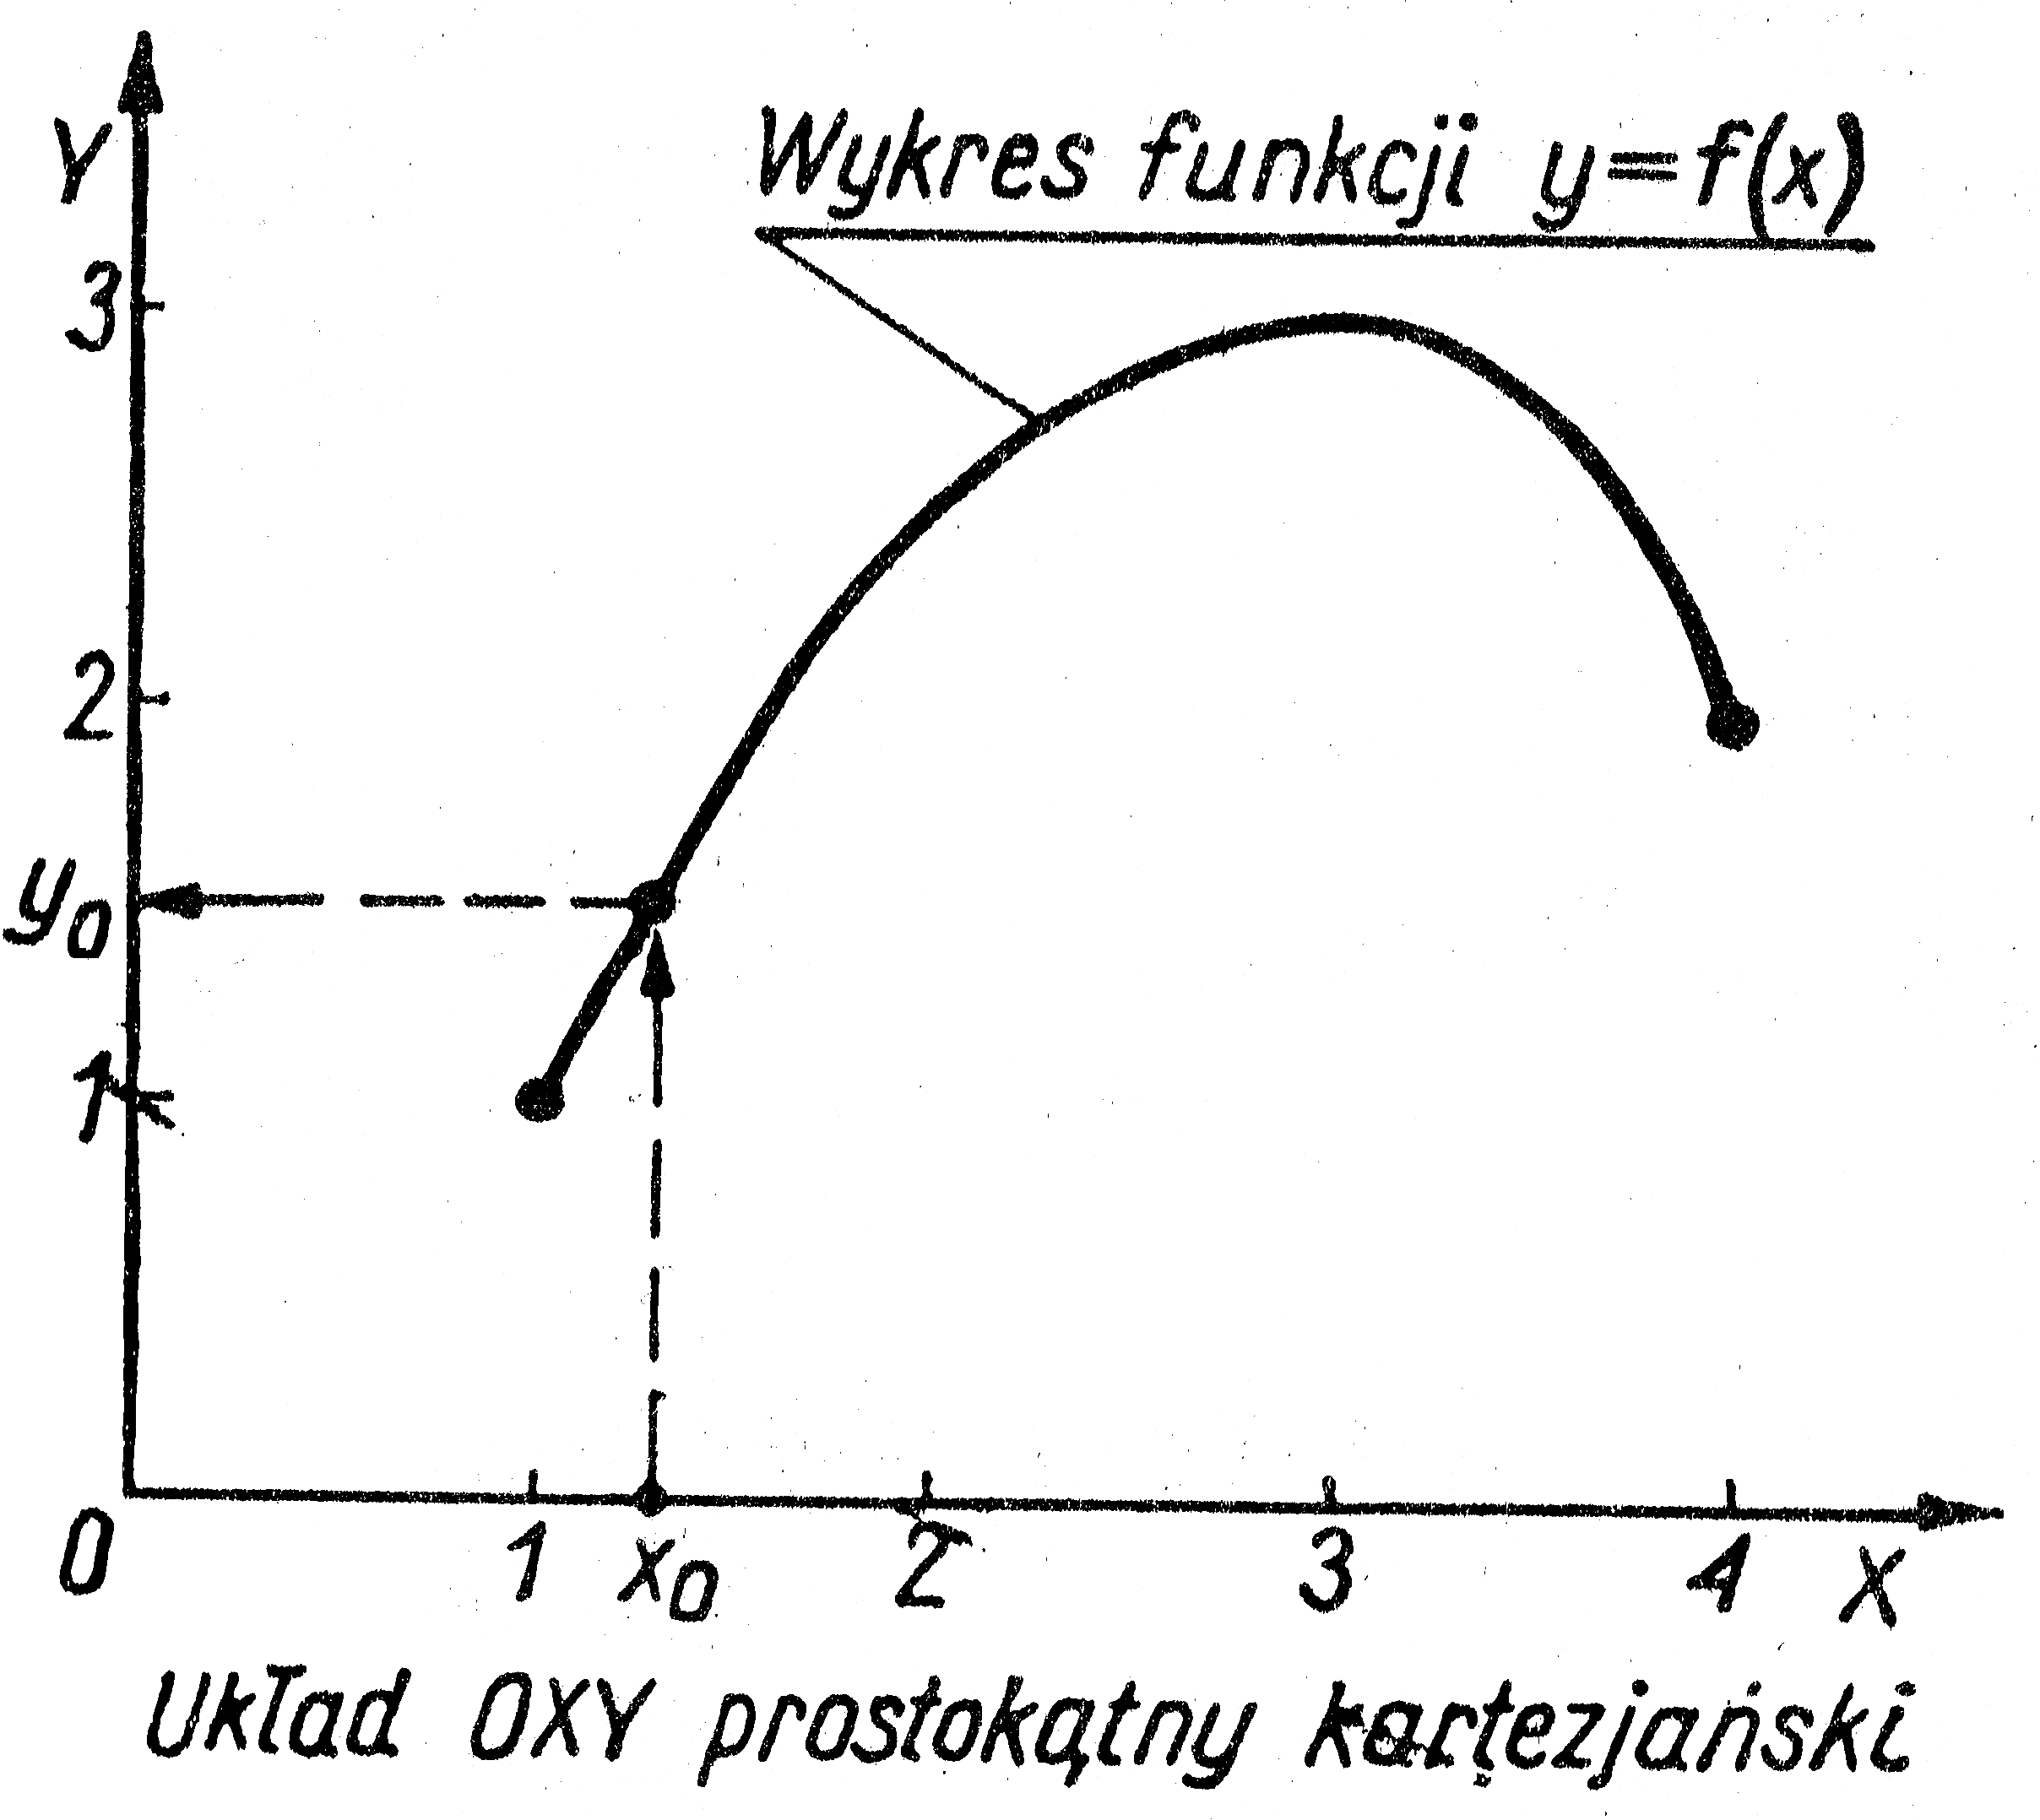
\includegraphics[scale=1.5]{img/funkcje-wykres_funkcji.png}

\cite[Rozdzia� 1.7]{zakowski1}

\bigskip
%%%%%%%
\section{Wykres funkcji odwrotnej}

Niech
\[
y = f(x)
\]
oraz
\[
y = f^{-1}(x)
\]
(Def. \ref{def:relacja_odwrotna}, str. \pageref{def:relacja_odwrotna})

\medskip

Wykres funkcji $f$ i wykres funkcji odwrotnej $f^{-1}$ s� symetrycznie po�o�one wzgl�dem dwusiecznej k�ta zawartego mi�dzy dodatnimi p�osiami wsp�rz�dnych

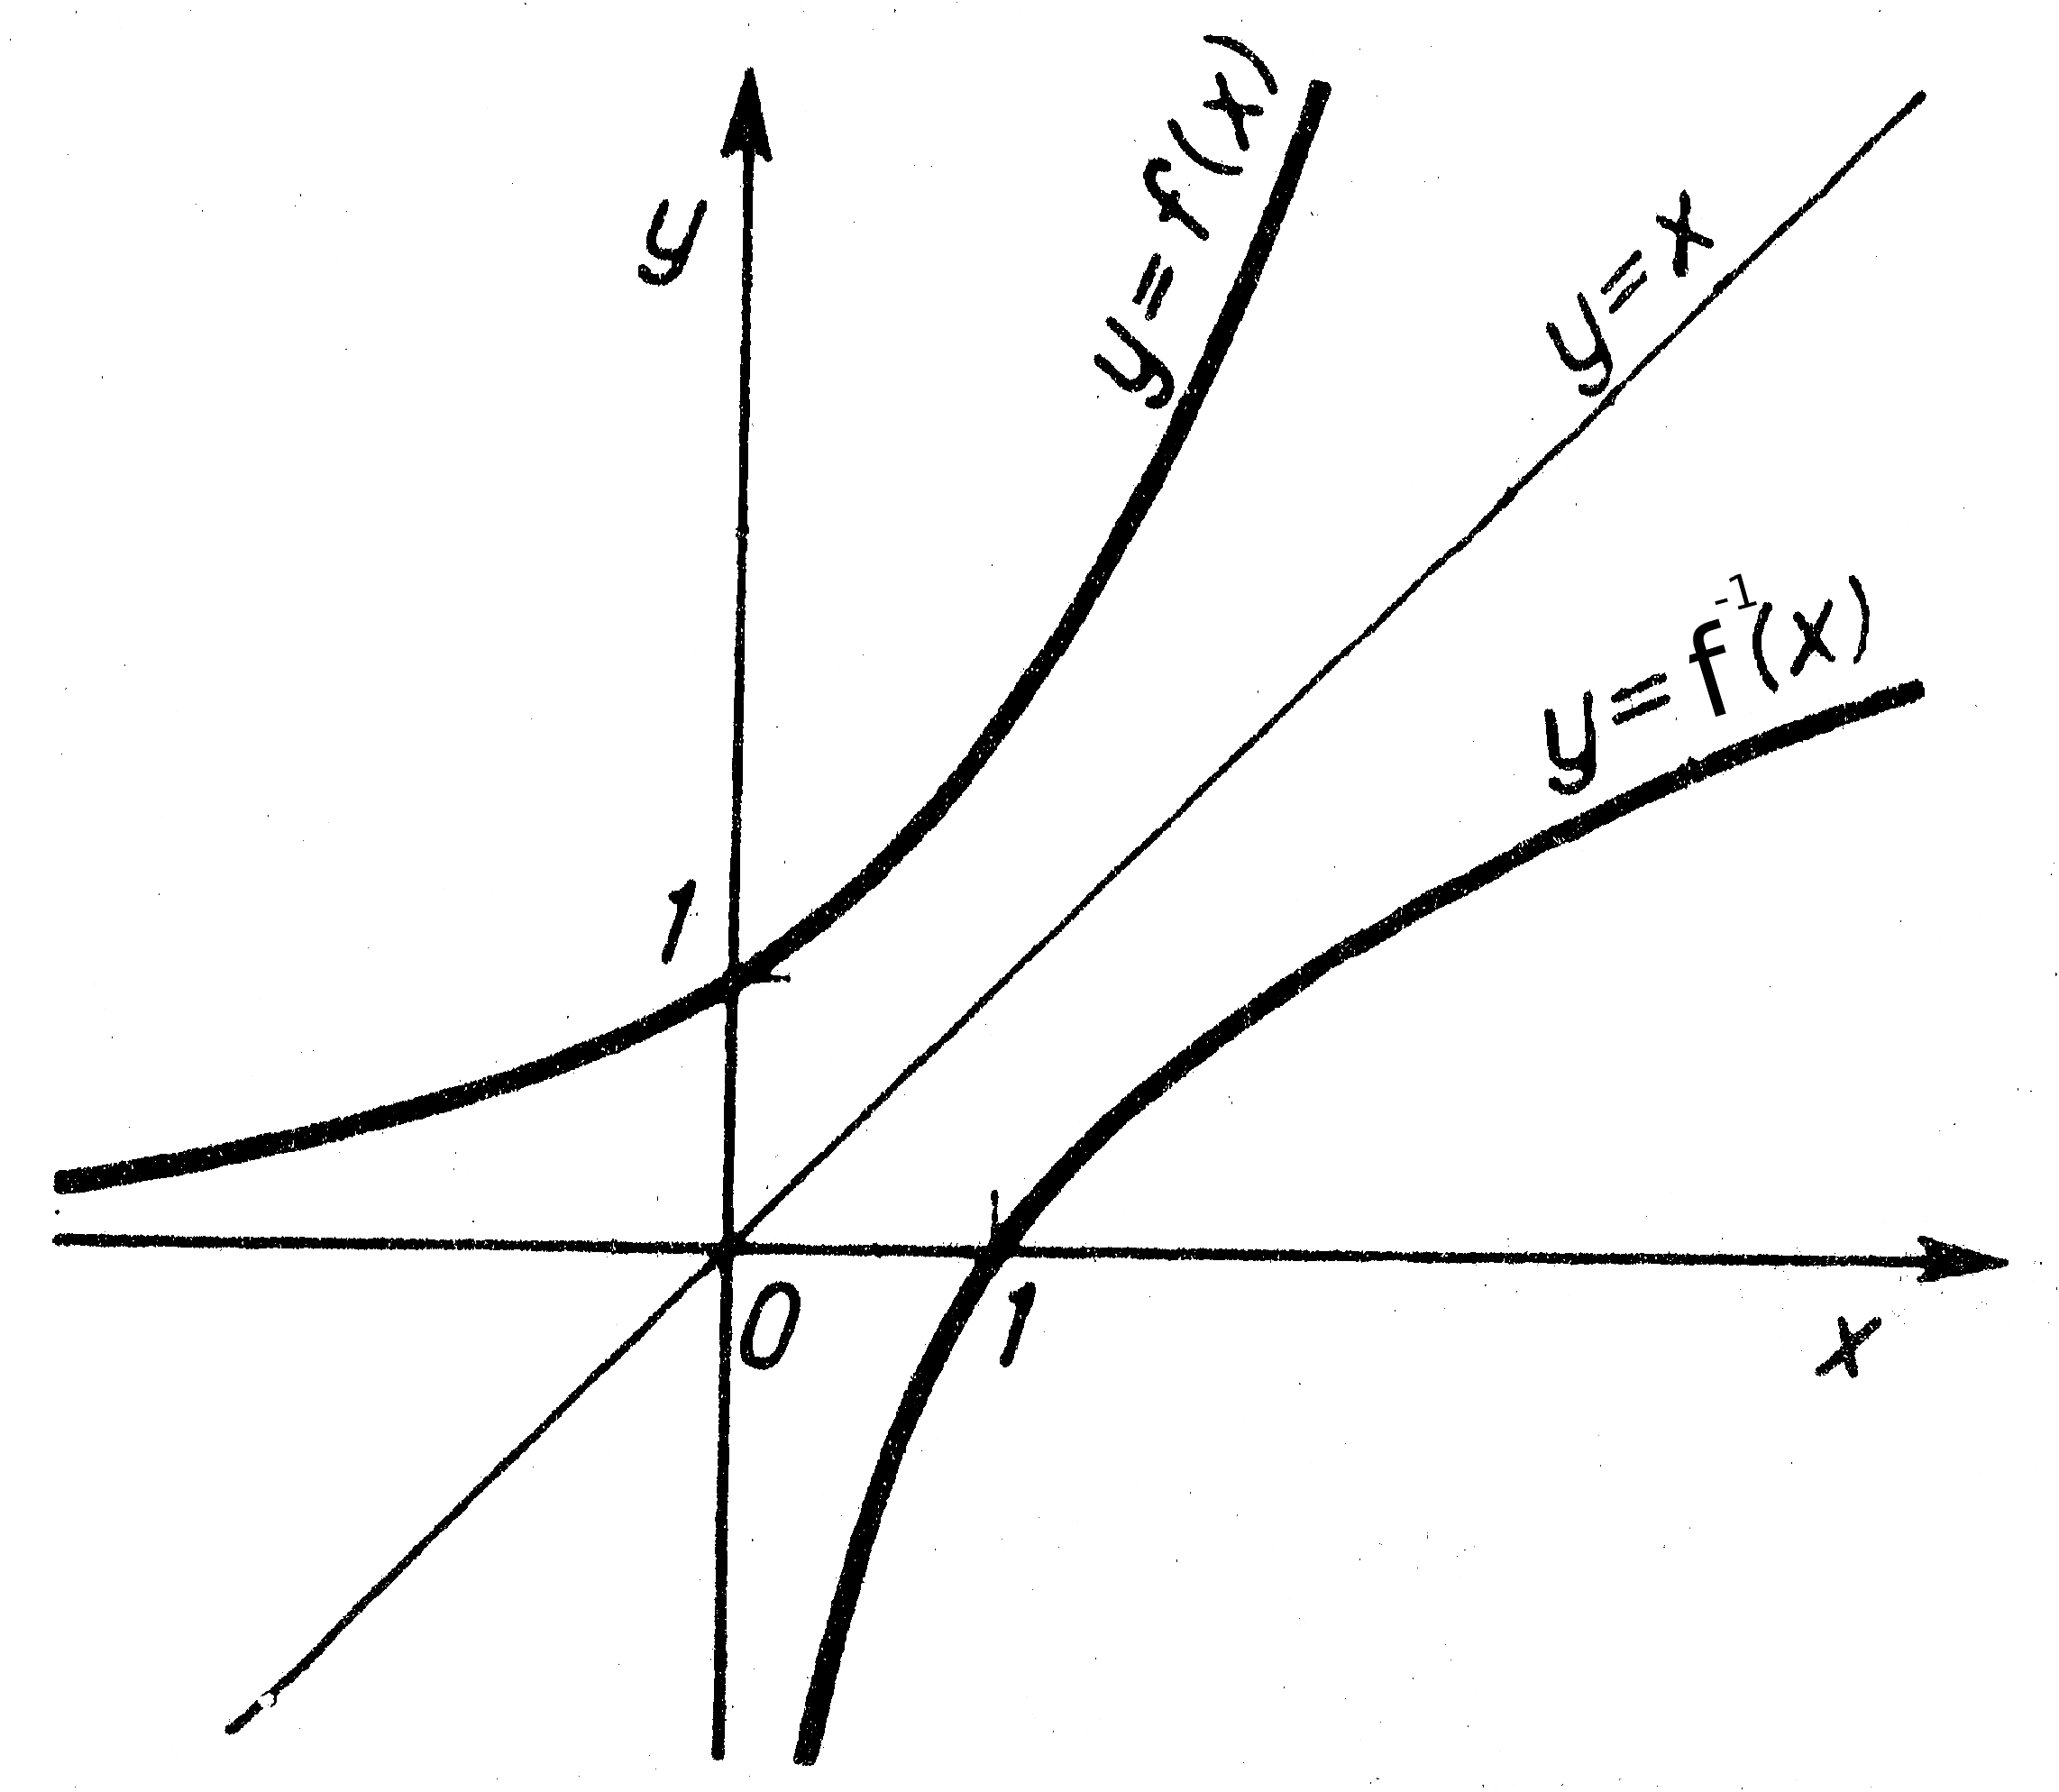
\includegraphics[scale=1.5]{img/funkcje-funkcja_odwrotna.png}

\cite[Paragraf 4.7]{krysicki1}

\bigskip
%%%%%%%
\section{Parzysto��. Nieparzysto��}

TODO Df

\begin{definicja}
Funkcj� $f \colon \mathbb{R} \supset Df \rightarrow \mathbb{R}$ nazywamy \textbf{\emph{parzyst�}}\label{def:funkcja_parzysta}, je�li
\[
\forall x \in Df \colon \qquad -x \in Df \quad \wedge \quad f(-x) = f(x)
\]
\end{definicja}

\medskip

\begin{definicja}
Funkcj� $f \colon \mathbb{R} \supset Df \rightarrow \mathbb{R}$ nazywamy \textbf{\emph{nieparzyst�}}\label{def:funkcja_nieparzysta}, je�li
\[
\forall x \in Df \colon \qquad -x \in Df \quad \wedge \quad f(-x) = -f(x)
\]
\end{definicja}

\cite[Rozdzia� 5.2]{ptak}


\bigskip
%%%%%%%%%%%%%%%%%%%%%%%%%
\section{Granice funkcji}

%%%%%%%%%%%%%%%%%%%%%%%%%%%%%%%%%%%%%
\subsection{Granica lewostronna funkcji}

\begin{definicja}[Cauchy'ego]
M�wimy, �e liczba $g$ jest \textbf{\emph{granic� lewostronn� funkcji}}\label{def:granica_lewostronna_funkcji} $f(x)$ w punkcie $x = x_0$, co zapisujemy

\[
\lim_{x \to x_0^-} f(x) \; = \; g
\]

je�eli dla ka�dego $\varepsilon > 0$ istnieje taka liczba $\delta > 0$, �e

\[
\left| f(x) - g \right| < \varepsilon \qquad \textsl{ dla } \qquad x_0 - \delta < x < x_0
\]

\medskip

Lub symbolicznie

\[
\lim_{x \to x_0^-} f(x) \: = \: g 
\]
\[
\Updownarrow
\]
\[
\forall \varepsilon\!>\!0 \quad \exists \delta\!>\!0 \quad \forall x \colon \qquad x_0 - \delta < x < x_0 \quad \Rightarrow \quad \left| f(x) - g \right| < \varepsilon
\]


\cite[Paragraf 5.1]{krysicki1}
\end{definicja}

\bigskip

\begin{definicja}[Heinego]
M�wimy, �e fukcja $f(x)$ ma w punkcie $x_0$ \textbf{\emph{granic� lewostronn�}} i piszemy

\[
\lim_{x \to x_0^-} f(x) \: = \: g 
\]
\[
\Updownarrow
\]
\[
\forall (x_n) \subset \{x_n \subset Df, x_n < x_0\} \colon \qquad \lim_{n \to \infty} x_n = x_0 \quad \Rightarrow \quad \lim_{n \to \infty} f\left(x_n\right) = g
\]

\cite[Rozdzia� 2.3]{zakowski1} \cite[Twierdzenie 5.33]{ptak} \cite[Paragraf 5.1]{krysicki1}
\end{definicja}

\bigskip
%%%%%%%%%%%%%%%%%%%%%%%%%%%%%%%%%%%%%%
\subsection{Granica prawostronna funkcji}

\begin{definicja}[Cauchy'ego]
M�wimy, �e liczba $g$ jest \textbf{\emph{granic� prawostronn� funkcji}}\label{def:granica_prawostronna_funkcji} $f(x)$ w punkcie $x = x_0$, co zapisujemy

\[
\lim_{x \to x_0^+} f(x) \; = \; g
\]

je�eli dla ka�dego $\varepsilon > 0$ istnieje taka liczba $\delta > 0$, �e

\[
\left| f(x) - g \right| < \varepsilon \qquad \textsl{ dla } \qquad x_0 < x < x_0 + \delta
\]

\medskip

Lub symbolicznie

\[
\lim_{x \to x_0^+} f(x) \: = \: g 
\]
\[
\Updownarrow
\]
\[
\forall \varepsilon\!>\!0 \quad \exists \delta\!>\!0 \quad \forall x \colon \qquad x_0 < x < x_0 + \delta \quad \Rightarrow \quad \left| f(x) - g \right| < \varepsilon
\]


\cite[Paragraf 5.1]{krysicki1}
\end{definicja}

\bigskip

\begin{definicja}[Heinego] TODO Df
M�wimy, �e fukcja $f(x)$ ma w punkcie $x_0$ \textbf{\emph{granic� prawostronn�}} i piszemy

\[
\lim_{x \to x_0^+} f(x) \: = \: g 
\]
\[
\Updownarrow
\]
\[
\forall (x_n) \subset \{x_n \subset Df, x_n > x_0\} \colon \qquad \lim_{n \to \infty} x_n = x_0 \quad \Rightarrow \quad \lim_{n \to \infty} f\left(x_n\right) = g
\]

\cite[Rozdzia� 2.3]{zakowski1} \cite[Twierdzenie 5.33]{ptak} \cite[Paragraf 5.1]{krysicki1}
\end{definicja}

\bigskip
%%%%%%%%%%%%%%%%%%%%%%%%%
\subsection{Granica funkcji}

\begin{definicja}[Cauchy'ego]
M�wimy, �e liczba $g$ jest \textbf{\emph{granic� funkcji}}\label{def:granica_funkcji} $f(x)$ w punkcie $x = x_0$, co zapisujemy

\[
\lim_{x \to x_0} f(x) \; = \; g
\]

je�eli dla ka�dego $\varepsilon > 0$ istnieje taka liczba $\delta > 0$, �e

\[
\left| f(x) - g \right| < \varepsilon \qquad \textsl{ dla } \qquad \left|x - x_0\right| < \delta
\]

\medskip

Lub symbolicznie

\[
\lim_{x \to x_0} f(x) \: = \: g 
\]
\[
\Updownarrow
\]
\[
\forall \varepsilon\!>\!0 \quad \exists \delta\!>\!0 \quad \forall x \colon \qquad \left|x - x_0\right| < \delta \quad \Rightarrow \quad \left| f(x) - g \right| < \varepsilon
\]


\cite[Paragraf 5.1]{krysicki1}
\end{definicja}

\bigskip

\begin{definicja}[Heinego] TODO (Df)
M�wimy, �e fukcja $f(x)$ ma w punkcie $x_0$ \textbf{\emph{granic�}} i piszemy

\[
\lim_{x \to x_0} f(x) \: = \: g 
\]
\[
\Updownarrow
\]
\[
\forall (x_n) \subset Df\setminus \{x_0\} \colon \qquad \lim_{n \to \infty} x_n = x_0 \quad \Rightarrow \quad \lim_{n \to \infty} f\left(x_n\right) = g
\]

\cite[Rozdzia� 2.3]{zakowski1} \cite[Twierdzenie 5.33]{ptak} \cite[Paragraf 5.1]{krysicki1}
\end{definicja}


\bigskip
%%%%%%%%%%%%%%%%%%%%%%%%%%%%%%%%%%%%%%%%%%%%%%
\subsection{Interpretacja geometryczna granic}

Zapis
\[
\lim_{x \to x_0^-}
\]

\noindent geometrycznie oznacza, �e jakikolwiek we�miemy w�ski pasek

\begin{equation}
\label{igg:pasek_l} g - \varepsilon \; < \; y \; < \; g + \varepsilon
\end{equation}

\noindent to musi istnie� takie \emph{otoczenie lewostronne} punktu $x = x_0$, czyli taki przedzia�

\begin{equation}
\label{igg:otoczenie_l} x_0 - h \;< \;x \;< \;x_0, \qquad \textsl{ gdzie } \quad h > 0
\end{equation}

\noindent �e ca�y wykres funkcji dla $x$ z przedzia�u (\ref{igg:otoczenie_l}) znajduje si� w pasku (\ref{igg:pasek_l}).

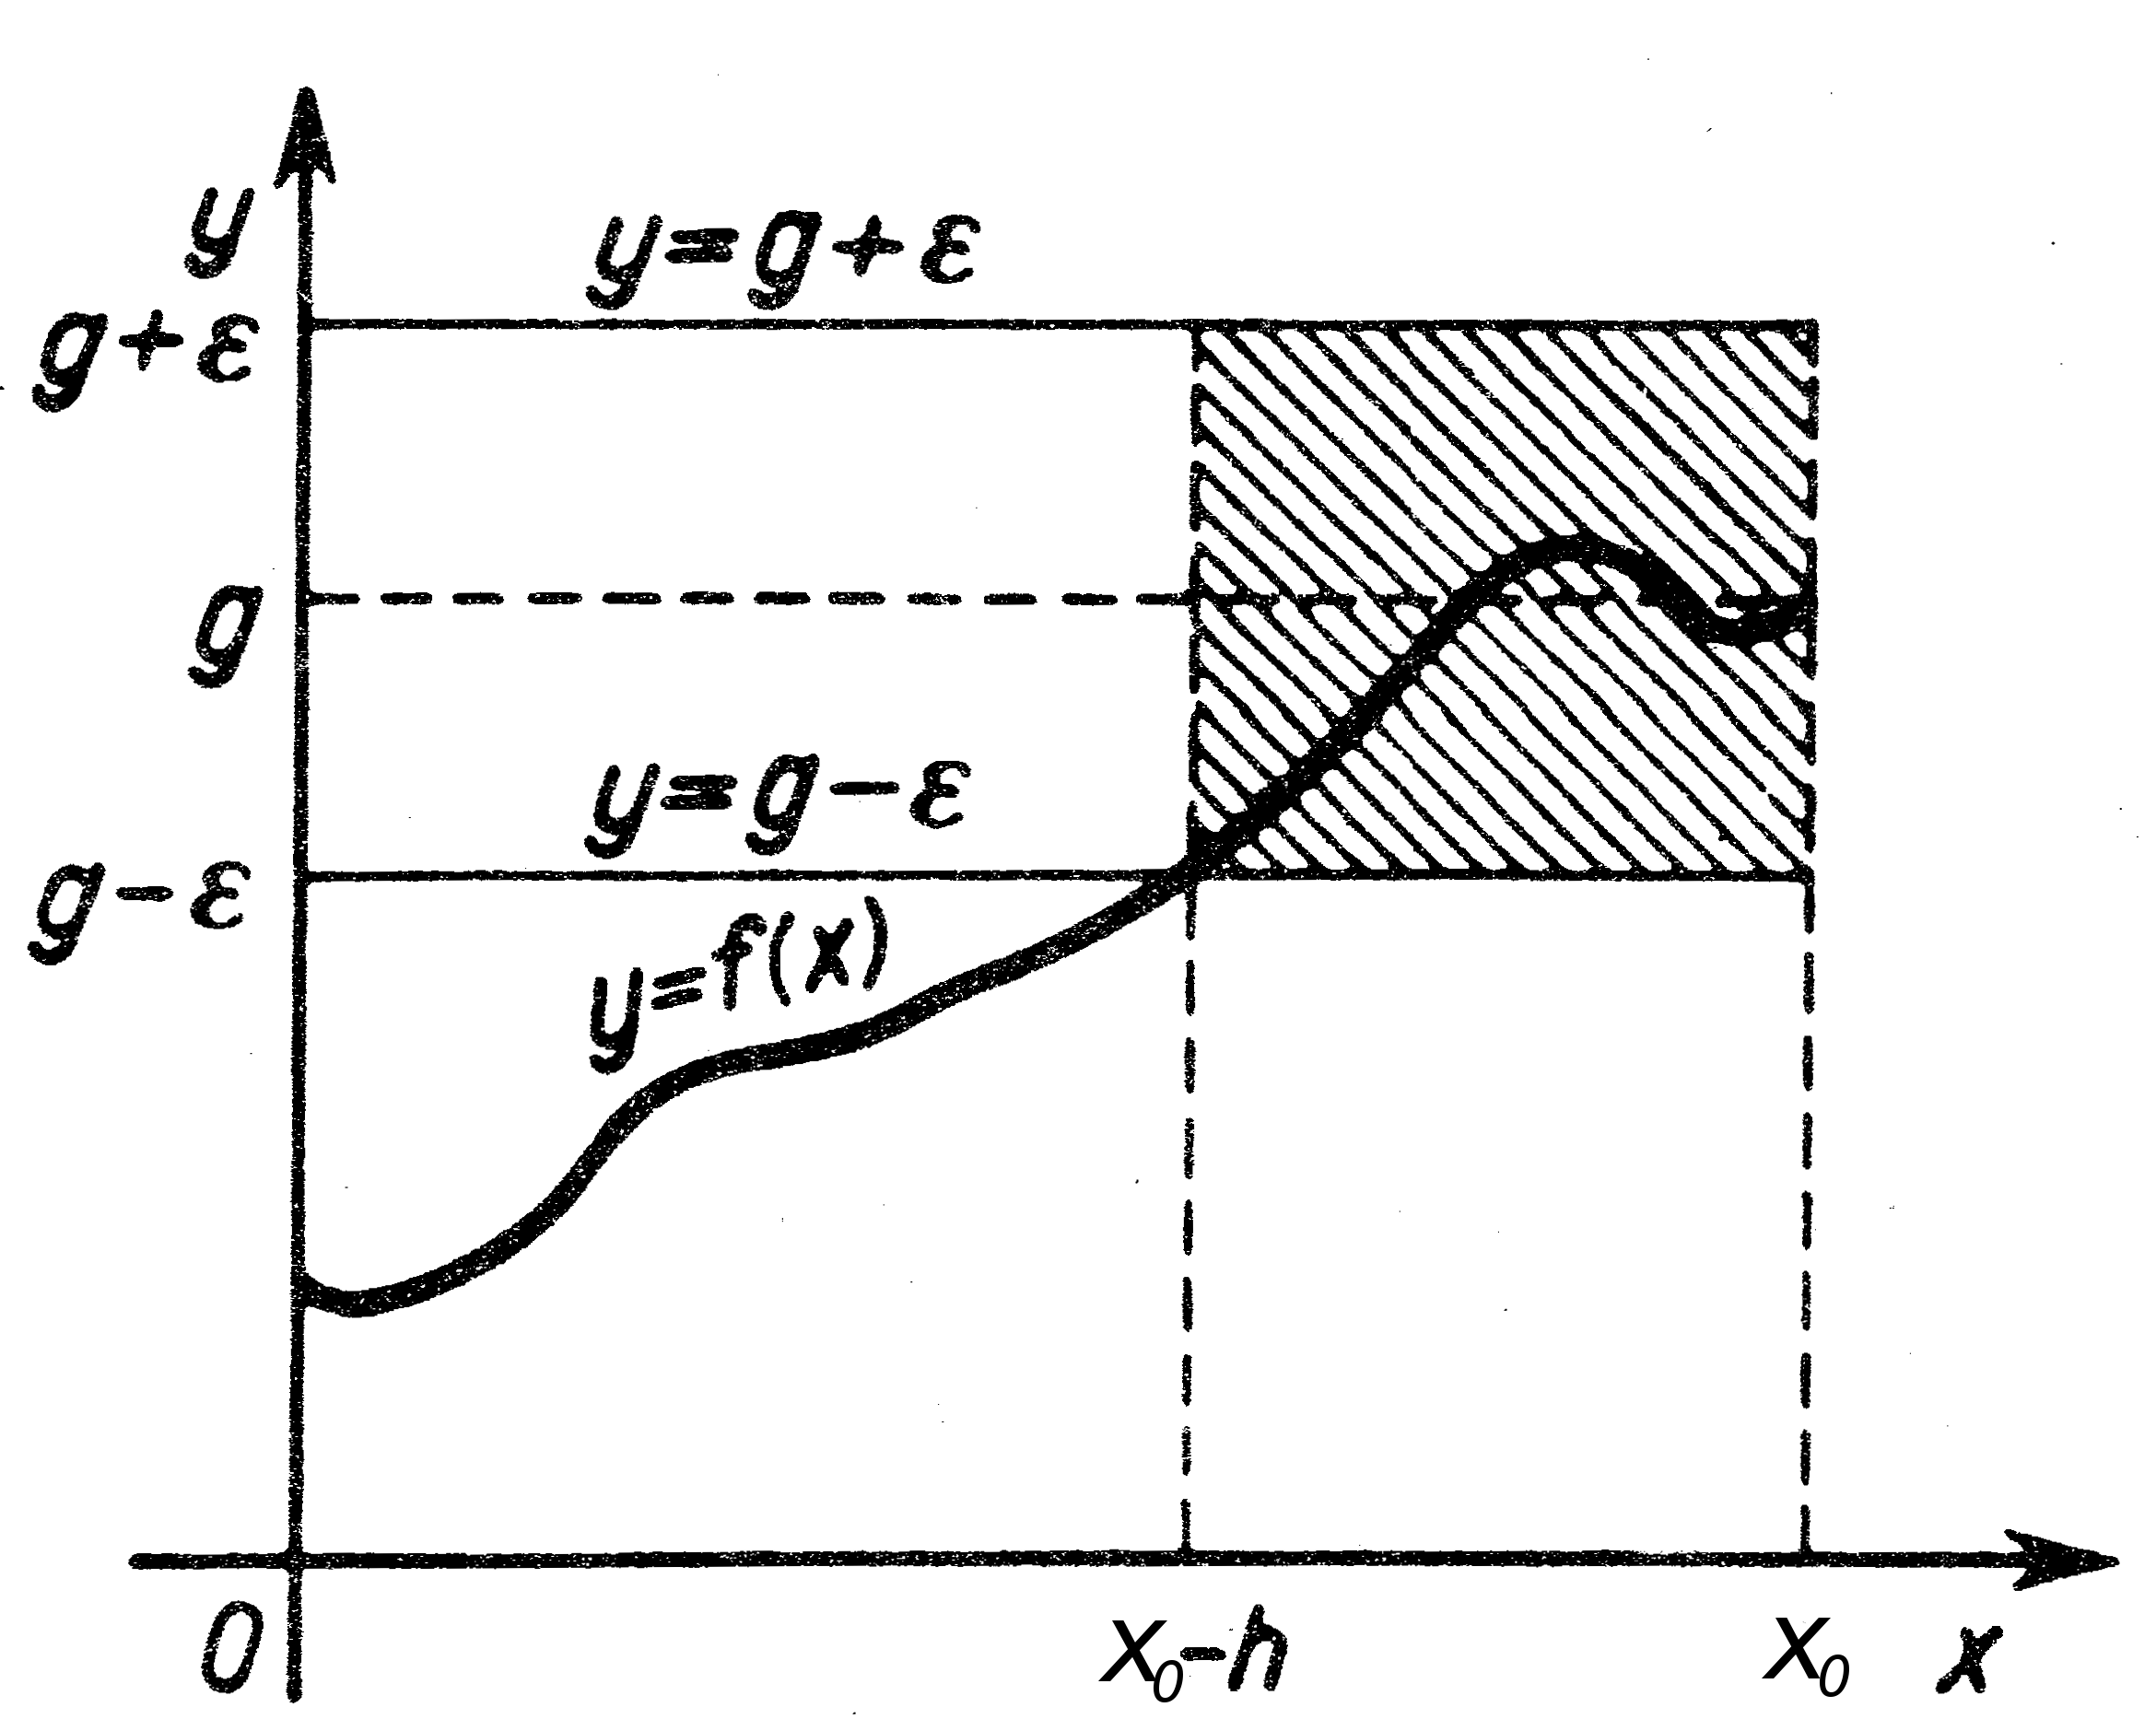
\includegraphics[scale=1.5]{img/funkcje-interpretacja_granicy-l.png}

\bigskip

Zapis
\[
\lim_{x \to x_0^+}
\]

\noindent geometrycznie oznacza, �e jakikolwiek we�miemy w�ski pasek

\begin{equation}
\label{igg:pasek_p} g - \varepsilon \; < \; y \; < \; g + \varepsilon
\end{equation}

\noindent to musi istnie� takie \emph{otoczenie prawostronne} punktu $x = x_0$, czyli taki przedzia�

\begin{equation}
\label{igg:otoczenie_p} x_0 \;< \;x \;< \;x_0 + h, \qquad \textsl{ gdzie } \quad h > 0
\end{equation}

\noindent �e ca�y wykres funkcji dla $x$ z przedzia�u (\ref{igg:otoczenie_p}) znajduje si� w pasku (\ref{igg:pasek_p}).

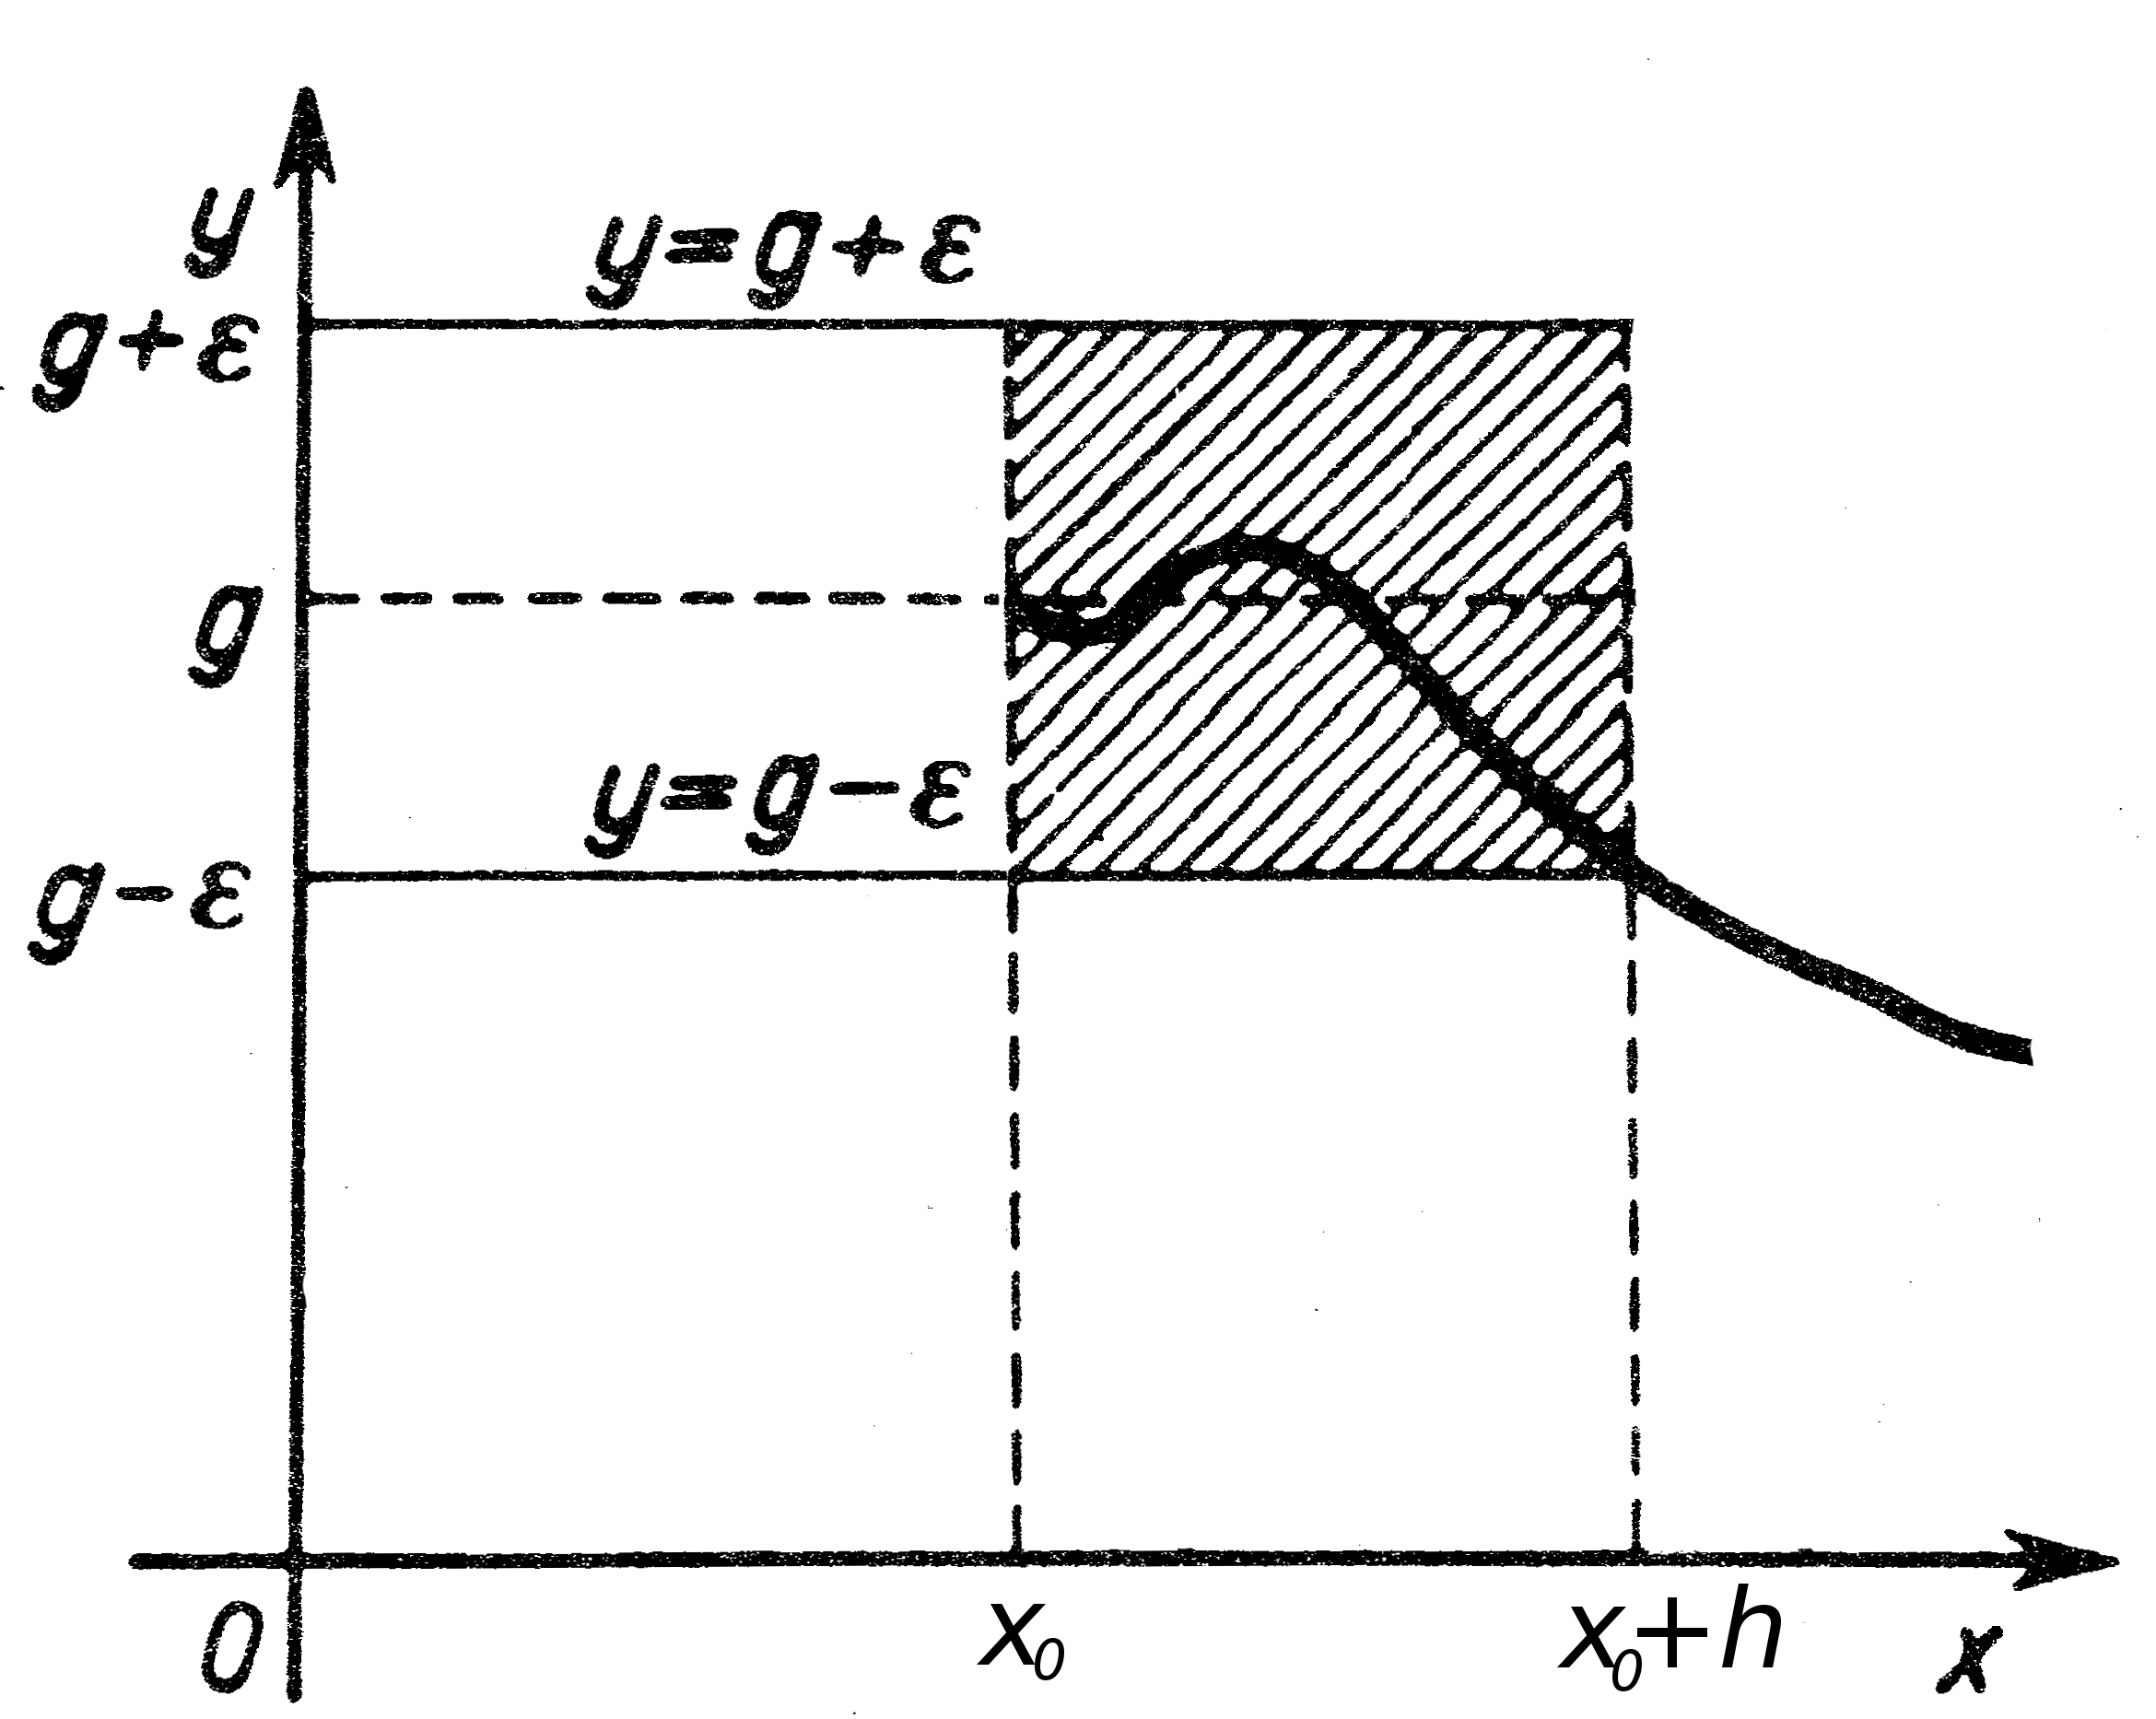
\includegraphics[scale=1.5]{img/funkcje-interpretacja_granicy-p.png}

\cite[Paragraf 5.2]{krysicki1}

\bigskip
%%%%%%%%%%%%%%%%%%%%%%%%%%%%%%%%%%%%
\subsection{Twierdzenia o granicach}

\begin{twierdzenie}[granice a dzia�ania]
Niech $\lim_{x \to x_0} f(x) = a$, $\lim_{x \to x_0} g(x) = b$ oraz $a, \:b, \:\lambda \: \in \mathbb{R}$. Wtedy

\begin{itemize}
\item $\lim_{x \to x_O} \left(f(x) \pm g(x)\right) \; = \; a \pm b$
\item $\lim_{x \to x_O} \lambda f(x) \; = \; \lambda a$
\item $\lim_{x \to x_O} \left(f(x) \cdot g(x)\right) \; = \; ab$
\item $\lim_{x \to x_O} \dfrac{(f(x)}{g(x)} \; = \; \dfrac{a}{b}$, je�li $b \neq 0$
\end{itemize}

\cite[Twierdzenie 5.37]{ptak}
\end{twierdzenie}

\bigskip

\begin{twierdzenie}[l'H\^{o}spitala]
TODO
\end{twierdzenie}

\bigskip
%%%%%%%%%%%%%%%%%%
\section{Ci�g�o��}

%%%%%%%%%%%%%%%%%%%%%%%%%%%%%%%%%
\subsection{Definicja Cauchy'ego}

\begin{definicja}[Cauchy'ego]
M�wimy, �e funkcja $f$ jest \textbf{\emph{ci�g�a w punkcie $x_0$}}\label{def:funkcja_ciagla_w_punkcie} wtedy i~tylko wtedy, gdy (TODO Df)

\begin{tabular*}{\textwidth}%
{@{\extracolsep{\stretch{1}}}lc}
& \\
$\forall \varepsilon > 0 \quad \exists \delta > 0 \quad \forall x \in Df$
& \vspace{0.3cm} \\
\multicolumn{2}{c}{
$|x - x_0| < \delta \quad \Rightarrow \quad |f(x) - f(x_0)| < \varepsilon$
\vspace{0.3cm}
}
\end{tabular*}

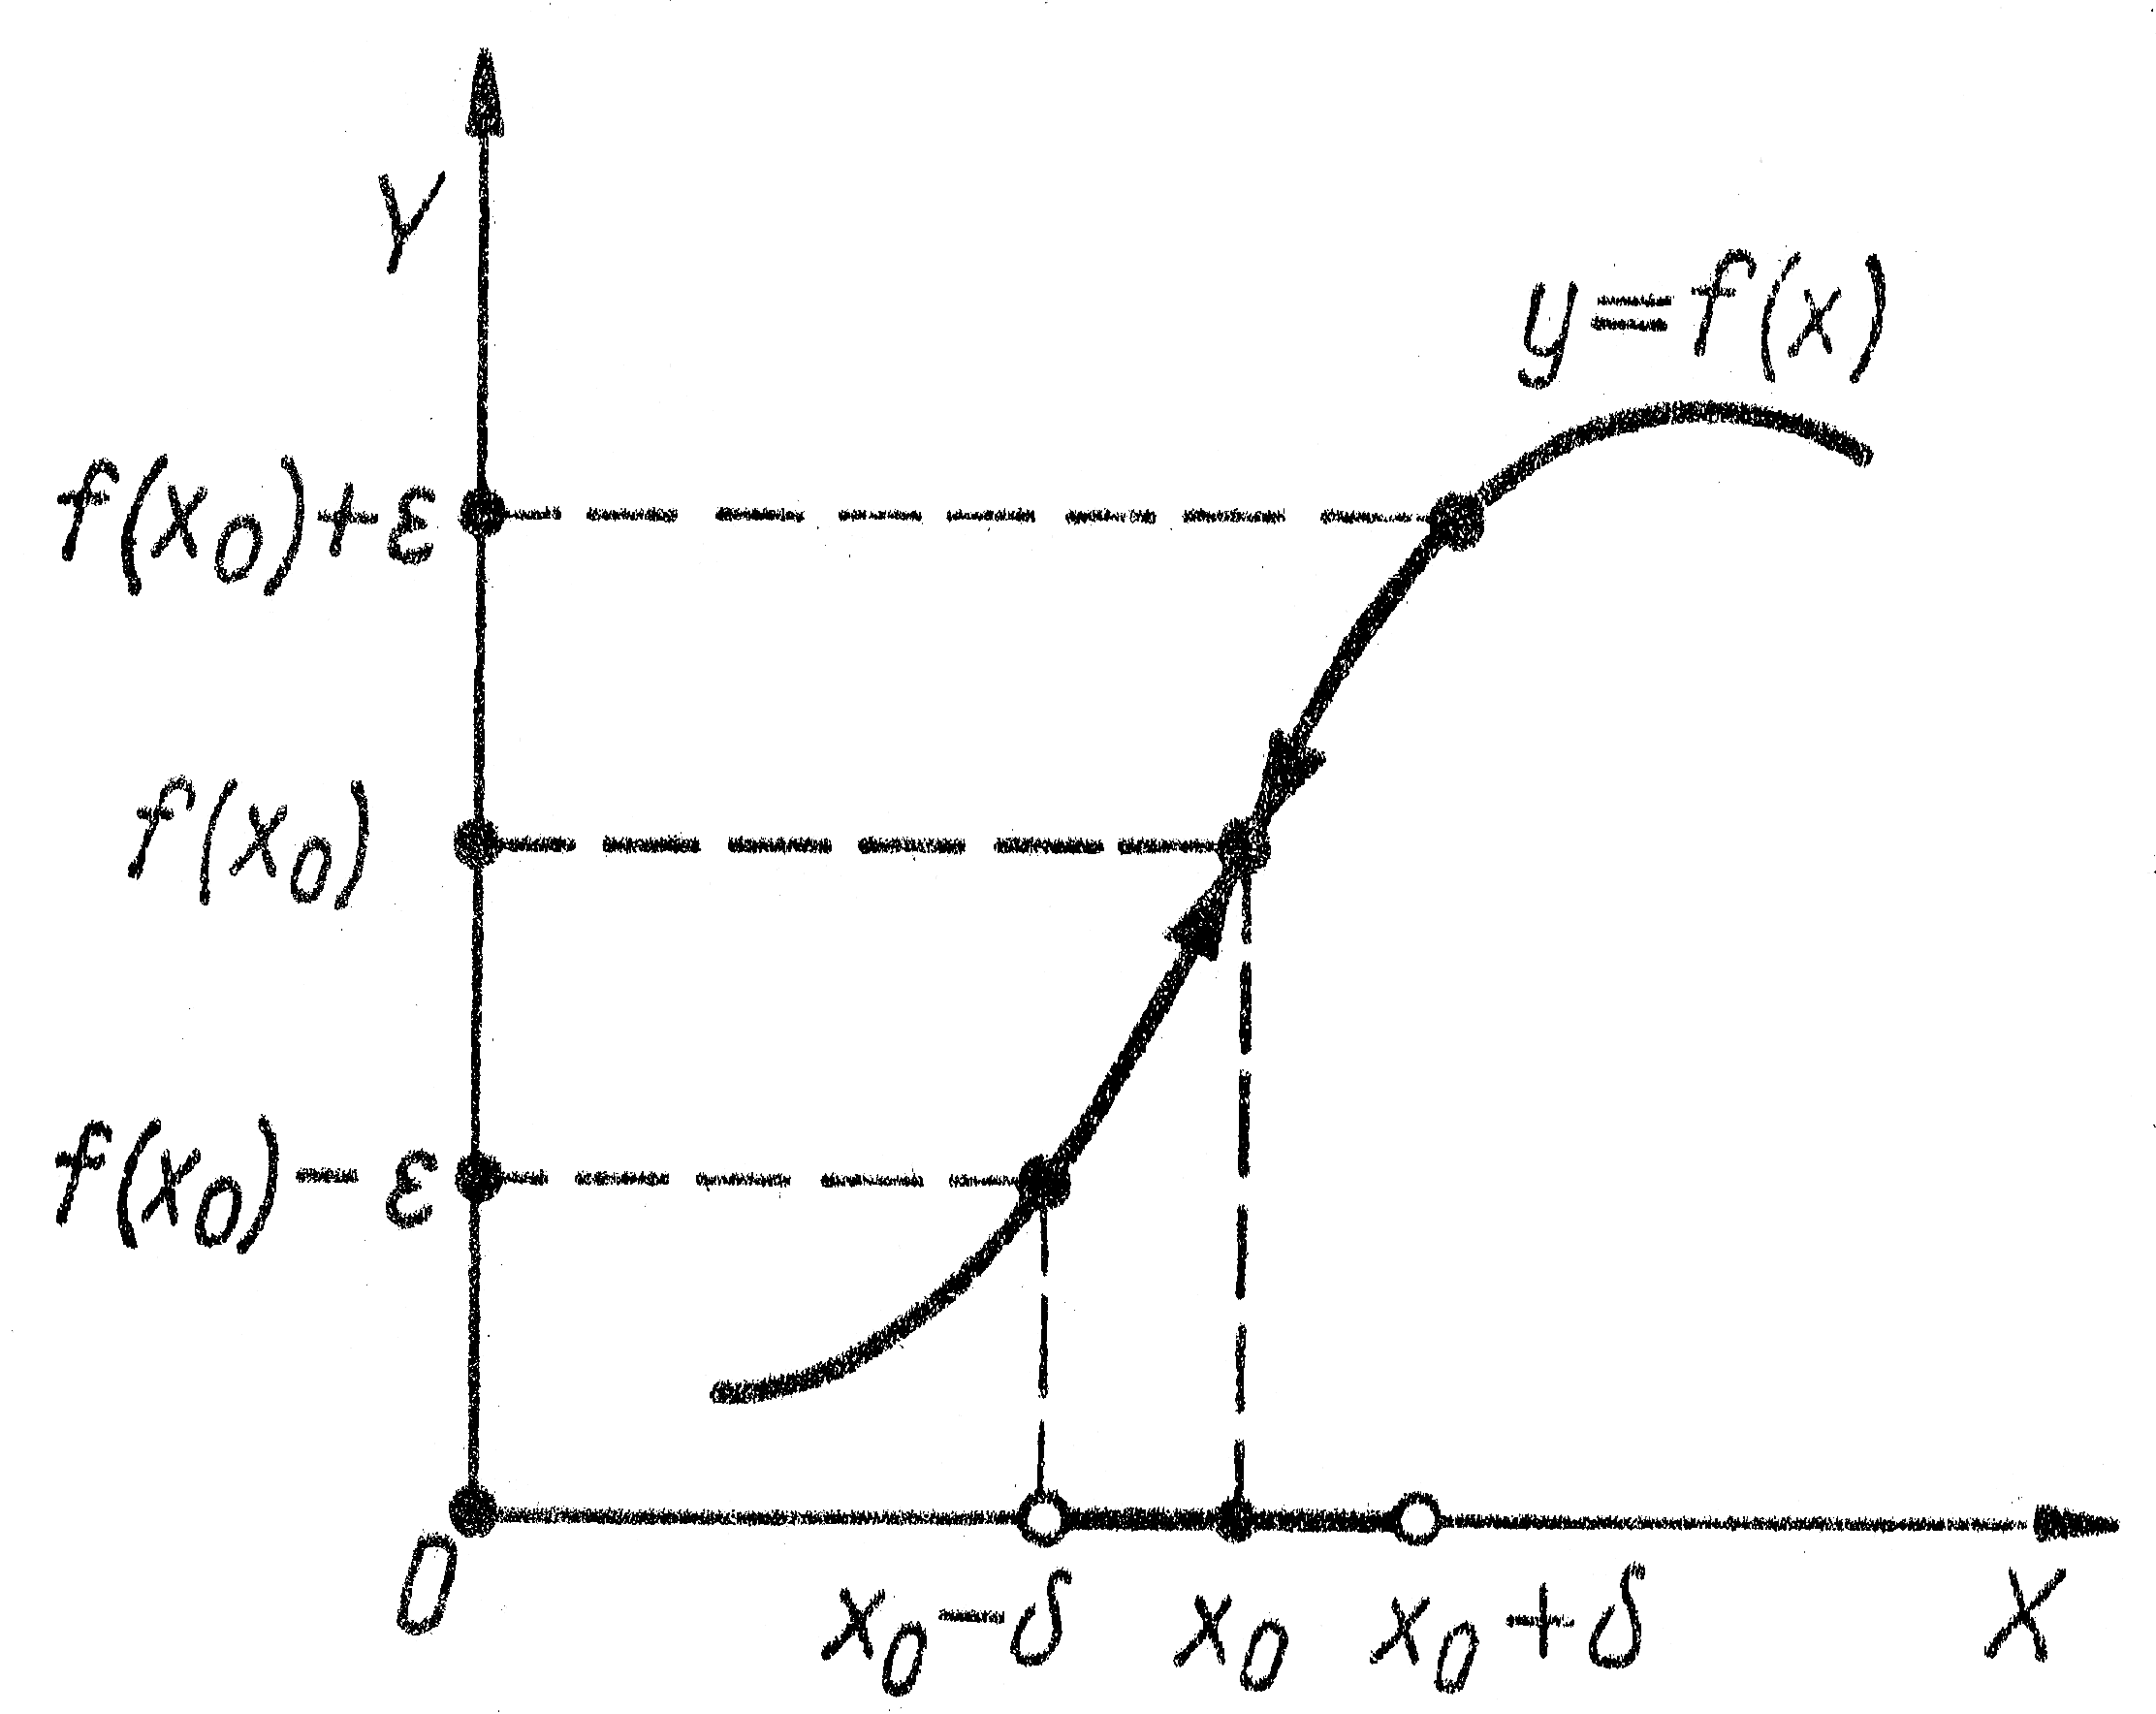
\includegraphics[scale=1.5]{img/funkcje-funkcja_ciagla.png}

\end{definicja}

\medskip
\cite[Rozdzia� 2.4]{zakowski1}


\bigskip
%%%%%%%%%%%%%%%%%%%%%%%%%%%%%%%%%%%%%%%%
\subsection{Definicja za pomoc� granicy}

\begin{twierdzenie}
Funkcj� $f(x)$ nazywamy \textbf{\emph{ci�g��}} w~punkcie $x_0$ wtedy i~tylko wtedy, gdy

\[ 
\exists \; \lim_{x \to x_0} f(x)
\]

oraz
\[
\lim_{x \to x_0} f(x) \quad = \quad f\left(x_0\right)
\]


\cite[Twierdzenie 5.36]{ptak} \cite[Paragraf 5.4]{krysicki1}
\end{twierdzenie}


\bigskip
%%%%%%%%%%%%%%%%%%%%%%%%%%%
\subsection{Funkcja ci�g�a}

\begin{definicja}
M�wimy, �e \textbf{\emph{funkcja}} $f$ jest \textbf{\emph{ci�g�a}}\label{def:funkcja_ciagla} wtedy i~tylko wtedy, gdy jest \textbf{ci�g�a w~ka�dym punkcie} (Def. \ref{def:funkcja_ciagla_w_punkcie}, str. \pageref{def:funkcja_ciagla_w_punkcie}) swej \textbf{dziedziny}.

\cite[Rozdzia� 2.4]{zakowski1}
\end{definicja}


\bigskip
%%%%%%%%%%%%%%%%%%%%%%%%%%%%%%%%%%%%%%
\subsection{Funkcja ci�g�a na zbiorze}

\begin{definicja}
M�wimy, �e \textbf{\emph{funkcja}} $f$ jest \textbf{\emph{ci�g�a na zbiorze}}\label{def:funkcja_ciagla_na_zbiorze} $A \subset D_f$ (TODO Df) wtedy i~tylko wtedy, gdy jest \textbf{ci�g�a w~ka�dym punkcie} (Def. \ref{def:funkcja_ciagla_w_punkcie}, str. \pageref{def:funkcja_ciagla_w_punkcie}) \textbf{zbioru} $A$.

\cite[Rozdzia� 2.4]{zakowski1}
\end{definicja}
\chapter{Rachunek r�niczkowy funkcji jednej zmiennej}

%%%%%%%%%%%%%%%%%%%%%%%%%%
\section{Pochodna funkcji}

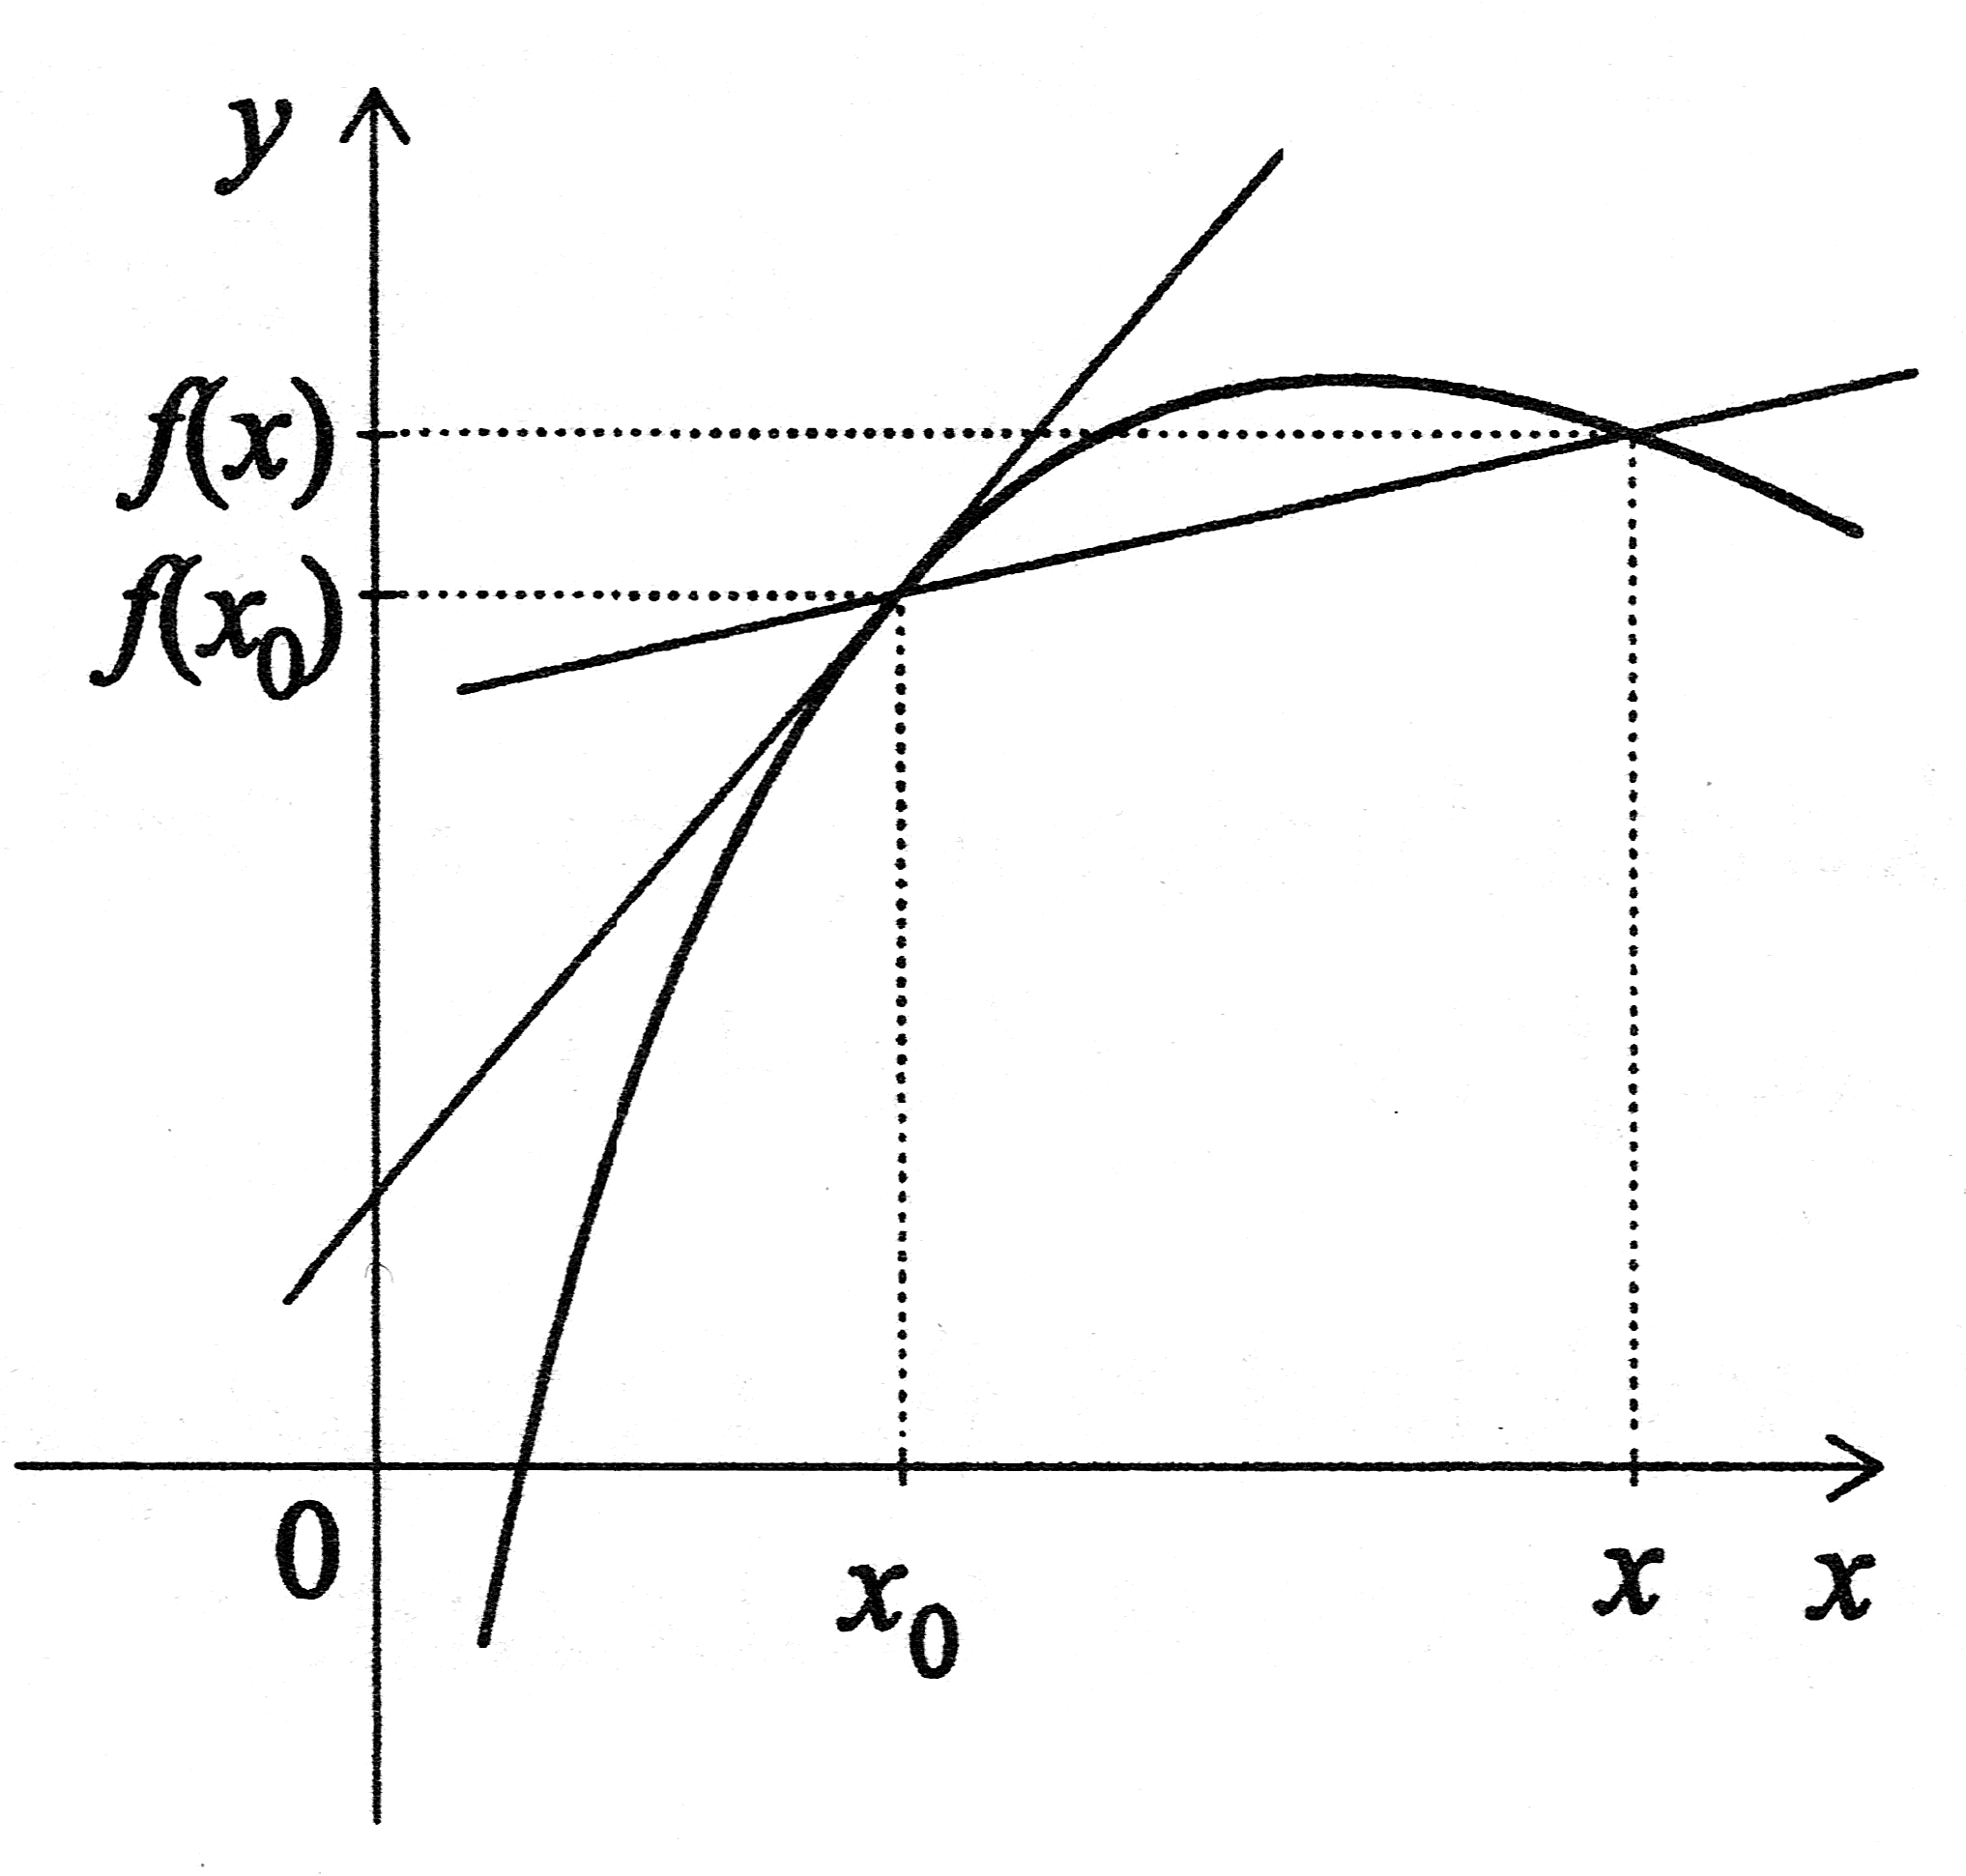
\includegraphics[scale=1.5]{img/pochodna-pochodna_funkcji.png}

\begin{definicja}
Funkcja
\[
f \colon (a,b) \to \mathbb{R}
\]
ma \textbf{\emph{pochodn� w punkcie $x_0$}}\label{def:pochodna_funkcji} wtedy i tylko wtedy, gdy

\[
\exists \lim_{x \to x_0} \dfrac{f(x) - f(x_0)}{x - x_0}
\]

\bigskip

Pochodn� funkcji oznaczamy
\[
y', \quad f'(x_0), \quad \dfrac{dy}{dx}, \quad \dfrac{df(x_0)}{dx}, \quad \dot y
\]

\medskip

czyli

\[
f'(x_0) = \lim_{x \to x_0} \dfrac{f(x) - f(x_0)}{x - x_0}
\]

\medskip

lub u�ywaj�c $h = x - x_0$

\[
f'(x_0) = \lim_{h \to 0} \dfrac{f(x_0+h) - f(x_0)}{h}
\]

\cite[Definicja 6.1]{ptak}
\end{definicja}

\bigskip
%%%%%%%%%%%%%%%%%%%%%%%%%%%%%%%%%
\subsection{Pochodna wy�szego rz�du}

\begin{definicja}
Niech funkcja $f \colon (a,b) \to \mathbb{R}$ b�dzie \textbf{r�niczkowalna} w~$(a,b)$, a~$x_0 \in (a,b)$.

\medskip

M�wimy, �e 
\begin{itemize}
\item $f$ jest \textbf{\emph{dwukrotnie r�niczkowalna}} w punkcie $x_0$,
\end{itemize}

\noindent lub �e

\begin{itemize}
\item $f$ ma \textbf{\emph{pochodn� drugiego rz�du}}\label{def:pochodna_drugiego_rzedu} w punkcie $x_0$,
\end{itemize}

\medskip

\noindent je�li
\begin{center}
funkcja $f' \colon (a,b) \to \mathbb{R}$ jest \textbf{r�niczkowalna} w $x_0$,
\end{center}

\medskip

\noindent co oznacza, �e

\[
\exists \left(f'\right)'(x_0) \quad \colon \quad f''(x_0) = \left(f'\right)'(x_0)
\]

\medskip

\cite[Definicja 6.36]{ptak} \cite[Rozdzia� 2.9]{zakowski1}
\end{definicja}

\bigskip

\begin{definicja}
Niech funkcja $f \colon (a,b) \to \mathbb{R}$ b�dzie \textbf{($n - 1$)-krotnie r�niczkowalna} w~$(a,b)$, a~$x_0 \in (a,b)$.

\medskip

M�wimy, �e 

\begin{itemize}
\item $f$ jest \textbf{\emph{$n$-krotnie r�niczkowalna}} w punkcie $x_0$,
\end{itemize}

\noindent lub �e

\begin{itemize}
\item $f$ ma \textbf{\emph{pochodn� $n$-tego rz�du}}\label{def:pochodna_n-tego_rzedu} w punkcie $x_0$,
\end{itemize}

\medskip

\noindent je�li

\begin{center}
funkcja $f^{(n-1)} \colon (a,b) \to \mathbb{R}$ jest \textbf{r�niczkowalna} w $x_0$,
\end{center}

\medskip

\noindent co oznacza, �e

\[
\exists \left(f^{(n-1)}\right)'(x_0) \quad \colon \quad f^{(n)}(x_0) = \left(f^{(n-1)}\right)'(x_0)
\]

\medskip

\cite[Definicja 6.37]{ptak} \cite[Rozdzia� 2.9]{zakowski1}
\end{definicja}

\bigskip
%%%%%%%%%%%%%%%%%%%%%%%%%%%%%%%%%%%%
\subsection{Interpretacja geometryczna}

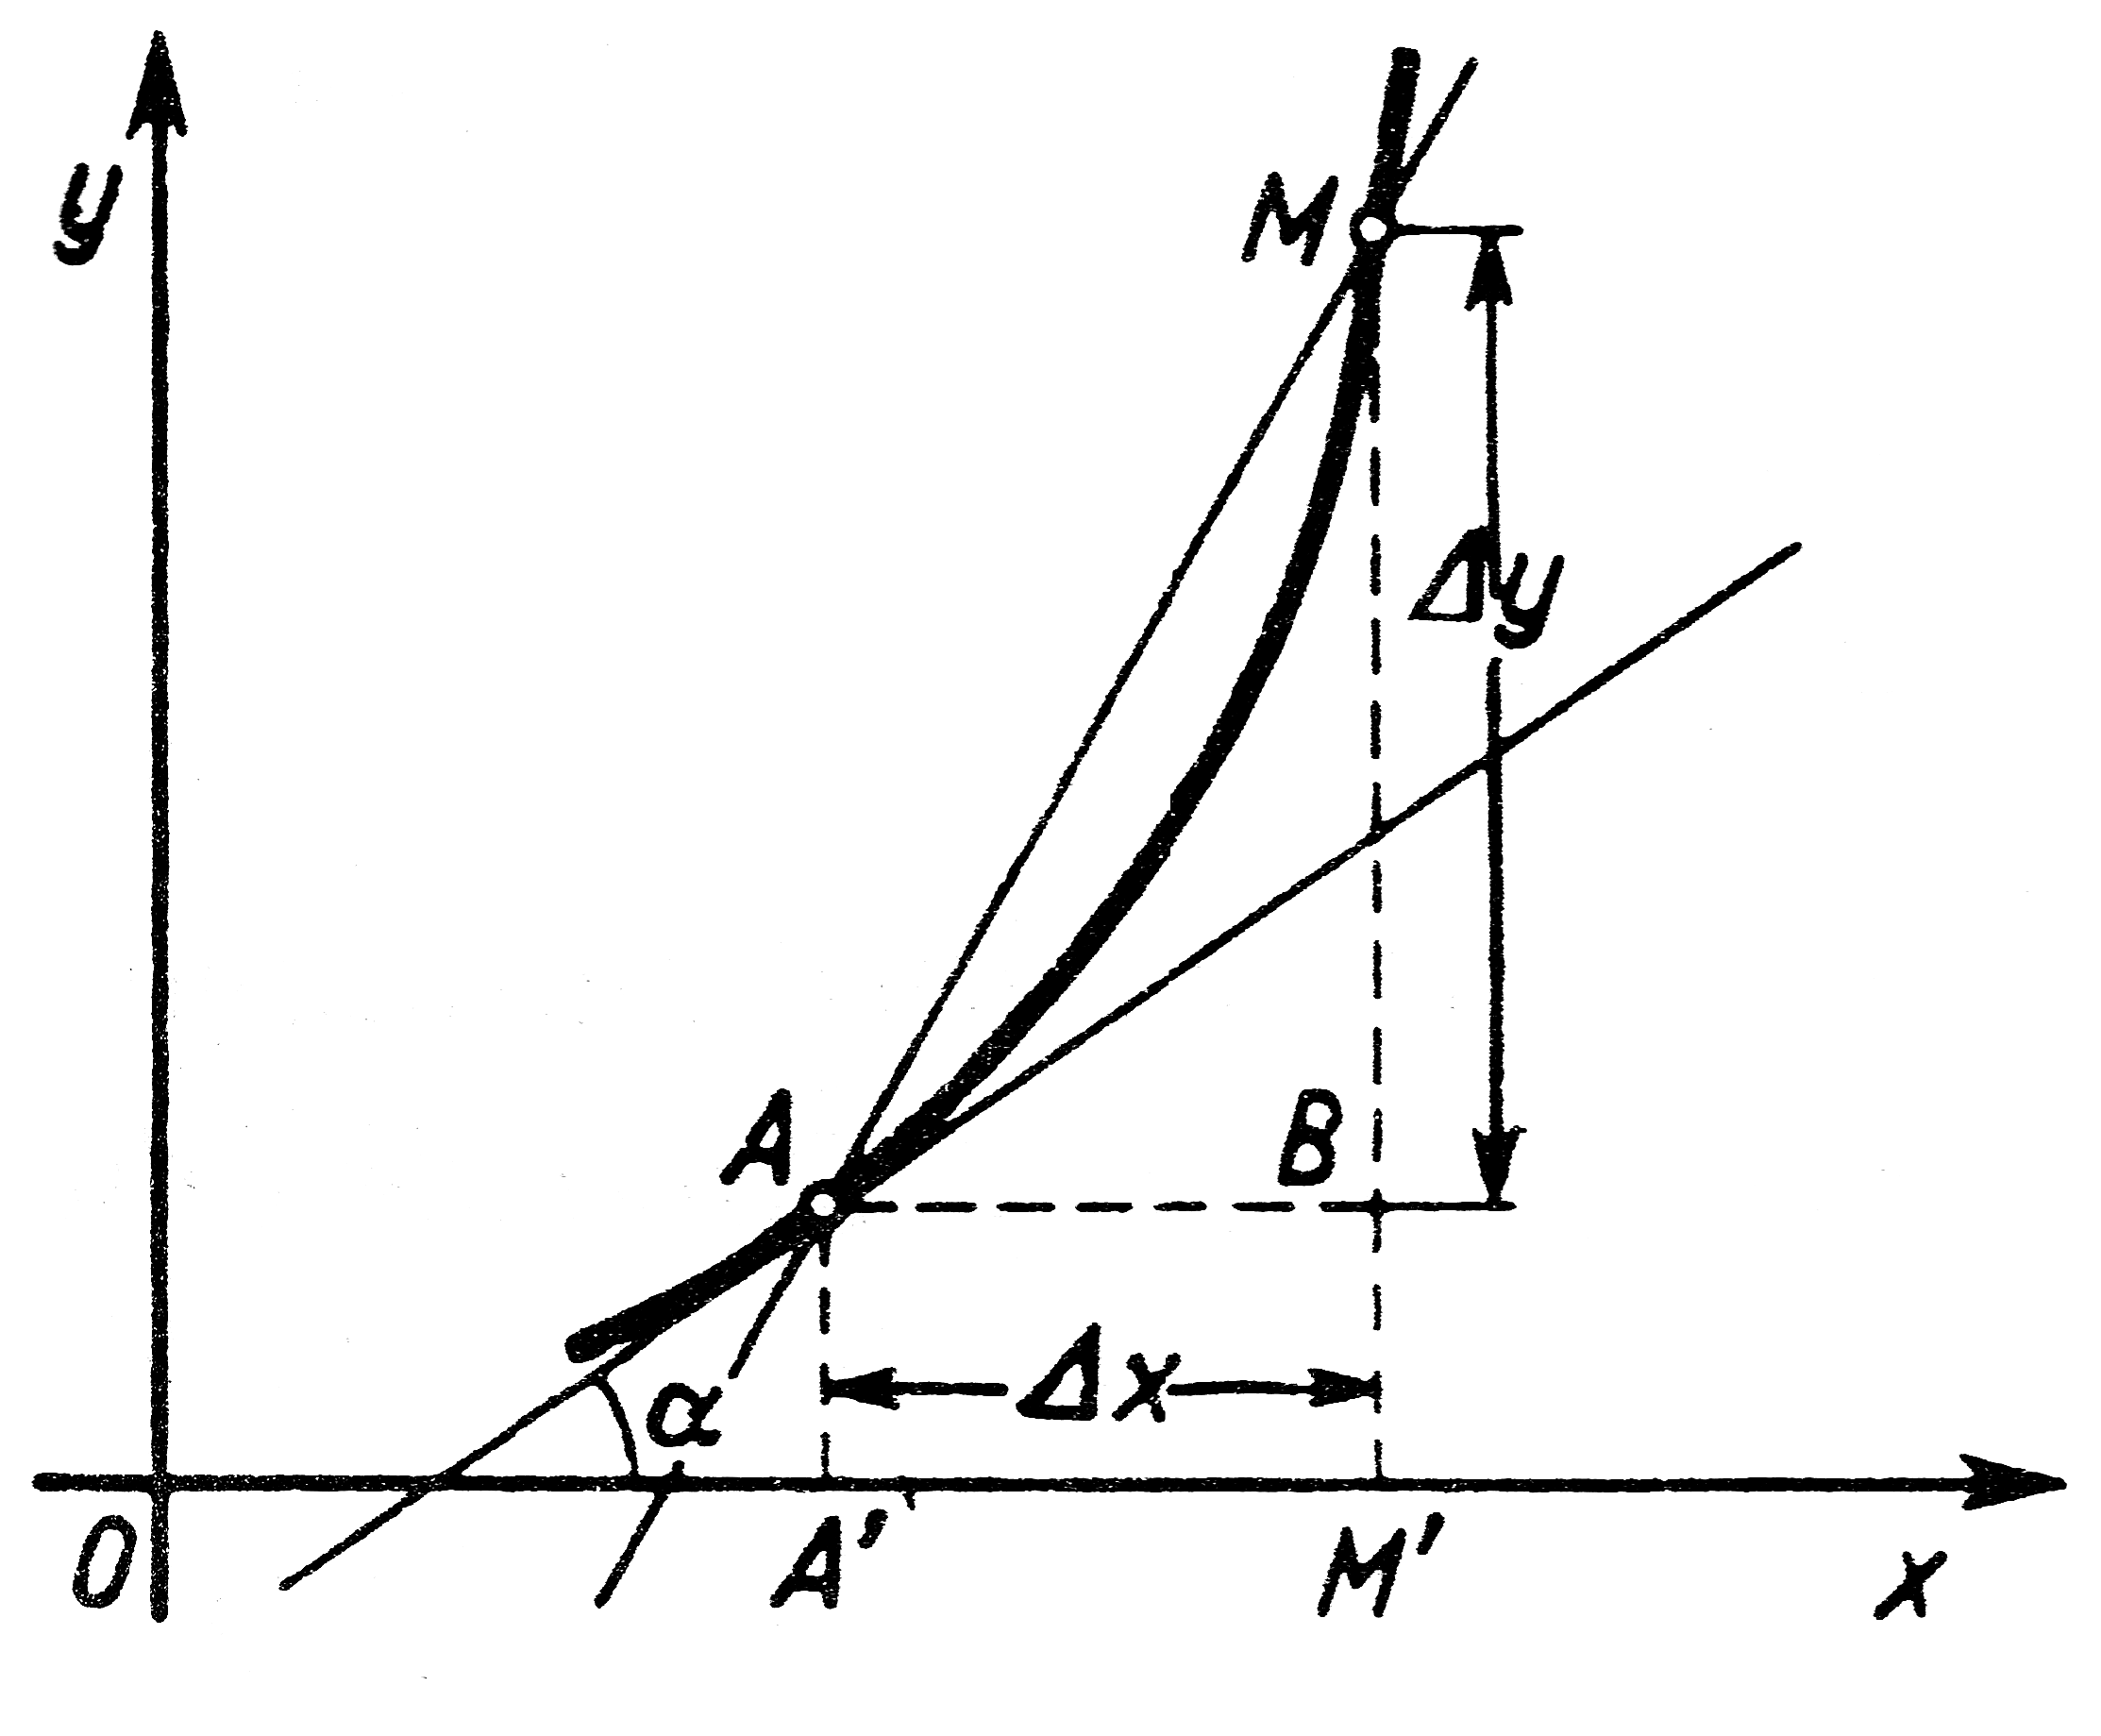
\includegraphics[scale=1.5]{img/pochodna-interpretacja_geometryczna.png}

Geometrycznie \textbf{\emph{pochodna}} funkcji $y = f(x)$ w punkcie $x_0$ r�wna si� \textbf{wp�czynnikowi k�towemu stycznej} (tangensowi k�ta $\alpha$, kt�ry prosta tworzy z dodatnim zwrotem osi $Ox$) do wykresu funkcji w tym punkcie.

\cite[Paragraf 6.1]{krysicki1}

\begin{twierdzenie}
Je�eli funkcja $f \colon (a,b) \to \mathbb{R}$ jest \textbf{r�niczkowalna} w $x_0 \in (a,b)$, to \textbf{styczna} do wykresu w punkcie $\left(x_0, f(x_0)\right)$ wyra�a si� wzorem:

\[
y - f(x_0) = f'(x_0)(x-x_0)
\]

\medskip

\cite[Wniosek 6.2]{ptak}
\end{twierdzenie}


%\bigskip
\newpage
%%%%%%%%%%%%%%%%%%%%%%%%%%%%%%
\subsection{Obliczanie pochodnej}

TODO marginesy

\[
\begin{array}{|rclc|l|}\hline
(c)' & = & 0 & \hspace{1cm} & c \textsl{ - sta�a} \\ \hline
(x)' & = & 1 & & \\ \hline
\left(x^a\right)' & = & a\;x^{a-1} & & x > 0, \quad a \in \mathbb{R}, \; a \neq 0 \\ \hline
\left(x^n\right)' & = & n\;x^{n-1} & & n \in \mathbb{N^+} \\ \hline
\left(\sqrt{x} \right)' & = & \dfrac{1}{2\sqrt{x}} & & x > 0 \\ \hline
\left(\dfrac{1}{x} \right)' & = & - \dfrac{1}{x^2} & & x \in \mathbb{R} \setminus \{0\} \\ \hline
\left(\sqrt[n]{x} \right)' & = & \dfrac{1}{n \; \sqrt[n]{x^{n-1}}} & & n \textsl{ - nieparzyste, } x \in \mathbb{R} \setminus \{0\} \\ \hline
\left(\sqrt[n]{x} \right)' & = & \dfrac{1}{n \; \sqrt[n]{x^{n-1}}} & & n \textsl{ - parzyste, } x > 0 \\ \hline
\left(\sin{x} \right)' & = & \cos{x} & &  \\ \hline
\left(\cos{x} \right)' & = & -\sin{x} & &  \\ \hline
\left(\tan{x} \right)' & = & \dfrac{1}{\cos^{2}{x}} & & x \in \mathbb{R} \setminus \left\{\frac{\pi}{2} + k\pi \colon k \in \mathbb{Z} \right\} \\ \hline
\left(\cot{x} \right)' & = & - \dfrac{1}{\sin^{2}{x}} & & x \in \mathbb{R} \setminus \left\{k\pi \colon k \in \mathbb{Z} \right\} \\ \hline
\left(\arcsin{x} \right)' & = & \dfrac{1}{\sqrt{1-x^2}} & & x \in (-1, 1) \\ \hline
\left(\arccos{x} \right)' & = & -\dfrac{1}{\sqrt{1-x^2}} & & x \in (-1, 1) \\ \hline
\left(\arctan{x} \right)' & = & \dfrac{1}{1 + x^2} & & x \in \left(-\frac{\pi}{2}, \frac{\pi}{2}\right) \\ \hline
\left(\arccot{x} \right)' & = & - \dfrac{1}{1 + x^2} & & x \in \left(0, \pi\right) \\ \hline
\left(\mathrm{e}^x \right)' & = & \mathrm{e}^x & &  \\ \hline
\left(\mathrm{a}^x \right)' & = & \mathrm{a}^x \; \ln{a} & & a > 0 \\ \hline
\left(\ln{x} \right)' & = & \dfrac{1}{x} & & x > 0 \\ \hline
\end{array}
\]

\cite[Paragraf 6.1]{krysicki1} \cite[Twierdzenie 6.13]{ptak} \cite[Rozdzia� 2.8, tabela 2.2a, 2.2b]{zakowski1}

\medskip

\begin{twierdzenie}[o dzia�aniach arytemtycznych na pochodnych]
Niech funkcje $f, g \colon (a,b) \to \mathbb{R}$ b�d� r�niczkowalne (Def. \ref{def:funkcja_rozniczkowalna}, str. \pageref{def:funkcja_rozniczkowalna}) w $x_0$, a $\lambda \in \mathbb{R}$. Wtedy

TODO odstepy

\[
\begin{array}{rcl}
\left(f \pm g\right)'\left(x_0\right) & = & f'\left(x_0\right) \pm g'\left(x_0\right) \\
\left(f \cdot g\right)'\left(x_0\right) & = & f'\left(x_0\right) g\left(x_0\right) + f\left(x_0\right) g'\left(x_0\right) \\
\left(\lambda \cdot f\right)'\left(x_0\right) & = & \lambda f'\left(x_0\right) \\
\left(\dfrac{f}{g}\right)'\left(x_0\right) & = & \dfrac{f'\left(x_0\right) g\left(x_0\right) - f\left(x_0\right) g'\left(x_0\right)}{g^2\left(x_0\right)}
\end{array}
\]
\cite[Twierdzenie 6.9]{ptak} \cite[Rozdzia� 2.8]{zakowski1}
\end{twierdzenie}

\bigskip

\begin{twierdzenie}[o pochodnej funkcji z�o�onej]
Niech b�d� dane dwie funkcje:

\[
\begin{array}{rlcl}
f \colon & (a,b) & \to & (c,d) \\
g \colon & (c,d) & \to & \mathbb{R}
\end{array}
\]

\medskip

Za��my, �e funkcja

\begin{itemize}
\item $f$ jest \textbf{r�niczkowalna} (Def. \ref{def:funkcja_rozniczkowalna}, str. \pageref{def:funkcja_rozniczkowalna}) w punkcie $x_0$
\item $g$ jest \textbf{r�niczkowalna} w punkcie $y_0 = f\left(x_0\right)$
\end{itemize}

\medskip

Wtedy funkcja $g \circ f\colon (a,b) \to \mathbb{R}$ jest \textbf{r�niczkowalna} w punkcie $x_0$

\[
\left(g \circ f\right)'\left(x_0\right) = g'\Big(f\left(x_0\right)\Big) \cdot f'\left(x_0\right)
\]

albo

\[
\bigg(g\Big(f\left(x_0\right)\Big)\bigg)' = g'\Big(f\left(x_0\right)\Big) \cdot f'\left(x_0\right)
\]

\medskip

\cite[Twierdzenie 6.10]{ptak} \cite[Rozdzia� 2.8]{zakowski1}
\end{twierdzenie}

\bigskip

\begin{twierdzenie}[o pochodnej funkcji odwrotnej]
Niech b�d� dane funkcje

\[
\begin{array}{rlcl}
f \colon & (a,b) & \to & (c,d) \\
f^{-1} \colon & (c,d) & \to & (a,b)
\end{array}
\]

\medskip

Za��my, �e funkcja

\begin{itemize}
\item $f$ jest odwracalna
\item $f^{-1}$ jest funkcj� odwrotn� (Def. \ref{def:relacja_odwrotna}, str. \pageref{def:relacja_odwrotna}) do $f$
\item $f$ jest \textbf{r�niczkowalna} (Def. \ref{def:funkcja_rozniczkowalna}, str. \pageref{def:funkcja_rozniczkowalna}) w punkcie $x_0$
\item $f^{-1}$ jest \textbf{ci�g�a} w punkcie $y_0 = f\left(x_0\right)$
\end{itemize}

\medskip

Wtedy funkcja $f^{-1}$ jest \textbf{r�niczkowalna} w punkcie $y_0$ oraz

\[
\left(f^{-1}\right)' \left(y_0\right) = \dfrac{1}{f'\left(x_0\right)}
\]

\medskip

\cite[Twierdzenie 6.11]{ptak} \cite[Rozdzia� 2.8]{zakowski1}
\end{twierdzenie}

\bigskip

\begin{definicja}
\textbf{\emph{Pochodn� logarytmiczn�}} funkcji $f$ nazywamy pochodn� jej logarytmu naturalnego

\[
\Big(\ln{f(x_0)}\Big)' = \dfrac{f'(x_0)}{f(x_0)}
\]

\medskip

Znaj�c ju� pochodn� logarytmiczn� funkcji mo�emy obliczy� jej pochodn�

\[
f'(x_0) = f(x_0) \cdot \Big(\ln{f(x_0)}\Big)'
\]

\medskip

\cite[Rozdzia� 2.8]{zakowski1}
\end{definicja}

\bigskip
%%%%%%%%%%%%%%%%%%%%%%%%%%%%%%%%%%
\subsection{Twierdzenia o pochodnych}

Niech $f \colon (a,b) \to \mathbb{R}$

\begin{twierdzenie}[r�niczkowalno�� a ci�g�o��]
Je�eli funkcja $f$ jest \textbf{r�niczkowalna} w $x_0 \in (a,b)$, to $f$ jest \textbf{ci�g�a} w $x_0$.
\end{twierdzenie}

\bigskip

\begin{twierdzenie}[o zwi�zku mi�dzy monotoniczno�ci� o pochodn�]
TODO
\end{twierdzenie}

%%%%%%%%%%%%%%%%%%%%%%%%%%%
\section{R�niczka funkcji}

\cite{zakowski1}[Rozdzia� 2.7]

%%%%%%%%%%%%%%%%%%%%%%%%%%%%%%%%%%%%%%%%%%%%%%%%%%%%%%%%%%%
\subsection{Twierdzenie o przedstawieniu przyrostu funkcji}

\begin{twierdzenie}[o przedstawieniu przyrostu funkcji]
Je�eli dziedzina funkcji $f$ zawiera pewne otoczenie $Q$ punktu $x_0$ oraz istnieje pochodna $f'(x_0)$, to dla ka�dego przyrostu $\Delta x$ takiego, �e $x_0 + \Delta x \in Q$, przyrost funkcji

\[
\Delta f = f\left(x_0 + \Delta x\right) - f\left(x_0\right)
\]

\medskip

mo�na przedstawi� nast�puj�co

\[
\Delta f = f'\left(x_0\right) \Delta x + \alpha \Delta x
\]

\medskip

przy czym $\alpha \to 0$, gdy $\Delta x$ d��y do zera w dowolny spos�b.

\medskip

\begin{proof}
Je�eli przyjmiemy

\[
\alpha = \left\{ \begin{array}{ccl}
\dfrac{\Delta f}{\Delta x} - f'(x_0) & \textsl{dla} & \Delta x \neq 0 \\
0 & \textsl{dla} & \Delta x = 0
\end{array} \right.
\]

\medskip

to dla ka�dego (dodatniego, ujemnego, b�d� r�wnego zeru) przyrostu $\Delta x$ takiego, �e $x_0 + \Delta x \in Q$, przedstawienie $\Delta f = f'\left(x_0\right) \Delta x + \alpha \Delta x$ jest prawdziwe.

Je�eli $\Delta x \to 0$, to poniewa� istnieje granica

\[
\lim_{\Delta x \to 0} \dfrac{\Delta f}{\Delta x} = f'\left(x_0\right)
\]

\medskip

wi�c wobec przyj�tego $\alpha$, $\alpha \to 0$, cnd.
\end{proof}
\end{twierdzenie}


\bigskip
%%%%%%%%%%%%%%%%%%%%%%%%%%%%%%%%%%%
\subsection{Funkcja r�niczkowalna}

\begin{definicja}
Funkcj� $f$ nazywamy \textbf{\emph{r�niczkowaln�}}\label{def:funkcja_rozniczkowalna} w punkcie $x_0$, je�eli jej przyrost 

\[
\Delta f = f\left(x_0 + \Delta x\right) - f\left(x_0\right)
\]

\medskip

mo�na dla ka�dego $\Delta x$ dostatecznie bliskiego zeru przedstawi� w postaci

\[
\Delta f = A \Delta x + o\left(\Delta x\right)
\]

\medskip

gdzie

\begin{itemize}
\item $A$ jest sta��,
\item a $o\left(\Delta x\right)$ jest niesko�czenie ma�� (Def. \ref{def:nieskonczenie_mala}, str. \pageref{def:nieskonczenie_mala}) rz�du wy�szego ni� $\Delta x$, gdy $\Delta x \to 0$.
\end{itemize}
\end{definicja}

\medskip

\emph{Wniosek}. Z twierdzenia o przedstawieniu przyrostu funkcji wynika, �e je�eli \textbf{istnieje} $f'(x_0)$, to funkcja $f$ jest w punkcie $x_0$ \textbf{r�niczkowalna}, przy czym $A = f'(x_0)$.

Na odwr�t, je�eli funkcja $f$ jest \textbf{r�niczkowalna} w punkcie $x_0$, to \textbf{istnieje} $f'(x_0) = A$.

\medskip

\emph{Wniosek}. Funkcja $f$ ma wi�c \textbf{pochodn�} w punkcie $x_0$ wtedy i tylko wtedy, gdy jest w tym punkcie \textbf{r�niczkowalna}, przy czym w�wczas

\[
\Delta f = f'\left(x_0\right) \Delta x + o\left(\Delta x\right)
\]

\medskip

dla ka�dego $\Delta x$ dostatecznie bliskiego zeru.

\bigskip
%%%%%%%%%%%%%%%%%%%%%%%%%%%%%%
\subsection{R�niczka funkcji}

\begin{definicja}
\textbf{\emph{R�niczk� funkcji}}\label{def:rozniczka_funkcji} $f$ w punkcie $x_0$ i dla przyrostu $\Delta x$ zmiennej niezale�nej $x$ nazywamy iloczyn

\[
f'(x_0) \Delta x
\]

\medskip

R�niczk� oznaczamy symbolem $df(x_0)$, b�d� te� kr�tko $df$ lub $dy$.

Mamy wi�c

\[
df(x_0) \; \stackrel{df}{=} \; f'(x_0) \Delta x
\]

lub kr�tko 

\[
dy \; \stackrel{df}{=} \; f'(x_0) \Delta x
\]
\end{definicja}


\bigskip
%%%%%%%%%%%%%%%%%%%%%%%%%%%%%%%%%%%%%%%%%%
\subsubsection{Interpretacja geometryczna}

\vspace{5cm}
TODO 2.24 str 106

\chapter{Badanie przebiegu zmienno�ci funkcji}

%%%%%%%%%%%%%%%%%%%%%%%%%%
\section{Ekstrema funkcji}

\cite{zakowski1}[Rozdzia� 2.13]

\medskip

\begin{definicja}
M�wimy, �e funkcja $f\colon \: (a,b) \to \mathbb{R}$ ma w punkcie $x_0 \in (a,b)$

\begin{itemize}
\item \textbf{\emph{maksimum lokalne}}\label{def:maksimum_lokalne}, je�li istnieje otoczenie punktu $x_0$ (Def. \ref{def:otoczenie_punktu}, str. \pageref{def:otoczenie_punktu}) takie, �e dla ka�dego $x$ z tego otoczenia mamy

\[
f(x_0) \geq f(x)
\]

\item \textbf{\emph{mocne maksimum lokalne}}\label{def:mocne_maksimum_lokalne}, je�li istnieje otoczenie punktu $x_0$ (Def. \ref{def:otoczenie_punktu}, str. \pageref{def:otoczenie_punktu}) takie, �e dla ka�dego $x$ z tego otoczenia oraz $x \neq x_0$ mamy

\[
f(x_0) > f(x)
\]

\item \textbf{\emph{minimum lokalne}}\label{def:minimum_lokalne}, je�li istnieje otoczenie punktu $x_0$ (Def. \ref{def:otoczenie_punktu}, str. \pageref{def:otoczenie_punktu}) takie, �e dla ka�dego $x$ z tego otoczenia mamy

\[
f(x_0) \leq f(x)
\]

\item \textbf{\emph{mocne minimum lokalne}}\label{def:mocne_minimum_lokalne}, je�li istnieje otoczenie punktu $x_0$ (Def. \ref{def:otoczenie_punktu}, str. \pageref{def:otoczenie_punktu}) takie, �e dla ka�dego $x$ z tego otoczenia oraz $x \neq x_0$ mamy

\[
f(x_0) < f(x)
\]
\end{itemize}

\vspace{5cm}
TODO rysunek 2.29, 2.30

\medskip

\cite{ptak}[Definicja 6.45]
\end{definicja}


\bigskip
%%%%%%%%%%%%%%%%%%%%%%%%%%%%%%%%%%%%%%%%%%%%%%%%%%
\subsection{Warunek konieczny istnienia ekstremum}

Niech $f\colon \: (a,b) \to \mathbb{R}$ b�dzie r�niczkowalna (Def. \ref{def:funkcja_rozniczkowalna}, str. \pageref{def:funkcja_rozniczkowlana}) w $x_0 \in (a,b)$.

\medskip

\begin{twierdzenie}[warunek konieczny istnienia ekstremum]
Je�li funkcja $f$ ma \textbf{maksimum} lokalne (\textbf{minimum} lokalne) w punkcie $x_0$, to 

\[
f'(x_0) = 0
\]

(Def. \ref{def:pochodna_funkcji}, str. \pageref{def:pochodna_funkcji}).

\medskip

\begin{proof}
Za��my, �e $f$ osi�ga \textbf{maksimum} lokalne w punkcie $x_0$.

\smallskip

Wtedy dla $x$ z otoczenia punktu $x_0$ (Def. \ref{def:otoczenie_punktu}, str. \pageref{def:otoczenie_punktu}) zachodzi nier�wno��:

\[
f(x) - f(x_0) \neq 0
\]

\medskip

Zatem dla $x_0 - \delta < x < x_0$ zachodzi nier�wno��

\[
\dfrac{f(x) - f(x_0)}{x - x_0} \geq 0
\]

\medskip

Poniewa� funkcja jest r�niczkowalna (Def. \ref{def:funkcja_rozniczkowalna}, str. \pageref{def:funkcja_rozniczkowlana}) w punkcie $x_0$, wi�c z twierdzenia o zachowaniu nier�wno�ci w granicy (Tw. \ref{tw:o_zachowaniu_nierownosci_w_granicy}, str. \pageref{tw:o_zachowaniu_nierownosci_w_granicy}) otrzymujemy:

\[
f'(x_0) = \lim_{x \to x_0} \dfrac{f(x) - f(x_0)}{x - x_0} \geq 0
\]

\medskip

Analogicznie, dla $x_0 < x < x_0 + \delta$ mamy

\[
\dfrac{f(x) - f(x_0)}{x - x_0} \leq 0
\]

\medskip

Rozumuj�c podobnie jak wy�ej, otrzymujemy

\[
f'(x_0) \leq 0
\]

\medskip

czyli

\[
f'(x_0) = 0
\]

\bigskip

Dow�d w przypadku \textbf{minimum} przebiega w taki sam spos�b.
\end{proof}

\medskip

\cite{ptak}[Twierdzenie 6.47]
\end{twierdzenie}

\vspace{5cm}
TODO rys. 2.32 str 132

\bigskip
%%%%%%%%%%%%%%%%%%%%%%%%%%%%%%%%%%%%%%%%%%%%%%%%%%%%%%%%
\subsection{Warunek wystarczaj�cy istnienia ekstremum I}

Niech $f\colon \: (a,b) \to \mathbb{R}$ b�dzie funkcj� klasy $C^{(2)}$ oraz $x_0 \in (a, b)$

\medskip

\begin{twierdzenie}[warunek wystarczaj�cy istnienia ekstremum lokalnego I]
Je�li $f'(x_0) = 0$ oraz

\begin{itemize}
\item $f''(x_0) < 0$, to $f$ ma mocne \textbf{maksimum} lokalne (Def. \ref{def:mocne_maksimum_lokalne}, str. \pageref{def:mocne_maksimum_lokalne}) w~punkcie $x_0$,
\item $f''(x_0) > 0$, to $f$ ma mocne \textbf{minimum} lokalne (Def. \ref{def:mocne_minimum_lokalne}, str. \pageref{def:mocne_minimum_lokalne}) w~punkcie $x_0$,
\end{itemize}

\begin{proof}
TODO sprawdzic, czy byl dowod na wykladzie
\end{proof}

\cite{ptak}[Twierdzenie 6.49]
\end{twierdzenie}

\bigskip
%%%%%%%%%%%%%%%%%%%%%%%%%%%%%%%%%%%%%%%%%%%%%%%%%%%%%%%%%
\subsection{Warunek wystarczaj�cy istnienia ekstremum II}

Niech $f\colon \: (a,b) \to \mathbb{R}$ b�dzie funkcj� klasy $C^{(1)}$ oraz $x_0 \in (a,b)$.

\medskip

\begin{twierdzenie}[warunek wystarczaj�cy istnienia ekstremum lokalnego II]
Je�li istnieje $\delta > 0$ takie, �e:

\begin{itemize}
\item 
\[
\begin{array}{lclrcll}
f'(x) > 0 & \textsl{dla} & x \in (& x_0 - \delta &,& x_0 &) \\
f'(x) < 0 & \textsl{dla} & x \in (& x_0 &,& x_0 + \delta &)
\end{array}
\]
(w skr�cie m�wimy, �e \textbf{pochodna} funkcji \textbf{zmienia znak} z \textbf{dodatniego} na \textbf{ujemny}), to $f$ ma mocne \textbf{maksimum} lokalne (Def. \ref{def:mocne_maksimum_lokalne}, str. \pageref{def:mocne_maksimum_lokalne}) w~punckie $x_0$.

\item 
\[
\begin{array}{lclrcll}
f'(x) < 0 & \textsl{dla} & x \in (& x_0 - \delta &,& x_0 &) \\
f'(x) > 0 & \textsl{dla} & x \in (& x_0 &,& x_0 + \delta &)
\end{array}
\]
(w skr�cie m�wimy, �e \textbf{pochodna} funkcji \textbf{zmienia znak} z \textbf{ujemnego} na \textbf{dodatni}), to $f$ ma mocne \textbf{minimum} lokalne (Def. \ref{def:mocne_minimum_lokalne}, str. \pageref{def:mocne_minimum_lokalne}) w~punckie $x_0$.

\end{itemize}

\medskip

\begin{proof}
TODO sprawdzic czy byl dowod na wykladzie
\end{proof}

\vspace{5cm}
TODO rys. 2.33 str 134

\medskip

\cite{ptak}[Twierdzenie 6.50]
\end{twierdzenie}


\bigskip
%%%%%%%%%%%%%%%%%%%%%%%%%%%%%
\section{Twierdzenie Rolle'a}

\bigskip
%%%%%%%%%%%%%%%%%%%%%%%%%%%%%%%%%%
\section{Twierdzenie Weierstrassa}

\bigskip
%%%%%%%%%%%%%%%%%%%%%%%%%%%%%%%%
\section{Twierdzenie Lagrange'a}

\bigskip
%%%%%%%%%%%%%%%%%%%%%%%%%%%%%
\section{Twierdzenie Taylora}

\bigskip
%%%%%%%%%%%%%%%%%%%%%%%%%%%%%%%%
\section{Twierdzenie Maclaurina}

\bigskip
%%%%%%%%%%%%%%%%%%%%%%%%%%%%%%%%%%%%%%%%%%%%%%%
\section{Wkl�s�o�� i wypuk�o�� wykresu funkcji}

\bigskip
%%%%%%%%%%%%%%%%%%%%%%%%%%
\section{Punkt przegi�cia}

\bigskip
%%%%%%%%%%%%%%%%%%%%%%%%%%%%%%%%%%%%%%%%%%%%%%%%%%%%%%%%%%
\subsection{Warunek konieczny istnienia punktu przegi�cia}

\bigskip
%%%%%%%%%%%%%%%%%%%%%%%%%%%%%%%%%%%%%%%%%%%%%%%%%%%%%%%%%%%%%%
\subsection{Warunek wystarczaj�cy istnienia punktu przegi�cia}

\bigskip
%%%%%%%%%%%%%%%%%%%
\section{Asymptoty}

\bigskip
%%%%%%%%%%%%%%%%%%%%
\subsection{Pionowa}

\bigskip
%%%%%%%%%%%%%%%%%%%%
\subsection{Pozioma}

\bigskip
%%%%%%%%%%%%%%%%%%%
\subsection{Uko�na}

\bigskip
%%%%%%%%%%%%%%%%%%%%%%%%%%%%%%%%%%%%%%%%%%%%%%%%%%%%%%
\section{Schemat badania przebiegu zmienno�ci funkcji}
\chapter{Rachunek ca�kowy funkcji jednej zmiennej}

%%%%%%%%%%%%%%%%%%%%%%%%%%%
\section{Funkcja pierwotna}

\begin{definicja}
\textbf{\emph{Funkcj� pierwotn�}}\label{def:funkcja_pierwotna}\index{funkcja!pierwotna} funkcji $f(x)$ w~przedziale $a < x < b$ nazywamy ka�d� tak� funkcj� $F(x)$, �e

\[
F'(x) \quad = \quad f(x)
\]

\medskip

dla ka�dego $x$ z~przedzia�u $a < x < b$.

\cite[Paragraf 15.1]{krysicki1} \cite[Rozdia� 3.4]{zakowski1}
\end{definicja}

\medskip

\begin{twierdzenie}
Je�eli $F(x)$ i $G(x)$ s� funkcjami pierwotnymi $f(x)$, to

\[
F(x) - G(x) \quad = \quad \textsl{const}
\]

(Dwie funkcje maj�ce w~danym przedziale t� sam� sko�czon� pochodn� \textbf{mog� si� r�ni� co najwy�ej o~sta��})

\cite[Paragraf 15.1]{krysicki1}
\end{twierdzenie}

\medskip

\begin{twierdzenie}[o istnieniu funkcji pierwotnej]
\label{tw:o_istnieniu_funkcji_pierwotnej}
Je�eli funkcja $f$ jest \textbf{ci�g�a} (jest klasy $C^0$) (Def. \ref{def:funkcja_ciagla_na_zbiorze}, str. \pageref{def:funkcja_ciagla_na_zbiorze}) na pewnym przedziale, to \textbf{posiada} na tym przedziale \textbf{funkcj� pierwotn�}.

\cite[Rozdzia� 3.4]{zakowski1}
\end{twierdzenie}


\bigskip

%%%%%%%%%%%%%%%%%%%%%%%%%%%%
\section{Ca�ka nieoznaczona}

\begin{definicja}
\textbf{\emph{Ca�k� nieoznaczon�}}\label{def:calka_nieoznaczona}\index{ca�ka!nieoznaczona} funkcji $f(x)$, oznaczon� symbolem

\[
\int f(x) \: \textnormal{d}x
\]

nazywamy wyra�enie

\[
F(x) + C
\]

gdzie
\begin{itemize}
\item $F(x)$ jest funkcj� pierwotn� funkcji f(x) (Def. \ref{def:funkcja_pierwotna}, str. \pageref{def:funkcja_pierwotna})
\item a $C$ jest dowoln� sta��.
\end{itemize}

Jest wi�c

\[
\int f(x) \: \textnormal{d}x \quad = \quad F(x) + C, \quad \textsl{gdzie} \quad F'(x) = f(x)
\]

\cite[Paragraf 15.1]{krysicki1} \cite[Rozdzia� 3.5]{zakowski1}
\end{definicja}

\medskip

Je�eli funkcja posiada na pewnym przedziale \textbf{funkcj� pierwotn�}, to m�wimy, �e \textbf{jest} ona na tym przedziale \textbf{ca�kowalna} (w~sensie Newtona).

\cite[Rozdzia� 3.4]{zakowski1}

\bigskip

Z powy�szego oraz twierdzenia [\ref{tw:o_istnieniu_funkcji_pierwotnej}, str. \pageref{tw:o_istnieniu_funkcji_pierwotnej}] wynika, �e

\smallskip

je�eli funkcja $f$ jest \textbf{ci�g�a} (Def. \ref{def:funkcja_ciagla_na_zbiorze}, str. \pageref{def:funkcja_ciagla_na_zbiorze}) na pewnym przedziale to jest \textbf{ca�kowalna} na tym przedziale.

\newpage

%%%%%%%%%%%%%%%%%%%%%%%%%%%%%%%%%%%%%%%%
\section{Obliczanie ca�ki nieoznaczonej}

%%%%%%%%%%%%%%%%%%%%%%%%%%%%%
\subsection{Podstawowe wzory}

\begin{center}
\begin{tabular}{|m{2cm}m{0,3cm}m{3cm}|m{3cm}|m{0,1cm}}
\cline{1-4}
 
$\int 0 \: \textnormal{d}x$ &
$=$ &
$C$ &
 &
 \\[10pt] \cline{1-4}
 
$\int x^a \: \textnormal{d}x$ &
$=$ &
$\dfrac{x^{a+1}}{a+1} + C$ &
$a \neq -1, \; x>0$ &
 \\[18pt] 
 
$\int \textnormal{d}x$ &
$=$ &
$x + C$ &
 &
 \\[10pt]
 
$\int\dfrac{\textnormal{d}x}{\sqrt{x}}$ &
$=$ &
$2\sqrt{x} + C$ &
$x>0$ &
 \\[15pt]
 
$\int \dfrac{\textnormal{d}x}{x^2}$ &
$=$ &
$-\dfrac{1}{x} + C$ &
$x \neq 0$ &
 \\[18pt] \cline{1-4}
 
$\int \dfrac{\textnormal{d}x}{x}$ &
$=$ &
$ln|x| + C$ &
$x \neq 0$ &
 \\[18pt] \cline{1-4}
 
$\int a^x \: \textnormal{d}x$ &
$=$ &
$\dfrac{a^x}{\ln a} + C$ &
$a>0, \: a \neq 1$ &
 \\[15pt]
 
$\int e^x \: \textnormal{d}x$ &
$=$ &
$e^x + C$ &
 &
 \\[10pt] \cline{1-4}
 
$\int \cos x \: \textnormal{d}x$ &
$=$ &
$\sin x + C$ &
 &
 \\[10pt] \cline{1-4}

$\int \sin x \: \textnormal{d}x$ &
$=$ &
$- \cos x + C$ &
 &
 \\[10pt] \cline{1-4}
  
$\int \dfrac{\textnormal{d}x}{\cos^2 x}$ &
$=$ &
$\tg x + C$ &
$\cos x \neq 0$ &
 \\[18pt] \cline{1-4}
  
$\int \dfrac{\textnormal{d}x}{\sin^2}$ &
$=$ &
$-\ctg x + C$ &
$\sin x \neq 0$ &
 \\[18pt] \cline{1-4}
 
$\int \dfrac{\textnormal{d}x}{\sqrt{1-x^2}}$ &
$=$ &
$\arcsin x + C$ &
$-1<x<1$ &
 \\[18pt] \cline{1-4}
 
$\int \dfrac{\textnormal{d}x}{\sqrt{1-x^2}}$ &
$=$ &
$- \arccos x + C$ &
$-1<x<1$ &
 \\[18pt] \cline{1-4}
 
   $\int \dfrac{\textnormal{d}x}{x^2 + 1}$ &
$=$ &
$\arc \tg x + C$ &
 &
 \\[18pt] \cline{1-4}
 
$\int \dfrac{\textnormal{d}x}{x^2 + 1}$ &
$=$ &
$-\arc \ctg x + C$ &
 &
 \\[18pt] \cline{1-4}
 
$\int \sinh x \: \textnormal{d}x$ &
$=$ &
$\cosh x + C$ &
 &
 \\[10pt] \cline{1-4}
 
$\int \cosh \: \textnormal{d}x$ &
$=$ &
$\sinh + C$ &
 &
 \\[10pt] \cline{1-4}
  
\end{tabular}
\end{center}

\cite[Paragraf 15.2]{krysicki1}

\bigskip

%%%%%%%%%%%%%%%%%%%%%%%%%%%%%%%%%%%%%%%%%%%
\subsection{W�asno�ci ca�ek nieoznaczonych}

\begin{twierdzenie}[o ca�ce sumy]\label{tw:o_calce_sumy}
Ca�ka sumy r�wna si� sumie ca�ek, tzn. (jest to tzw. addytywno�� ca�ki wzgl�dem funkcji podca�kowej)

\[
\int \Big(f(x) + g(x)\Big) \textnormal{d}x \quad = \quad \int f(x) \: \textnormal{d}x + \int g(x) \: \textnormal{d}x
\]

\cite[Paragraf 15.3, (15.3.1)]{krysicki1}
\end{twierdzenie}

\medskip

\begin{twierdzenie}\label{tw:o_wyniesieniu_stalego_czynnika_przed_znak_calki}
Sta�y czynnik wolno wynie�� przed znak ca�ki, tzn.

\[
\int A \: f(x) \: \textnormal{d}x \quad = \quad A \int f(x) \: \textnormal{d}x, \quad A \neq 0, \; A = \textsl{const}
\]

\cite[Paragraf 15.3, (15.3.2)]{krysicki1}
\end{twierdzenie}

\bigskip
%%%%%%%%%%%%%%%%%%%%%%%%%%%%%%%%%%%%
\subsection{Ca�kowanie przez cz�ci}

\begin{twierdzenie}[o ca�kowaniu przez cz�ci]\label{tw:o_calkowaniu_przez_czesci}
Je�eli funkcje $f(x)$ i~$g(x)$ maj� na pewnym przedziale ci�g�e pochodne $f'(x)$ i~$g'(x)$, to

\[
\int f'(x) \: g(x) \: \textnormal{d}x \quad = \quad f(x)\: g(x) - \int f(x) \: g'(x) \: \textnormal{d}x
\]

\medskip

na tym przedziale

\cite[Rozdzia� 3.6]{zakowski1}
\end{twierdzenie}

\bigskip
%%%%%%%%%%%%%%%%%%%%%%%%%%%%%%%%%%%%%%%%%%
\subsection{Ca�kowanie przez podstawienie}

\begin{twierdzenie}[o ca�kowaniu przez podstawienie]\label{tw:o_calkowaniu_przez_podstawienie}
Je�eli dla $a \: \leq \: x \: \leq \: b$

\begin{itemize}
\item $g(x) = u$ jest funkcj� maj�c� \textbf{ci�g�� pochodn�}
\item oraz $A \: \leq \: g(x) \: \leq \: B$,
\item a funkcja $f(u)$ jest \textbf{ci�g�a} w~przedziale $\langle A,B\rangle$
\end{itemize}

to

\[
\int f\Big(g(x)\Big) \: g'(x) \: \textnormal{d}x \quad = \quad \int f(u) \: du
\]

\medskip

przy czym po sca�kowaniu prawej strony nale�y w~otrzymanym wyniku podstawi� $u \: = \: g(x)$

\cite[Paragraf 15.3, (15.3.4)]{krysicki1}
\end{twierdzenie}

\bigskip
%%%%%%%%%%%%%%%%%%%%%%%%%%%%%%%%%%%%%
\subsection{Ca�ki funkcji wymiernych}

Ca�ka funkcji wymiernej (Def. \ref{def:funkcja_wymierna}, str. \pageref{def:funkcja_wymierna}), to ca�ka postaci

\[
\int \frac{P_n(x)}{Q_m(x)} \: \textnormal{d}x
\]

\medskip

\noindent Przy obliczaniu powy�szej ca�ki nale�y:

\begin{itemize}
\item je�eli funkcja wymierna jest \textbf{niew�a�ciwa}, czyli $m \geq n$ (Def. \ref{def:funkcja_wymierna_niewlasciwa}, str. \pageref{def:funkcja_wymierna_niewlasciwa}), to nale�y \textbf{podzieli� licznik przez mianownik} i~przedstawi� t� funkcj� jako \textbf{sum� wielomianu} oraz \textbf{funkcji wymiernej w�a�ciwej} (Tw. \ref{tw:funkcja_wymierna_suma_wielomianu_i_funkcji_wymiernej_wlasciwej}, str. \pageref{tw:funkcja_wymierna_suma_wielomianu_i_funkcji_wymiernej_wlasciwej}), czyli mamy

\[
\int \dfrac{P_p(x)}{Q_q(x)} \: \textnormal{d}x \quad = \quad \int \Big( W_w(x) \: + \: \dfrac{R_r(x)}{Q_q(x)} \Big) \: \textnormal{d}x
\]

\medskip

nast�pnie skorzysta� z~twierdzenia o~ca�ce sumy (Tw. \ref{tw:o_calce_sumy}, str. \pageref{tw:o_calce_sumy}), st�d mamy

\[
\int \dfrac{P_p(x)}{Q_q(x)} \: \textnormal{d}x \quad = \quad \int W_w(x) \: \textnormal{d}x \; + \; \int \dfrac{R_r(x)}{Q_q(x)} \: \textnormal{d}x
\]

\medskip

Pierwsz� ca�k� obliczamy korzystaj�c z~twierdzenia o~ca�ce sumy, z~twierdzenia o~wyniesieniu sta�ego czynnika przed znak ca�ki (Tw. \ref{tw:o_wyniesieniu_stalego_czynnika_przed_znak_calki}, str. \pageref{tw:o_wyniesieniu_stalego_czynnika_przed_znak_calki}) oraz podstawowych wzor�w na obliczanie ca�ki.

\smallskip

Drug� ca�k� obliczamy w~spos�b podany poni�ej.

\item je�eli funkcja wymierna jest \textbf{w�a�ciwa}, czyli $n < m$ (Def. \ref{def:funkcja_wymierna_wlasciwa}, str. \pageref{def:funkcja_wymierna_wlasciwa}), to przedstawiamy j� jako \textbf{sum� u�amk�w prostych} (Tw. \ref{tw:o_rozkladzie_na_ulamki_proste}, str. \pageref{tw:o_rozkladzie_na_ulamki_proste}).
\end{itemize}

\cite[Paragraf 16.1]{krysicki1}

\bigskip
%%%%%%%%%%%%%%%%%%%%%%%%%%%%%%%%%%%%%%%%%%%%%%%%%%%%%%%%%%%%%%
\subsubsection{Ca�kowanie u�amk�w prostych pierwszego rodzaju}

U�amki proste pierwszego rodzaju (Def. \ref{def:ulamek_prosty_pierwszego_rodzaju}, str. \pageref{def:ulamek_prosty_pierwszego_rodzaju}) ca�kujemy korzystaj�c z~twierdzenia o~ca�kowaniu przez podstawienie (Tw. \ref{tw:o_calkowaniu_przez_podstawienie}, str. \pageref{tw:o_calkowaniu_przez_podstawienie}) i~podstawienia

\[
u \quad = \quad x - a
\]

\medskip

st�d

\[
\int \frac{A}{(x - a)^n} \: \textnormal{d}x \quad = \quad A \int \frac{1}{u^n} \: du
\]

\medskip

i w ko�cu

\[
\int \frac{A}{(x - a)^n} \: \textnormal{d}x \quad = \quad \left\{ \begin{array}{cllc}
A & \ln |x-a| + C, & \textsl{gdy } r = 1 & \\[4pt]
\dfrac{A}{1-r} & (x-a)^{1-r} + C, &  \textsl{gdy TODO ?? ->} r \geq 2 &
\end{array} \right.
\]

\bigskip
%%%%%%%%%%%%%%%%%%%%%%%%%%%%%%%%%%%%%%%%%%%%%%%%%%%%%%%%%%%%%%
\subsubsection{Ca�kowanie u�amk�w prostych drugiego rodzaju}

U�amki proste drugiego rodzaju (Def. \ref{def:ulamek_prosty_drugiego_rodzaju}, str. \pageref{def:ulamek_prosty_drugiego_rodzaju}) ca�kujemy korzystaj�c, w~pierwszej kolejno�ci, z~twierdzenia o~ca�ce sumy (Tw. \ref{tw:o_calce_sumy}, str. \pageref{tw:o_calce_sumy}), z~twierdzenia o~wyniesieniu sta�ego czynnika przed znak ca�ki (Tw. \ref{tw:o_wyniesieniu_stalego_czynnika_przed_znak_calki}, str. \pageref{tw:o_wyniesieniu_stalego_czynnika_przed_znak_calki}), z~czego uzyskujemy dwie ca�ki

\begin{itemize}
\item pierwsz� postaci

\[
\int \frac{2x + p}{(x^2 +px + q)^n} \: \textnormal{d}x
\]

\medskip

gdzie licznik podca�kowej funkcji wymiernej ma posta� pochodnej funkcji mianownika b�d�cej w~pot�dze

\item drug� postaci

\[
\int \frac{1}{(x^2 +px + q)^n} \: \textnormal{d}x
\]

\end{itemize}

\bigskip

Aby otrzyma� te ca�ki licznik $Ax + B$ u�amka prostego przekszta�camy, w~og�lnym przypadku, nast�puj�co

\[
Ax + B \; = \; \frac{A}{2} \cdot 2x + B \; = \; \frac{A}{2} (2x + p - p) + B \; = \; \frac{A}{2} (2x + p) + B - \frac{Ap}{2}
\]

\bigskip

St�d do sca�kowania u�amka prostego drugiego rodzaju zastosujemy nast�puj�ce przekszta�cenie 

\[
\begin{array}{rcrlcc}
\int \dfrac{Ax + B}{(x^2 + px + q)^n} & = &  \dfrac{A}{2} & \int \dfrac{2x + p}{(x^2 +px + q)^n} \: \textnormal{d}x & + & \\[10pt]
& + & \left(B - \dfrac{Ap}{2}\right) & \int \dfrac{1}{(x^2 +px + q)^n} \: \textnormal{d}x & &
\end{array}
\]

\bigskip

Pierwsz� ca�k� 

\[
\int \frac{2x + p}{(x^2 +px + q)^n} \: \textnormal{d}x
\]

\medskip

obliczamy stosuj�c podstawienie 

\[
t \; = \; x^2 +px + q
\]

\medskip

st�d

\[
\textnormal{d}t \; = \; (2x + p) \: \textnormal{d}x
\]

\medskip

Otrzymujemy wi�c

\[
\int \frac{2x + p}{(x^2 +px + q)^n} \: \textnormal{d}x \quad = \quad \int \frac{1}{t^n} \: \textnormal{d}t
\]

\medskip

Dalsze ca�kowanie przebiega tak, jak w~przypadku u�amka prostego.

\bigskip

Drug� ca�k�

\[
\int \frac{1}{(x^2 +px + q)^n} \: \textnormal{d}x
\]

\medskip

przekszta�camy tak, aby otrzyma�

\[
\int \frac{1}{(t^2 + 1)^n} \: \textnormal{d}t
\]

\medskip


w~og�lnym przypadku stosuj�c podstawienie

\[
t \; = \; \frac{2x +p}{\sqrt{-\Delta}}
\]

\cite[Rozdzia� 3.8]{zakowski1}

\bigskip

Ca�k� 

\[
\int \frac{1}{(t^2 + 1)^n} \: \textnormal{d}t
\]

dla 

\begin{itemize}
\item $n = 1$ rozwi�zujemy korzystaj�c z podstawowych wzor�w ca�kowania

\[
\int \frac{1}{t^2 + 1} \: \textnormal{d}t \; = \; \arc \tg{t} + C
\]

\item $n > 1$ rozwi�zujemy korzystaj�c ze \textbf{wzoru redukuj�cego} (lub \textbf{rekurencyjnego})

\[
I_n = \frac{1}{2n-2} \cdot \frac{t}{(t^2 + 1)^{n-1}} + \frac{2n-3}{2n-2} \; I_{n-1}, \qquad \textsl{gdzie } I_n = \int \frac{1}{(t^2 + 1)^n} \: \textnormal{d}t
\]

\medskip

kt�rego wyprowadzenie znajduje si� poni�ej.

\bigskip

\textbf{Wyprowadzenie}

\medskip

Aby obliczy� ca�k�

\[
I_n = \int \frac{1}{(t^2 + 1)^n} \: \textnormal{d}t
\]

\medskip

zastosujemy przekszta�cenie

\[
\int \frac{1}{(t^2 + 1)^n} \: \textnormal{d}t \; = \; \int \frac{t^2 + 1 - t^2}{(t^2 + 1)^n} \: \textnormal{d}t \; =
\]

\[
 = \; \int \frac{1}{(t^2 + 1)^{n-1}} \: \textnormal{d}t \; - \; \int \frac{t^2}{(t^2 + 1)^n} \: \textnormal{d}t
\]

\medskip

czyli mamy

\[
I_n \; = \; I_{n-1} \; - \; \int \frac{t^2}{(t^2 + 1)^n} \: \textnormal{d}t
\]

\medskip

Drug� ca�k� zapisujemy jako

\[
\int \frac{t^2}{(t^2 + 1)^n} \: \textnormal{d}t \; = \; \int t \cdot \frac{t}{(t^2 + 1)^n} \: \textnormal{d}t
\]

\medskip

i~ca�kujemy przez cz�ci (Tw. \ref{tw:o_calkowaniu_przez_czesci}, str. \pageref{tw:o_calkowaniu_przez_czesci}). St�d otrzymujemy

\[
\int \frac{t^2}{(t^2 + 1)^n} \: \textnormal{d}t \; = \; \frac{-1}{2n -2} \cdot \frac{t}{(t^2 +1)^{n-1}} + \frac{1}{2n-2} \; I_{n-1}
\]

\medskip

Po podstawieniu do wzoru na $I_n$ otrzymujemy zapisany wy�ej \textbf{wz�r redukcyjny}.

\cite[Zadanie 16.21]{krysicki1}
\end{itemize}

\bigskip
%%%%%%%%%%%%%%%%%%%%%%%%%%%%%%%%%%%%%%%%%%%%%
\subsection{Ca�ki funkcji trygonometrycznych}

Ca�ki trygonometryczne obliczamy stosuj�c podstawienia charakterystyczne dla danych typ�w.

\begin{itemize}
\item 
\[
\int R(\sin x) \cos x \: \textnormal{d}x
\]

\begin{eqnarray*}
t 	& = & \sin x \\
\textnormal{d}t	& = & \cos x \: \textnormal{d}x
\end{eqnarray*}

\item

\[
\int R(\cos x) \sin x \: \textnormal{d}x
\]

\begin{eqnarray*}
t 	& = & \cos x \\
- \textnormal{d}t	& = & \sin x \: \textnormal{d}x
\end{eqnarray*}

\item

\[
\int R(\sin^2 x, \cos^2 x, \sin x \cos x) \: \textnormal{d}x
\]

\begin{eqnarray*}
t 							& = & \tg x \\
\arc \tg t					& = & x \\
\frac{1}{1 + t^2} \: \textnormal{d}t		& = & \textnormal{d}x
\end{eqnarray*}

\[
\sin^2 x \; = \; \frac{\sin^2 x}{1} \; = \; \frac{\sin^2 x}{\cos^2 x + \sin^2 x} \; = \; \frac{\tg^2 x}{1 + \tg^2 x} \; = \; \frac{t^2}{1 + t^2}
\]

\[
\cos^2 x \; = \; \frac{\cos^2 x}{1} \; = \; \frac{\cos^2 x}{\cos^2 x + \sin^2 x} \; = \; \frac{1}{1 + \tg^2 x} \; = \; \frac{1}{1 + t^2}
\]

\[
\sin x \cos x \; = \; \frac{\sin x \cos x}{1} \; = \; \frac{\sin x \cos x}{\cos^2 x + \sin^2 x} \; = \; \frac{\tg x}{1 + \tg^2 x} \; = \; \frac{t}{1 + t^2}
\]

\item

\[
\int R(\sin x, \cos x) \: \textnormal{d}x
\]

\begin{eqnarray*}
t 							& = & \tg \frac{x}{2} \\
\arc \tg t					& = & \frac{x}{2} \\
\frac{2}{1 + t^2} \: \textnormal{d}t		& = & \textnormal{d}x
\end{eqnarray*}

\[
\sin x \; = \; \frac{2 \sin \frac{x}{2} \cos \frac{x}{2}}{1} \; = \; \frac{2 \sin \frac{x}{2} \cos \frac{x}{2}}{\cos^2 \frac{x}{2} + \sin^2 \frac{x}{2}} \; = \; \frac{2 \tg \frac{x}{2}}{1 + \tg^2 \frac{x}{2}} \; = \; \frac{2t}{1 + t^2}
\]

\[
\cos x \; = \; \frac{\cos^2 \frac{x}{2} - \sin^2 \frac{x}{2}}{1} \; = \; \frac{\cos^2 \frac{x}{2} - \sin^2 \frac{x}{2}}{\cos^2 \frac{x}{2} + \sin^2 \frac{x}{2}} \; = \; \frac{1 - \tg^2 \frac{x}{2}}{1 + \tg^2 \frac{x}{2}} \; = \; \frac{1 - t^2}{1 + t^2}
\]
\end{itemize}

\bigskip
%%%%%%%%%%%%%%%%%%%%%%%%%%%%%%%%%%%%%%%%
\subsection{Ca�ki funkcji niewymiernych}

\subsubsection{Ca�ki funkcji zawieraj�cych pierwiastki z~wyra�enia liniowego}

\cite[Paragraf 17.1]{krysicki1}

\medskip

Je�eli funkcja podca�kowa jest funkcj� wymiern� pot�g zmiennej $x$~o~wyk�adnikach postaci $\dfrac{m}{n}$, gdzie $m$, $n$ s� liczbami naturalnymi wzgl�dem siebie pierwszymi, to wykonujemy podstawienie

\[
x \; = \; t^N
\]

\medskip

gdzie $N$ oznacza wsp�lny mianownik u�amk�w postaci $\dfrac{m}{n}$.

\bigskip
%%%%%%%%%%%%%%%%%%%%%%%%%%%%%%%%%%%%%%%%%%%%%%%%%%%%%%%%%%%%%%%%%%%%%%%%%%%%%%%%%%%%%%%%%%%%%%%%%%%%%%%%%%%%%%%%%
\subsubsection{Podstawienia Eulera - Ca�ki funkcji zawieraj�cych pierwiastek kwadratowy z~tr�jmianu kwadratowego}

Ca�k� postaci

\[
\int R\left(x, \sqrt{ax^2 + bx +c}\right) \: \textnormal{d}x
\]

\medskip

mo�emy obliczy� stosuj�c \textbf{podstawienie Eulera}. W~zale�no�ci od warunk�w stosujemy podstawienia:

\begin{enumerate}
\item gdy $a \; > \; 0$

\[
\sqrt{ax^2 + bx +c} \; = \; t \pm \sqrt{a} \: x
\]

\medskip

\item gdy $\Delta = b^2 -4ac \; > \; 0 \qquad \Big(ax^2 + bx +c \; = \; a(x-x_1)(x-x_2)\Big)$

\[
\sqrt{ax^2 + bx +c} \; = \; (x-x_{1})t
\]

\medskip

lub

\[
\sqrt{ax^2 + bx +c} \; = \; (x-x_{2})t
\]
\end{enumerate}

\medskip

R�wnania podnosimy obustronnie do kwadratu. Obliczamy $x$ i~wstawiamy do podstawienia. Otrzymujemy w~ten spos�b podstawienie dla $\sqrt{ax^2 + bx +c}$ zale�ne jedynie od $t$. R�wnanie z~wyliczonym $x$ r�niczkujemy.

\bigskip
%%%%%%%%%%%%%%%%%%%%%%%%%%%%%%%%%%%%%%%%%%%%%%%%%%%%%%%%%%%%%%%%%%%%%%%%%%%
\subsubsection{Ca�kowanie przy pomocy metody wsp�czynnik�w nieoznaczonych}

\cite[Paragraf 17.3, Zadanie 17.46, 17.47]{krysicki1}

\medskip

\textbf{Metod� wsp�czynnik�w nieoznaczonych} stosujemy przy obliczaniu ca�ek postaci

\[
\int \frac{W_n(x)}{\sqrt{ax^2 + bx +c}} \: \textnormal{d}x
\]

\medskip

gdzie $W_n(x)$ jest wielomianem (Def. \ref{def:wielomian}, str. \pageref{def:wielomian}) stopnia $n$ (Def. \ref{def:stopien_wielomianu}, str. \pageref{def:stopien_wielomianu}). Ca�ka ta r�wna si� wyra�eniu

\[
W_{n-1}(x) \: \sqrt{ax^2 + bx +c} \; + \; A \int \frac{1}{\sqrt{ax^2 + bx +c}} \: \textnormal{d}x
\]

\medskip

gdzie $W_{n-1}(x)$ jest wielomianem stopnia $n-1$, a $A$ - pewn� sta��.

\bigskip

\noindent Aby obliczy� \textbf{wsp�czynniki (nieoznaczone) wielomianu} $W_{n-1}$ oraz~$\mathbf{A}$

\begin{enumerate}
\item r�niczkujemy obie strony to�samo�ci


\begin{align*}
\int \frac{W_n(x)}{\sqrt{ax^2 + bx +c}} \: \textnormal{d}x \; \equiv \; W_{n-1}(x) \: \sqrt{ax^2 + bx +c} \; + \\
+ \; A \int \frac{1}{\sqrt{ax^2 + bx +c}} \: \textnormal{d}x
\end{align*}

\medskip

otrzymujemy

\begin{align*}
\frac{W_n(x)}{\sqrt{ax^2 + bx +c}} \; \equiv \; W_{n-1}'(x) \: \sqrt{ax^2 + bx +c} \; + \\
+ \; W_{n-1}(x) \: \frac{2ax + b}{2\sqrt{ax^2 + bx +c}} \; + \\
+ \; A \: \frac{1}{\sqrt{ax^2 + bx +c}}
\end{align*}

\item mno�ymy obie strony to�samo�ci przez $\sqrt{ax^2 + bx +c}$

\[
W_n(x) \; \equiv \; W_{n-1}'(x) \: (ax^2 + bx +c) \; + \; W_{n-1}(x) \: \frac{2ax + b}{2} \; + \; A
\]

\item korzystaj�c z~(Tw. \ref{tw:rownosc_wielomianow}, str. \pageref{tw:rownosc_wielomianow}) przyr�wnujemy kolejno odpowiednie wsp�czynniki.
\end{enumerate}

\medskip

Obliczone wsp�czynniki wstawiamy do pierwotnej to�samo�ci i~obliczamy ca�k�

\[
\int \frac{1}{\sqrt{ax^2 + bx +c}} \: \textnormal{d}x
\]

\medskip

Otrzymany wynik wstawiamy do to�samo�ci. W~ten spos�b otrzymujemy warto�� pierwotnej ca�ki.

\bigskip
%%%%%%%%%%%%%%%%%%%%%%%%%%%%%%%%%%%%%%%
\subsubsection{Inne rodzaje podstawie�}

\begin{itemize}
\item

\[
\int R(x, \sqrt{a^2 - x^2}) \: \textnormal{d}x
\]

\[
x \; = \; a \: \sin t \quad \vee \quad x = a \: \tgh t
\]

\item

\[
\int R(x, \sqrt{a^2 + x^2}) \: \textnormal{d}x
\]

\[
x \; = \; a \: \tg t \quad \vee \quad x = a \: \sinh t
\]

\item

\[
\int R(x, \sqrt{x^2 - a^2}) \: \textnormal{d}x
\]

\[
x \; = \; \frac{a}{\cos t} \quad \vee \quad x = a \: \cosh t
\]

\end{itemize}

\bigskip
%%%%%%%%%%%%%%%%%%%%%%%%%
\section{Ca�ka oznaczona}

Zak�adamy, �e funkcja $f(x)$ jest ograniczona w~przedziale domkni�tym $\langle a,b\rangle$ (Def. \ref{def:funkcja_ograniczona_w_przedziale}, str. \pageref{def:funkcja_ograniczona_w_przedziale})

\vspace{5cm}

TODO rysunek konstrukcji

\bigskip

Dokonajmy nast�puj�cej konstrukcji:

\begin{itemize}
\item dokonujemy $m$ r�nych podzia��w ($P_1$, $P_2$, $\ldots$, $P_m$) przedzia�u $\langle a,b\rangle$ na cz�ci (dzielimy w~r�ny spos�b przedzia� $\langle a,b\rangle$ na mniejsze przedzia�y)

\item przyjmujemy, �e w~wyniku \textbf{podzia�u $\mathbf{P_m}$ otrzymali�my przedzia�y}

\[
\langle x_{i-1} , x_{i} \rangle, \qquad \textsl{gdzie } n = 1, 2, \ldots n_m
\]

gdzie

\begin{itemize}
\item $n_m$ - liczba przedzia��w
\item $x_0 = a$
\item $x_{n_m} = b$
\item liczby $x_i$ tworz� ci�g silnie rosn�cy (Def. \ref{def:ciag_silnie_rosnacy}, str. \pageref{def:ciag_silnie_rosnacy})
\end{itemize}

\medskip

Przedzia�y te nazywamy \textbf{przedzia�ami cz�stkowymi podzia�u} $P_m$.

\item oznaczamy d�ugo�ci przedzia��w

\[
x_i - x_{i-1} \; = \; \Delta x_i
\]

\item oznaczamy \textbf{d�ugo�� najd�u�szego przedzia�u cz�stkowego} podzia�u $P_m$ przez $\mathbf{\delta_m}$

\[
\delta_m \; = \; \sup{\Delta x_i}
\]

\item Ci�g (Def. \ref{def:ciag}, str. \pageref{def:ciag}) podzia��w $\{P_m\}$ nazywamy \textbf{normalnym ci�giem podzia��w}, je�eli

\[
\lim_{n \to \infty} \delta_m = 0
\]

\item tworzymy \textbf{sum� $\mathbf{S_m}$ iloczyn�w}
\begin{itemize}
\item \textbf{warto�ci funkcji} $\mathbf{f(c_i)}$ w~dowolnym punkcie $c_i$ przedzia�u $\langle x_{i-1} , x_{i} \rangle$
\item oraz \textbf{d�ugo�ci} $\mathbf{\Delta x_i}$ tych przedzia��w
\end{itemize}

przy podziale $P_m$

\[
S_m \; = \; \sum_{i=1}^{n_m} \: f(c_i) \: \Delta x_i
\]

\end{itemize}

\begin{definicja}
Je�eli

\begin{itemize}
\item \textbf{ci�g} $\mathbf{\{S_m\}}$ dla $m \to \infty$ jest \textbf{zbie�ny} (Def. \ref{def:ciag_zbiezny}, str. \pageref{def:ciag_zbiezny})
\item \textbf{i}, dodatkowo, jest \textbf{zbie�ny do tej samej granicy} przy \textbf{ka�dym} normalnym normalnym ci�gu podzia��w $\{P_m\}$, niezale�nie od wyboru punkt�w $c_i$,
\end{itemize}

\noindent to funkcj� $f(x)$ nazywamy \textbf{funkcj� ca�kowaln� w~przedziale} $\langle a,b\rangle$, a~granic� ci�gu $S_m$ nazywamy \textbf{ca�k� oznaczon�}\index{ca�ka!oznaczona} funkcji $f(x)$ \textbf{w~granicach od $a$ do $b$} i~oznaczamy symbolem

\[
\int\limits_a^b f(x) \: \textnormal{d}x
\]


\end{definicja}

\cite[Paragraf 19.1]{krysicki1}

\bigskip
%%%%%%%%%%%%%%%%%%%%%%%%%%%%%%%%%%%%%%%%%%%%%%%%%%%%%%%%
\subsection{Interpretacja geometryczna ca�ki oznaczonej}

\vspace{5cm}

TODO rysunek

\bigskip

\begin{twierdzenie}
Je�eli w przedziale $\langle a,b\rangle$ jest

\[
f \geq 0
\]

\medskip

\noindent to \textbf{pole obszaru} ograniczonego

\begin{itemize}
\item �ukiem krzywej $y = f(x)$,
\item odcinkiem osi $Ox$
\item prost� $x=a$
\item prost� $x=b$
\end{itemize}

\noindent r�wna si� ca�ce oznaczonej

\[
\int\limits_a^b f(x) \: \textnormal{d}x
\]

\cite[Paragraf 19.2]{krysicki1}

\end{twierdzenie}

\medskip

\noindent\textbf{Wniosek}

Je�eli w~przedziale $\langle a,b\rangle$ jest

\[
f \leq 0
\]

\medskip

to pole r�wna si� 

\[
- \int\limits_a^b f(x) \: \textnormal{d}x
\]

\bigskip

\noindent\textbf{Wniosek}

Zawsze pole okre�lonego wy�ej obszaru mo�na wyrazi� ca�k� oznaczon�\label{wn:pole_obszaru_ogolnie}

\[
\int\limits_a^b |f(x)| \: \textnormal{d}x
\]

\cite[Paragraf 19.2]{krysicki1}

\bigskip
%%%%%%%%%%%%%%%%%%%%%%%%%%%%%%%%%%%%%%%
\subsection{W�asno�ci ca�ki oznaczonej}

\cite[Paragraf 19.3]{krysicki1}

\bigskip
%%%%%%%%%%%%%%%%%%%%%%%%%%%%%%%%%%%%%%%%%%%%%%%%%%%%%%%%%%%%%%%%
\subsubsection{Addytywno�� ca�ki wzgl�dem przedzia�u ca�kowania}

\begin{twierdzenie}
Je�eli $a \leq b \leq c$, to (TODO niekonieczne za�o�enie)

\[
\int\limits_a^c f(x) \: \textnormal{d}x \quad = \quad \int\limits_a^b f(x) \: \textnormal{d}x + \int\limits_b^c f(x) \: \textnormal{d}x
\]
\end{twierdzenie}

\bigskip
%%%%%%%%%%%%%%%%%%%%%%%%%%%%%%%%%%%%%%%%%%%%%%%%%%%%%%%%%%%%%%
\subsubsection{Addytywno�� ca�ki wzgl�dem funkcji podca�kowej}

\begin{twierdzenie}
Ca�ka sumy r�wna si� sumie ca�ek, tzn.

\[
\int\limits_a^b \Big(f(x)+g(x)\Big) \: \textnormal{d}x \quad = \quad \int\limits_a^b f(x) \: \textnormal{d}x + \int\limits_a^b g(x) \: \textnormal{d}x
\]
\end{twierdzenie}

\bigskip
%%%%%%%%%%%%%%%%%%%%%%%%%%%%%%%%%%%%%%%%%%%%%%%%%%%%%%%%%%%%%%%%%%%%%%%
\subsubsection{Wynoszenie sta�ego czynnika przed znak ca�ki oznaczonej}

\begin{twierdzenie}
Sta�y czynnik mo�na wynie�� przed znak ca�ki

\[
\int\limits_a^b A \: f(x) \: \textnormal{d}x \quad = \quad A \: \int\limits_a^b f(x) \: \textnormal{d}x
\]
\end{twierdzenie}

\bigskip
%%%%%%%%%%%%%%%%%%%%%%%%%%%%%%%%%%%%%%%%%%%%%%%%%%%%%%%%%%%%%%
\subsubsection{Parzysto�� i~nieparzysto�� funkcji podca�kowej}

\begin{twierdzenie}
Je�eli $f(x) \in C^0 \Big(\langle -a,a\rangle\Big)$ i~jest nieparzysta (Def. \ref{def:funkcja_nieparzysta}, str. \pageref{def:funkcja_nieparzysta}), to

\[
\int\limits_{-a}^a f(x) \: \textnormal{d}x \quad = \quad 0
\]
\end{twierdzenie}

\medskip

\begin{twierdzenie}
Je�eli $f(x) \in C^0 \Big(\langle -a,a\rangle\Big)$ i~jest parzysta (Def. \ref{def:funkcja_parzysta}, str. \pageref{def:funkcja_parzysta}), to

\[
\int\limits_{-a}^a f(x) \: \textnormal{d}x \quad = \quad 2 \: \int\limits_0^a f(x) \: \textnormal{d}x \;
\]
\end{twierdzenie}

\bigskip
%%%%%%%%%%%%%%%%%%%%%%%%%%%%%%%%%%%%%%%%%%%%%%%%%%%%%%%%%%%%%%%%%%
\subsubsection{Twierdzenie o warto�ci �redniej}

\begin{twierdzenie}
Je�eli $f(x) \in C^0 \Big(\langle a,b\rangle\Big)$, to istnieje $c \in (a,b)$ takie, �e

\[
\int\limits_a^b f(x) \: \textnormal{d}x \quad = \quad f(c)(b-a)
\]
\end{twierdzenie}

\bigskip
%%%%%%%%%%%%%%%%%%%%%%%%%%%%%%%%%%%%%%%%%%%%%%%%%%%%%%%%%%%%%
\subsubsection{Zwi�zek mi�dzy ca�k� oznaczon� a~nieoznaczon�}

\begin{twierdzenie}
Je�eli przez $F(x)$ oznaczymy funkcj� pierwotn� (Def. \ref{def:funkcja_pierwotna}, str. \pageref{def:funkcja_pierwotna}) funkcji $f(x) \in C^0 \Big(\langle a,b\rangle\Big)$, to

\[
\int\limits_a^b f(x) \: \textnormal{d}x \quad = \quad F(b) - F(a)
\]
\end{twierdzenie}

\medskip

\noindent\textbf{Oznaczenia}

$F(b) - F(a)$ oznacza� mo�na przez

\begin{itemize}
\item $\big[F(x)\big]_a^b$
\item $F(x)|_a^b$
\item $F(x)|_{x=a}^{x=b}$
\end{itemize}

\bigskip
%%%%%%%%%%%%%%%%%%%%%%%%%%%%%%%%%%%%%%%%%%%%%%%%%%%%%%%%%
\subsubsection{Ca�kowanie przez cz�ci ca�ek oznaczonych}

\begin{twierdzenie}
Je�eli $f(x), g(x) \in C^1 \Big(\langle a,b\rangle\Big)$, to

\[
\int\limits_a^b f'(x) \: g(x) \: \textnormal{d}x \quad = \quad \big[f(x) \: g(x)\big]_a^b - \int\limits_a^b f(x) \: g'(x) \: \textnormal{d}x
\]
\end{twierdzenie}

\bigskip
%%%%%%%%%%%%%%%%%%%%%%%%%%%%%%%%%%%%%%%%%%%%%%%%%%%%%%%%%%%%%%%
\subsubsection{Ca�kowanie przez podstawienie ca�ek oznaczonych}

\begin{twierdzenie}\label{tw:o_calkowaniu_przez_podstawienie_calek_oznaczonych}
Je�eli 
\begin{itemize}
\item $g'(x)$ jest funkcj� ci�g�� (Def. \ref{def:funkcja_ciagla}, str. \pageref{def:funkcja_ciagla}),
\item $g(x)$ jest funkcj� silnie rosn�c� (Def. \ref{def:funkcja_silnie_rosnaca}, str. \pageref{def:funkcja_silnie_rosnaca}) w~przedziale $\langle a,b\rangle$
\item $f(t)$ jest ci�g�a w~przedziale $\Big\langle g(a), g(b)\Big\rangle$ (Def. \ref{def:funkcja_ciagla_na_zbiorze}, str. \pageref{def:funkcja_ciagla_na_zbiorze})
\end{itemize}

\medskip

to

\[
\int\limits_a^b f\Big(g(x)\Big) \: g'(x) \: \textnormal{d}x \quad = \quad \int\limits_{g(a)}^{g(b)} f(t) \: \textnormal{d}t
\]

\medskip

Podstawienie

\[
t \; = \; g(x)
\]

\end{twierdzenie}


\bigskip
%%%%%%%%%%%%%%%%%%%%%%%%%%%%%%%%%%%%%%%%%%
\subsection{Zastosowanie ca�ki oznaczonej}

\bigskip
%%%%%%%%%%%%%%%%%%%%%%%%%%%%%%%%%%%%%%%%%%%%%%%%%
\subsubsection{Obliczanie pola obszaru p�askiego}

TODO

\bigskip
%%%%%%%%%%%%%%%%%%%%%%%%%%%%%%%%%%%%%%%%%%%%%%%%%%%%%%%%%%%%%%%%%%%%%%%%%%%%%%%%%%%%%%%%%%%%%%%%%%%%%%%%%%%%%%%%%%
\subsubsection{Obliczanie pola obszaru p�askiego, gdy linia ograniczaj�ca okre�lona jest w~postaci parametrycznej}

\cite[Paragraf 20.1]{krysicki1}

\medskip

Je�eli linia ograniczaj�ca okre�lona jest w~\textbf{postaci parametrycznej}

\[
\begin{array}{rcl}
x & = & g(t)\\[4pt]
y & = & h(t)
\end{array}
\]

\medskip

\noindent gdzie w~przedziale $\langle t_1, t_2\rangle$

\begin{itemize}
\item funkcje $g(t)$ i~$h(t)$ s� \textbf{ci�g�e} (Def. \ref{def:funkcja_ciagla_na_zbiorze}, str. \pageref{def:funkcja_ciagla_na_zbiorze}) 
\item funkcja $g(t)$ jest \textbf{rosn�ca} (Def. \ref{def:funkcja_rosnaca}, str. \pageref{def:funkcja_rosnaca})
\item funkcja $g(t)$ ma \textbf{pochodn�} (Def. \ref{def:pochodna_funkcji}, str. \pageref{def:pochodna_funkcji})  \textbf{ci�g��} 
\end{itemize}

\bigskip

\noindent to, korzystaj�c z~(Tw. \ref{tw:o_calkowaniu_przez_podstawienie_calek_oznaczonych}, str. \pageref{tw:o_calkowaniu_przez_podstawienie_calek_oznaczonych}) oraz wniosk�w z~interpretacji geometrycznej ca�ki oznaczonej (Wn. \ref{wn:pole_obszaru_ogolnie}, str. \pageref{wn:pole_obszaru_ogolnie}), \textbf{pole obszaru} ograniczonego:

\begin{itemize}
\item dan� lini� ograniczaj�c� ($x \; = \; g(t)$, $y \; = \; h(t)$)
\item odcinkiem osi $Ox$
\item prost� $x \; = \; x_1$ ($x_1 \; = \; g(t_1)$)
\item prost� $x \; = \; x_2$ ($x_2 \; = \; g(t_2)$)
\end{itemize}

\medskip

\noindent wyra�a si� wzorem

\[
P \quad = \quad \int\limits_{x_1}^{x_2} |y| \: \textnormal{d}x \quad = \quad \int\limits_{t_1}^{t_2} |h(t)| \: g'(t) \: \textnormal{d}t
\]

\bigskip

\noindent W~przypadku, gdy

\begin{itemize}
\item za�o�enia s� \textbf{takie same} jak powy�ej
\item a funkcja $g(t)$ jest \textbf{malej�ca}
\end{itemize}

\medskip

\noindent to \textbf{pole obszaru} wyra�a si� 

\[
P \quad = \quad \int\limits_{x_1}^{x_2} |y| \: \textnormal{d}x \quad = \quad -\int\limits_{t_1}^{t_2} |h(t)| \: g'(t) \: \textnormal{d}t
\]

\bigskip
%%%%%%%%%%%%%%%%%%%%%%%%%%%%%%%%%%%%%%%%%%%%%%%%%%%%%%%%%%%%%%%%%%%%%%%%%%%%%%%%%%%%%%%%%%%%%%%%%%%%%%%%%%%%%%%%%%
\subsubsection{Obliczanie pola obszaru p�askiego, gdy linia ograniczaj�ca okre�lona jest we wsp�rz�dnych biegunowych}

\cite[Paragraf 20.1]{krysicki1}

\medskip

Je�eli linia ograniczaj�ca dana jest we wsp�rz�dnych biegunowych (Def. \ref{def:uklad_wspolrzednych_biegunowych}, str. \pageref{def:uklad_wspolrzednych_biegunowych})

\[
r \; = \; f(\theta)
\]

\medskip

\noindent gdzie 

\begin{itemize}
\item $f(\theta)$ jest funkcj� \textbf{nieujemn�} (Def. \ref{def:funkcja_nieujemna}, str. \pageref{def:funkcja_nieujemna}) \textbf{ci�g��} (Def. \ref{def:funkcja_ciagla_na_zbiorze}, str. \pageref{def:funkcja_ciagla_na_zbiorze}) w~przedziale $\langle \alpha, \beta\rangle$
\item a przy tym $\beta - \alpha \: \in \: (0, 2\pi)$
\end{itemize}

\medskip

\noindent to \textbf{pole obszaru} ograniczonego

\begin{itemize}
\item lini� ograniczaj�c� $r \; = \; f(\theta)$
\item promieniem wodz�cym (Def. \ref{def:promien_wodzacy}, str. \pageref{def:promien_wodzacy}) o~amplitudzie (Def. \ref{def:amplituda_promiena_wodzacego}, str. \pageref{def:amplituda_promiena_wodzacego}) $\alpha$
\item promieniem wodz�cym o~amplitudzie $\beta$
\end{itemize}

\medskip

\noindent wyra�a si� wzorem (TODO sk�d $r^2$? - wyprowadzenie)

\[
P \quad = \quad \frac{1}{2} \: \int\limits_{\alpha}^{\beta} r^2 \: d\theta \quad = \quad \frac{1}{2} \: \int\limits_{\alpha}^{\beta} \Big(f(\theta)\Big)^2 \: d\theta
\]

\bigskip
%%%%%%%%%%%%%%%%%%%%%%%%%%%%%%%%%%%%%%%%
\subsubsection{Obliczanie d�ugo�ci �uku}

\cite[Paragraf 20.2]{krysicki1}

\medskip

Je�eli krzywa dana jest:

\begin{itemize}
\item r�wnaniem postaci

\[
y \; = \; f(x)
\]

przy czym 
\begin{itemize}
\item funkcja $f(x)$ ma w~przedziale $\langle a,b\rangle$ \textbf{pochodn�} (Def. \ref{def:pochodna_funkcji}, str. \pageref{def:pochodna_funkcji}) \textbf{ci�g��} (Def. \ref{def:funkcja_ciagla_na_zbiorze}, str. \pageref{def:funkcja_ciagla_na_zbiorze}),
\end{itemize}

to \textbf{d�ugo�� �uku} wyra�a si� wzorem

\[
L \quad = \quad \int\limits_{a}^{b} \sqrt{1 + \left(\frac{\textnormal{d}y}{\textnormal{d}x}\right)^2} \: \textnormal{d}x
\]

\medskip

a \textbf{r�niczka �uku} ma posta�

\[
dL \quad = \quad \sqrt{1 + \left(\frac{\textnormal{d}y}{\textnormal{d}x}\right)^2} \: \textnormal{d}x
\]

\bigskip

\item parametrycznie 

\[
\begin{array}{rcl}
x & = & g(t)\\[4pt]
y & = & h(t)
\end{array}
\]

przy czym

\begin{itemize}
\item funkcje $g(t)$ i~$h(t)$ maj� w~przedziale $\langle t_1,t_2\rangle$ \textbf{pochodne ci�g�e}
\item �uk \textbf{nie ma} cz�ci wielokrotnych
\end{itemize}

to \textbf{d�ugo�� �uku} wyra�a si� wzorem 

\[
L \quad = \quad \int\limits_{t_1}^{t_2} \sqrt{\left(\frac{\textnormal{d}x}{\textnormal{d}t}\right)^2 + \left(\frac{\textnormal{d}y}{\textnormal{d}t}\right)^2} \: \textnormal{d}t
\]

\medskip

a \textbf{r�niczka �uku} ma posta�

\[
dL \quad = \quad \sqrt{\left(\frac{\textnormal{d}x}{\textnormal{d}t}\right)^2 + \left(\frac{\textnormal{d}y}{\textnormal{d}t}\right)^2} \: \textnormal{d}t
\]

\bigskip

\item r�wnaniem we wsp�rz�dnych biegunowych (Def. \ref{def:uklad_wspolrzednych_biegunowych}, str. \pageref{def:uklad_wspolrzednych_biegunowych})

\[
r \; = \; f(\theta)
\]

przy czym

\begin{itemize}
\item funkcje $f(\theta)$ ma w~przedziale $\langle \alpha,\beta\rangle$ \textbf{pochodn� ci�g��}
\item �uk \textbf{nie ma} cz�ci wielokrotnych
\end{itemize}

to \textbf{d�ugo�� �uku} wyra�a si� wzorem 

\[
L \quad = \quad \int\limits_{\alpha}^{\beta} \sqrt{r^2 + \left(\frac{dr}{d\theta}\right)^2} \: d\theta
\]

\medskip

a \textbf{r�niczka �uku} ma posta�

\[
dL \quad = \quad \sqrt{r^2 + \left(\frac{dr}{d\theta}\right)^2} \: d\theta
\]

\end{itemize}

TODO wyprowadzenia

\bigskip
%%%%%%%%%%%%%%%%%%%%%%%%%%%%%%%%%%%%%%%%%%%%%%%%%%%%
\subsubsection{Obliczanie obj�to�ci i~pola powierzchni bry�y obrotowej}

\cite[Paragraf 20.3]{krysicki1} \cite[Rozdzia� 3.10]{zakowski1}

\medskip

Dla \textbf{bry�y obrotowej} (Def. \ref{def:bryla_obrotowa}, str. \pageref{def:bryla_obrotowa}) powsta�ej przez obr�t wok� osi~$Ox$ krzywej danej

\begin{itemize}
\item r�wnaniem
\[
y \; = \; f(x)
\]

\noindent gdzie $f(x)$ jest w~przedziale $\langle a,b\rangle$

\begin{itemize}
\item ci�g�a
\item nieujemna
\end{itemize}

\noindent \textbf{Obj�to��} wyra�a si� wzorem

\[
V \quad = \quad \pi \: \int\limits_{a}^{b} y^2 \: \textnormal{d}x
\]

\medskip

\noindent a \textbf{pole powierzchni} - wzorem

\[
S \quad = \quad 2\pi \: \int\limits_{a}^{b} y \: \sqrt{1 + \left(\frac{\textnormal{d}y}{\textnormal{d}x}\right)^2} \: \textnormal{d}x
\]

\bigskip

\item w postaci parametrycznej

\[
\begin{array}{rcl}
x & = & g(t)\\[4pt]
y & = & h(t)
\end{array}
\]

\noindent przy czym w~przedziale $\langle t_1, t_2\rangle$

\begin{itemize}
\item funkcje $g(t)$ i~$h(t)$ maj� \textbf{pochodne} (Def. \ref{def:pochodna_funkcji}, str. \pageref{def:pochodna_funkcji}) \textbf{ci�g�e} (Def. \ref{def:funkcja_ciagla_na_zbiorze}, str. \pageref{def:funkcja_ciagla_na_zbiorze}) 
\item funkcja $g(t)$ jest \textbf{silnie rosn�ca} (Def. \ref{def:funkcja_silnie_rosnaca}, str. \pageref{def:funkcja_silnie_rosnaca}) lub \textbf{silnie malej�ca} (Def. \ref{def:funkcja_silnie_malejaca}, str. \pageref{def:funkcja_silnie_malejaca})
\item funkcja $h(t)$ jest \textbf{nieujemna} (Def. \ref{def:funkcja_nieujemna}, str. \pageref{def:funkcja_nieujemna})
\end{itemize}

\medskip

\noindent \textbf{Obj�to��} wyra�a si� wzorem

\[
V \quad = \quad \pi \: \int\limits_{t_1}^{t_2} y^2 \: \frac{\textnormal{d}x}{\textnormal{d}t}\: \textnormal{d}x
\]

\medskip

\noindent a \textbf{pole powierzchni} - wzorem

\[
S \quad = \quad 2\pi \: \int\limits_{t_1}^{t_2} y \: \sqrt{\left(\frac{\textnormal{d}x}{\textnormal{d}t}\right)^2 + \left(\frac{\textnormal{d}y}{\textnormal{d}t}\right)^2} \: \textnormal{d}t
\]
\end{itemize}

TODO wyprowadzenie


\bigskip
%%%%%%%%%%%%%%%%%%%%%%%%%%%
\section{Ca�ka niew�a�ciwa}

\begin{definicja}
Je�eli funkcja $f(x)$ okre�lona na przedziale $\langle a,b)$, gdzie

\begin{itemize}
\item $b \in \mathbb{R}$
\item lub $b = +\infty$
\end{itemize}

\medskip

\noindent jest w~tym przedziale \textbf{ci�g�a} (Def. \ref{def:funkcja_ciagla_na_zbiorze}, str. \pageref{def:funkcja_ciagla_na_zbiorze}) oraz \textbf{istnieje granica} (Def. \ref{def:granica_funkcji}, str. \pageref{def:granica_funkcji})

\[
\lim_{\alpha \to b^-} \int\limits_{a}^{\alpha} f(x) \: \textnormal{d}x
\]

\medskip

\noindent i~jest to liczba rzeczywista, to granic� t� nazywamy \textbf{ca�k� niew�a�ciw� funkcji}\label{def:calka_niewlasciwa} $f(x)$ i~oznaczamy

\[
\int\limits_{a}^{b} f(x) \: \textnormal{d}x
\]

\medskip

\noindent Zatem

\[
\int\limits_{a}^{b} f(x) \: \textnormal{d}x \quad = \quad \lim_{\alpha \to b^-} \int\limits_{a}^{\alpha} f(x) \: \textnormal{d}x
\]

\cite[Definicja 8.27]{ptak} \cite[Paragraf 21.1]{krysicki1}
\end{definicja}

\bigskip

\begin{definicja}
Je�eli funkcja $f(x)$ okre�lona na przedziale $(a,b\rangle$, gdzie

\begin{itemize}
\item $a \in \mathbb{R}$
\item lub $a = -\infty$
\end{itemize}

\medskip

\noindent to otrzymujemy w~analogiczny spos�b do (Def. \ref{def:calka_niewlasciwa}, str. \pageref{def:calka_niewlasciwa})

\[
\int\limits_{a}^{b} f(x) \: \textnormal{d}x \quad = \quad \lim_{\alpha \to a^+} \int\limits_{\alpha}^{b} f(x) \: \textnormal{d}x
\]

\cite[Definicja 8.27]{ptak} \cite[Paragraf 21.1]{krysicki1}
\end{definicja}

\bigskip
%%%%%%%%%%%%%%%%%%%%%%%%%%%%%%%%%%%%%%%%%
\section{Metody ca�kowania przybli�onego}

\cite[Rozdzia� 3.11]{zakowski1} \cite[Rozdzia� XXII]{krysicki1}

\medskip

W tym podrozdziale przedstawione s� konstrukcje metod obliczania \textbf{przybli�onej warto�ci ca�ki funkcji} ci�g�ej (Def. \ref{def:funkcja_ciagla_na_zbiorze}, str. \pageref{def:funkcja_ciagla_na_zbiorze}) $f(x)$ w~przedziale $\langle a,b\rangle$

\[
\int\limits_{a}^{b} f(x) \: \textnormal{d}x
\]

\bigskip
%%%%%%%%%%%%%%%%%%%%%%%%%%%
\subsection{Metoda prostok�t�w}

\begin{itemize}
\item \textbf{dzielimy przedzia�} $\langle a,b\rangle$ punktami

\[
x_k \; = \; a + \lambda \: k \qquad k = 1, 2, \ldots, n-1
\]

na $n$ podprzedzia��w o~jednakowej d�ugo�ci $\lambda$

\[
\lambda \; = \; \frac{b - a}{n}
\]

\item pocz�tek $a$ i~koniec $b$ przedzia�u oznaczamy

\[
\begin{array}{rcl}
a & = & x_0\\[4pt]
b & = & x_n
\end{array}
\]

\item w~ka�dym z~podprzedzia��w $\langle x_{k-1}, x_k\rangle$ \textbf{wybieramy �rodek} przedzia�u $\xi_k$

\[
\xi_k \; = \; \frac{x_{k-1} + x_k}{2}
\]

\item dla ka�dego �rodka $\xi_k$ podprzedzia�u $\langle x_{k-1}, x_k\rangle$ \textbf{obliczamy warto�� funkcji} $f(x)$ w~tym punkcie

\[
y_k \; = \; f(\xi_k)
\]

\item \textbf{warto�� przybli�on� ca�ki} obliczamy przez \textbf{sumowanie p�l prostok�t�w} o~bokach $\lambda$ i~$y_k$

\[
\int\limits_{a}^{b} f(x) \: \textnormal{d}x \quad \approx \quad \lambda \: \sum_{k=1}^{n} y_k
\]
\end{itemize}

\bigskip
%%%%%%%%%%%%%%%%%%%%%%%%%%%
\subsection{Metoda trapez�w}

\begin{itemize}
\item \textbf{dzielimy przedzia�} $\langle a,b\rangle$ punktami

\[
x_k \; = \; a + \lambda \: k \qquad k = 1, 2, \ldots, n-1
\]

na $n$ podprzedzia��w o~jednakowej d�ugo�ci $\lambda$

\[
\lambda \; = \; \frac{b - a}{n}
\]

\item pocz�tek $a$ i~koniec $b$ przedzia�u oznaczamy

\[
\begin{array}{rcl}
a & = & x_0\\[4pt]
b & = & x_n
\end{array}
\]

\item dla ka�dego punktu $x_k$ \textbf{obliczamy warto�� funkcji} $f(x)$ w~tym punkcie

\[
y_k \; = \; f(x_k) \qquad k = 0, 1, \ldots, n
\]

\item \textbf{warto�� przybli�on� ca�ki} obliczamy przez \textbf{sumowanie p�l trapez�w prostok�tnych} o~podstawach $y_{k-1}$ i~$y_k$ oraz wysoko�ci $\lambda$

\[
\int\limits_{a}^{b} f(x) \: \textnormal{d}x \quad \approx \quad \frac{\lambda}{2} \: \sum_{k=1}^{n} \Big(y_{k-1} +y_k\Big)
\]
\end{itemize}

\bigskip
%%%%%%%%%%%%%%%%%%%%%%%%%%%
\subsection{Metoda Simpsona}

\begin{itemize}
\item \textbf{dzielimy przedzia�} $\langle a,b\rangle$ punktami

\[
x_k \; = \; a + \lambda \: k \qquad k = 1, 2, \ldots, 2n-1
\]

na parzyst� $2n$ podprzedzia��w o~jednakowej d�ugo�ci $\lambda$

\[
\lambda \; = \; \frac{b - a}{2n}
\]

\item pocz�tek $a$ i~koniec $b$ przedzia�u oznaczamy

\[
\begin{array}{rcl}
a & = & x_0\\[4pt]
b & = & x_{2n}
\end{array}
\]

\item w ka�dym punkcie $x_k$ ($k = 0,1,2,\ldots, 2n$) \textbf{obliczamy warto�� funkcji} podca�kowej $f(x)$

\[
y_k \; = \; f(x_k)
\]

\item dla ka�dego podprzedzia�u $\langle x_{2i-2}, x_{2i}\rangle$ ($i = 1,2, \ldots, n$) \textbf{ca�k�}

\[
\int\limits_{x_{2i-2}}^{x_{2i}} f(x) \: \textnormal{d}x \qquad i = 1,2, \ldots, n
\]

\textbf{zast�pujemy} ca�k� z~funkcji

\[
h_i(x) \; = \; a_i \: x^2 + b_i \: x + c_i
\]

tak dobranej, aby spe�nione by�y warunki

\[
\begin{array}{rcl}
h_i(x_{2i-2}) & = & y_{2i-2}\\[4pt]
h_i(x_{2i-1}) & = & y_{2i-1}\\[4pt]
h_i(x_{2i}) & = & y_{2i}
\end{array}
\]

czyli mamy

\[
\int\limits_{x_{2i-2}}^{x_{2i}} f(x) \: \textnormal{d}x \quad = \quad \int\limits_{x_{2i-2}}^{x_{2i}} h_i(x) \: \textnormal{d}x
\]

\item \textbf{warto�� przybli�on� ca�ki} obliczamy przez \textbf{sumowanie warto�ci ca�ek} okre�lonych powy�ej

\[
\int\limits_{a}^{b} f(x) \: \textnormal{d}x \quad \approx \quad \sum_{i=1}^{n} \: \int\limits_{x_{2i-2}}^{x_{2i}} h_i(x) \: \textnormal{d}x
\]
\end{itemize}
\chapter{Funkcje wielu zmiennych}

\section{Granica funkcji}

\subsection{Granice iterowane}

\section{Ci�g�o��}
\chapter{Rachunek r�niczkowy funkcji wielu zmiennych}

\section{Pochodna funkcji}

\subsection{Pochodna cz�stkowa}

\subsection{Pochodna kierunkowa}

\subsection{Pochodne cz�stkowe wy�szych rz�d�w}

\section{R�niczka funkcji}

\subsection{Twierdzenie o przedstawieniu przyrostu funkcji}

\subsection{Funkcja r�niczkowalna}

\subsection{R�niczka funkcji}

\subsection{R�niczka zupe�na}

\cite[Paragraf 11.5, Paragraf 11.6]{krysicki2}

\medskip

Niech
\begin{itemize}
\item funkcje $P(x,y)$ i~$Q(x,y)$ s� klasy $C^0$ w~obszarze $D$
\item funkcja $F(x,y)$ jest klasy $C^1$ w~obszarze $D$
\end{itemize}

\medskip

\begin{definicja}
Wyra�enie

\[
P(x,y) \: \textnormal{d}x + Q(x,y) \: \textnormal{d}y
\]

\medskip

\noindent jest \textbf{\emph{r�niczk� zupe�n�}}\label{def:rozniczka_zupelna} funkcji $F(x,y)$ je�eli zachodz� zwi�zki

\[
\frac{\partial F}{\partial x} = P(x,y), \qquad \frac{\partial F}{\partial y} = Q(x,y)
\]

\medskip

\noindent w~ka�dym punkcie obszaru $D$.
\end{definicja}

\bigskip
%%%%%%%%%%%%%%%%%%%%%%%%%%%%%%%%%%%%%%%%%%%%%%%%%
\subsubsection{Warunek konieczny i~wystarczaj�cy}

Niech funkcje $P(x,y)$ i~$Q(x,y)$ s� klasy $C^1$ w~obszarze jednosp�jnym $D$ (Def. \ref{def:obszar_jednospojny}, str. \pageref{def:obszar_jednospojny}).

\medskip

\begin{twierdzenie}
Warunkiem koniecznym i~wystarczaj�cym na to, aby wyra�enie 

\[
P(x,y) \: \textnormal{d}x + Q(x,y) \: \textnormal{d}y
\]

\medskip

\noindent by�o \textbf{\emph{r�niczk� zupe�n�}} w~tym obszarze, jest spe�nienie r�wno�ci

\[
\frac{\partial P}{\partial y} = \frac{\partial Q}{\partial x}
\]

\medskip

\noindent w~ka�dym punkcie obszaru $D$.
\end{twierdzenie}

\chapter{Badanie przebiegu zmienno�ci funkcji wielu zmiennych}

\section{Ekstrema funkcji}

\subsection{Warunek konieczny istnienia ekstremum}

\subsection{Warunek wystarczaj�cy istnienia ekstremum}

Jacobian?
\chapter{Rachunek ca�kowy funkcji wielu zmiennych}
\chapter{Elementy teorii pola}

\section{Operator nabla, hamiltona}

\section{Operator gradientu}

\section{Operator dywergencji}

\section{Operator rotacji}

\section{Laplasjan}
\chapter{Funkcja zespolona}

\section{Warunek Cauchy-Riemann'a}

\section{Warunek wystarczaj�cy istnienia pochodnej}
\chapter{R�wnania r�niczkowe zwyczajne}

%%%%%%%%%%%%%%%%%%%%%%%%%%%%%%%%%%%%%%%%%%%
\subsection{R�wnanie r�niczkowe zwyczajne}

\begin{definicja}
\textbf{\emph{R�wnaniem r�niczkowym zwyczajnym}}\label{def:rownanie_rozniczkowe_zupelne} nazywamy r�wnanie zawieraj�ce

\begin{itemize}
\item zmienn� niezale�n� $x$,
\item nieznan� funkcj� $y$ (Def. \ref{def:funkcja}, str. \pageref{def:funkcja}),
\item oraz jej pochodne $y', y'', \ldots, y^{(n)}$ (Def. \ref{def:pochodna_funkcji}, str. \pageref{def:pochodna_funkcji}).
\end{itemize}

\[
F\left(x, \: y', \: y'', \: \ldots, \: y^{(n)}\right) \; = \; 0
\]

\smallskip

\cite[Definicja 1.1]{niedoba}
\end{definicja}

\bigskip
%%%%%%%%%%%%%%%%%%%%%%%%%%%%%%%%%%%%%%%%
\subsection{Rz�d r�wnania r�niczkowego}

\begin{definicja}
\textbf{\emph{Rz�dem r�wnania r�niczkowego}} zwyczajnego nazywamy liczb� r�wn� \textbf{rz�dowi najwy�szej pochodnej} (Def. \ref{def:pochodna_n-tego_rzedu}, str. \pageref{def:pochodna_n-tego_rzedu}) wyst�puj�cej w~r�wnaniu.

\smallskip

\cite[Definicja 1.2]{niedoba}
\end{definicja}

\bigskip
%%%%%%%%%%%%%%%%%%%%%%%%%%%%%%%%%%%%%%%%%%
\subsection{Problem pocz�tkowy Cauchy'ego}

\begin{definicja}
\textbf{\emph{Problemem pocz�tkowym Cauchy'ego}} dla r�wnania r�niczkowego zwyczajnego nazywamy zagadnienie:

\medskip

Znale�� rozwi�zanie r�wnania r�niczkowego zwyczajnego

\[
F\left(x, \: y', \: y'', \: \ldots, \: y^{(n)}\right) \; = \; 0
\]

\medskip

\noindent spe�niaj�ce warunek pocz�tkowy

\[
\left\{
\begin{array}{rcl}
y(x_0) & = & y_0\\
y'(x_0) & = & y_1\\
\vdots & & \\
y^{(n-1)}(x_0) & = & y_{n-1}
\end{array}
\right.
\]

\medskip

\noindent gdzie

\begin{itemize}
\item $x_0 \in (a,b)$
\item $y_0, y_1, \ldots, y_{n_1}$ s� zadanymi liczbami.
\end{itemize}

\smallskip

\cite[Definicja 1.4]{niedoba}
\end{definicja}

\bigskip
%%%%%%%%%%%%%%%%%%%%%%%%%%%%%%%%%%%%%%%%%%%%%%%%%%%%%%
\subsection{Ca�ka szczeg�lna (rozwi�zanie szczeg�lne)}

\begin{definicja}
\textbf{\emph{Ca�k� szczeg�ln�}}\label{def:calka_szczegolna} (\textbf{\emph{rozwi�zaniem szczeg�lnym}}) r�wnania r�niczkowego zwyczajnego nazywamy r�wnanie spe�niaj�ce warunek pocz�tkowy problemu pocz�tkowego Cauchy'ego.

\smallskip

\cite[Rozdzia� 1.1]{zakowski4}
\end{definicja}

\subsection{Ca�ka og�lna (rozwi�zanie og�lne)}

\begin{definicja}
\textbf{\emph{Ca�k� og�ln�}}\label{def:calka_ogolna} (\textbf{\emph{rozwi�zaniem og�lnym}}) r�wnania r�niczkowego zwyczajnego nazywamy zbi�r wszystkich ca�ek szczeg�lnych r�wnania.

\smallskip

\cite[Definicja 1.7]{niedoba}
\end{definicja}

\section{R�wnania r�niczkowe zwyczajne rz�du I-go}

\subsection{R�wnania o zmiennych rozdzielonych}

\begin{definicja}
R�wnanie postaci

\[
X(x) \: \textnormal{d}x \; + \; Y(y) \: \textnormal{d}y \; = \; 0
\]

\medskip 

\noindent nazywamy \textbf{\emph{r�wnaniem o~zmiennych rozdzielonych}}.

\smallskip

\cite[Rozdzia� 1.3.1]{niedoba}
\end{definicja}

\medskip

Ca�k� og�ln� (Def. \ref{def:calka_ogolna}, str. \pageref{def:calka_ogolna}) tego r�wnania jest 

\[
\int X(x) \: \textnormal{d}x \; + \; \int Y(y) \: \textnormal{d}y \; = \; 0
\]

\noindent lub

\[
\int\limits_{x_0}^x X(x) \: \textnormal{d}x \; + \; \int\limits_{y_0}^y Y(y) \: \textnormal{d}y \; = \; C
\]

\bigskip
%%%%%%%%%%%%%%%%%%%%%%%%%%%%%%%%%%%%%%%%%%%%%%%%%%%%%%%%%%%%%%%%%%%%%%%%%%%
\subsubsection{R�wnania sprowadzalne do r�wnania o~zmiennych rozdzielonych}

Niech $f \colon \mathbb{R} \to \mathbb{R}$ b�dzie ci�g�a (Def. \ref{def:funkcja_ciagla}, str. \pageref{def:funkcja_ciagla}).

\medskip

\begin{itemize}
\item W r�wnaniu postaci

\[
\frac{\textnormal{d}y}{\textnormal{d}x} \; = \; f\left(\frac{y}{x}\right)
\]

\medskip

\noindent wprowadzamy now� zmienn� zale�n�

\[
u \; = \; \frac{y}{x}
\]

\medskip

\noindent sk�d

\[
y' \; = \; u + x u'
\]

\medskip

Po wstawieniu do r�wnania i~rozdzieleniu zmiennych mamy

\[
\frac{\textnormal{d}u}{f(u) - u} \; = \; \frac{\textnormal{d}x}{x} \quad \vee \quad f(u) \; = \; u \quad \vee \quad x \; = \; 0
\]

\item W r�wnaniu

\[
\frac{\textnormal{d}y}{\textnormal{d}x} \; = \; f(ax + by + c)
\]

\medskip

\noindent wprowadzamy now� zmienn� zale�n�

\[
u \; = \; ax + by + c
\]

\medskip

\noindent i~dalej post�pujemy jak w pierwszym przypadku.

\item W r�wnaniu

\[
\frac{\textnormal{d}y}{\textnormal{d}x} \; = \; f\left(\frac{a_1x + b_1y + c_1}{a_2x + b_2y + c_2}\right)
\]

\medskip

\noindent przy za�o�eniu, �e

\[
\det \left[
\begin{array}{cc}
a_1 & b_1\\
a_2 & b_2
\end{array}
\right]
\; \neq \; 0
\]

\medskip

(Def. \ref{def:wyznacznik}, str. \pageref{def:wyznacznik})

\medskip

\noindent wprowadzamy nowe zmienne:
\begin{itemize}
\item niezale�na $\xi$
\item zale�n� $\eta$
\end{itemize}

\[
\left\{
\begin{array}{rcl}
x & = & \xi + \alpha\\
y & = & \eta + \beta
\end{array}
\right.
\]

\medskip

\noindent gdzie $\alpha$ i~$\beta$ spe�niaj� uk�ad r�wna� (Def. \ref{def:uklad_rownan}, str. \pageref{def:uklad_rownan})

\[
\left\{
\begin{array}{rcl}
a_1\alpha + b_1\beta + c_1 & = & 0\\
a_2\alpha + b_2\beta + c_2 & = & 0
\end{array}
\right.
\]

R�wnanie przyjmuje posta�

\[
\frac{\textnormal{d}\eta}{\textnormal{d}\xi} \; = \; f\left(\frac{a_1\xi + b_1\eta}{a_2\xi + b_2\eta}\right)
\]

\end{itemize}

\smallskip

\cite[Rozdzia� 1.3.2]{niedoba}

\bigskip
%%%%%%%%%%%%%%%%%%%%%%%%%%%%%
\subsection{R�wnania liniowe}

\label{def:rownanie_rozniczkowe_liniowe}

\begin{definicja}
R�wnanie postaci

\[
y' \; + \; p(x) \: y \; = \; q(x)
\]

\medskip

\noindent nazywamy \textbf{\emph{r�wnaniem liniowym niejednorodnym}}\label{def:rownanie_rozniczkowe_liniowe_niejednorodne} (Def. \ref{def:rownanie_niejednorodne}, str. \pageref{def:rownanie_niejednorodne}).

\smallskip

\cite[Rozdzia� 1.3.3]{niedoba}
\end{definicja}

\medskip

\begin{definicja}
R�wnanie postaci

\[
y' \; + \; p(x) \: y \; = \; 0
\]

\medskip

\noindent nazywamy \textbf{\emph{r�wnaniem liniowym jednorodnym}} (Def. \ref{def:rownanie_jednorodne}, str. \pageref{def:rownanie_jednorodne}).

\smallskip

\cite[Rozdzia� 1.3.3]{niedoba}
\end{definicja}

\medskip

\textbf{Ca�k� og�ln�} (Def. \ref{def:calka_ogolna}, str. \pageref{def:calka_ogolna}) r�wnania liniowego \textbf{jednorodnego} obliczamy, korzystaj�c z~r�wnania o~zmiennych rozdzielonych i~otrzymujemy

\[
y_1 \; = \; C\: e^{-P(x)}
\]

\medskip

\noindent gdzie $P(x)$ jest funkcj� pierwotn� (Def. \ref{def:funkcja_pierwotna}, str. \pageref{def:funkcja_pierwotna}) do $p(x)$.

\medskip

\textbf{Ca�k� szczeg�ln�} (Def. \ref{def:calka_szczegolna}, str. \pageref{def:calka_szczegolna}) r�wnania liniowego \textbf{niejednorodnego} obliczamy, korzystaj�c z~\textbf{metody uzmienniania sta�ej}.

\medskip

Przewidujemy, �e funkcja

\[
y_1 \; = \; C(x)\: e^{-P(x)} \qquad C \in C^1 \langle a,b\rangle
\]

\medskip

\noindent jest rozwi�zaniem r�wnania liniowego jednorodnego.

\medskip

Obliczamy $y_1'$

\[
y_1' \; = \; C'(x) \: e^{-P(x)} - C(x) \: e^{-P(x)} \: p(x)
\]

\medskip

Wstawiamy $y_1$ oraz $y_1'$ do r�wnania liniowego niejednorodnego i~otrzymujemy

\[
C'(x) \: e^{-P(x)} \; = \; q(x)
\]

\medskip

Sk�d

\[
C(x) \; = \; \int q(x) \: e^{P(x)} \textnormal{d}x
\]

\medskip

\textbf{Ca�ka og�lna} r�wnania liniowego \textbf{niejednorodnego} jest \textbf{sum�}

\begin{itemize}
\item ca�ki \textbf{og�lnej} (Def. \ref{def:calka_ogolna}, str. \pageref{def:calka_ogolna}) r�wnania liniowego \textbf{jednorodnego}
\item i ca�ki \textbf{szczeg�lnej} (Def. \ref{def:calka_szczegolna}, str. \pageref{def:calka_szczegolna}) r�wnania liniowego \textbf{niejednorodnego}
\end{itemize}

\medskip
St�d

\[
y_0 \; = \; e^{-P(x)} \: \left[C + \int q(x) \: e^{P(x)} \textnormal{d}x\right]
\]

\bigskip
%%%%%%%%%%%%%%%%%%%%%%%%%%%%%%%%%%
\subsection{R�wnanie Bernoulliego}

Niech

\begin{itemize}
\item $p, q \in C\langle a,b\rangle$
\item $r \in \mathbb{R}$
\end{itemize}

\begin{definicja}
R�wnanie postaci

\[
y' \; + \; p(x) \: y \; = \; q(x) \: y^r
\]

\medskip

\noindent nazywamy \textbf{\emph{r�wnaniem Bernoulliego}}.

\smallskip

\cite[Rozdzia� 1.3.4]{niedoba}
\end{definicja}

\medskip

Dla $r \in \{0,1\}$ powy�sze r�wnanie jest \textbf{r�wnaniem liniowym} (Def. \ref{def:rownanie_rozniczkowe_liniowe}, str. \pageref{def:rownanie_rozniczkowe_liniowe}).

\medskip

R�wnanie Bernoulliego rozwi�zujemy dziel�c obie strony r�wnania przez~$y^r$, a~nast�pnie wprowadzamy now� zmienn� zale�n� $z = y^{1-r}$. Obliczamy~$z'$

\[
z' \; = \; (1-r) \: y^{-r} \: y'
\]

\medskip

St�d

\[
y' \; = \; \frac{y^r \: z'}{1-r}
\]

\medskip

Po wstawieniu otrzymujemy nast�puj�ce r�wnanie

\[
\frac{1}{1-r} \: z' \; + \; p(x) \: z \; = \; q(x)
\]

\medskip

Jest to \textbf{r�wnanie liniowe niejednorodne} (Def. \ref{def:rownanie_rozniczkowe_liniowe_niejednorodne}, str. \pageref{def:rownanie_rozniczkowe_liniowe_niejednorodne}).

\bigskip
%%%%%%%%%%%%%%%%%%%%%%%%%%%%%
\subsection{R�wnanie zupe�ne}

\cite[Paragraf 11.5, Paragraf 11.6]{krysicki2}

\medskip

Niech wyra�enie

\[
P(x,y) \: \textnormal{d}x + Q(x,y) \: \textnormal{d}y
\]

\medskip

\noindent jest \textbf{r�niczk� zupe�n�} (Def. \ref{def:rozniczka_zupelna}, str. \pageref{def:rozniczka_zupelna}) pewnej funkcji dw�ch zmiennych $F(x,y)$ (Def. \ref{def:funkcja_wielu_zmiennych}, str. \pageref{def:funkcja_wielu_zmiennych}) okre�lonej w~obszarze $D$.

\medskip

\begin{definicja}
\textbf{\emph{R�wnaniem r�niczkowym zupe�nym}} nazywamy r�wnanie r�niczkowe rz�du I-go postaci

\[
P(x,y) \; + \; Q(x,y) \: \frac{\textnormal{d}y}{\textnormal{d}x} \; = \; 0
\]
\end{definicja}

\bigskip
%%%%%%%%%%%%%%%%%%%%%%%%%%%%%%%%%%%%%%%%%%%%%%
\subsubsection{Rozwi�zania r�wnania zupe�nego}

Niech

\begin{itemize}
\item $C$ jest sta�� dowoln� ca�kowania
\item punkty $(x,y)$ nale�� do obszaru $D$
\item wyra�enie 

\[
P(x,y) \: \textnormal{d}x + Q(x,y) \: \textnormal{d}y
\]

\medskip

\noindent jest przy podanych za�o�eniach \textbf{r�niczk� zupe�n�} (Def. \ref{def:rozniczka_zupelna}, str. \pageref{def:rozniczka_zupelna}) funkcji $F(x,y)$
\end{itemize}

\begin{twierdzenie}
Je�eli spe�nione s� za�o�enia, to r�wnanie

\[
F(x,y) \; = \; C
\]

\medskip

\noindent okre�la \textbf{wszystkie rozwi�zania r�wnania zupe�nego}

\[
P(x,y) \; + \; Q(x,y) \: \frac{\textnormal{d}y}{\textnormal{d}x} \; = \; 0
\]
\end{twierdzenie}

\bigskip
%%%%%%%%%%%%%%%%%%%%%%%%%%%%%%%%%%%%%%%%%%%%%%%%%%%%%%%%%%%
\subsection{R�wnanie r�niczkowe sprowadzalne do zupe�nego}

\subsubsection{R�wnanie r�niczkowe nie spe�niaj�ce za�o�enia zupe�nego}

Wr��my do r�wnania 

\[
P(x,y) + Q(x,y) \: \frac{\textnormal{d}y}{\textnormal{d}x} = 0
\]

\medskip

\noindent i przyjmijmy, �e

\begin{itemize}
\item funkcje $P(x,y)$ i~$Q(x,y)$ s� klasy $C^1$ w~obszarze jednosp�jnym (Def. \ref{def:obszar_jednospojny}, str. \pageref{def:obszar_jednospojny}) $D$
\item oraz, �e \textbf{niespe�niony} jest \textbf{warunek}

\[
\frac{\partial P}{\partial y} = \frac{\partial Q}{\partial x}
\]

\medskip

\noindent w~ka�dym punkcie obszaru $D$, czyli \textbf{niespe�nione} jest \textbf{za�o�enie} dotycz�ce r�niczki zupe�nej, wi�c

\[
P(x,y) \: \textnormal{d}x + Q(x,y) \: \textnormal{d}y
\]

\medskip

\noindent \textbf{nie jest r�niczk� zupe�n�} funkcji $F(x,y)$.

\end{itemize}

\bigskip

W tym przypadku r�wnanie postaci

\[
P(x,y) + Q(x,y) \: \frac{\textnormal{d}y}{\textnormal{d}x} = 0
\]

\medskip

\noindent \textbf{nie jest} r�wnaniem r�niczkowym \textbf{zupe�nym}.

\bigskip
%%%%%%%%%%%%%%%%%%%%%%%%%%%%%%%%%
\subsubsection{Czynnik ca�kuj�cy}

Mo�na wykaza�, �e dla ka�dego r�wnania r�niczkowego postaci

\[
P(x,y) + Q(x,y) \: \frac{\textnormal{d}y}{\textnormal{d}x} = 0
\]

\medskip

\noindent \textbf{istnieje niesko�czenie wiele funkcji}

\[
\mu(x,y) \not\equiv 0
\]

\medskip

\noindent w~rozpatrywanym obszarze, �e je�eli \textbf{pomno�ymy} przez t� \textbf{funkcj� obie strony r�wnania} 

\[
P(x,y) + Q(x,y) \: \frac{\textnormal{d}y}{\textnormal{d}x} = 0
\]

\medskip

\noindent to otrzymane w ten spos�b r�wnanie

\[
\mu(x,y) \: P(x,y) + \mu(x,y) \: Q(x,y) \: \frac{\textnormal{d}y}{\textnormal{d}x} = 0
\]

\medskip

\noindent \textbf{jest} r�wnaniem \textbf{zupe�nym}, tzn. spe�niony jest warunek

\[
\frac{\partial P}{\partial y} = \frac{\partial Q}{\partial x}
\]

\medskip

\noindent dla otrzymanego r�wnania, tzn.

\[
\frac{\partial \left(\mu \: P\right)}{\partial y} = \frac{\partial \left(\mu \: Q\right)}{\partial x} 
\]

\bigskip
%%%%%%%%%%%%%%%%%%%%%%%%%%%%%%%%%%%%%%%%%%%%%%%%
\subsubsection{Znajdowanie czynnika ca�kuj�cego}

Znalezienie czynnik�w ca�kuj�cych w og�lnym przypadku prowadzi do rozwi�zania r�wnania r�niczkowego 

\[
\frac{\partial \left(\mu \: P\right)}{\partial y} = \frac{\partial \left(\mu \: Q\right)}{\partial x} 
\]

\medskip

\noindent rz�du I-go o~pochodnych cz�stkowych, z~funkcj� niewiadom� $\mu(x,y)$, kt�re jest na og� trudniejsze do rozwi�zania ni� r�wnanie

\[
P(x,y) + Q(x,y) \: \frac{\textnormal{d}y}{\textnormal{d}x} = 0
\]

\bigskip

W pewnych specjalnych przypadkach jednak �atwo jest znale�� czynnik ca�kuj�cy.

\medskip

Poni�ej przedstawione jest kilka najprostszych.

\begin{itemize}
\item \textbf{Znajdowanie czynnika ca�kuj�cego} - przypadek \textbf{I}

Niech
\begin{itemize}
\item funkcje $P(x,y)$ i~$Q(x,y)$ s� klasy $C^1$ w~obszarze jednosp�jnym $D$
\item $Q(x,y) \neq 0$
\item wyra�enie

\[
\frac{1}{Q(x,y)} \left(\frac{\partial P}{\partial y} - \frac{\partial Q}{\partial x} \right)
\]

\medskip

jest \textbf{funkcj� tylko jednej zmiennej} $x$
\end{itemize}

\medskip

Je�eli spe�nione s� za�o�enia, to istnieje \textbf{czynnik ca�kuj�cy $\mu(x)$} r�wnania 

\[
P(x,y) + Q(x,y) \: \frac{\textnormal{d}y}{\textnormal{d}x} = 0
\]

\medskip

\noindent kt�ry jest \textbf{funkcj� tylko zmiennej $x$}, okre�lony r�wno�ci�

\[
\mu(x) = \exp \left\{\int \frac{1}{Q} \left(\frac{\partial P}{\partial y} - \frac{\partial Q}{\partial x} \right) \textnormal{d}x \right\}
\]

\bigskip

\item \textbf{Znajdowanie czynnika ca�kuj�cego} - przypadek \textbf{II}

Niech

\begin{itemize}
\item funkcje $P(x,y)$ i~$Q(x,y)$ s� klasy $C^1$ w~obszarze jednosp�jnym $D$
\item $P(x,y) \neq 0$
\item wyra�enie

\medskip

\[
\frac{1}{P(x,y)} \left(\frac{\partial Q}{\partial x} - \frac{\partial P}{\partial y} \right)
\]

jest \textbf{funkcj� tylko jednej zmiennej} $y$
\end{itemize}

\medskip

Je�eli spe�nione s� za�o�enia, to istnieje \textbf{czynnik ca�kuj�cy $\mu(y)$} r�wnania

\[
P(x,y) + Q(x,y) \: \frac{\textnormal{d}y}{\textnormal{d}x} = 0
\]

\medskip

\noindent kt�ry jest \textbf{funkcj� tylko zmiennej $y$}, okre�lony r�wno�ci�

\[
\mu(y) = \exp \left\{\int \frac{1}{P} \left(\frac{\partial Q}{\partial x} - \frac{\partial P}{\partial y} \right) \textnormal{d}y \right\}
\]

\bigskip

\item \textbf{Znajdowanie czynnika ca�kuj�cego} - przypadek \textbf{III}

Niech

\begin{itemize}
\item funkcje $P(x,y)$ i~$Q(x,y)$ s� klasy $C^1$ w~obszarze jednosp�jnym $D$
\item istniej� takie dwie funkcje $f(x)$ i~$g(y)$ spe�niaj�ce to�samo�ciowo r�wno��

\[
\frac{\partial P}{\partial y} - \frac{\partial Q}{\partial x} \quad \equiv \quad Q(x,y) \: f(x) - P(x,y) \: g(y)
\]
\end{itemize}

\medskip

Je�eli spe�nione s� za�o�enia, to istnieje \textbf{czynnik ca�kuj�cy $\mu(x,y)$} b�d�cy \textbf{iloczynem dw�ch funkcji $\varphi(x)$ i~$\psi(x)$} okre�lonych r�wno�ciami

\begin{eqnarray*}
\varphi(x) & = & \exp\left(\int f(x) \: \textnormal{d}x \right) \\
\psi(y) & = & \exp\left(\int g(y) \: \textnormal{d}y \right)
\end{eqnarray*}

\end{itemize}


\bigskip
%%%%%%%%%%%%%%%%%%%%%%%%%%%%%%%%%%%%%%%%%%%%%%%%%%%%
\section{R�wnania r�niczkowe zwyczajne rz�du II-go}

\subsection{R�wnania rz�du II-go sprowadzalne do rz�du I-go}

\cite[Rozdzia� 1.7]{zakowski4}

\medskip

Rozwi�zywanie niekt�rych r�wna� r�niczkowych II-go rz�du mo�na sprowadzi� za pomoc� podstawie� do rozwi�zywania r�wna� I-go rz�du.

\begin{itemize}
\item R�wnanie typu $F(x, \: y', \: y'') \; = \; 0$.

Wprowadzamy now� zmienn� zale�n�

\[
u \; = \; y'
\]

St�d

\[
u' \; = \; y''
\]

Po podstawieniu otrzymujemy r�wnanie r�niczkowe I-go rz�du

\[
F(x, \: u, \: u') \; = \; 0
\]
\item R�wnanie typu $F(y, \: y', \: y'') \; = \; 0$.

Wprowadzamy now� zmienn� zale�n�

\[
u(y) \; = \; y'
\]

St�d

\[
u'y' \; = \; y''
\]

\[
u'u \; = \; y''
\]

Po podstawieniu otrzymujemy r�wnanie r�niczkowe I-go rz�du

\[
F(y, \: u, \: u'u) \; = \; 0
\]
\end{itemize}

\bigskip
%%%%%%%%%%%%%%%%%%%%%%%%%%%%%
\subsection{R�wnania liniowe}

\cite[Rozdzia� 1.8]{zakowski4} \cite[Rozdzia� 3.1]{niedoba} - r�wnania liniowe rz�du $n$

\medskip

\label{def:rownanie_rozniczkowe_liniowe_II-go_rzedu}

\begin{definicja}
R�wnanie postaci

\[
y'' \; + \; p(x) \: y' \; + \; q(x) \: y \; = \; f(x)
\]

\medskip

\noindent nazywamy \textbf{\emph{r�wnaniem liniowym niejednorodnym II-go rz�du}}\label{def:rownanie_rozniczkowe_liniowe_niejednorodne_II-go_rzedu} (Def. \ref{def:rownanie_niejednorodne}, str. \pageref{def:rownanie_niejednorodne}).
\end{definicja}

\medskip

\begin{definicja}
R�wnanie postaci

\[
y'' \; + \; p(x) \: y' \; + \; q(x) \: y \; = \; 0
\]

\medskip

\noindent nazywamy \textbf{\emph{r�wnaniem liniowym jednorodnym II-go rz�du}} (Def. \ref{def:rownanie_jednorodne}, str. \pageref{def:rownanie_jednorodne}).
\end{definicja}


\bigskip
%%%%%%%%%%%%%%%%%%%%%%%%%%%%%%%%%%%%%%%%%%%%%%%%%%%%%%%
\subsection{R�wnania liniowe o~sta�ych wsp�czynnikach}

Rozwa�my problem pocz�tkowy

\[
y'' \; + \; a_1 \: y' \; + \; a_2 \: y \; = \; f(x)
\]

\[
\left\{\begin{array}{rcl}
y(x_0) & = & y_0\\
y'(x_0) & = & y_1
\end{array}
\right.
\]

\medskip

\noindent gdzie 
\begin{itemize}
\item $x_0 \in (a,b)$
\item $a_k \in \mathbb{R}$
\end{itemize}

\medskip

Zaczniemy od wyznaczenia ca�ki og�lnej (Def. \ref{def:calka_ogolna}, str. \pageref{def:calka_ogolna}) r�wnania liniowego jednorodnego (Def. \ref{def:rownanie_jednorodne}, str. \pageref{def:rownanie_jednorodne}) stowarzyszonego z~r�wnaniem niejednorodnym

\[
y'' \; + \; a_1 \: y' \; + \; a_2 \: y \; = \; 0
\]

\medskip

Wprowadzamy nowe zmienne 

\[
\left\{\begin{array}{rcl}
t_1(x) & = & y(x)\\
t_2(x) & = & y'(x)
\end{array}
\right.
\]

\medskip

Problem pocz�tkowy przyjmuje posta�

\[
\left\{\begin{array}{rcl}
t'_1(x) & = & y'(x)\\
		& = & t_2(x)\\[1.2em]
t'_2(x) & = & y''(x)\\
		& = & - \; a_1 \: y' \; - \; a_2 \: y\\
		& = & - \; a_1 \: t_2(x) \; - \; a_2 \: t_1(x)
\end{array}
\right.
\]

\[
\left\{\begin{array}{rcl}
t_1(x_0) & = & y_0\\
t_2(x_0) & = & y_1
\end{array}
\right.
\]

\medskip

Zapisujemy uk�ad r�wna� (Def. \ref{def:uklad_rownan}, str. \pageref{def:uklad_rownan}) w~postaci macierzowej (Def. \ref{def:macierz}, str. \pageref{def:macierz})

\[
\left[
\begin{array}{cc}
0 & 1\\
-a_2 & -a_1
\end{array}
\right]
\left[
\begin{array}{c}
t_1 \\
t_2
\end{array}
\right]
=
\left[
\begin{array}{c}
t'_1 \\
t'_2
\end{array}
\right]
\]

\medskip

Wyznaczamy r�wnanie charakterystyczne (Def. \ref{def:rownanie_charakterystyczne}, str. \pageref{def:rownanie_charakterystyczne}) macierzy wsp�czynnik�w tego uk�adu r�wna�

\begin{eqnarray*}
\det\left(A - \lambda I\right) & = & \det\left(
\left[
\begin{array}{cc}
0 & 1\\
-a_2 & -a_1
\end{array}
\right]
- \lambda
\left[
\begin{array}{cc}
1 & 0\\
0 & 1
\end{array}
\right]
\right)\\[0.5em]
& = & \det
\left[
\begin{array}{cc}
-\lambda & 1\\
-a_2 & -a_1 - \lambda
\end{array}
\right]\\[0.5em]
& = & \lambda^2 \; + \; a_1 \: \lambda \; + \; a_2
\end{eqnarray*}

\medskip

Pierwiastki tego r�wnania nazywamy r�wnie� pierwiastkami charakterystycznymi r�wnania niejednorodnego

\medskip

Je�eli $\Delta \; = \; a_1^2 \; - \; 4 \: a_2$ r�wnania charakterystycznego jest

\begin{itemize}
\item $>0$, to rozwi�zaniem r�wnania jednorodnego odpowiadaj�cym warto�ci w�asnej $\lambda_1$ (Def. \ref{def:wartosc_wlasna}, str. \pageref{def:wartosc_wlasna}) jest funkcja

\[
y_1 \; = \; e^{\lambda_1 \: x} \: C_1 
\]

\medskip

\noindent a rozwi�zaniem r�wnania jednorodnego odpowiadaj�cym warto�ci w�asnej $\lambda_2$ (Def. \ref{def:wartosc_wlasna}, str. \pageref{def:wartosc_wlasna}) jest funkcja

\[
y_2 \; = \; e^{\lambda_2 \: x} \: C_2
\]

\medskip

\textbf{Ca�k� og�ln� r�wnania jednorodnego} jest funkcja

\[
y \; = \; C_1 \: e^{\lambda_1 \: x} \; + \; C_2 \: e^{\lambda_2 \: x} 
\]

\item $= 0$, to rozwi�zaniem r�wnania jednorodnego odpowiadaj�cym warto�ci w�asnej $\lambda_0$jest funkcja

\[
y_0 \; = \; e^{\lambda_0 \: x} \: \left(C_1 \: + \: C_2 \: x\right)
\]

\medskip

Poniewa� wyst�puje jeden pierwiastek charakterystyczny, to \textbf{ca�ka og�lna r�wnania liniowego jednorodnego} jest r�wna rozwi�zaniu r�wnania jednorodnego odpowiadaj�cym warto�ci w�asnej $\lambda_0$, czyli

\[
y \; = \; \left(C_1 \: + \: C_2 \: x\right) \: e^{\lambda_0 \: x}
\]
\item $< 0$, to rozwi�zaniem r�wnania jednorodnego odpowiadaj�cym warto�ci w�asnej $\lambda \; = \; \alpha \: + \: i \: \beta$ (Def. \ref{def:liczba_zespolona}, str. \pageref{def:liczba_zespolona}) jest funkcja

\[
y_1 \; = \; e^{(\alpha \: + \: i \: \beta)}
\]

\medskip

\noindent a rozwi�zaniem r�wnania jednorodnego odpowiadaj�cym warto�ci w�asnej $\overline{\lambda} \; = \; \alpha \: - \: i \: \beta$ sprz�onej z $\lambda$ (Def. \ref{def:liczba_zespolona_sprzezona}, str. \pageref{def:liczba_zespolona_sprzezona}) jest funkcja

\[
y_2 \; = \; e^{(\alpha \: - \: i \: \beta)}
\]

\medskip

Korzystaj�c ze wzoru Eulera (Def. \ref{def:wzor_eulera}, str. \pageref{def:wzor_eulera}) otrzymujemy

\[
y_1 \; = \; e^{\alpha \: x} \: \cos{\beta \: x} \: + \: i \: e^{\alpha \: x} \: \sin{\beta \: x}
\]

\medskip

Na mocy twierdzenia

\begin{twierdzenie}
Je�eli funkcja zespolona (Def. \ref{def:funkcja_zespolona}, str. \pageref{def:funkcja_zespolona}) zmiennej rzeczywistej $x$

\[
w(x) \; = \; u(x) \: + \: i \: v(x)
\]

\medskip

\noindent jest \textbf{ca�k� r�wnania}

\[
y'' \; + \; p(x) \: y' \; + \; q(x) \: y \; = \; 0
\]

\medskip

\noindent z rzeczywistymi wsp�czynnikami $p(x)$ i~$q(x)$ w~przedziale $(a,b)$, to jej

\begin{itemize}
\item cz�� rzeczywista $u(x)$
\item i~cz�� urojona $v(x)$ 
\end{itemize}

\medskip

\noindent \textbf{s�} tak�e \textbf{ca�kami} tego \textbf{r�wnania} w~przedziale $(a,b)$

\smallskip

\cite[Rozdzia� 1.8, Tw. 3]{zakowski4}
\end{twierdzenie}

\medskip

\noindent funkcje 

\[
y_{11} \; = \; e^{\alpha \: x} \: \cos{\beta \: x}
\]

\[
y_{12} \; = \; e^{\alpha \: x} \: \sin{\beta \: x}
\]

\medskip

\noindent s� tak�e ca�kami r�wnania jednorodnego.

\medskip

\textbf{Ca�ka og�lna r�wnania jednorodnego} wyra�a si� wzorem

\[
y \; = \; e^{\alpha \: x} \: (C_1 \: \sin{\beta \: x} \: + \:  C_2 \: \cos{\beta \: x})
\]
\end{itemize}

\medskip

\subsection{R�wnanie Eulera}
\chapter{Szeregi liczbowe}

\section{Szereg liczbowy}

\section{Zbie�no�� szeregu}

\section{Szereg harmoniczny}

\section{Szereg Dirichleta}

\section{Szereg naprzemienny}

\section{Kryteria zbie�no�ci szereg�w}

\subsection{Kryterium por�wnawcze}

\subsection{Kryterium D'Alamberta}

\subsection{Kryterium Cauchy'ego}

\subsection{Kryterium Leibnitza}

\subsection{Kryterium ca�kowe}
\chapter{Szeregi funkcyjne}

\section{Ci�g funkcyjny}

\section{Szereg funkcyjny}

\section{Zbie�no�� szeregu}

\section{Kryterium Weierstrassa}

% Dodatki
\appendix

\chapter{Licencja}

The MIT License (MIT)

\medskip

Copyright (c) 2014 Lukasz Kusek

\medskip

Permission is hereby granted, free of charge, to any person obtaining a copy of
this software and associated documentation files (the 'Software'), to deal in
the Software without restriction, including without limitation the rights to
use, copy, modify, merge, publish, distribute, sublicense, and/or sell copies of
the Software, and to permit persons to whom the Software is furnished to do so,
subject to the following conditions:

\medskip

The above copyright notice and this permission notice shall be included in all
copies or substantial portions of the Software.

\medskip

THE SOFTWARE IS PROVIDED 'AS IS', WITHOUT WARRANTY OF ANY KIND, EXPRESS OR
IMPLIED, INCLUDING BUT NOT LIMITED TO THE WARRANTIES OF MERCHANTABILITY, FITNESS
FOR A PARTICULAR PURPOSE AND NONINFRINGEMENT. IN NO EVENT SHALL THE AUTHORS OR
COPYRIGHT HOLDERS BE LIABLE FOR ANY CLAIM, DAMAGES OR OTHER LIABILITY, WHETHER
IN AN ACTION OF CONTRACT, TORT OR OTHERWISE, ARISING FROM, OUT OF OR IN
CONNECTION WITH THE SOFTWARE OR THE USE OR OTHER DEALINGS IN THE SOFTWARE.


\backmatter

% Indeks
\printindex

% Bibliografia
\begin{thebibliography}{99}
\bibitem{rut} Jerzy Rutkowski: \emph{Algebra Abstrakcyjna w zadaniach}, PWN 2005
\bibitem{krysicki1} W. Krysicki, L. W�odarski: \emph{Analiza matematyczna w zadaniach 1}, PWN 2004
\bibitem{ptak} Marek Ptak: \emph{Matematyka dla student�w kierunk�w technicznych i przyrodniczych}, Wydawnictwo AR w Krakowie 2006
\bibitem{przybylo} Sylwester Przyby�o, Andrzej Szlachtowski: \emph{algebra i wielowymiarowa geometria analityczna w zadaniach} WNT 2005
\bibitem{kostrykin1} Aleksiej I. Kostrykin: \emph{Wst�p do algebry. Podstawy algebry. 1}. PWN 2004
\bibitem{kostrykin2} Aleksiej I. Kostrykin: \emph{Wst�p do algebry. Podstawy algebry. 2}. PWN 2004
\bibitem{furdzik} Zbigniew Furdzik, Janina Maj-Kluskowa, Alicja Kulczycka, Magdalena S�kowska: \emph{Nowoczesna matematyka dla in�ynier�w. Cz�� I. Algebra}. AGH 1998
\bibitem{zakowski1} W. �akowski, G. Decewicz: \emph{Matematyka, cz. I}. WNT 1968, 1991
\bibitem{trajdos} T. Trajdos: \emph{Matematyka, cz. III}. WNT 1971, 1993
\bibitem{onyszkiewicz} Wiktor Marek, Janusz Onyszkiewicz: \emph{Elementy logiki i teorii mnogo�ci w zadaniach}. PWN 2005
\bibitem{niedoba} Janina Niedoba, Wies�aw Niedoba: \emph{R�wnania r�niczkowe zwyczajne i~cz�stkowe. Zadania z~matematyki}. AGH 2001
\bibitem{zakowski4} W. �akowski, W. Leksi�ski: \emph{Matematyka, cz. IV}. WNT 1971, 1995
\bibitem{krysicki2} W. Krysicki, L. W�odarski: \emph{Analiza matematyczna w zadaniach 2}, PWN 2000
\end{thebibliography}

\end{document}
